% Options for packages loaded elsewhere
\PassOptionsToPackage{unicode}{hyperref}
\PassOptionsToPackage{hyphens}{url}
%
\documentclass[
]{book}
\usepackage{lmodern}
\usepackage{amssymb,amsmath}
\usepackage{ifxetex,ifluatex}
\ifnum 0\ifxetex 1\fi\ifluatex 1\fi=0 % if pdftex
  \usepackage[T1]{fontenc}
  \usepackage[utf8]{inputenc}
  \usepackage{textcomp} % provide euro and other symbols
\else % if luatex or xetex
  \usepackage{unicode-math}
  \defaultfontfeatures{Scale=MatchLowercase}
  \defaultfontfeatures[\rmfamily]{Ligatures=TeX,Scale=1}
\fi
% Use upquote if available, for straight quotes in verbatim environments
\IfFileExists{upquote.sty}{\usepackage{upquote}}{}
\IfFileExists{microtype.sty}{% use microtype if available
  \usepackage[]{microtype}
  \UseMicrotypeSet[protrusion]{basicmath} % disable protrusion for tt fonts
}{}
\makeatletter
\@ifundefined{KOMAClassName}{% if non-KOMA class
  \IfFileExists{parskip.sty}{%
    \usepackage{parskip}
  }{% else
    \setlength{\parindent}{0pt}
    \setlength{\parskip}{6pt plus 2pt minus 1pt}}
}{% if KOMA class
  \KOMAoptions{parskip=half}}
\makeatother
\usepackage{xcolor}
\IfFileExists{xurl.sty}{\usepackage{xurl}}{} % add URL line breaks if available
\IfFileExists{bookmark.sty}{\usepackage{bookmark}}{\usepackage{hyperref}}
\hypersetup{
  pdftitle={Modelos lineales y aditivos en ecología},
  pdfauthor={Facundo X. Palacio},
  hidelinks,
  pdfcreator={LaTeX via pandoc}}
\urlstyle{same} % disable monospaced font for URLs
\usepackage{color}
\usepackage{fancyvrb}
\newcommand{\VerbBar}{|}
\newcommand{\VERB}{\Verb[commandchars=\\\{\}]}
\DefineVerbatimEnvironment{Highlighting}{Verbatim}{commandchars=\\\{\}}
% Add ',fontsize=\small' for more characters per line
\usepackage{framed}
\definecolor{shadecolor}{RGB}{248,248,248}
\newenvironment{Shaded}{\begin{snugshade}}{\end{snugshade}}
\newcommand{\AlertTok}[1]{\textcolor[rgb]{0.94,0.16,0.16}{#1}}
\newcommand{\AnnotationTok}[1]{\textcolor[rgb]{0.56,0.35,0.01}{\textbf{\textit{#1}}}}
\newcommand{\AttributeTok}[1]{\textcolor[rgb]{0.77,0.63,0.00}{#1}}
\newcommand{\BaseNTok}[1]{\textcolor[rgb]{0.00,0.00,0.81}{#1}}
\newcommand{\BuiltInTok}[1]{#1}
\newcommand{\CharTok}[1]{\textcolor[rgb]{0.31,0.60,0.02}{#1}}
\newcommand{\CommentTok}[1]{\textcolor[rgb]{0.56,0.35,0.01}{\textit{#1}}}
\newcommand{\CommentVarTok}[1]{\textcolor[rgb]{0.56,0.35,0.01}{\textbf{\textit{#1}}}}
\newcommand{\ConstantTok}[1]{\textcolor[rgb]{0.00,0.00,0.00}{#1}}
\newcommand{\ControlFlowTok}[1]{\textcolor[rgb]{0.13,0.29,0.53}{\textbf{#1}}}
\newcommand{\DataTypeTok}[1]{\textcolor[rgb]{0.13,0.29,0.53}{#1}}
\newcommand{\DecValTok}[1]{\textcolor[rgb]{0.00,0.00,0.81}{#1}}
\newcommand{\DocumentationTok}[1]{\textcolor[rgb]{0.56,0.35,0.01}{\textbf{\textit{#1}}}}
\newcommand{\ErrorTok}[1]{\textcolor[rgb]{0.64,0.00,0.00}{\textbf{#1}}}
\newcommand{\ExtensionTok}[1]{#1}
\newcommand{\FloatTok}[1]{\textcolor[rgb]{0.00,0.00,0.81}{#1}}
\newcommand{\FunctionTok}[1]{\textcolor[rgb]{0.00,0.00,0.00}{#1}}
\newcommand{\ImportTok}[1]{#1}
\newcommand{\InformationTok}[1]{\textcolor[rgb]{0.56,0.35,0.01}{\textbf{\textit{#1}}}}
\newcommand{\KeywordTok}[1]{\textcolor[rgb]{0.13,0.29,0.53}{\textbf{#1}}}
\newcommand{\NormalTok}[1]{#1}
\newcommand{\OperatorTok}[1]{\textcolor[rgb]{0.81,0.36,0.00}{\textbf{#1}}}
\newcommand{\OtherTok}[1]{\textcolor[rgb]{0.56,0.35,0.01}{#1}}
\newcommand{\PreprocessorTok}[1]{\textcolor[rgb]{0.56,0.35,0.01}{\textit{#1}}}
\newcommand{\RegionMarkerTok}[1]{#1}
\newcommand{\SpecialCharTok}[1]{\textcolor[rgb]{0.00,0.00,0.00}{#1}}
\newcommand{\SpecialStringTok}[1]{\textcolor[rgb]{0.31,0.60,0.02}{#1}}
\newcommand{\StringTok}[1]{\textcolor[rgb]{0.31,0.60,0.02}{#1}}
\newcommand{\VariableTok}[1]{\textcolor[rgb]{0.00,0.00,0.00}{#1}}
\newcommand{\VerbatimStringTok}[1]{\textcolor[rgb]{0.31,0.60,0.02}{#1}}
\newcommand{\WarningTok}[1]{\textcolor[rgb]{0.56,0.35,0.01}{\textbf{\textit{#1}}}}
\usepackage{longtable,booktabs}
% Correct order of tables after \paragraph or \subparagraph
\usepackage{etoolbox}
\makeatletter
\patchcmd\longtable{\par}{\if@noskipsec\mbox{}\fi\par}{}{}
\makeatother
% Allow footnotes in longtable head/foot
\IfFileExists{footnotehyper.sty}{\usepackage{footnotehyper}}{\usepackage{footnote}}
\makesavenoteenv{longtable}
\usepackage{graphicx,grffile}
\makeatletter
\def\maxwidth{\ifdim\Gin@nat@width>\linewidth\linewidth\else\Gin@nat@width\fi}
\def\maxheight{\ifdim\Gin@nat@height>\textheight\textheight\else\Gin@nat@height\fi}
\makeatother
% Scale images if necessary, so that they will not overflow the page
% margins by default, and it is still possible to overwrite the defaults
% using explicit options in \includegraphics[width, height, ...]{}
\setkeys{Gin}{width=\maxwidth,height=\maxheight,keepaspectratio}
% Set default figure placement to htbp
\makeatletter
\def\fps@figure{htbp}
\makeatother
\setlength{\emergencystretch}{3em} % prevent overfull lines
\providecommand{\tightlist}{%
  \setlength{\itemsep}{0pt}\setlength{\parskip}{0pt}}
\setcounter{secnumdepth}{5}

\title{Modelos lineales y aditivos en ecología}
\author{Facundo X. Palacio}
\date{2022-04-27}

\begin{document}
\maketitle

{
\setcounter{tocdepth}{1}
\tableofcontents
}
\hypertarget{introducciuxf3n-a-los-modelos-lineales}{%
\chapter{Introducción a los modelos lineales}\label{introducciuxf3n-a-los-modelos-lineales}}

\hypertarget{definiciuxf3n-de-modelo-lineal}{%
\section{Definición de modelo lineal}\label{definiciuxf3n-de-modelo-lineal}}

\begin{Shaded}
\begin{Highlighting}[]
\KeywordTok{set.seed}\NormalTok{(}\DecValTok{999}\NormalTok{)}
\KeywordTok{layout}\NormalTok{(}\KeywordTok{matrix}\NormalTok{(}\DecValTok{1}\OperatorTok{:}\DecValTok{4}\NormalTok{, }\DecValTok{2}\NormalTok{, }\DecValTok{2}\NormalTok{))}
\NormalTok{x <-}\StringTok{ }\KeywordTok{rnorm}\NormalTok{(}\DecValTok{100}\NormalTok{)}
\NormalTok{y1 <-}\StringTok{ }\DecValTok{2} \OperatorTok{+}\StringTok{ }\FloatTok{1.5}\OperatorTok{*}\NormalTok{x}
\KeywordTok{plot}\NormalTok{(x, y1)}

\NormalTok{y2 <-}\StringTok{ }\DecValTok{2} \OperatorTok{+}\StringTok{ }\FloatTok{1.5}\OperatorTok{*}\NormalTok{x }\OperatorTok{-}\StringTok{ }\FloatTok{0.2}\OperatorTok{*}\NormalTok{x}\OperatorTok{^}\DecValTok{2}
\KeywordTok{plot}\NormalTok{(x, y2)}

\NormalTok{y3 <-}\StringTok{ }\KeywordTok{exp}\NormalTok{(x)}
\KeywordTok{plot}\NormalTok{(x, y3)}

\NormalTok{y4 <-}\StringTok{ }\KeywordTok{log}\NormalTok{(y3)}
\KeywordTok{plot}\NormalTok{(x, y4)}
\end{Highlighting}
\end{Shaded}

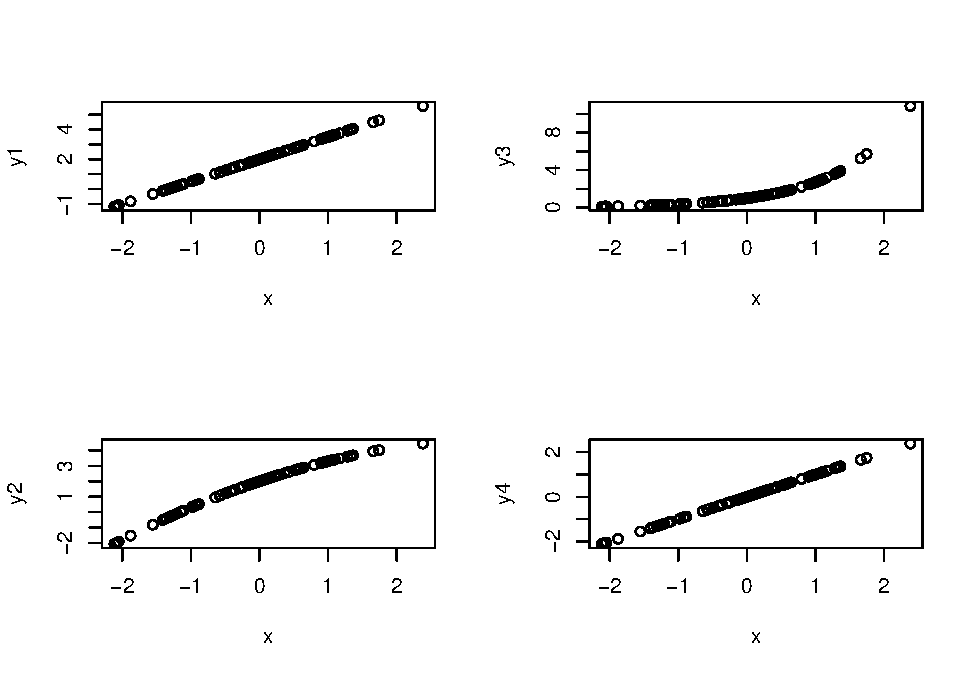
\includegraphics{_main_files/figure-latex/modelo lineal-1.pdf}

\begin{Shaded}
\begin{Highlighting}[]
\KeywordTok{layout}\NormalTok{(}\DecValTok{1}\NormalTok{)}
\end{Highlighting}
\end{Shaded}

\hypertarget{correlaciuxf3n-lineal-simple}{%
\section{Correlación lineal simple}\label{correlaciuxf3n-lineal-simple}}

\begin{Shaded}
\begin{Highlighting}[]
\NormalTok{x <-}\StringTok{ }\KeywordTok{rnorm}\NormalTok{(}\DecValTok{100}\NormalTok{)}
\NormalTok{e <-}\StringTok{ }\KeywordTok{rnorm}\NormalTok{(}\DecValTok{100}\NormalTok{, }\DataTypeTok{mean =} \DecValTok{0}\NormalTok{, }\DataTypeTok{sd =} \DecValTok{1}\NormalTok{)}
\NormalTok{y <-}\StringTok{ }\DecValTok{2} \OperatorTok{+}\StringTok{ }\FloatTok{1.5}\OperatorTok{*}\NormalTok{x }\OperatorTok{+}\StringTok{ }\NormalTok{e}
\KeywordTok{plot}\NormalTok{(x, y)}
\end{Highlighting}
\end{Shaded}

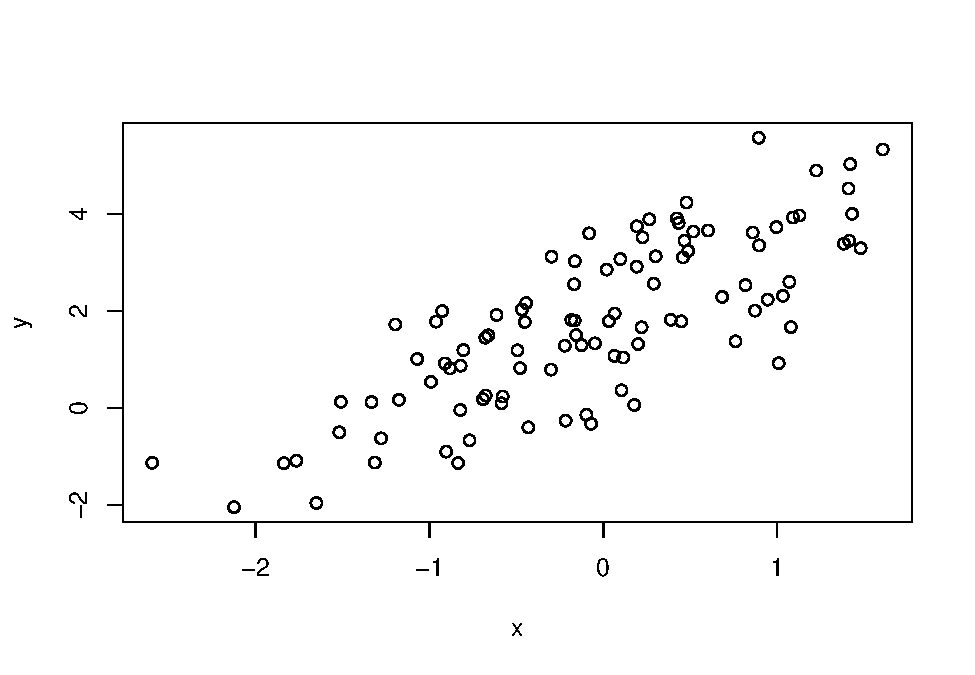
\includegraphics{_main_files/figure-latex/corr-1.pdf}

\begin{Shaded}
\begin{Highlighting}[]
\CommentTok{# Covarianza}
\KeywordTok{cov}\NormalTok{(x, y)}
\end{Highlighting}
\end{Shaded}

\begin{verbatim}
## [1] 1.21263
\end{verbatim}

\begin{Shaded}
\begin{Highlighting}[]
\CommentTok{# Correlación producto-momento de Pearson}
\KeywordTok{cov}\NormalTok{(x, y)}\OperatorTok{/}\NormalTok{(}\KeywordTok{sd}\NormalTok{(x)}\OperatorTok{*}\KeywordTok{sd}\NormalTok{(y))}
\end{Highlighting}
\end{Shaded}

\begin{verbatim}
## [1] 0.7897866
\end{verbatim}

\begin{Shaded}
\begin{Highlighting}[]
\KeywordTok{cor}\NormalTok{(x, y, }\DataTypeTok{method =} \StringTok{"pearson"}\NormalTok{)}
\end{Highlighting}
\end{Shaded}

\begin{verbatim}
## [1] 0.7897866
\end{verbatim}

\begin{Shaded}
\begin{Highlighting}[]
\KeywordTok{cor.test}\NormalTok{(x, y)}
\end{Highlighting}
\end{Shaded}

\begin{verbatim}
## 
##  Pearson's product-moment correlation
## 
## data:  x and y
## t = 12.747, df = 98, p-value < 2.2e-16
## alternative hypothesis: true correlation is not equal to 0
## 95 percent confidence interval:
##  0.7023179 0.8537620
## sample estimates:
##       cor 
## 0.7897866
\end{verbatim}

\begin{Shaded}
\begin{Highlighting}[]
\CommentTok{# Monotonía}
\KeywordTok{layout}\NormalTok{(}\KeywordTok{matrix}\NormalTok{(}\DecValTok{1}\OperatorTok{:}\DecValTok{4}\NormalTok{, }\DecValTok{2}\NormalTok{, }\DecValTok{2}\NormalTok{))}
\NormalTok{x1 <-}\StringTok{ }\KeywordTok{seq}\NormalTok{(}\DecValTok{1}\NormalTok{, }\DecValTok{10}\NormalTok{, }\DataTypeTok{length =} \DecValTok{100}\NormalTok{)}
\NormalTok{y1 <-}\StringTok{ }\FloatTok{0.5} \OperatorTok{+}\StringTok{ }\DecValTok{2}\OperatorTok{*}\NormalTok{x1}
\KeywordTok{plot}\NormalTok{(x1, y1, }\DataTypeTok{type =} \StringTok{"l"}\NormalTok{)}
\NormalTok{y2 <-}\StringTok{ }\FloatTok{0.5} \OperatorTok{+}\StringTok{ }\DecValTok{2}\OperatorTok{*}\NormalTok{x1 }\OperatorTok{-}\StringTok{ }\FloatTok{0.2}\OperatorTok{*}\NormalTok{x1}\OperatorTok{^}\DecValTok{2}
\KeywordTok{plot}\NormalTok{(x1, y2, }\DataTypeTok{type =} \StringTok{"l"}\NormalTok{)}
\NormalTok{y3 <-}\StringTok{ }\KeywordTok{exp}\NormalTok{(}\OperatorTok{-}\DecValTok{5} \OperatorTok{+}\StringTok{ }\NormalTok{x1)}
\KeywordTok{plot}\NormalTok{(x1, y3, }\DataTypeTok{type =} \StringTok{"l"}\NormalTok{)}
\NormalTok{y4 <-}\StringTok{ }\KeywordTok{exp}\NormalTok{(}\OperatorTok{-}\DecValTok{5} \OperatorTok{+}\StringTok{ }\NormalTok{x1)}\OperatorTok{/}\NormalTok{(}\DecValTok{1} \OperatorTok{+}\StringTok{ }\KeywordTok{exp}\NormalTok{(}\OperatorTok{-}\DecValTok{5} \OperatorTok{+}\StringTok{ }\NormalTok{x1))}
\KeywordTok{plot}\NormalTok{(x1, y4, }\DataTypeTok{type =} \StringTok{"l"}\NormalTok{)}
\end{Highlighting}
\end{Shaded}

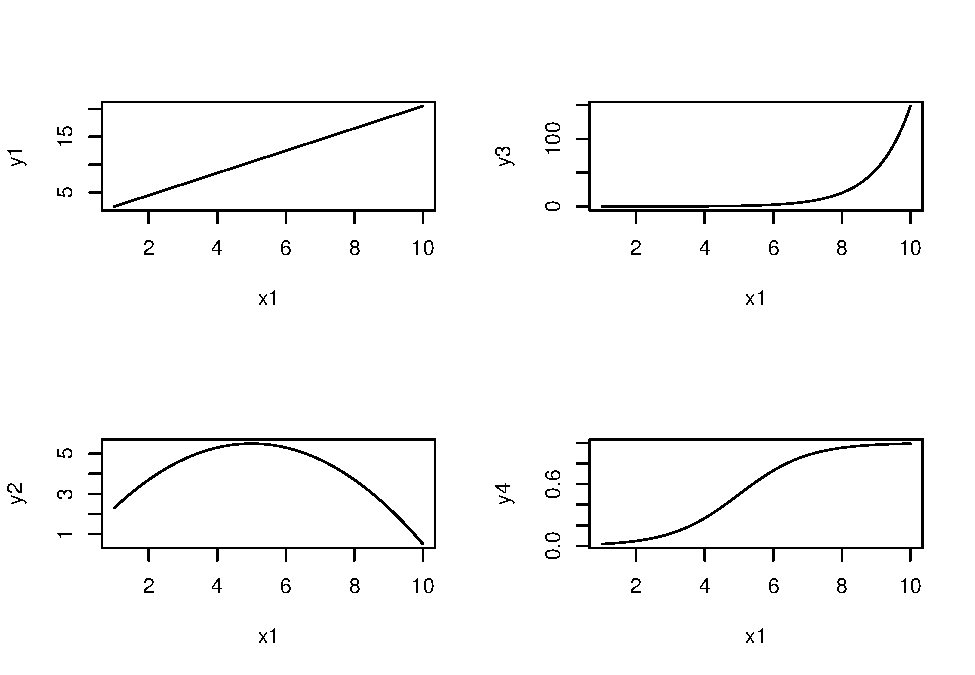
\includegraphics{_main_files/figure-latex/corr-2.pdf}

\begin{Shaded}
\begin{Highlighting}[]
\KeywordTok{layout}\NormalTok{(}\DecValTok{1}\NormalTok{)}

\CommentTok{# Correlación de Spearman}
\KeywordTok{cor}\NormalTok{(x1, y4, }\DataTypeTok{method =} \StringTok{"spearman"}\NormalTok{)}
\end{Highlighting}
\end{Shaded}

\begin{verbatim}
## [1] 1
\end{verbatim}

\begin{Shaded}
\begin{Highlighting}[]
\NormalTok{xrango <-}\StringTok{ }\KeywordTok{rank}\NormalTok{(x1) }
\NormalTok{yrango <-}\StringTok{ }\KeywordTok{rank}\NormalTok{(y4)}
\KeywordTok{plot}\NormalTok{(xrango, yrango)}
\end{Highlighting}
\end{Shaded}

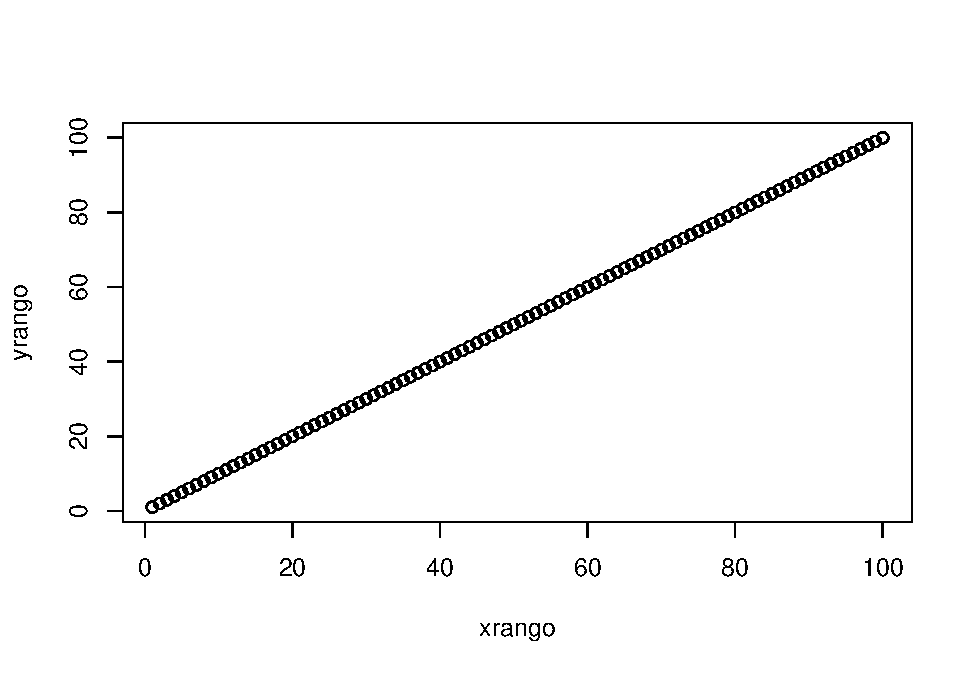
\includegraphics{_main_files/figure-latex/corr-3.pdf}

\begin{Shaded}
\begin{Highlighting}[]
\KeywordTok{cor}\NormalTok{(xrango, yrango, }\DataTypeTok{method =} \StringTok{"spearman"}\NormalTok{)}
\end{Highlighting}
\end{Shaded}

\begin{verbatim}
## [1] 1
\end{verbatim}

\hypertarget{matrices-de-correlaciuxf3n}{%
\section{Matrices de correlación}\label{matrices-de-correlaciuxf3n}}

A continuación se presentan las medidas del tamaño corporal en adultos de tres especies de pinguinos en islas del Archipiélago Palmer, Antártida.

\begin{Shaded}
\begin{Highlighting}[]
\KeywordTok{library}\NormalTok{(palmerpenguins)}
\end{Highlighting}
\end{Shaded}

\begin{verbatim}
## Warning: package 'palmerpenguins' was built under R version 4.0.5
\end{verbatim}

\begin{Shaded}
\begin{Highlighting}[]
\KeywordTok{str}\NormalTok{(penguins)}
\end{Highlighting}
\end{Shaded}

\begin{verbatim}
## tibble [344 x 8] (S3: tbl_df/tbl/data.frame)
##  $ species          : Factor w/ 3 levels "Adelie","Chinstrap",..: 1 1 1 1 1 1 1 1 1 1 ...
##  $ island           : Factor w/ 3 levels "Biscoe","Dream",..: 3 3 3 3 3 3 3 3 3 3 ...
##  $ bill_length_mm   : num [1:344] 39.1 39.5 40.3 NA 36.7 39.3 38.9 39.2 34.1 42 ...
##  $ bill_depth_mm    : num [1:344] 18.7 17.4 18 NA 19.3 20.6 17.8 19.6 18.1 20.2 ...
##  $ flipper_length_mm: int [1:344] 181 186 195 NA 193 190 181 195 193 190 ...
##  $ body_mass_g      : int [1:344] 3750 3800 3250 NA 3450 3650 3625 4675 3475 4250 ...
##  $ sex              : Factor w/ 2 levels "female","male": 2 1 1 NA 1 2 1 2 NA NA ...
##  $ year             : int [1:344] 2007 2007 2007 2007 2007 2007 2007 2007 2007 2007 ...
\end{verbatim}

\begin{Shaded}
\begin{Highlighting}[]
\KeywordTok{cor}\NormalTok{(penguins[, }\DecValTok{3}\OperatorTok{:}\DecValTok{6}\NormalTok{], }\DataTypeTok{use =} \StringTok{"complete.obs"}\NormalTok{)}
\end{Highlighting}
\end{Shaded}

\begin{verbatim}
##                   bill_length_mm bill_depth_mm flipper_length_mm body_mass_g
## bill_length_mm         1.0000000    -0.2350529         0.6561813   0.5951098
## bill_depth_mm         -0.2350529     1.0000000        -0.5838512  -0.4719156
## flipper_length_mm      0.6561813    -0.5838512         1.0000000   0.8712018
## body_mass_g            0.5951098    -0.4719156         0.8712018   1.0000000
\end{verbatim}

\begin{Shaded}
\begin{Highlighting}[]
\KeywordTok{pairs}\NormalTok{(penguins[, }\DecValTok{3}\OperatorTok{:}\DecValTok{6}\NormalTok{])}
\end{Highlighting}
\end{Shaded}

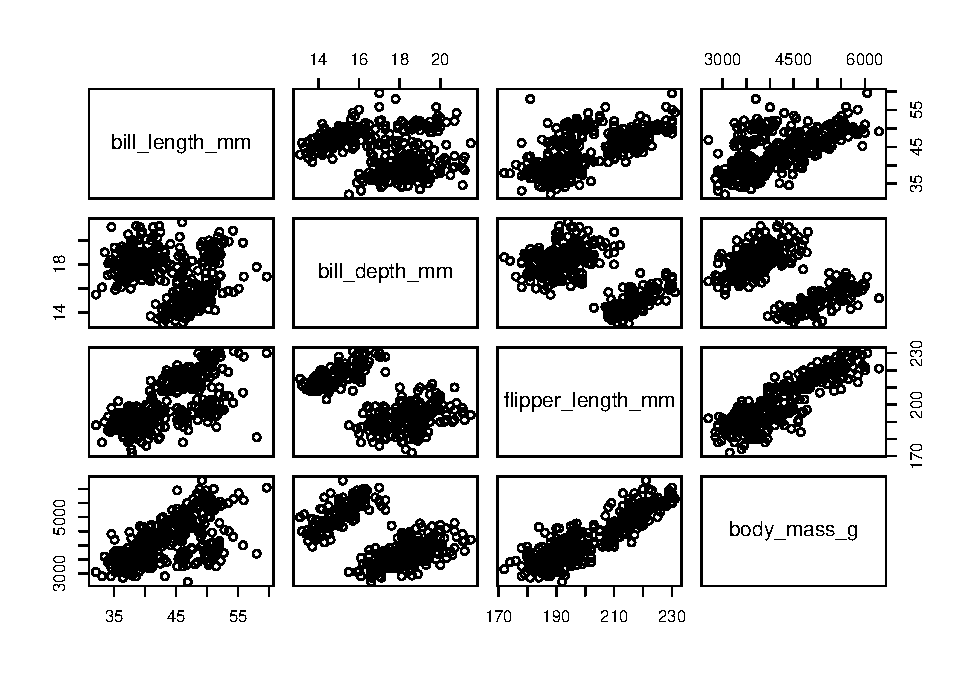
\includegraphics{_main_files/figure-latex/mat corr-1.pdf}

\begin{Shaded}
\begin{Highlighting}[]
\NormalTok{Ad <-}\StringTok{ }\KeywordTok{subset}\NormalTok{(penguins, species }\OperatorTok{==}\StringTok{ "Adelie"}\NormalTok{)}
\KeywordTok{round}\NormalTok{(}\KeywordTok{cor}\NormalTok{(Ad[, }\DecValTok{3}\OperatorTok{:}\DecValTok{6}\NormalTok{], }\DataTypeTok{use =} \StringTok{"complete.obs"}\NormalTok{), }\DecValTok{2}\NormalTok{)}
\end{Highlighting}
\end{Shaded}

\begin{verbatim}
##                   bill_length_mm bill_depth_mm flipper_length_mm body_mass_g
## bill_length_mm              1.00          0.39              0.33        0.55
## bill_depth_mm               0.39          1.00              0.31        0.58
## flipper_length_mm           0.33          0.31              1.00        0.47
## body_mass_g                 0.55          0.58              0.47        1.00
\end{verbatim}

\begin{Shaded}
\begin{Highlighting}[]
\KeywordTok{library}\NormalTok{(Hmisc)}
\end{Highlighting}
\end{Shaded}

\begin{verbatim}
## Loading required package: lattice
\end{verbatim}

\begin{verbatim}
## Loading required package: survival
\end{verbatim}

\begin{verbatim}
## Loading required package: Formula
\end{verbatim}

\begin{verbatim}
## Loading required package: ggplot2
\end{verbatim}

\begin{verbatim}
## Warning: package 'ggplot2' was built under R version 4.0.5
\end{verbatim}

\begin{verbatim}
## 
## Attaching package: 'Hmisc'
\end{verbatim}

\begin{verbatim}
## The following objects are masked from 'package:base':
## 
##     format.pval, units
\end{verbatim}

\begin{Shaded}
\begin{Highlighting}[]
\NormalTok{matriz.corr <-}\StringTok{ }\KeywordTok{rcorr}\NormalTok{(}\KeywordTok{as.matrix}\NormalTok{(Ad[, }\DecValTok{3}\OperatorTok{:}\DecValTok{6}\NormalTok{]), }\DataTypeTok{type =} \StringTok{"pearson"}\NormalTok{)}
\NormalTok{matriz.corr}
\end{Highlighting}
\end{Shaded}

\begin{verbatim}
##                   bill_length_mm bill_depth_mm flipper_length_mm body_mass_g
## bill_length_mm              1.00          0.39              0.33        0.55
## bill_depth_mm               0.39          1.00              0.31        0.58
## flipper_length_mm           0.33          0.31              1.00        0.47
## body_mass_g                 0.55          0.58              0.47        1.00
## 
## n= 151 
## 
## 
## P
##                   bill_length_mm bill_depth_mm flipper_length_mm body_mass_g
## bill_length_mm                   0e+00         0e+00             0e+00      
## bill_depth_mm     0e+00                        1e-04             0e+00      
## flipper_length_mm 0e+00          1e-04                           0e+00      
## body_mass_g       0e+00          0e+00         0e+00
\end{verbatim}

\begin{Shaded}
\begin{Highlighting}[]
\KeywordTok{p.adjust}\NormalTok{(matriz.corr}\OperatorTok{$}\NormalTok{P, }\DataTypeTok{method =} \StringTok{"holm"}\NormalTok{) }
\end{Highlighting}
\end{Shaded}

\begin{verbatim}
##  [1]           NA 4.004485e-06 1.786194e-04 2.953193e-12 4.004485e-06           NA
##  [7] 2.437897e-04 1.199041e-13 1.786194e-04 2.437897e-04           NA 1.074612e-08
## [13] 2.953193e-12 1.199041e-13 1.074612e-08           NA
\end{verbatim}

\hypertarget{regresiuxf3n-lineal-simple}{%
\section{Regresión lineal simple}\label{regresiuxf3n-lineal-simple}}

\[y = \beta_0 + \beta_1 x + \epsilon\]
\[\epsilon \sim N(0, \sigma^2)\]

\begin{Shaded}
\begin{Highlighting}[]
\NormalTok{x <-}\StringTok{ }\KeywordTok{rnorm}\NormalTok{(}\DecValTok{100}\NormalTok{)}
\NormalTok{e <-}\StringTok{ }\KeywordTok{rnorm}\NormalTok{(}\DecValTok{100}\NormalTok{, }\DataTypeTok{mean =} \DecValTok{0}\NormalTok{, }\DataTypeTok{sd =} \DecValTok{1}\NormalTok{)}
\NormalTok{y <-}\StringTok{ }\DecValTok{2} \OperatorTok{+}\StringTok{ }\FloatTok{1.5}\OperatorTok{*}\NormalTok{x }\OperatorTok{+}\StringTok{ }\NormalTok{e}
\KeywordTok{plot}\NormalTok{(x, y)}

\NormalTok{datos <-}\StringTok{ }\KeywordTok{data.frame}\NormalTok{(x, y)}
\NormalTok{reg.simple <-}\StringTok{ }\KeywordTok{lm}\NormalTok{(y }\OperatorTok{~}\StringTok{ }\NormalTok{x, }\DataTypeTok{data =}\NormalTok{ datos)}
\KeywordTok{summary}\NormalTok{(reg.simple)}
\end{Highlighting}
\end{Shaded}

\begin{verbatim}
## 
## Call:
## lm(formula = y ~ x, data = datos)
## 
## Residuals:
##      Min       1Q   Median       3Q      Max 
## -2.51881 -0.65262 -0.06149  0.59194  3.05669 
## 
## Coefficients:
##             Estimate Std. Error t value Pr(>|t|)    
## (Intercept)   1.9948     0.0996   20.03   <2e-16 ***
## x             1.4928     0.1020   14.64   <2e-16 ***
## ---
## Signif. codes:  0 '***' 0.001 '**' 0.01 '*' 0.05 '.' 0.1 ' ' 1
## 
## Residual standard error: 0.996 on 98 degrees of freedom
## Multiple R-squared:  0.6863, Adjusted R-squared:  0.6831 
## F-statistic: 214.4 on 1 and 98 DF,  p-value: < 2.2e-16
\end{verbatim}

\begin{Shaded}
\begin{Highlighting}[]
\CommentTok{# Pendiente}
\KeywordTok{cov}\NormalTok{(x, y)}\OperatorTok{/}\KeywordTok{var}\NormalTok{(x) }
\end{Highlighting}
\end{Shaded}

\begin{verbatim}
## [1] 1.492825
\end{verbatim}

\begin{Shaded}
\begin{Highlighting}[]
\KeywordTok{summary}\NormalTok{(reg.simple)}\OperatorTok{$}\NormalTok{coeff}
\end{Highlighting}
\end{Shaded}

\begin{verbatim}
##             Estimate Std. Error  t value     Pr(>|t|)
## (Intercept) 1.994796 0.09960184 20.02770 2.042392e-36
## x           1.492825 0.10195980 14.64131 2.072208e-26
\end{verbatim}

\begin{Shaded}
\begin{Highlighting}[]
\CommentTok{# Coeficiente de determinación}
\NormalTok{SCE <-}\StringTok{ }\KeywordTok{sum}\NormalTok{((}\KeywordTok{mean}\NormalTok{(datos}\OperatorTok{$}\NormalTok{y) }\OperatorTok{-}\StringTok{ }\NormalTok{reg.simple}\OperatorTok{$}\NormalTok{fitted)}\OperatorTok{^}\DecValTok{2}\NormalTok{) }\CommentTok{# suma de cuadrados explicada}
\NormalTok{SCT <-}\StringTok{ }\KeywordTok{sum}\NormalTok{((datos}\OperatorTok{$}\NormalTok{y }\OperatorTok{-}\StringTok{ }\KeywordTok{mean}\NormalTok{(datos}\OperatorTok{$}\NormalTok{y))}\OperatorTok{^}\DecValTok{2}\NormalTok{) }\CommentTok{# suma de cuadrados total}
\NormalTok{R2 <-}\StringTok{ }\NormalTok{SCE}\OperatorTok{/}\NormalTok{SCT}
\NormalTok{R2}
\end{Highlighting}
\end{Shaded}

\begin{verbatim}
## [1] 0.6862674
\end{verbatim}

\begin{Shaded}
\begin{Highlighting}[]
\KeywordTok{summary}\NormalTok{(reg.simple)}\OperatorTok{$}\NormalTok{r.squared }
\end{Highlighting}
\end{Shaded}

\begin{verbatim}
## [1] 0.6862674
\end{verbatim}

\begin{Shaded}
\begin{Highlighting}[]
\CommentTok{# Gráfico}
\KeywordTok{plot}\NormalTok{(x, y)}
\KeywordTok{abline}\NormalTok{(reg.simple, }\DataTypeTok{lwd =} \DecValTok{2}\NormalTok{)}
\end{Highlighting}
\end{Shaded}

\includegraphics{_main_files/figure-latex/regresión simple-1.pdf}

\hypertarget{relaciuxf3n-entre-regresiuxf3n-y-correlaciuxf3n}{%
\section{Relación entre regresión y correlación}\label{relaciuxf3n-entre-regresiuxf3n-y-correlaciuxf3n}}

\begin{Shaded}
\begin{Highlighting}[]
\NormalTok{beta <-}\StringTok{ }\KeywordTok{summary}\NormalTok{(reg.simple)}\OperatorTok{$}\NormalTok{coeff[}\DecValTok{2}\NormalTok{, }\DecValTok{1}\NormalTok{]}
\NormalTok{beta}\OperatorTok{*}\KeywordTok{sd}\NormalTok{(x)}\OperatorTok{/}\KeywordTok{sd}\NormalTok{(y)}
\end{Highlighting}
\end{Shaded}

\begin{verbatim}
## [1] 0.8284126
\end{verbatim}

\begin{Shaded}
\begin{Highlighting}[]
\KeywordTok{sqrt}\NormalTok{(}\KeywordTok{summary}\NormalTok{(reg.simple)}\OperatorTok{$}\NormalTok{r.squared)}
\end{Highlighting}
\end{Shaded}

\begin{verbatim}
## [1] 0.8284126
\end{verbatim}

\begin{Shaded}
\begin{Highlighting}[]
\KeywordTok{cor}\NormalTok{(x, y)}
\end{Highlighting}
\end{Shaded}

\begin{verbatim}
## [1] 0.8284126
\end{verbatim}

\hypertarget{matrices-de-gruxe1ficos-de-dispersiuxf3n}{%
\section{Matrices de gráficos de dispersión}\label{matrices-de-gruxe1ficos-de-dispersiuxf3n}}

\begin{Shaded}
\begin{Highlighting}[]
\KeywordTok{pairs}\NormalTok{(Ad[, }\DecValTok{3}\OperatorTok{:}\DecValTok{6}\NormalTok{], }\DataTypeTok{pch =} \DecValTok{19}\NormalTok{, }\DataTypeTok{col =} \StringTok{"blue"}\NormalTok{, }\DataTypeTok{lower.panel =} \OtherTok{NULL}\NormalTok{)}
\end{Highlighting}
\end{Shaded}

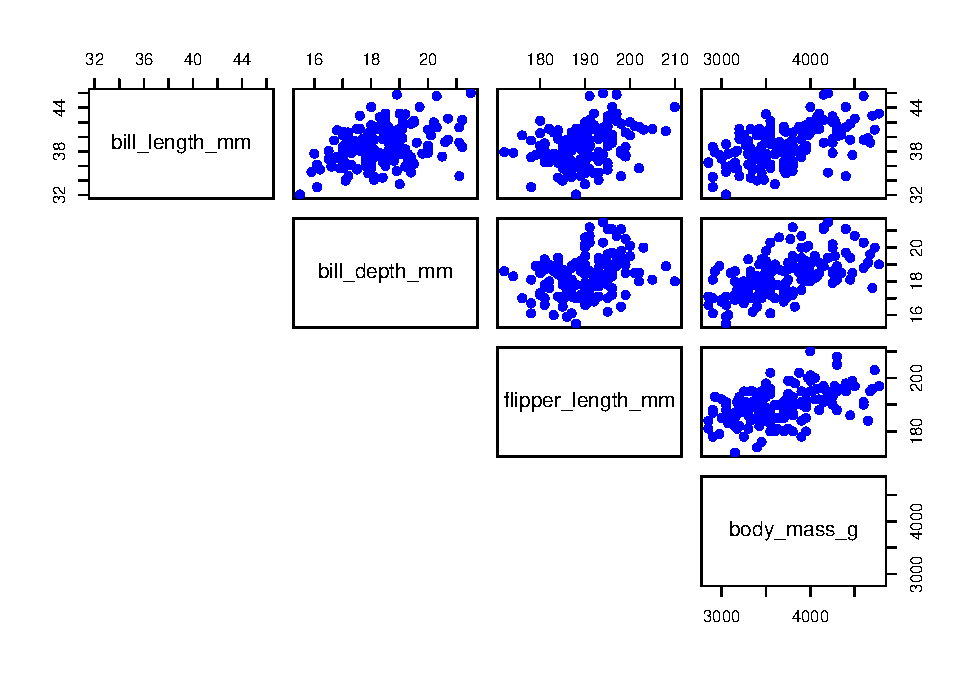
\includegraphics{_main_files/figure-latex/scatterplot matrix-1.pdf}

\begin{Shaded}
\begin{Highlighting}[]
\KeywordTok{pairs}\NormalTok{(penguins[, }\DecValTok{3}\OperatorTok{:}\DecValTok{6}\NormalTok{], }\DataTypeTok{pch =} \DecValTok{19}\NormalTok{, }\DataTypeTok{col =} \KeywordTok{c}\NormalTok{(}\StringTok{"red"}\NormalTok{, }\StringTok{"orange"}\NormalTok{, }\StringTok{"blue"}\NormalTok{)[penguins}\OperatorTok{$}\NormalTok{species], }\DataTypeTok{lower.panel =} \OtherTok{NULL}\NormalTok{)}
\end{Highlighting}
\end{Shaded}

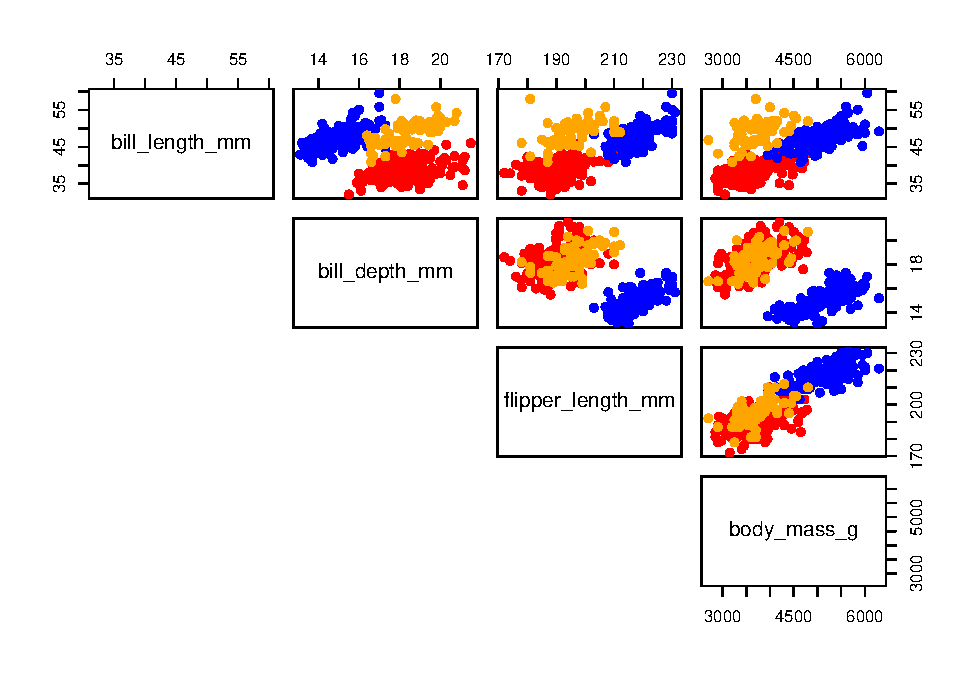
\includegraphics{_main_files/figure-latex/scatterplot matrix-2.pdf}

\begin{Shaded}
\begin{Highlighting}[]
\KeywordTok{library}\NormalTok{(psych)}
\end{Highlighting}
\end{Shaded}

\begin{verbatim}
## 
## Attaching package: 'psych'
\end{verbatim}

\begin{verbatim}
## The following object is masked from 'package:Hmisc':
## 
##     describe
\end{verbatim}

\begin{verbatim}
## The following objects are masked from 'package:ggplot2':
## 
##     %+%, alpha
\end{verbatim}

\begin{Shaded}
\begin{Highlighting}[]
\KeywordTok{pairs.panels}\NormalTok{(Ad[, }\DecValTok{3}\OperatorTok{:}\DecValTok{6}\NormalTok{], }
             \DataTypeTok{method =} \StringTok{"pearson"}\NormalTok{, }\CommentTok{# correlación}
             \DataTypeTok{density =} \OtherTok{FALSE}\NormalTok{,  }\CommentTok{# gráficos de densidad}
             \DataTypeTok{ellipses =} \OtherTok{FALSE}\NormalTok{, }\CommentTok{# elipses de confianza}
             \DataTypeTok{lm =} \OtherTok{TRUE}\NormalTok{) }\CommentTok{# recta}
\end{Highlighting}
\end{Shaded}

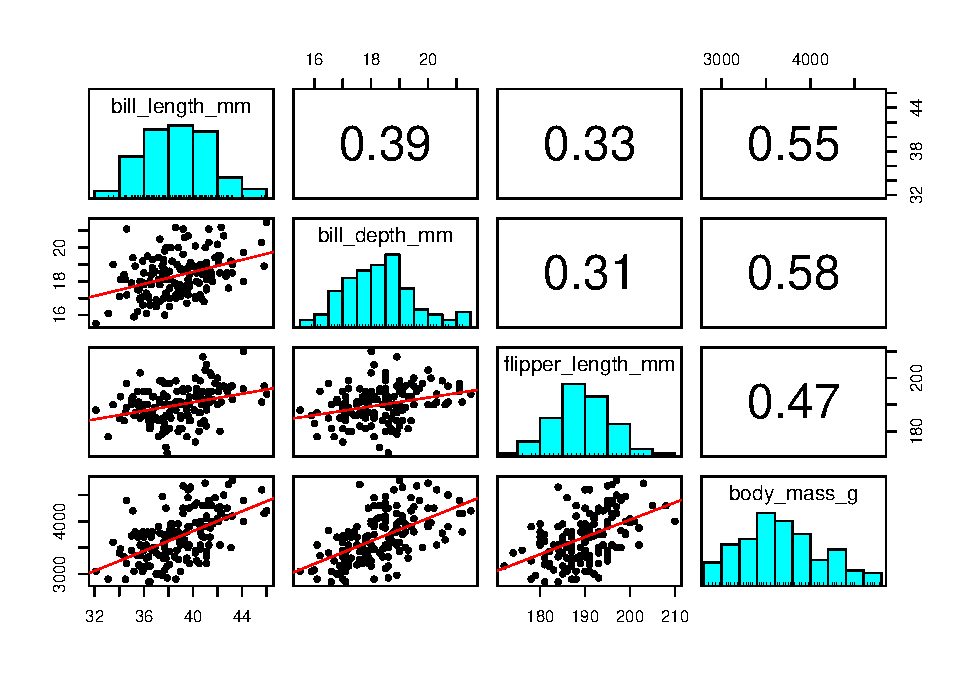
\includegraphics{_main_files/figure-latex/scatterplot matrix-3.pdf}

\hypertarget{regresiuxf3n-lineal-multiple}{%
\section{Regresión lineal multiple}\label{regresiuxf3n-lineal-multiple}}

\[y = \beta_0 + \beta_1 x_1 + \beta_2 x_2 + ... + \beta_n x_n + \epsilon\]
\[\epsilon \sim N(0, \sigma^2)\]

Analizaremos la relación entre la longitud del pico (´bill\_length\_mm´), masa corporal (\texttt{body\_mass\_g}) y alto del pico (\texttt{bill\_depth\_mm}) en pinguinos Adelia (\(Pygoscelis adeliae\)).

\begin{Shaded}
\begin{Highlighting}[]
\NormalTok{model.Ad <-}\StringTok{ }\KeywordTok{lm}\NormalTok{(bill_length_mm }\OperatorTok{~}\StringTok{ }\NormalTok{body_mass_g }\OperatorTok{+}\StringTok{ }\NormalTok{bill_depth_mm, }\DataTypeTok{data =}\NormalTok{ Ad)}
\KeywordTok{summary}\NormalTok{(model.Ad)}
\end{Highlighting}
\end{Shaded}

\begin{verbatim}
## 
## Call:
## lm(formula = bill_length_mm ~ body_mass_g + bill_depth_mm, data = Ad)
## 
## Residuals:
##     Min      1Q  Median      3Q     Max 
## -6.8363 -1.5105  0.0952  1.4967  5.6090 
## 
## Coefficients:
##                Estimate Std. Error t value Pr(>|t|)    
## (Intercept)   2.386e+01  2.752e+00   8.671 7.00e-15 ***
## body_mass_g   2.811e-03  4.853e-04   5.792 4.02e-08 ***
## bill_depth_mm 2.466e-01  1.829e-01   1.348     0.18    
## ---
## Signif. codes:  0 '***' 0.001 '**' 0.01 '*' 0.05 '.' 0.1 ' ' 1
## 
## Residual standard error: 2.228 on 148 degrees of freedom
##   (1 observation deleted due to missingness)
## Multiple R-squared:  0.3097, Adjusted R-squared:  0.3004 
## F-statistic: 33.21 on 2 and 148 DF,  p-value: 1.222e-12
\end{verbatim}

\begin{Shaded}
\begin{Highlighting}[]
\NormalTok{sum.cuad.exp <-}\StringTok{ }\KeywordTok{sum}\NormalTok{((}\KeywordTok{mean}\NormalTok{(}\KeywordTok{na.omit}\NormalTok{(Ad}\OperatorTok{$}\NormalTok{bill_length_mm)) }\OperatorTok{-}\StringTok{ }\NormalTok{model.Ad}\OperatorTok{$}\NormalTok{fitted)}\OperatorTok{^}\DecValTok{2}\NormalTok{)}
\NormalTok{sum.cuad.tot <-}\StringTok{ }\KeywordTok{sum}\NormalTok{((}\KeywordTok{na.omit}\NormalTok{(Ad}\OperatorTok{$}\NormalTok{bill_length_mm) }\OperatorTok{-}\StringTok{ }\KeywordTok{mean}\NormalTok{(}\KeywordTok{na.omit}\NormalTok{(Ad}\OperatorTok{$}\NormalTok{bill_length_mm)))}\OperatorTok{^}\DecValTok{2}\NormalTok{)}
\NormalTok{R2 <-}\StringTok{ }\NormalTok{sum.cuad.exp}\OperatorTok{/}\NormalTok{sum.cuad.tot}
\NormalTok{R2}
\end{Highlighting}
\end{Shaded}

\begin{verbatim}
## [1] 0.3097341
\end{verbatim}

\begin{Shaded}
\begin{Highlighting}[]
\CommentTok{# Gráfico de dispersión con plano de regresión}
\KeywordTok{library}\NormalTok{(plot3D)}
\NormalTok{x <-}\StringTok{ }\NormalTok{Ad}\OperatorTok{$}\NormalTok{body_mass_g}
\NormalTok{y <-}\StringTok{ }\NormalTok{Ad}\OperatorTok{$}\NormalTok{bill_depth_mm}
\NormalTok{z <-}\StringTok{ }\NormalTok{Ad}\OperatorTok{$}\NormalTok{bill_length_mm}
\NormalTok{x.pred <-}\StringTok{ }\KeywordTok{seq}\NormalTok{(}\KeywordTok{min}\NormalTok{(x, }\DataTypeTok{na.rm =}\NormalTok{ T), }\KeywordTok{max}\NormalTok{(x, }\DataTypeTok{na.rm =}\NormalTok{ T), }\DataTypeTok{length =} \DecValTok{30}\NormalTok{)}
\NormalTok{y.pred <-}\StringTok{ }\KeywordTok{seq}\NormalTok{(}\KeywordTok{min}\NormalTok{(y, }\DataTypeTok{na.rm =}\NormalTok{ T), }\KeywordTok{max}\NormalTok{(y, }\DataTypeTok{na.rm =}\NormalTok{ T), }\DataTypeTok{length =} \DecValTok{30}\NormalTok{)}
\NormalTok{xy <-}\StringTok{ }\KeywordTok{expand.grid}\NormalTok{(}\DataTypeTok{body_mass_g =}\NormalTok{ x.pred, }\DataTypeTok{bill_depth_mm =}\NormalTok{ y.pred)}
\NormalTok{z.pred <-}\StringTok{ }\KeywordTok{matrix}\NormalTok{(}\KeywordTok{predict}\NormalTok{(model.Ad, }\DataTypeTok{newdata =}\NormalTok{ xy), }\DataTypeTok{nrow =} \DecValTok{30}\NormalTok{, }\DataTypeTok{ncol =} \DecValTok{30}\NormalTok{)}
\KeywordTok{scatter3D}\NormalTok{(x, y, z, }\DataTypeTok{pch =} \DecValTok{18}\NormalTok{, }\DataTypeTok{cex =} \DecValTok{2}\NormalTok{, }
          \DataTypeTok{theta =} \DecValTok{35}\NormalTok{, }\DataTypeTok{phi =} \DecValTok{20}\NormalTok{, }\DataTypeTok{ticktype =} \StringTok{"detailed"}\NormalTok{,}
          \DataTypeTok{xlab =} \StringTok{"Masa corporal"}\NormalTok{, }\DataTypeTok{ylab =} \StringTok{"Alto del pico"}\NormalTok{, }
          \DataTypeTok{zlab =} \StringTok{"Longitud del pico"}\NormalTok{,  }
          \DataTypeTok{surf =} \KeywordTok{list}\NormalTok{(}\DataTypeTok{x =}\NormalTok{ x.pred, }\DataTypeTok{y =}\NormalTok{ y.pred, }\DataTypeTok{z =}\NormalTok{ z.pred, }\DataTypeTok{facets =} \OtherTok{NA}\NormalTok{))}
\end{Highlighting}
\end{Shaded}

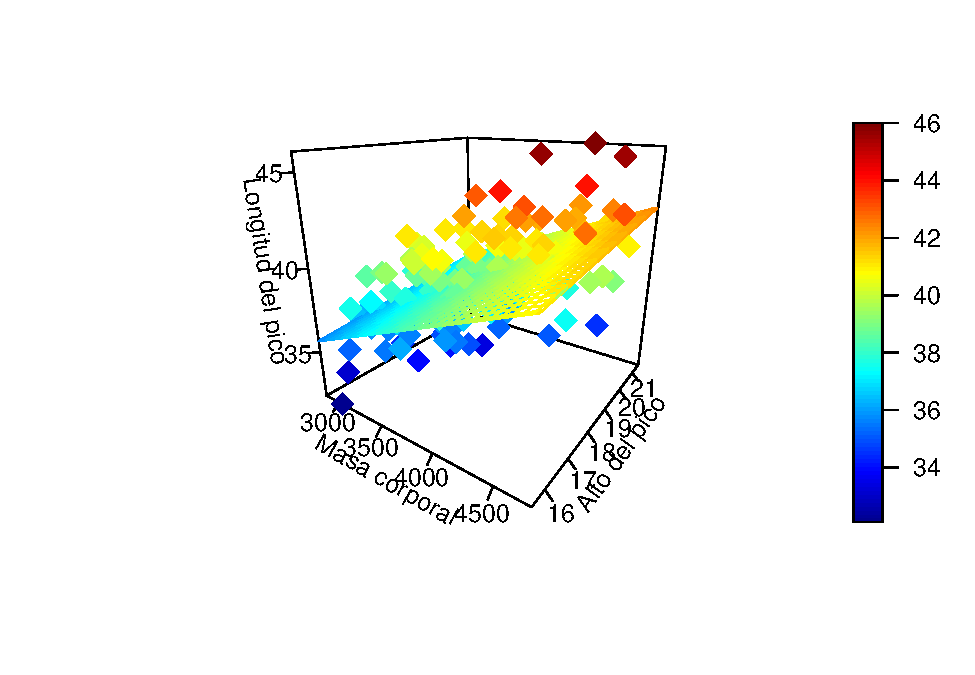
\includegraphics{_main_files/figure-latex/regresion multiple-1.pdf}

\begin{Shaded}
\begin{Highlighting}[]
\KeywordTok{library}\NormalTok{(visreg)}
\NormalTok{Ad}\OperatorTok{$}\NormalTok{bill_depth_cat <-}\StringTok{ }\KeywordTok{cut}\NormalTok{(Ad}\OperatorTok{$}\NormalTok{bill_depth_mm, }\DecValTok{3}\NormalTok{, }
                         \DataTypeTok{labels =} \KeywordTok{c}\NormalTok{(}\StringTok{"Pequeño"}\NormalTok{, }\StringTok{"Mediano"}\NormalTok{, }\StringTok{"Grande"}\NormalTok{))}
\NormalTok{model.Ad_cat <-}\StringTok{ }\KeywordTok{lm}\NormalTok{(bill_length_mm }\OperatorTok{~}\StringTok{ }\NormalTok{body_mass_g }\OperatorTok{+}\StringTok{ }\NormalTok{bill_depth_cat, }\DataTypeTok{data =}\NormalTok{ Ad)}
\KeywordTok{visreg}\NormalTok{(model.Ad_cat, }\StringTok{"body_mass_g"}\NormalTok{, }\StringTok{"bill_depth_cat"}\NormalTok{, }\DataTypeTok{gg =} \OtherTok{TRUE}\NormalTok{)}
\end{Highlighting}
\end{Shaded}

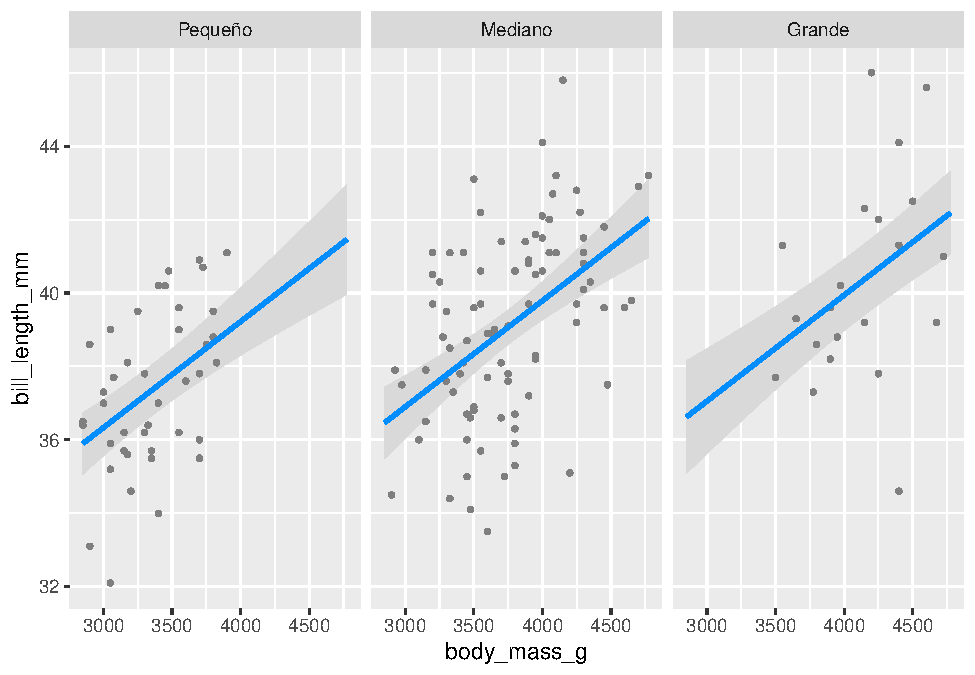
\includegraphics{_main_files/figure-latex/regresion multiple-2.pdf}

\hypertarget{variables-categuxf3ricas-dummies}{%
\section{\texorpdfstring{Variables categóricas (= \emph{dummies})}{Variables categóricas (= dummies)}}\label{variables-categuxf3ricas-dummies}}

\begin{Shaded}
\begin{Highlighting}[]
\NormalTok{model.penguins1 <-}\StringTok{ }\KeywordTok{lm}\NormalTok{(bill_length_mm }\OperatorTok{~}\StringTok{ }\NormalTok{body_mass_g }\OperatorTok{+}\StringTok{ }\NormalTok{species, }\DataTypeTok{data =}\NormalTok{ penguins)}
\KeywordTok{summary}\NormalTok{(model.penguins1)}
\end{Highlighting}
\end{Shaded}

\begin{verbatim}
## 
## Call:
## lm(formula = bill_length_mm ~ body_mass_g + species, data = penguins)
## 
## Residuals:
##     Min      1Q  Median      3Q     Max 
## -6.8129 -1.6718  0.1336  1.4720  9.2902 
## 
## Coefficients:
##                   Estimate Std. Error t value Pr(>|t|)    
## (Intercept)      2.492e+01  1.063e+00  23.443  < 2e-16 ***
## body_mass_g      3.749e-03  2.823e-04  13.276  < 2e-16 ***
## speciesChinstrap 9.921e+00  3.511e-01  28.258  < 2e-16 ***
## speciesGentoo    3.558e+00  4.858e-01   7.324 1.78e-12 ***
## ---
## Signif. codes:  0 '***' 0.001 '**' 0.01 '*' 0.05 '.' 0.1 ' ' 1
## 
## Residual standard error: 2.403 on 338 degrees of freedom
##   (2 observations deleted due to missingness)
## Multiple R-squared:  0.808,  Adjusted R-squared:  0.8063 
## F-statistic:   474 on 3 and 338 DF,  p-value: < 2.2e-16
\end{verbatim}

\begin{Shaded}
\begin{Highlighting}[]
\NormalTok{model.penguins2 <-}\StringTok{ }\KeywordTok{lm}\NormalTok{(bill_length_mm }\OperatorTok{~}\StringTok{ }\NormalTok{body_mass_g }\OperatorTok{+}\StringTok{ }\NormalTok{species }\OperatorTok{+}\StringTok{ }\NormalTok{body_mass_g}\OperatorTok{:}\NormalTok{species, }\DataTypeTok{data =}\NormalTok{ penguins)}
\KeywordTok{summary}\NormalTok{(model.penguins2)}
\end{Highlighting}
\end{Shaded}

\begin{verbatim}
## 
## Call:
## lm(formula = bill_length_mm ~ body_mass_g + species + body_mass_g:species, 
##     data = penguins)
## 
## Residuals:
##     Min      1Q  Median      3Q     Max 
## -6.4208 -1.6461  0.0919  1.4718  9.3138 
## 
## Coefficients:
##                                Estimate Std. Error t value Pr(>|t|)    
## (Intercept)                  26.9941391  1.5926015  16.950  < 2e-16 ***
## body_mass_g                   0.0031879  0.0004271   7.464 7.27e-13 ***
## speciesChinstrap              5.1800537  3.2746719   1.582    0.115    
## speciesGentoo                -0.2545907  2.7138655  -0.094    0.925    
## body_mass_g:speciesChinstrap  0.0012748  0.0008740   1.459    0.146    
## body_mass_g:speciesGentoo     0.0009030  0.0006066   1.489    0.138    
## ---
## Signif. codes:  0 '***' 0.001 '**' 0.01 '*' 0.05 '.' 0.1 ' ' 1
## 
## Residual standard error: 2.399 on 336 degrees of freedom
##   (2 observations deleted due to missingness)
## Multiple R-squared:  0.8098, Adjusted R-squared:  0.807 
## F-statistic: 286.1 on 5 and 336 DF,  p-value: < 2.2e-16
\end{verbatim}

\begin{Shaded}
\begin{Highlighting}[]
\KeywordTok{anova}\NormalTok{(model.penguins2)}
\end{Highlighting}
\end{Shaded}

\begin{verbatim}
## Analysis of Variance Table
## 
## Response: bill_length_mm
##                      Df Sum Sq Mean Sq  F value Pr(>F)    
## body_mass_g           1 3599.7  3599.7 625.5924 <2e-16 ***
## species               2 4612.5  2306.3 400.8045 <2e-16 ***
## body_mass_g:species   2   18.6     9.3   1.6159 0.2003    
## Residuals           336 1933.4     5.8                    
## ---
## Signif. codes:  0 '***' 0.001 '**' 0.01 '*' 0.05 '.' 0.1 ' ' 1
\end{verbatim}

\hypertarget{test-de-t}{%
\section{\texorpdfstring{Test de \emph{t}}{Test de t}}\label{test-de-t}}

Se muestran los tiempos de coagulación sanguínea (min) en conejos bajo el efecto de dos drogas (A y B).

\begin{Shaded}
\begin{Highlighting}[]
\NormalTok{t_coag <-}\StringTok{ }\KeywordTok{c}\NormalTok{(}\FloatTok{8.8}\NormalTok{, }\FloatTok{8.4}\NormalTok{, }\FloatTok{7.9}\NormalTok{, }\FloatTok{8.7}\NormalTok{, }\FloatTok{9.1}\NormalTok{, }\FloatTok{9.6}\NormalTok{, }\FloatTok{9.5}\NormalTok{, }
            \FloatTok{9.9}\NormalTok{, }\FloatTok{9.0}\NormalTok{, }\FloatTok{11.1}\NormalTok{, }\FloatTok{9.6}\NormalTok{, }\FloatTok{8.7}\NormalTok{, }\FloatTok{10.4}\NormalTok{, }\FloatTok{9.5}\NormalTok{) }
\NormalTok{droga <-}\StringTok{ }\KeywordTok{c}\NormalTok{(}\KeywordTok{rep}\NormalTok{(}\StringTok{"A"}\NormalTok{, }\DecValTok{7}\NormalTok{), }\KeywordTok{rep}\NormalTok{(}\StringTok{"B"}\NormalTok{, }\DecValTok{7}\NormalTok{))}
\NormalTok{coag <-}\StringTok{ }\KeywordTok{data.frame}\NormalTok{(t_coag, droga)}
\KeywordTok{t.test}\NormalTok{(t_coag }\OperatorTok{~}\StringTok{ }\NormalTok{droga, }\DataTypeTok{var.equal =} \OtherTok{TRUE}\NormalTok{, }\DataTypeTok{data =}\NormalTok{ coag)}
\end{Highlighting}
\end{Shaded}

\begin{verbatim}
## 
##  Two Sample t-test
## 
## data:  t_coag by droga
## t = -2.3063, df = 12, p-value = 0.03974
## alternative hypothesis: true difference in means is not equal to 0
## 95 percent confidence interval:
##  -1.72245499 -0.04897358
## sample estimates:
## mean in group A mean in group B 
##        8.857143        9.742857
\end{verbatim}

\begin{Shaded}
\begin{Highlighting}[]
\NormalTok{model.coag <-}\StringTok{ }\KeywordTok{lm}\NormalTok{(t_coag }\OperatorTok{~}\StringTok{ }\NormalTok{droga, }\DataTypeTok{data =}\NormalTok{ coag)}
\KeywordTok{summary}\NormalTok{(model.coag)}
\end{Highlighting}
\end{Shaded}

\begin{verbatim}
## 
## Call:
## lm(formula = t_coag ~ droga, data = coag)
## 
## Residuals:
##     Min      1Q  Median      3Q     Max 
## -1.0429 -0.4036 -0.1000  0.5429  1.3571 
## 
## Coefficients:
##             Estimate Std. Error t value Pr(>|t|)    
## (Intercept)   8.8571     0.2716  32.617 4.37e-13 ***
## drogaB        0.8857     0.3840   2.306   0.0397 *  
## ---
## Signif. codes:  0 '***' 0.001 '**' 0.01 '*' 0.05 '.' 0.1 ' ' 1
## 
## Residual standard error: 0.7185 on 12 degrees of freedom
## Multiple R-squared:  0.3071, Adjusted R-squared:  0.2494 
## F-statistic: 5.319 on 1 and 12 DF,  p-value: 0.03974
\end{verbatim}

\begin{Shaded}
\begin{Highlighting}[]
\NormalTok{X_drogaA <-}\StringTok{ }\KeywordTok{mean}\NormalTok{(t_coag[}\DecValTok{1}\OperatorTok{:}\DecValTok{7}\NormalTok{])}
\NormalTok{X_drogaB <-}\StringTok{ }\KeywordTok{mean}\NormalTok{(t_coag[}\DecValTok{8}\OperatorTok{:}\DecValTok{14}\NormalTok{])}
\NormalTok{X_drogaB }\OperatorTok{-}\StringTok{ }\NormalTok{X_drogaA}
\end{Highlighting}
\end{Shaded}

\begin{verbatim}
## [1] 0.8857143
\end{verbatim}

\begin{Shaded}
\begin{Highlighting}[]
\CommentTok{# Homogeneidad de varianzas (test de F)}
\KeywordTok{var.test}\NormalTok{(t_coag[}\DecValTok{1}\OperatorTok{:}\DecValTok{7}\NormalTok{], t_coag[}\DecValTok{8}\OperatorTok{:}\DecValTok{14}\NormalTok{])}
\end{Highlighting}
\end{Shaded}

\begin{verbatim}
## 
##  F test to compare two variances
## 
## data:  t_coag[1:7] and t_coag[8:14]
## F = 0.54196, num df = 6, denom df = 6, p-value = 0.4749
## alternative hypothesis: true ratio of variances is not equal to 1
## 95 percent confidence interval:
##  0.09312469 3.15409283
## sample estimates:
## ratio of variances 
##           0.541963
\end{verbatim}

\hypertarget{test-de-t-pareado}{%
\section{\texorpdfstring{Test de \emph{t} pareado}{Test de t pareado}}\label{test-de-t-pareado}}

\begin{Shaded}
\begin{Highlighting}[]
\NormalTok{fotosint <-}\StringTok{ }\KeywordTok{c}\NormalTok{(}\FloatTok{1.42}\NormalTok{, }\FloatTok{1.4}\NormalTok{, }\FloatTok{1.44}\NormalTok{, }\FloatTok{1.44}\NormalTok{, }\FloatTok{1.42}\NormalTok{, }\FloatTok{1.46}\NormalTok{, }\FloatTok{1.49}\NormalTok{, }\FloatTok{1.5}\NormalTok{, }\FloatTok{1.42}\NormalTok{, }\FloatTok{1.48}\NormalTok{, }\FloatTok{1.38}\NormalTok{, }\FloatTok{1.36}\NormalTok{, }\FloatTok{1.47}\NormalTok{, }\FloatTok{1.39}\NormalTok{, }\FloatTok{1.43}\NormalTok{, }\FloatTok{1.41}\NormalTok{, }\FloatTok{1.43}\NormalTok{, }\FloatTok{1.45}\NormalTok{, }\FloatTok{1.36}\NormalTok{, }\FloatTok{1.46}\NormalTok{)}
\NormalTok{nutriente <-}\StringTok{ }\KeywordTok{c}\NormalTok{(}\KeywordTok{rep}\NormalTok{(}\StringTok{"N1"}\NormalTok{, }\DecValTok{10}\NormalTok{), }\KeywordTok{rep}\NormalTok{(}\StringTok{"N2"}\NormalTok{, }\DecValTok{10}\NormalTok{))}
\NormalTok{plantas <-}\StringTok{ }\KeywordTok{data.frame}\NormalTok{(fotosint, nutriente)}
\KeywordTok{t.test}\NormalTok{(fotosint }\OperatorTok{~}\StringTok{ }\NormalTok{nutriente, }\DataTypeTok{paired =} \OtherTok{TRUE}\NormalTok{, }\DataTypeTok{data =}\NormalTok{ plantas)}
\end{Highlighting}
\end{Shaded}

\begin{verbatim}
## 
##  Paired t-test
## 
## data:  fotosint by nutriente
## t = 3.4138, df = 9, p-value = 0.007703
## alternative hypothesis: true difference in means is not equal to 0
## 95 percent confidence interval:
##  0.01113248 0.05486752
## sample estimates:
## mean of the differences 
##                   0.033
\end{verbatim}

\hypertarget{anuxe1lisis-de-la-varianza}{%
\section{Análisis de la varianza}\label{anuxe1lisis-de-la-varianza}}

Se quiere evaluar si hay diferencias entre la longitud del pico en las tres especies de pingüino del Archipiélago Palmer.

\begin{Shaded}
\begin{Highlighting}[]
\KeywordTok{boxplot}\NormalTok{(penguins}\OperatorTok{$}\NormalTok{bill_length_mm }\OperatorTok{~}\StringTok{ }\NormalTok{penguins}\OperatorTok{$}\NormalTok{species)}
\end{Highlighting}
\end{Shaded}

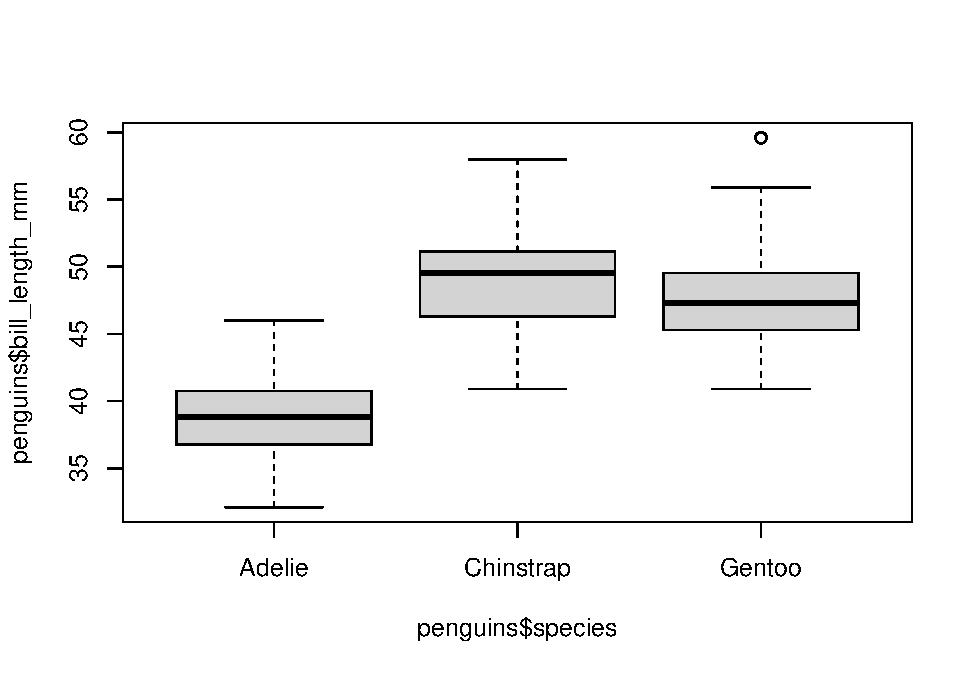
\includegraphics{_main_files/figure-latex/anova-1.pdf}

\begin{Shaded}
\begin{Highlighting}[]
\NormalTok{model.spp <-}\StringTok{ }\KeywordTok{aov}\NormalTok{(bill_length_mm }\OperatorTok{~}\StringTok{ }\NormalTok{species, }\DataTypeTok{data =} \KeywordTok{na.omit}\NormalTok{(penguins))}
\KeywordTok{summary}\NormalTok{(model.spp)}
\end{Highlighting}
\end{Shaded}

\begin{verbatim}
##              Df Sum Sq Mean Sq F value Pr(>F)    
## species       2   7015    3508   397.3 <2e-16 ***
## Residuals   330   2914       9                   
## ---
## Signif. codes:  0 '***' 0.001 '**' 0.01 '*' 0.05 '.' 0.1 ' ' 1
\end{verbatim}

\begin{Shaded}
\begin{Highlighting}[]
\KeywordTok{summary}\NormalTok{(}\KeywordTok{lm}\NormalTok{(bill_length_mm }\OperatorTok{~}\StringTok{ }\NormalTok{species, }\DataTypeTok{data =} \KeywordTok{na.omit}\NormalTok{(penguins)))}
\end{Highlighting}
\end{Shaded}

\begin{verbatim}
## 
## Call:
## lm(formula = bill_length_mm ~ species, data = na.omit(penguins))
## 
## Residuals:
##    Min     1Q Median     3Q    Max 
## -7.934 -2.234  0.076  2.066 12.032 
## 
## Coefficients:
##                  Estimate Std. Error t value Pr(>|t|)    
## (Intercept)       38.8240     0.2459  157.88   <2e-16 ***
## speciesChinstrap  10.0099     0.4362   22.95   <2e-16 ***
## speciesGentoo      8.7441     0.3670   23.83   <2e-16 ***
## ---
## Signif. codes:  0 '***' 0.001 '**' 0.01 '*' 0.05 '.' 0.1 ' ' 1
## 
## Residual standard error: 2.971 on 330 degrees of freedom
## Multiple R-squared:  0.7066, Adjusted R-squared:  0.7048 
## F-statistic: 397.3 on 2 and 330 DF,  p-value: < 2.2e-16
\end{verbatim}

\begin{Shaded}
\begin{Highlighting}[]
\CommentTok{# Comparaciones multiples}
\KeywordTok{TukeyHSD}\NormalTok{(model.spp)}
\end{Highlighting}
\end{Shaded}

\begin{verbatim}
##   Tukey multiple comparisons of means
##     95% family-wise confidence level
## 
## Fit: aov(formula = bill_length_mm ~ species, data = na.omit(penguins))
## 
## $species
##                       diff       lwr        upr     p adj
## Chinstrap-Adelie 10.009851  8.982789 11.0369128 0.0000000
## Gentoo-Adelie     8.744095  7.880135  9.6080546 0.0000000
## Gentoo-Chinstrap -1.265756 -2.329197 -0.2023151 0.0148212
\end{verbatim}

\hypertarget{supuestos}{%
\section{Supuestos}\label{supuestos}}

\hypertarget{colinealidad}{%
\subsection{Colinealidad}\label{colinealidad}}

\begin{Shaded}
\begin{Highlighting}[]
\KeywordTok{library}\NormalTok{(car)}
\end{Highlighting}
\end{Shaded}

\begin{verbatim}
## Loading required package: carData
\end{verbatim}

\begin{verbatim}
## Registered S3 methods overwritten by 'car':
##   method                          from
##   influence.merMod                lme4
##   cooks.distance.influence.merMod lme4
##   dfbeta.influence.merMod         lme4
##   dfbetas.influence.merMod        lme4
\end{verbatim}

\begin{verbatim}
## 
## Attaching package: 'car'
\end{verbatim}

\begin{verbatim}
## The following object is masked from 'package:psych':
## 
##     logit
\end{verbatim}

\begin{Shaded}
\begin{Highlighting}[]
\KeywordTok{vif}\NormalTok{(model.Ad)}
\end{Highlighting}
\end{Shaded}

\begin{verbatim}
##   body_mass_g bill_depth_mm 
##      1.496861      1.496861
\end{verbatim}

\hypertarget{anuxe1lisis-de-residuos}{%
\subsection{Análisis de residuos}\label{anuxe1lisis-de-residuos}}

\begin{Shaded}
\begin{Highlighting}[]
\CommentTok{# Regresión}
\KeywordTok{hist}\NormalTok{(model.Ad}\OperatorTok{$}\NormalTok{residuals)}
\end{Highlighting}
\end{Shaded}

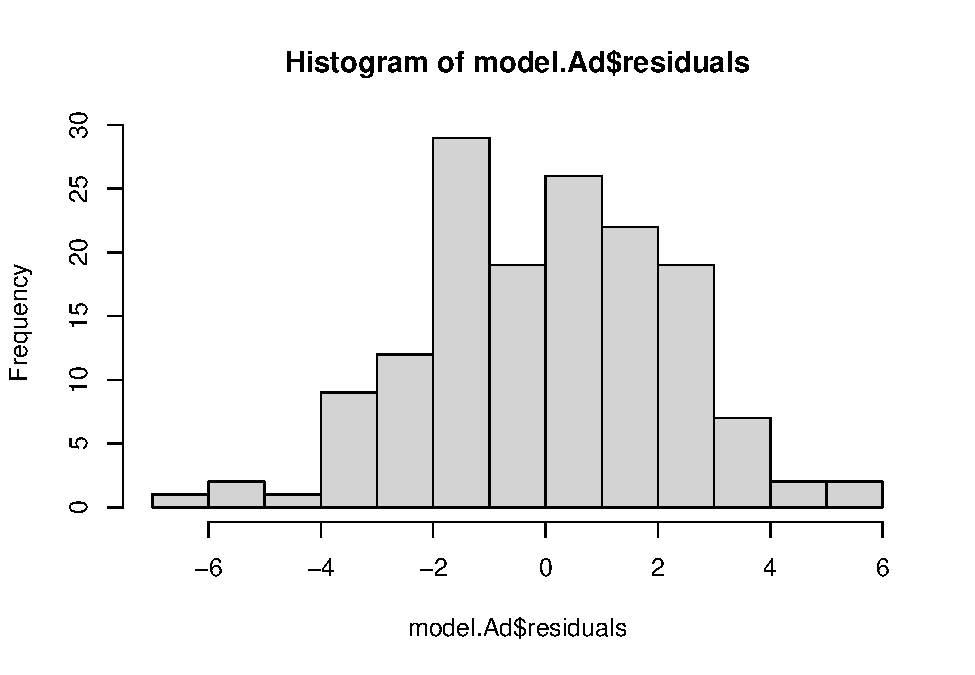
\includegraphics{_main_files/figure-latex/residuos-1.pdf}

\begin{Shaded}
\begin{Highlighting}[]
\KeywordTok{qqPlot}\NormalTok{(model.Ad}\OperatorTok{$}\NormalTok{residuals)}
\end{Highlighting}
\end{Shaded}

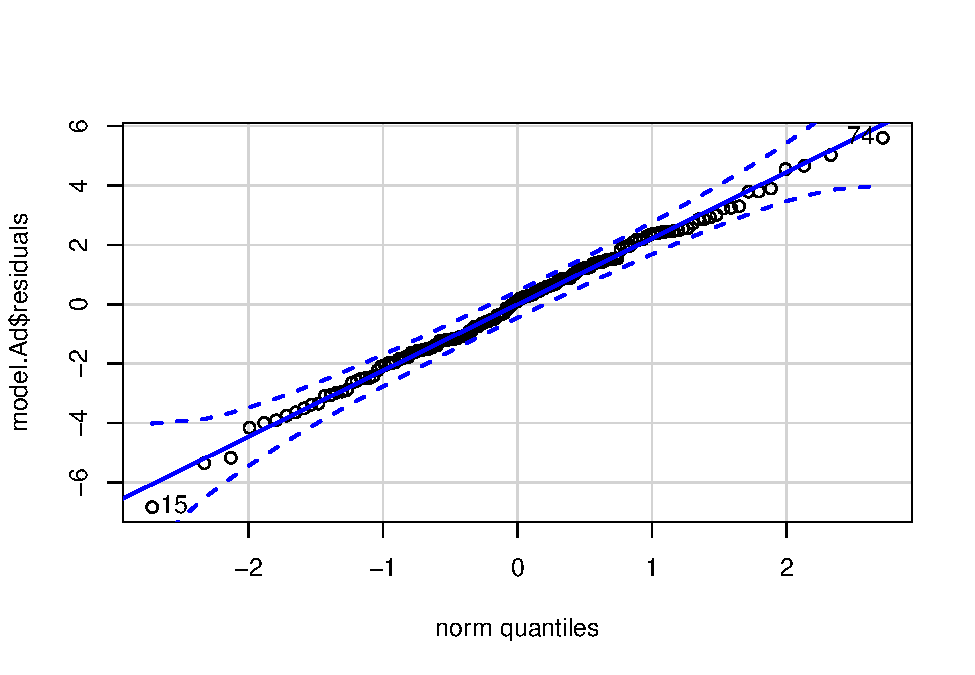
\includegraphics{_main_files/figure-latex/residuos-2.pdf}

\begin{verbatim}
## 15 74 
## 14 73
\end{verbatim}

\begin{Shaded}
\begin{Highlighting}[]
\KeywordTok{layout}\NormalTok{(}\KeywordTok{matrix}\NormalTok{(}\DecValTok{1}\OperatorTok{:}\DecValTok{4}\NormalTok{, }\DecValTok{2}\NormalTok{, }\DecValTok{2}\NormalTok{))}
\KeywordTok{plot}\NormalTok{(model.Ad)}
\end{Highlighting}
\end{Shaded}

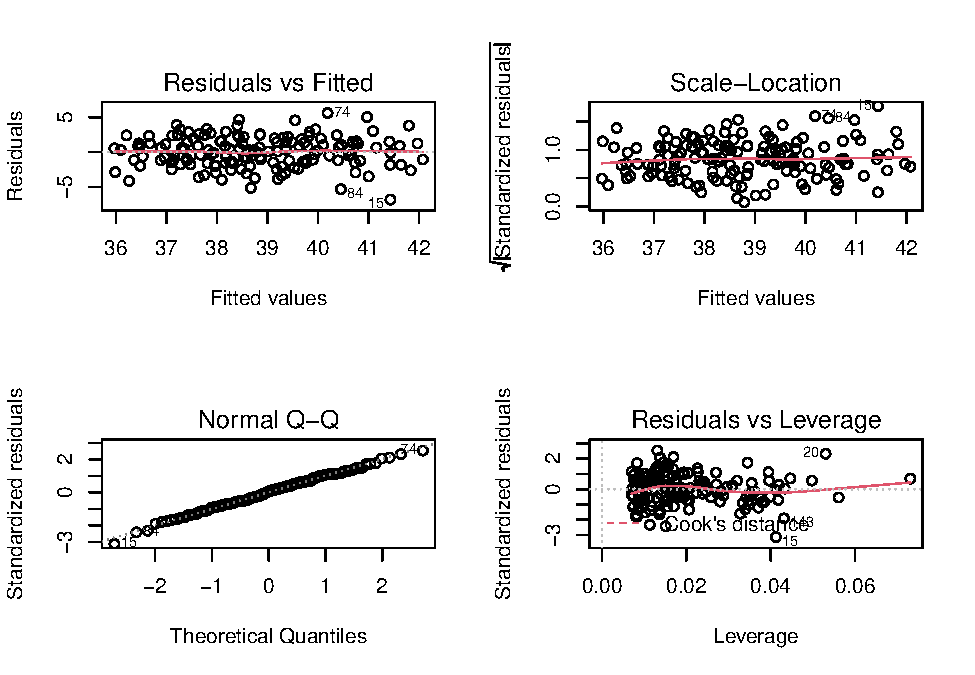
\includegraphics{_main_files/figure-latex/residuos-3.pdf}

\begin{Shaded}
\begin{Highlighting}[]
\KeywordTok{layout}\NormalTok{(}\DecValTok{1}\NormalTok{)}

\CommentTok{# Test de t y ANOVA}
\NormalTok{model.spp <-}\StringTok{ }\KeywordTok{aov}\NormalTok{(bill_length_mm }\OperatorTok{~}\StringTok{ }\NormalTok{species, }\DataTypeTok{data =} \KeywordTok{na.omit}\NormalTok{(penguins))}
\NormalTok{resid.model.spp <-}\StringTok{ }\KeywordTok{resid}\NormalTok{(model.spp)}
\KeywordTok{boxplot}\NormalTok{(resid.model.spp }\OperatorTok{~}\StringTok{ }\NormalTok{species, }\DataTypeTok{data =} \KeywordTok{na.omit}\NormalTok{(penguins)) }
\end{Highlighting}
\end{Shaded}

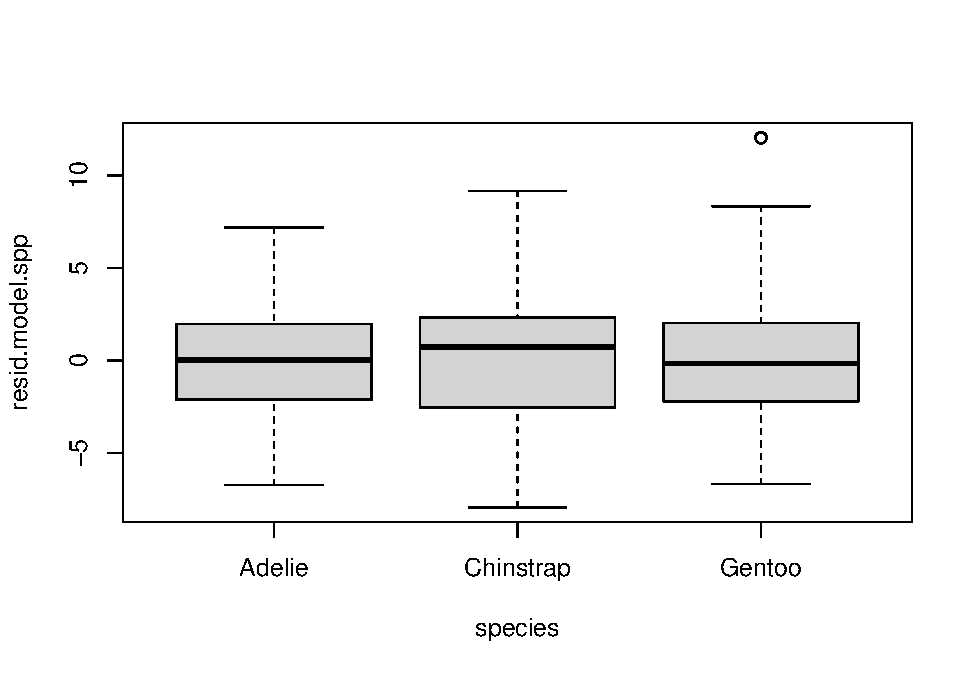
\includegraphics{_main_files/figure-latex/residuos-4.pdf}

\begin{Shaded}
\begin{Highlighting}[]
\KeywordTok{termplot}\NormalTok{(model.spp, }\DataTypeTok{se =} \OtherTok{TRUE}\NormalTok{, }\DataTypeTok{partial.resid =} \OtherTok{TRUE}\NormalTok{)}
\end{Highlighting}
\end{Shaded}

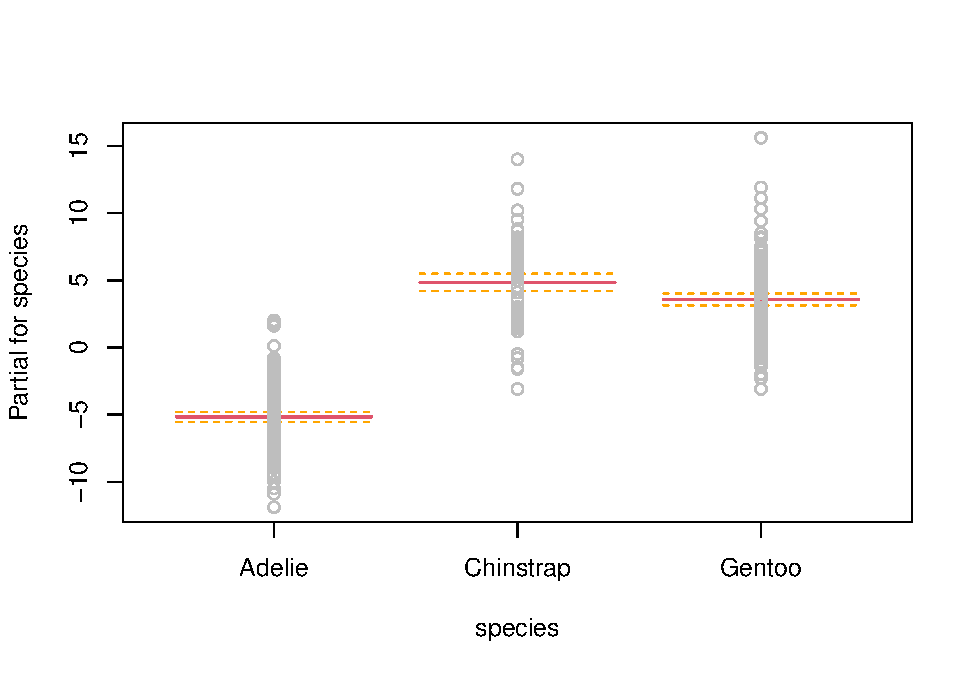
\includegraphics{_main_files/figure-latex/residuos-5.pdf}

\begin{Shaded}
\begin{Highlighting}[]
\KeywordTok{bartlett.test}\NormalTok{(resid.model.spp }\OperatorTok{~}\StringTok{ }\NormalTok{species, }\DataTypeTok{data =} \KeywordTok{na.omit}\NormalTok{(penguins)) }
\end{Highlighting}
\end{Shaded}

\begin{verbatim}
## 
##  Bartlett test of homogeneity of variances
## 
## data:  resid.model.spp by species
## Bartlett's K-squared = 5.6782, df = 2, p-value = 0.05848
\end{verbatim}

\hypertarget{transformaciones}{%
\section{Transformaciones}\label{transformaciones}}

\[log(y) = y' = \beta_0 + \beta_1 x_1 + \beta_2 x_2 + ... + \beta_n x_n + \epsilon\]

\begin{Shaded}
\begin{Highlighting}[]
\KeywordTok{layout}\NormalTok{(}\KeywordTok{matrix}\NormalTok{(}\DecValTok{1}\OperatorTok{:}\DecValTok{6}\NormalTok{, }\DecValTok{2}\NormalTok{, }\DecValTok{3}\NormalTok{))}
\NormalTok{abundancia <-}\StringTok{ }\KeywordTok{rpois}\NormalTok{(}\DataTypeTok{n =} \DecValTok{1000}\NormalTok{, }\DataTypeTok{lambda =} \DecValTok{4}\NormalTok{)}
\KeywordTok{hist}\NormalTok{(abundancia, }\DataTypeTok{main =} \StringTok{"Abundancia"}\NormalTok{)}
\NormalTok{log.abun <-}\StringTok{ }\KeywordTok{log}\NormalTok{(abundancia }\OperatorTok{+}\StringTok{ }\DecValTok{1}\NormalTok{)}
\KeywordTok{hist}\NormalTok{(log.abun, }\DataTypeTok{breaks =} \DecValTok{6}\NormalTok{, }\DataTypeTok{main =} \StringTok{"log(Abundancia + 1)"}\NormalTok{)}

\NormalTok{peso <-}\StringTok{ }\KeywordTok{rgamma}\NormalTok{(}\DataTypeTok{n =} \DecValTok{1000}\NormalTok{, }\DataTypeTok{shape =} \DecValTok{5}\NormalTok{)}
\KeywordTok{hist}\NormalTok{(peso, }\DataTypeTok{main =} \StringTok{"Peso"}\NormalTok{)}
\NormalTok{sqrt.peso <-}\StringTok{ }\KeywordTok{sqrt}\NormalTok{(peso)}
\KeywordTok{hist}\NormalTok{(sqrt.peso, }\DataTypeTok{breaks =} \DecValTok{6}\NormalTok{, }\DataTypeTok{main =} \StringTok{"Raíz cuadrada del peso"}\NormalTok{)}

\NormalTok{prop.infectados <-}\StringTok{ }\KeywordTok{rbinom}\NormalTok{(}\DataTypeTok{n =} \DecValTok{1000}\NormalTok{, }\DataTypeTok{size =} \DecValTok{10}\NormalTok{, }\DataTypeTok{p =} \FloatTok{0.4}\NormalTok{)}\OperatorTok{/}\DecValTok{10}
\KeywordTok{hist}\NormalTok{(prop.infectados, }\DataTypeTok{main =} \StringTok{"Proporción de infectados"}\NormalTok{)}
\NormalTok{logit.prop <-}\StringTok{ }\KeywordTok{log}\NormalTok{(prop.infectados}\OperatorTok{/}\NormalTok{(}\DecValTok{1} \OperatorTok{-}\StringTok{ }\NormalTok{prop.infectados))}
\KeywordTok{hist}\NormalTok{(logit.prop, }\DataTypeTok{main =} \StringTok{"Logit proporción de infectados"}\NormalTok{, }\DataTypeTok{breaks =} \DecValTok{6}\NormalTok{)}
\end{Highlighting}
\end{Shaded}

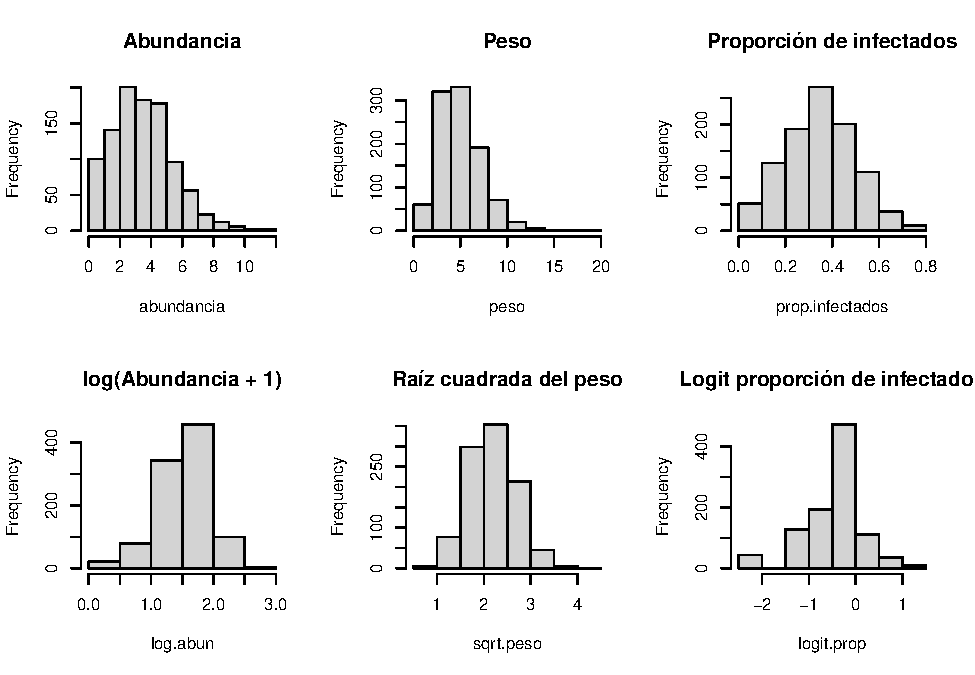
\includegraphics{_main_files/figure-latex/transformaciones-1.pdf}

\begin{Shaded}
\begin{Highlighting}[]
\KeywordTok{layout}\NormalTok{(}\DecValTok{1}\NormalTok{)}
\end{Highlighting}
\end{Shaded}

\hypertarget{actividades}{%
\section{Actividades}\label{actividades}}

\hypertarget{ejercicios-de-repaso}{%
\subsection{Ejercicios de repaso}\label{ejercicios-de-repaso}}

1.1. Calcule:

\begin{itemize}
\item
  El logaritmo en base e y en base 10 de 9.
\item
  La raíz cuadrada y quinta de 10.
\end{itemize}

1.2. Genere los siguientes vectores x e y, respectivamente:

1 4 7 11 5 2
1 2 3 4 5 6

Luego, identifique las operaciones para obtener:

2 6 10 15 10 8
2 8 14 22 10 4
3 6 9 12 15 18

1.3. Genere las siguientes secuencias:

1 2 3 4 5 6 7 8 9 10 11
5 6 7 8 9 10
5.0 5.5 6.0 6.5 7.0 7.5 8.0 8.5 9.0 9.5 10.0
10.0 10.1 10.2 10.3 10.4 10.5 10.6 10.7 10.8 10.9 11.0 11.1 11.2 11.3
1 3 5 7 9
9 7 5 3 1
3 3 3 3 3
1 2 1 2 1 2 1 2 1 2
``IML'' ``R'' ``IML'' ``R'' ``IML'' ``R'' ``IML'' ``R''
1 1 1 2 2 2 3 3 3 4 4 4 5 5 5

1.4. Cree un vector que represente una variable aleatoria de 1000 valores con distribución normal estándar.

\begin{itemize}
\item
  Grafique un histograma (color naranja), teniendo en cuenta 10 y 15 celdas.
\item
  Calcule su media y desvío estándar.
\item
  Calcule qué porcentaje de los datos se encuentra entre 2 desvíos estándares.
\end{itemize}

1.5. Cree un vector que represente una variable aleatoria de 500 valores con distribución de Poisson y diferentes medias (1, 5 y 100).

\begin{itemize}
\item
  Para cada distribución, calcule su media y varianza.
\item
  Grafique los tres histogramas en el mismo panel ¿Qué observa?
\item
  Haga una tabla que muestre la frecuencia para cada conteo y luego realice un gráfico de barras.
\end{itemize}

1.6. Utilizando la variable aleatoria del Ejercicio 1.2, construya un marco de datos que incluya además, un factor de 4 niveles con el mismo número de observaciones en cada nivel, de tal forma que los primeros valores pertenezcan al primer nivel, los siguientes al segundo nivel y así sucesivamente.

\begin{itemize}
\tightlist
\item
  Calcule la media y desvío estándar para los valores de cada nivel, y luego grafique un histograma para cada uno de ellos.
\end{itemize}

1.7. A partir de información de la web, construya un marco de datos que incluya como variables 5 ciudades del mundo, con su área y número de habitantes.

\begin{itemize}
\item
  Obtenga cuál es la ciudad con el mayor número de habitantes de su marco de datos y en qué fila se encuentra.
\item
  Filtre aquellas ciudades con más de 500 mil habitantes.
\item
  Filtre aquellas ciudades con menos de 300 mil habitantes y un área menor a 250 mil ha.
\item
  Cree una columna adicional binaria, en la cual a aquellas ciudades con más de 500 mil habitantes se le asigne un 1, o de lo contrario, un 0.
\end{itemize}

1.8. Simule 1000 valores de una distribución normal (media = 10, desvío = 3) y utilicela como predictor en un modelo de regresión lineal, de forma tal que la variable respuesta cambie 0.2 unidades por unidad del predictor.

\begin{itemize}
\item
  Calcule la covarianza y la correlación de Pearson entre ambas variables.
\item
  Grafique un diagrama de dispersión junto con el modelo ajustado.
\item
  Realice un resumen del modelo y compare las estimaciones de los parámetros obtenidos (intercepto, pendiente y varianza de los residuos) con los poblacionales.
\item
  Estandarice ambas variables y calcule la correlación de Pearson ¿Qué observa y por qué?
\item
  Con los mismos parámetros, simule ahora 50 valores y obtenga el resumen del modelo ¿Qué sucede con la pendiente y la significancia, y por qué?
\end{itemize}

\hypertarget{ejercicio-1.2}{%
\subsection{Ejercicio 1.2}\label{ejercicio-1.2}}

Se analizó la diversidad de diatomeas (\texttt{div}) en cursos de agua (\texttt{curso}) con distintos niveles de concentración de zinc (\texttt{zinc}). Los datos se encuentran en el archivo \texttt{diatom.xls}. Grafique la distribución de frecuencias de la diversidad de diatomeas y la diversidad como función de la concentración de zinc. Calcule la media, mediana, varianza, desvío estándar y coeficiente de variación de la diversidad para cada concentración de zinc ¿Qué patrón le sugieren los datos?

\hypertarget{ejercicio-1.3}{%
\subsection{Ejercicio 1.3}\label{ejercicio-1.3}}

Sokal \& Rohlf (1997) analizaron el consumo de oxígeno en dos especies de lapas bajo tres concentraciones de agua de mar (\texttt{limpets.csv}).

\begin{itemize}
\item
  Calcule la media y varianza para cada especie, concentración y combinación de especie y concentración.
\item
  Realice un gráfico que muestre las diferentes combinaciones entre especie y concentración. Grafique e interprete la interacción entre ambos factores utilizando la función \texttt{interaction.plot} del paquete \texttt{car}.
\item
  ¿Existen diferencias entre las especies y las concentraciones? Utilice un modelo adecuado que responda a esta pregunta.
\item
  Evalúe los supuestos del modelo.
\end{itemize}

\hypertarget{ejercicio-1.4}{%
\subsection{Ejercicio 1.4}\label{ejercicio-1.4}}

Allison \& Cicchetti (1976) compilaron la cantidad de horas de sueño, la morfología y el riesgo de predación (escala de 1 a 5 -menor valor, menor riesgo de predación-) en 62 especies de mamíferos (\texttt{allison.csv}).

\begin{itemize}
\item
  Realice un resumen (media, desvío y coeficiente de variación) de las variables del conjunto de datos.
\item
  Grafique histogramas para cada una de las variables y diagramas de dispersión para cada par de variables.
\item
  Ajuste un modelo adecuado entre longevidad en años (\texttt{LifeSpan}), masa corporal en kg (\texttt{BodyWt}) y predación (\texttt{Predation}).
\item
  Grafique la relación entre masa corporal y longevidad, para cada nivel de predación ¿Puede observar algún patrón que haga reconsiderar el modelo ajustado en el inciso anterior?
\item
  Evalúe los supuestos del modelo final.
\item
  Realice un gráfico que represente el modelo ajustado.
\item
  Según el modelo ¿Cuánto sería la longevidad para el ser humano, bajo los supuestos que considere? ¿Es realista la predicción que obtuvo?
\end{itemize}

\hypertarget{modelos-lineales-generalizados}{%
\chapter{Modelos lineales generalizados}\label{modelos-lineales-generalizados}}

\hypertarget{datos-de-presencia-ausencia}{%
\section{Datos de presencia-ausencia}\label{datos-de-presencia-ausencia}}

Cabral et al.~(2007) estudiaron la distribución de platijas (\emph{Solea solea}) en el estuario Tagus, Portugal (\texttt{Solea.txt}). Se desea saber qué factores (temperatura, transparencia, salinidad) están relacionados con la presencia esta especie.

\begin{Shaded}
\begin{Highlighting}[]
\CommentTok{# Analisis exploratorio}
\NormalTok{datos <-}\StringTok{ }\KeywordTok{read.table}\NormalTok{(}\StringTok{"Solea.txt"}\NormalTok{, }\DataTypeTok{header =} \OtherTok{TRUE}\NormalTok{)}
\KeywordTok{str}\NormalTok{(datos)}
\end{Highlighting}
\end{Shaded}

\begin{verbatim}
## 'data.frame':    65 obs. of  13 variables:
##  $ Sample       : int  1 2 3 4 5 6 7 8 9 10 ...
##  $ season       : int  1 1 1 1 1 1 1 1 1 1 ...
##  $ month        : int  5 5 5 5 5 5 5 5 5 5 ...
##  $ Area         : int  2 2 2 4 4 4 3 3 3 1 ...
##  $ depth        : num  3 2.6 2.6 2.1 3.2 3.5 1.6 1.7 1.8 4.5 ...
##  $ temperature  : int  20 18 19 20 20 20 19 17 19 21 ...
##  $ salinity     : int  30 29 30 29 30 32 29 28 29 12 ...
##  $ transparency : int  15 15 15 15 15 7 15 10 10 35 ...
##  $ gravel       : num  3.74 1.94 2.88 11.06 9.87 ...
##  $ large_sand   : num  13.15 4.99 8.98 11.96 28.6 ...
##  $ med_fine_sand: num  11.93 5.43 16.85 21.95 19.49 ...
##  $ mud          : num  71.2 87.6 71.3 55 42 ...
##  $ Solea_solea  : int  0 0 1 0 0 0 1 1 0 1 ...
\end{verbatim}

\begin{Shaded}
\begin{Highlighting}[]
\KeywordTok{hist}\NormalTok{(datos}\OperatorTok{$}\NormalTok{Solea_solea)}
\end{Highlighting}
\end{Shaded}

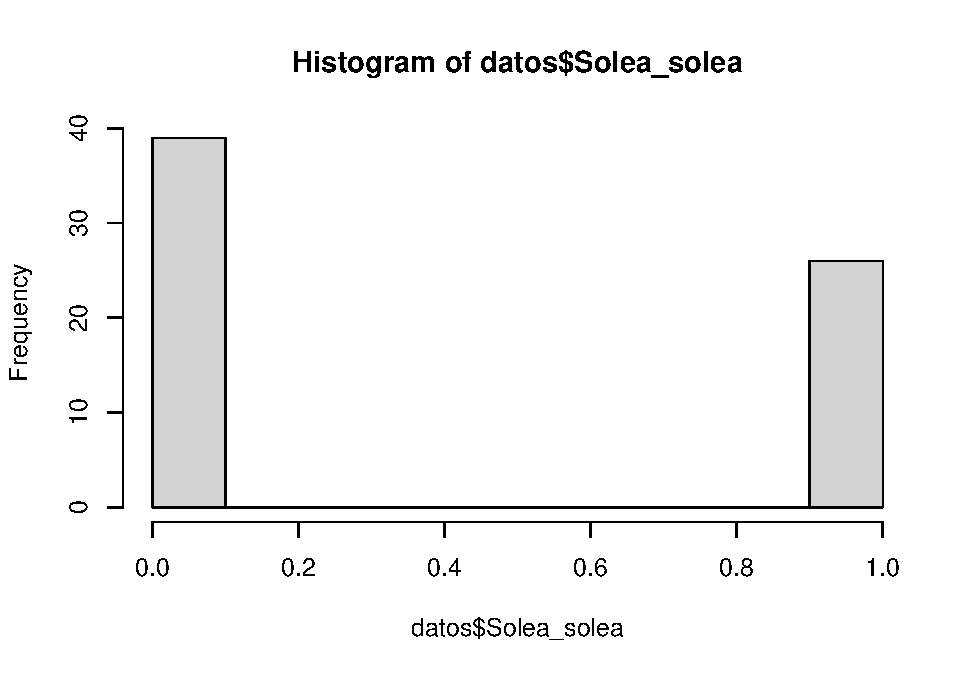
\includegraphics{_main_files/figure-latex/explo1-1.pdf}

\begin{Shaded}
\begin{Highlighting}[]
\KeywordTok{table}\NormalTok{(datos}\OperatorTok{$}\NormalTok{Solea_solea)}
\end{Highlighting}
\end{Shaded}

\begin{verbatim}
## 
##  0  1 
## 39 26
\end{verbatim}

\begin{Shaded}
\begin{Highlighting}[]
\KeywordTok{pairs}\NormalTok{(datos[, }\DecValTok{4}\OperatorTok{:}\DecValTok{12}\NormalTok{])}
\end{Highlighting}
\end{Shaded}

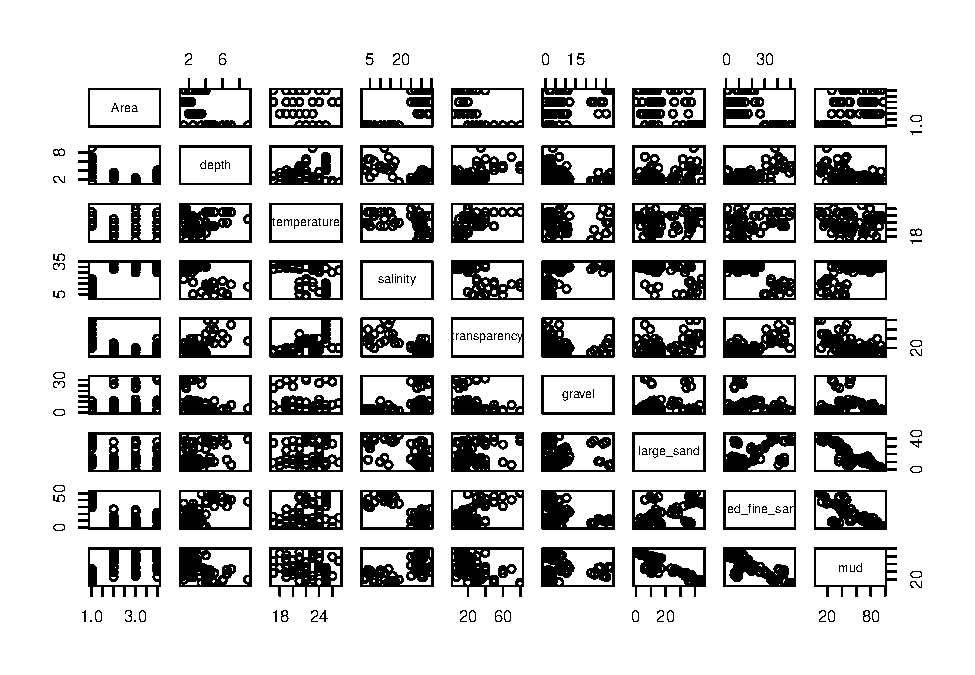
\includegraphics{_main_files/figure-latex/explo1-2.pdf}

\begin{Shaded}
\begin{Highlighting}[]
\KeywordTok{round}\NormalTok{(}\KeywordTok{cor}\NormalTok{(datos[, }\DecValTok{4}\OperatorTok{:}\DecValTok{12}\NormalTok{]), }\DecValTok{2}\NormalTok{)}
\end{Highlighting}
\end{Shaded}

\begin{verbatim}
##                Area depth temperature salinity transparency gravel large_sand
## Area           1.00 -0.55       -0.18     0.76        -0.56   0.44      -0.44
## depth         -0.55  1.00        0.14    -0.66         0.57  -0.24       0.31
## temperature   -0.18  0.14        1.00    -0.35         0.54  -0.16       0.12
## salinity       0.76 -0.66       -0.35     1.00        -0.66   0.38      -0.54
## transparency  -0.56  0.57        0.54    -0.66         1.00  -0.25       0.37
## gravel         0.44 -0.24       -0.16     0.38        -0.25   1.00       0.01
## large_sand    -0.44  0.31        0.12    -0.54         0.37   0.01       1.00
## med_fine_sand -0.69  0.67        0.25    -0.80         0.69  -0.32       0.56
## mud            0.49 -0.47       -0.16     0.63        -0.52  -0.19      -0.87
##               med_fine_sand   mud
## Area                  -0.69  0.49
## depth                  0.67 -0.47
## temperature            0.25 -0.16
## salinity              -0.80  0.63
## transparency           0.69 -0.52
## gravel                -0.32 -0.19
## large_sand             0.56 -0.87
## med_fine_sand          1.00 -0.78
## mud                   -0.78  1.00
\end{verbatim}

\hypertarget{glm-binomial}{%
\subsection{GLM binomial}\label{glm-binomial}}

\begin{Shaded}
\begin{Highlighting}[]
\NormalTok{m.bin <-}\StringTok{ }\KeywordTok{glm}\NormalTok{(Solea_solea }\OperatorTok{~}\StringTok{ }\NormalTok{temperature }\OperatorTok{+}\StringTok{ }\NormalTok{transparency }\OperatorTok{+}\StringTok{ }\NormalTok{salinity, }\DataTypeTok{family =}\NormalTok{ binomial, }\DataTypeTok{data =}\NormalTok{ datos)}
\KeywordTok{summary}\NormalTok{(m.bin)}
\end{Highlighting}
\end{Shaded}

\begin{verbatim}
## 
## Call:
## glm(formula = Solea_solea ~ temperature + transparency + salinity, 
##     family = binomial, data = datos)
## 
## Deviance Residuals: 
##     Min       1Q   Median       3Q      Max  
## -2.2170  -0.7607  -0.6364   0.7219   1.8447  
## 
## Coefficients:
##               Estimate Std. Error z value Pr(>|z|)   
## (Intercept)   5.221629   3.524358   1.482  0.13845   
## temperature  -0.100542   0.148829  -0.676  0.49932   
## transparency -0.001162   0.025347  -0.046  0.96343   
## salinity     -0.142652   0.049986  -2.854  0.00432 **
## ---
## Signif. codes:  0 '***' 0.001 '**' 0.01 '*' 0.05 '.' 0.1 ' ' 1
## 
## (Dispersion parameter for binomial family taken to be 1)
## 
##     Null deviance: 87.492  on 64  degrees of freedom
## Residual deviance: 67.973  on 61  degrees of freedom
## AIC: 75.973
## 
## Number of Fisher Scoring iterations: 4
\end{verbatim}

\hypertarget{diagnuxf3sticos}{%
\subsection{Diagnósticos}\label{diagnuxf3sticos}}

\begin{Shaded}
\begin{Highlighting}[]
\KeywordTok{plot}\NormalTok{(m.bin)}
\end{Highlighting}
\end{Shaded}

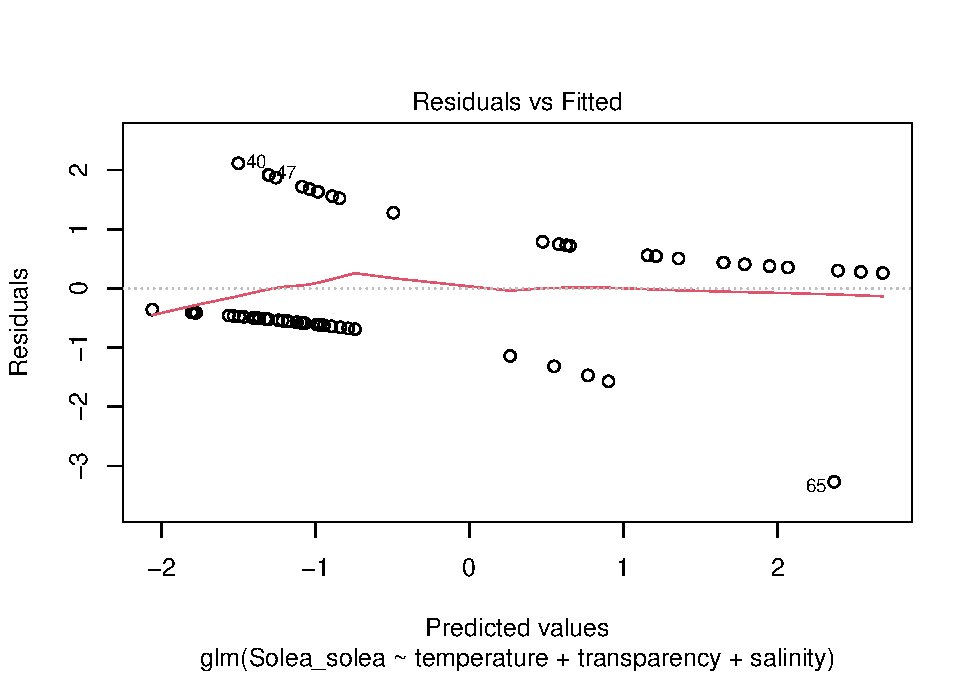
\includegraphics{_main_files/figure-latex/validacion glm binomial-1.pdf} 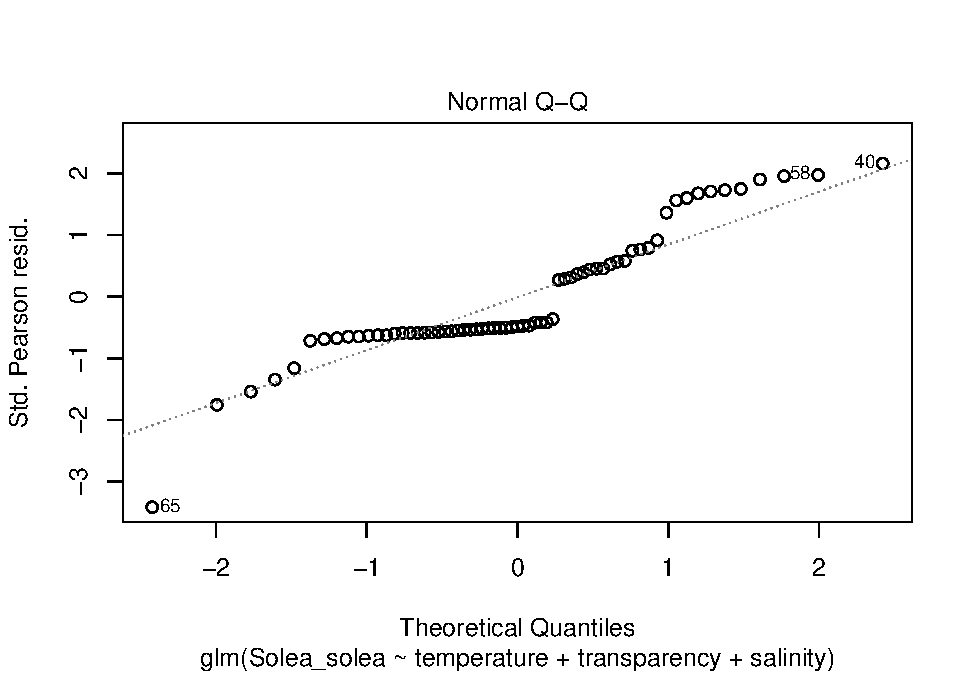
\includegraphics{_main_files/figure-latex/validacion glm binomial-2.pdf} 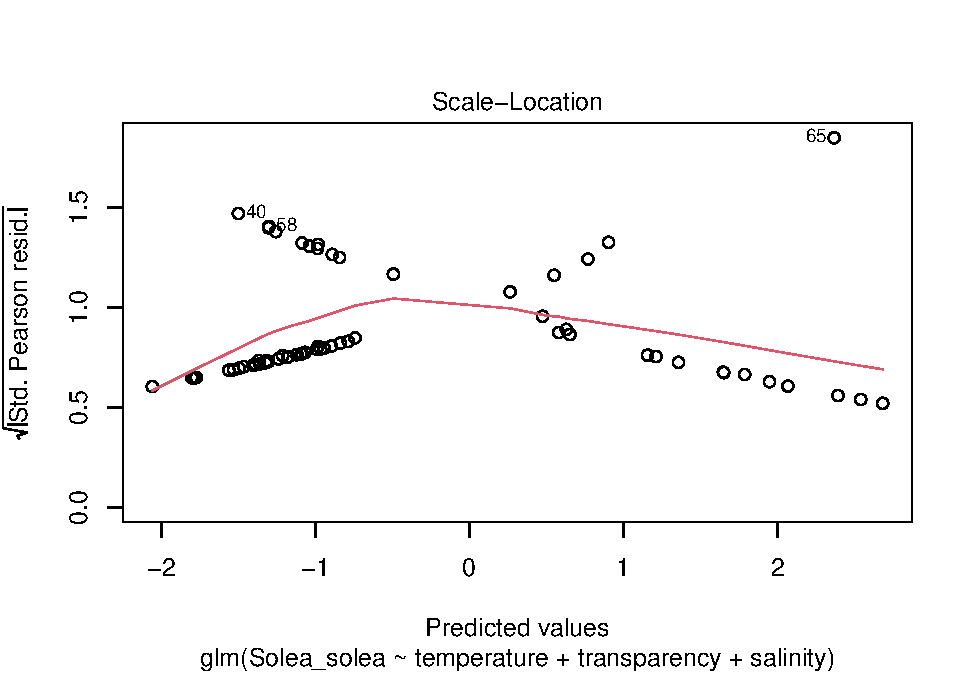
\includegraphics{_main_files/figure-latex/validacion glm binomial-3.pdf} 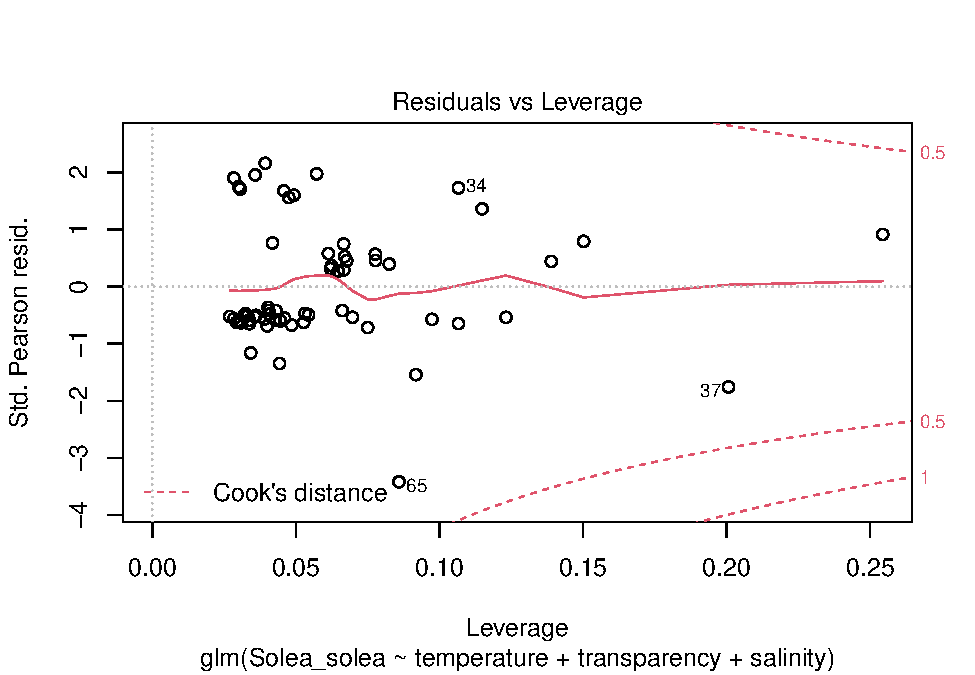
\includegraphics{_main_files/figure-latex/validacion glm binomial-4.pdf}

\begin{Shaded}
\begin{Highlighting}[]
\KeywordTok{library}\NormalTok{(DHARMa)}
\end{Highlighting}
\end{Shaded}

\begin{verbatim}
## Warning: package 'DHARMa' was built under R version 4.0.5
\end{verbatim}

\begin{verbatim}
## This is DHARMa 0.4.5. For overview type '?DHARMa'. For recent changes, type news(package = 'DHARMa')
\end{verbatim}

\begin{Shaded}
\begin{Highlighting}[]
\KeywordTok{plot}\NormalTok{(}\KeywordTok{simulateResiduals}\NormalTok{(}\DataTypeTok{fittedModel =}\NormalTok{ m.bin))}
\end{Highlighting}
\end{Shaded}

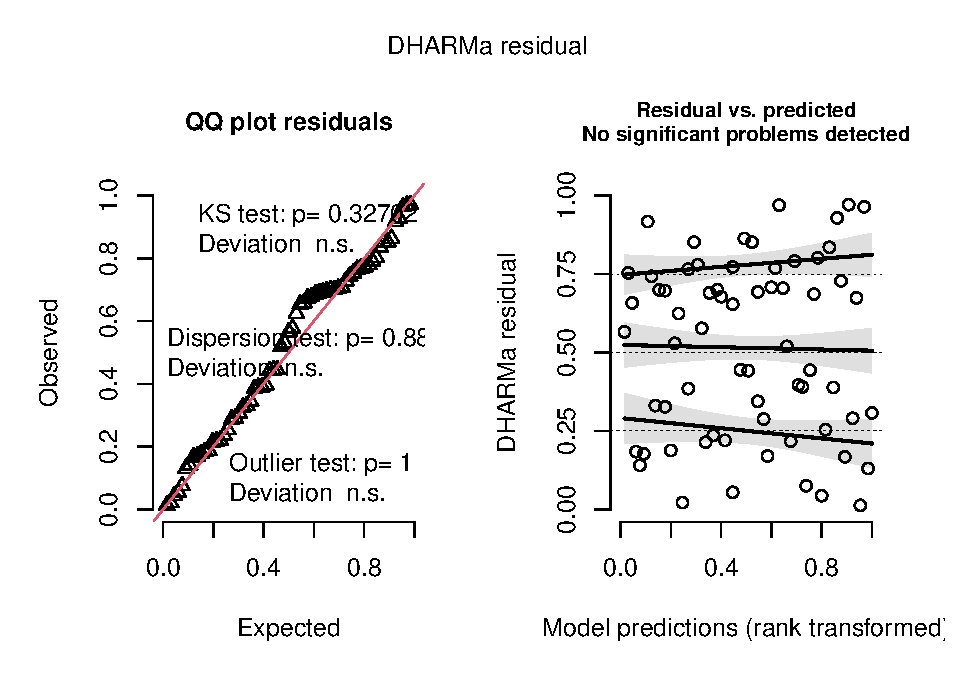
\includegraphics{_main_files/figure-latex/validacion glm binomial-5.pdf}

\hypertarget{bondad-del-ajuste}{%
\subsection{Bondad del ajuste}\label{bondad-del-ajuste}}

\begin{Shaded}
\begin{Highlighting}[]
\KeywordTok{summary}\NormalTok{(m.bin)}
\end{Highlighting}
\end{Shaded}

\begin{verbatim}
## 
## Call:
## glm(formula = Solea_solea ~ temperature + transparency + salinity, 
##     family = binomial, data = datos)
## 
## Deviance Residuals: 
##     Min       1Q   Median       3Q      Max  
## -2.2170  -0.7607  -0.6364   0.7219   1.8447  
## 
## Coefficients:
##               Estimate Std. Error z value Pr(>|z|)   
## (Intercept)   5.221629   3.524358   1.482  0.13845   
## temperature  -0.100542   0.148829  -0.676  0.49932   
## transparency -0.001162   0.025347  -0.046  0.96343   
## salinity     -0.142652   0.049986  -2.854  0.00432 **
## ---
## Signif. codes:  0 '***' 0.001 '**' 0.01 '*' 0.05 '.' 0.1 ' ' 1
## 
## (Dispersion parameter for binomial family taken to be 1)
## 
##     Null deviance: 87.492  on 64  degrees of freedom
## Residual deviance: 67.973  on 61  degrees of freedom
## AIC: 75.973
## 
## Number of Fisher Scoring iterations: 4
\end{verbatim}

\begin{Shaded}
\begin{Highlighting}[]
\CommentTok{# Pseudo-R2}
\DecValTok{1} \OperatorTok{-}\StringTok{ }\NormalTok{(m.bin}\OperatorTok{$}\NormalTok{dev}\OperatorTok{/}\NormalTok{m.bin}\OperatorTok{$}\NormalTok{null)}
\end{Highlighting}
\end{Shaded}

\begin{verbatim}
## [1] 0.2230856
\end{verbatim}

\begin{Shaded}
\begin{Highlighting}[]
\KeywordTok{library}\NormalTok{(performance)}
\end{Highlighting}
\end{Shaded}

\begin{verbatim}
## Warning: package 'performance' was built under R version 4.0.5
\end{verbatim}

\begin{Shaded}
\begin{Highlighting}[]
\CommentTok{# Coeficiente de determinación de Tjur}
\KeywordTok{r2_tjur}\NormalTok{(m.bin) }
\end{Highlighting}
\end{Shaded}

\begin{verbatim}
## Tjur's R2 
## 0.2840808
\end{verbatim}

\hypertarget{gruxe1fico-del-modelo}{%
\subsection{Gráfico del modelo}\label{gruxe1fico-del-modelo}}

\begin{Shaded}
\begin{Highlighting}[]
\KeywordTok{library}\NormalTok{(visreg)}
\KeywordTok{visreg}\NormalTok{(}\DataTypeTok{fit =}\NormalTok{ m.bin, }\DataTypeTok{xvar =} \StringTok{"salinity"}\NormalTok{, }\DataTypeTok{scale =} \StringTok{"response"}\NormalTok{, }\DataTypeTok{ylim =} \KeywordTok{c}\NormalTok{(}\DecValTok{0}\NormalTok{, }\DecValTok{1}\NormalTok{), }
       \DataTypeTok{xlab =} \StringTok{"Salinidad"}\NormalTok{, }\DataTypeTok{ylab =} \StringTok{"Probabilidad de presencia"}\NormalTok{) }
\KeywordTok{points}\NormalTok{(datos}\OperatorTok{$}\NormalTok{salinity, datos}\OperatorTok{$}\NormalTok{Solea_solea)}
\end{Highlighting}
\end{Shaded}

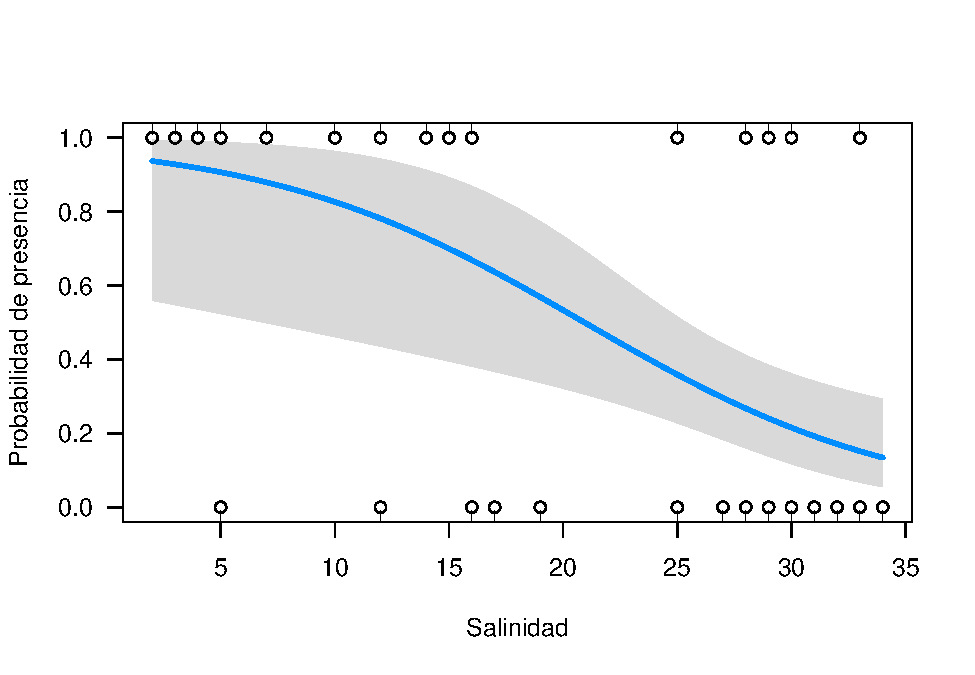
\includegraphics{_main_files/figure-latex/grafico binomial-1.pdf}

\hypertarget{interpretaciuxf3n-de-los-coeficientes}{%
\subsection{Interpretación de los coeficientes}\label{interpretaciuxf3n-de-los-coeficientes}}

\begin{Shaded}
\begin{Highlighting}[]
\KeywordTok{exp}\NormalTok{(m.bin}\OperatorTok{$}\NormalTok{coeff[}\DecValTok{2}\NormalTok{]) }\CommentTok{# Razon de odds}
\end{Highlighting}
\end{Shaded}

\begin{verbatim}
## temperature 
##   0.9043472
\end{verbatim}

Esto quiere decir que, por unidad de salinidad, la relacion \(\frac{P(presencia)}{P(ausencia)}\) (odd) disminuye en 0.90 unidades

\hypertarget{ecuaciuxf3n}{%
\subsection{Ecuación}\label{ecuaciuxf3n}}

\begin{Shaded}
\begin{Highlighting}[]
\KeywordTok{library}\NormalTok{(equatiomatic)}
\end{Highlighting}
\end{Shaded}

\begin{verbatim}
## Warning: package 'equatiomatic' was built under R version 4.0.5
\end{verbatim}

\begin{Shaded}
\begin{Highlighting}[]
\KeywordTok{extract_eq}\NormalTok{(m.bin, }\DataTypeTok{use_coefs =} \OtherTok{TRUE}\NormalTok{, }\DataTypeTok{fix_signs =} \OtherTok{TRUE}\NormalTok{)}
\end{Highlighting}
\end{Shaded}

\begin{equation}
\log\left[ \frac { \widehat{P( \operatorname{Solea\_solea} = \operatorname{1} )} }{ 1 - \widehat{P( \operatorname{Solea\_solea} = \operatorname{1} )} } \right] = 5.22 - 0.1(\operatorname{temperature}) + 0(\operatorname{transparency}) - 0.14(\operatorname{salinity})
\end{equation}

\hypertarget{capacidad-predictiva}{%
\subsection{Capacidad predictiva}\label{capacidad-predictiva}}

\begin{Shaded}
\begin{Highlighting}[]
\CommentTok{# Matriz de confusión}
\NormalTok{obs <-}\StringTok{ }\NormalTok{datos}\OperatorTok{$}\NormalTok{Solea_solea}
\NormalTok{pred <-}\StringTok{ }\KeywordTok{ifelse}\NormalTok{(}\KeywordTok{predict}\NormalTok{(m.bin, }\DataTypeTok{type =} \StringTok{"response"}\NormalTok{)}\OperatorTok{>}\FloatTok{0.5}\NormalTok{, }\DecValTok{1}\NormalTok{, }\DecValTok{0}\NormalTok{)}
\NormalTok{matriz.conf <-}\StringTok{ }\KeywordTok{table}\NormalTok{(obs, pred) }
\NormalTok{matriz.conf}
\end{Highlighting}
\end{Shaded}

\begin{verbatim}
##    pred
## obs  0  1
##   0 34  5
##   1 11 15
\end{verbatim}

\begin{Shaded}
\begin{Highlighting}[]
\CommentTok{# Porcentajes de clasificación}
\NormalTok{matriz.conf}\OperatorTok{/}\KeywordTok{rowSums}\NormalTok{(matriz.conf)}
\end{Highlighting}
\end{Shaded}

\begin{verbatim}
##    pred
## obs         0         1
##   0 0.8717949 0.1282051
##   1 0.4230769 0.5769231
\end{verbatim}

\hypertarget{conteos-i}{%
\section{Conteos I}\label{conteos-i}}

Gotelli \& Ellison (2002) analizaron los determinantes biogeográficos de la riqueza de hormigas (\texttt{Srich}) a escala regional (\texttt{hormigas.txt}). Para esto se describieron el tipo de hábitat (\texttt{Habitat}), la latitud (\texttt{Latitude}) y la altitud (\texttt{Elevation}).

\begin{Shaded}
\begin{Highlighting}[]
\CommentTok{# Análisis exploratorio}
\NormalTok{h <-}\StringTok{ }\KeywordTok{read.table}\NormalTok{(}\StringTok{"hormigas.txt"}\NormalTok{, }\DataTypeTok{header =}\NormalTok{ T) }
\KeywordTok{str}\NormalTok{(h)}
\end{Highlighting}
\end{Shaded}

\begin{verbatim}
## 'data.frame':    44 obs. of  5 variables:
##  $ Site     : chr  "TPB" "HBC" "CKB" "SKP" ...
##  $ Srich    : int  6 16 18 17 9 15 7 12 14 9 ...
##  $ Habitat  : chr  "Forest" "Forest" "Forest" "Forest" ...
##  $ Latitude : num  42 42 42 42 42 ...
##  $ Elevation: int  389 8 152 1 210 78 47 491 121 95 ...
\end{verbatim}

\begin{Shaded}
\begin{Highlighting}[]
\NormalTok{h}\OperatorTok{$}\NormalTok{Habitat <-}\StringTok{ }\KeywordTok{as.factor}\NormalTok{(h}\OperatorTok{$}\NormalTok{Habitat)}
\KeywordTok{pairs}\NormalTok{(h[, }\DecValTok{2}\OperatorTok{:}\DecValTok{5}\NormalTok{])}
\end{Highlighting}
\end{Shaded}

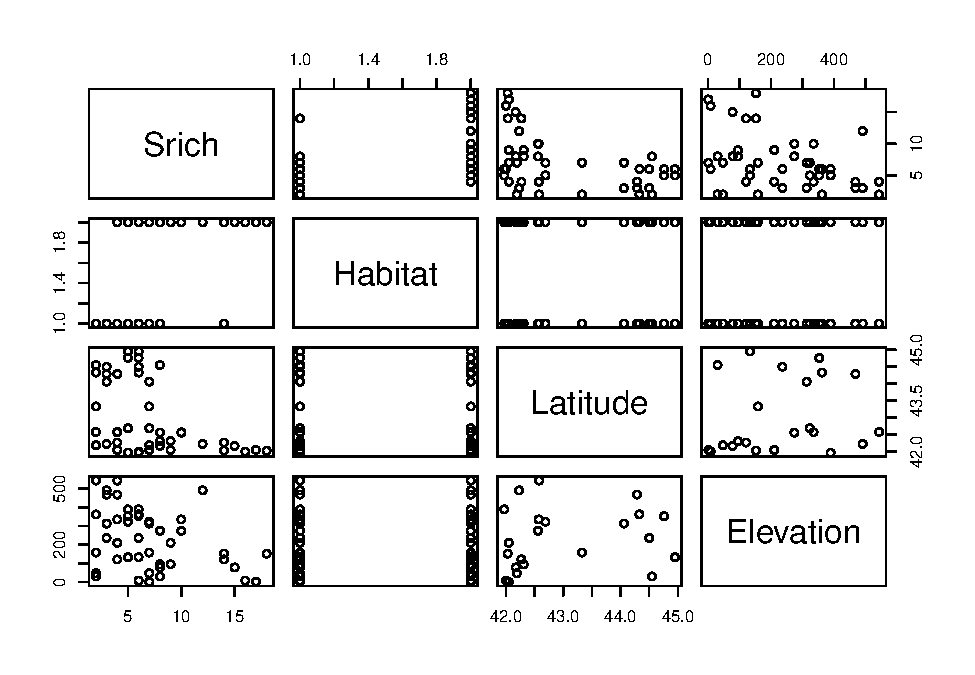
\includegraphics{_main_files/figure-latex/explo2-1.pdf}

\begin{Shaded}
\begin{Highlighting}[]
\KeywordTok{round}\NormalTok{(}\KeywordTok{cor}\NormalTok{(h[, }\KeywordTok{c}\NormalTok{(}\DecValTok{2}\NormalTok{, }\DecValTok{4}\OperatorTok{:}\DecValTok{5}\NormalTok{)]), }\DecValTok{2}\NormalTok{)}
\end{Highlighting}
\end{Shaded}

\begin{verbatim}
##           Srich Latitude Elevation
## Srich      1.00    -0.44     -0.38
## Latitude  -0.44     1.00      0.18
## Elevation -0.38     0.18      1.00
\end{verbatim}

\begin{Shaded}
\begin{Highlighting}[]
\KeywordTok{plot}\NormalTok{(}\KeywordTok{table}\NormalTok{(h}\OperatorTok{$}\NormalTok{Srich), }\DataTypeTok{xlab =} \StringTok{"Número de especies"}\NormalTok{, }\DataTypeTok{ylab =} \StringTok{"Frecuencia"}\NormalTok{)}
\end{Highlighting}
\end{Shaded}

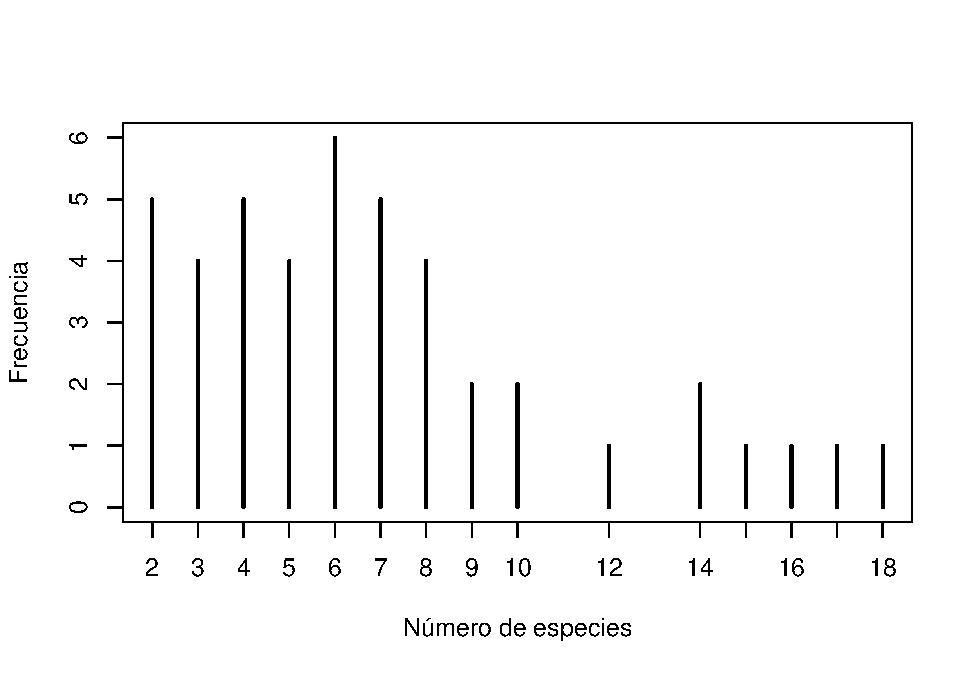
\includegraphics{_main_files/figure-latex/explo2-2.pdf}

\begin{Shaded}
\begin{Highlighting}[]
\KeywordTok{hist}\NormalTok{(h}\OperatorTok{$}\NormalTok{Srich, }\DataTypeTok{xlab =} \StringTok{"Número de especies"}\NormalTok{, }\DataTypeTok{ylab =} \StringTok{"Frecuencia relativa"}\NormalTok{, }\DataTypeTok{main =} \StringTok{""}\NormalTok{, }\DataTypeTok{freq =} \OtherTok{FALSE}\NormalTok{)}

\CommentTok{# Ajuste de distribución a los datos}
\NormalTok{sim.pois <-}\StringTok{ }\KeywordTok{dpois}\NormalTok{(}\DataTypeTok{x =} \DecValTok{0}\OperatorTok{:}\KeywordTok{max}\NormalTok{(h}\OperatorTok{$}\NormalTok{Srich), }\DataTypeTok{lambda =} \KeywordTok{mean}\NormalTok{(h}\OperatorTok{$}\NormalTok{Srich))}
\KeywordTok{lines}\NormalTok{(}\DataTypeTok{x =} \DecValTok{0}\OperatorTok{:}\KeywordTok{max}\NormalTok{(h}\OperatorTok{$}\NormalTok{Srich), }\DataTypeTok{y =}\NormalTok{ sim.pois, }\DataTypeTok{col =} \StringTok{"blue"}\NormalTok{, }\DataTypeTok{lwd =} \DecValTok{2}\NormalTok{, }\DataTypeTok{type =} \StringTok{"b"}\NormalTok{)}
\end{Highlighting}
\end{Shaded}

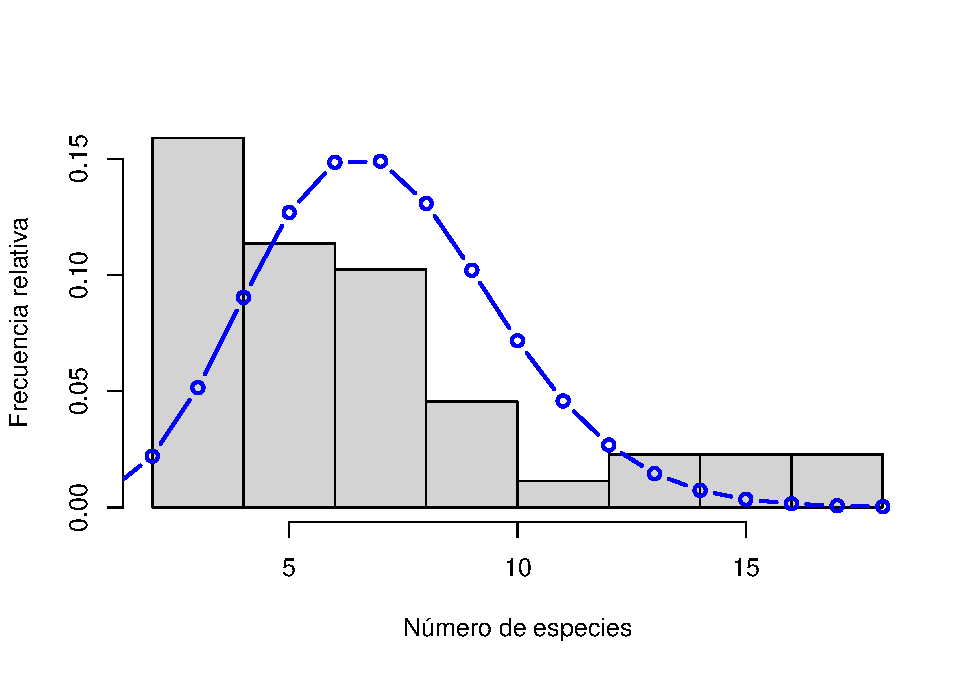
\includegraphics{_main_files/figure-latex/explo2-3.pdf}

\begin{Shaded}
\begin{Highlighting}[]
\KeywordTok{var}\NormalTok{(h}\OperatorTok{$}\NormalTok{Srich)}\OperatorTok{/}\KeywordTok{mean}\NormalTok{(h}\OperatorTok{$}\NormalTok{Srich)}
\end{Highlighting}
\end{Shaded}

\begin{verbatim}
## [1] 2.566343
\end{verbatim}

\hypertarget{glms-poisson-y-quasi-poisson}{%
\subsection{GLMs Poisson y quasi-Poisson}\label{glms-poisson-y-quasi-poisson}}

\hypertarget{glm-poisson}{%
\subsubsection{GLM Poisson}\label{glm-poisson}}

\begin{Shaded}
\begin{Highlighting}[]
\NormalTok{m.pois <-}\StringTok{ }\KeywordTok{glm}\NormalTok{(Srich }\OperatorTok{~}\StringTok{ }\NormalTok{Latitude }\OperatorTok{+}\StringTok{ }\NormalTok{Elevation }\OperatorTok{+}\StringTok{ }\NormalTok{Habitat, }\DataTypeTok{family =}\NormalTok{ poisson, }\DataTypeTok{data =}\NormalTok{ h)}
\KeywordTok{summary}\NormalTok{(m.pois)}
\end{Highlighting}
\end{Shaded}

\begin{verbatim}
## 
## Call:
## glm(formula = Srich ~ Latitude + Elevation + Habitat, family = poisson, 
##     data = h)
## 
## Deviance Residuals: 
##      Min        1Q    Median        3Q       Max  
## -2.20939  -0.72643  -0.05933   0.51571   2.60147  
## 
## Coefficients:
##                 Estimate Std. Error z value Pr(>|z|)    
## (Intercept)   11.9368121  2.6214970   4.553 5.28e-06 ***
## Latitude      -0.2357930  0.0616638  -3.824 0.000131 ***
## Elevation     -0.0011411  0.0003749  -3.044 0.002337 ** 
## HabitatForest  0.6354389  0.1195664   5.315 1.07e-07 ***
## ---
## Signif. codes:  0 '***' 0.001 '**' 0.01 '*' 0.05 '.' 0.1 ' ' 1
## 
## (Dispersion parameter for poisson family taken to be 1)
## 
##     Null deviance: 102.76  on 43  degrees of freedom
## Residual deviance:  40.69  on 40  degrees of freedom
## AIC: 209.04
## 
## Number of Fisher Scoring iterations: 4
\end{verbatim}

\hypertarget{glm-quasi-poisson}{%
\subsubsection{GLM quasi-Poisson}\label{glm-quasi-poisson}}

\begin{Shaded}
\begin{Highlighting}[]
\NormalTok{m.qpois <-}\StringTok{ }\KeywordTok{glm}\NormalTok{(Srich }\OperatorTok{~}\StringTok{ }\NormalTok{Latitude }\OperatorTok{+}\StringTok{ }\NormalTok{Elevation }\OperatorTok{+}\StringTok{ }\NormalTok{Habitat, }\DataTypeTok{family =}\NormalTok{ quasipoisson, }\DataTypeTok{data =}\NormalTok{ h)}
\KeywordTok{summary}\NormalTok{(m.qpois)}
\end{Highlighting}
\end{Shaded}

\begin{verbatim}
## 
## Call:
## glm(formula = Srich ~ Latitude + Elevation + Habitat, family = quasipoisson, 
##     data = h)
## 
## Deviance Residuals: 
##      Min        1Q    Median        3Q       Max  
## -2.20939  -0.72643  -0.05933   0.51571   2.60147  
## 
## Coefficients:
##                 Estimate Std. Error t value Pr(>|t|)    
## (Intercept)   11.9368121  2.6594025   4.489 5.94e-05 ***
## Latitude      -0.2357930  0.0625554  -3.769 0.000529 ***
## Elevation     -0.0011411  0.0003803  -3.000 0.004626 ** 
## HabitatForest  0.6354389  0.1212952   5.239 5.52e-06 ***
## ---
## Signif. codes:  0 '***' 0.001 '**' 0.01 '*' 0.05 '.' 0.1 ' ' 1
## 
## (Dispersion parameter for quasipoisson family taken to be 1.029128)
## 
##     Null deviance: 102.76  on 43  degrees of freedom
## Residual deviance:  40.69  on 40  degrees of freedom
## AIC: NA
## 
## Number of Fisher Scoring iterations: 4
\end{verbatim}

\begin{Shaded}
\begin{Highlighting}[]
\CommentTok{# Parámetro de sobredispersión}
\NormalTok{resid <-}\StringTok{ }\KeywordTok{residuals}\NormalTok{(m.qpois, }\DataTypeTok{type =} \StringTok{"pearson"}\NormalTok{)}
\NormalTok{nparam <-}\StringTok{ }\KeywordTok{length}\NormalTok{(m.qpois}\OperatorTok{$}\NormalTok{coeff)}
\NormalTok{ndatos <-}\StringTok{ }\KeywordTok{nrow}\NormalTok{(h)}
\NormalTok{disp.param <-}\StringTok{ }\KeywordTok{sum}\NormalTok{(resid}\OperatorTok{^}\DecValTok{2}\NormalTok{)}\OperatorTok{/}\NormalTok{(ndatos }\OperatorTok{-}\StringTok{ }\NormalTok{nparam)}
\NormalTok{disp.param}
\end{Highlighting}
\end{Shaded}

\begin{verbatim}
## [1] 1.029116
\end{verbatim}

\begin{Shaded}
\begin{Highlighting}[]
\NormalTok{m.qpois.null <-}\StringTok{ }\KeywordTok{glm}\NormalTok{(Srich }\OperatorTok{~}\StringTok{ }\DecValTok{1}\NormalTok{, }\DataTypeTok{family =}\NormalTok{ quasipoisson, }\DataTypeTok{data =}\NormalTok{ h)}
\KeywordTok{summary}\NormalTok{(m.qpois.null)}
\end{Highlighting}
\end{Shaded}

\begin{verbatim}
## 
## Call:
## glm(formula = Srich ~ 1, family = quasipoisson, data = h)
## 
## Deviance Residuals: 
##     Min       1Q   Median       3Q      Max  
## -2.2409  -1.2420  -0.3959   0.4492   3.4539  
## 
## Coefficients:
##             Estimate Std. Error t value Pr(>|t|)    
## (Intercept)  1.94915    0.09113   21.39   <2e-16 ***
## ---
## Signif. codes:  0 '***' 0.001 '**' 0.01 '*' 0.05 '.' 0.1 ' ' 1
## 
## (Dispersion parameter for quasipoisson family taken to be 2.566343)
## 
##     Null deviance: 102.76  on 43  degrees of freedom
## Residual deviance: 102.76  on 43  degrees of freedom
## AIC: NA
## 
## Number of Fisher Scoring iterations: 5
\end{verbatim}

\begin{Shaded}
\begin{Highlighting}[]
\KeywordTok{library}\NormalTok{(DHARMa)}
\KeywordTok{testDispersion}\NormalTok{(m.pois)}
\end{Highlighting}
\end{Shaded}

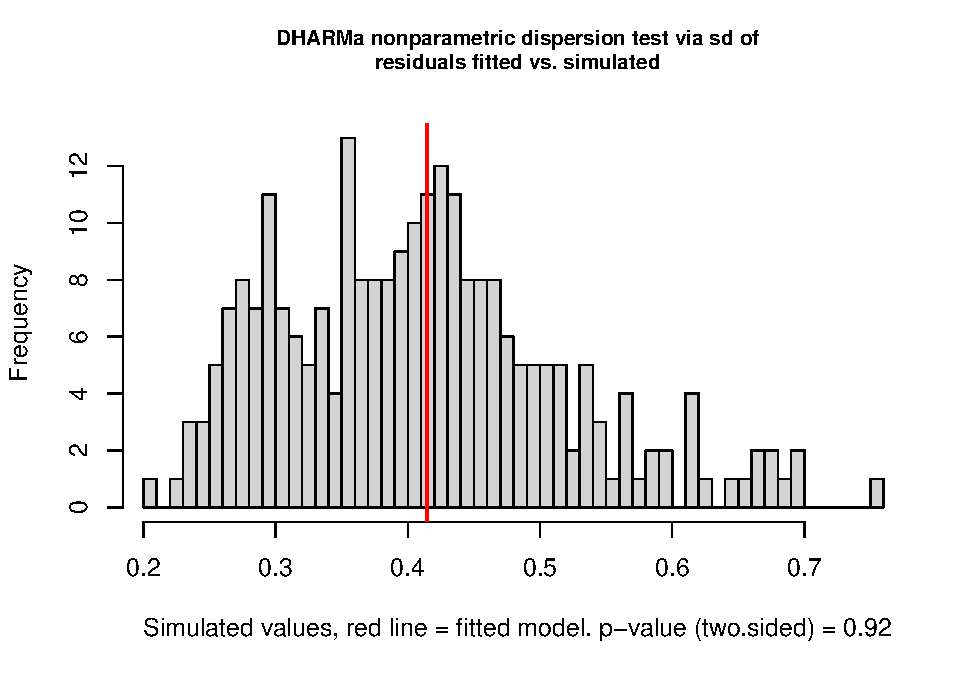
\includegraphics{_main_files/figure-latex/glm quasipoisson-1.pdf}

\begin{verbatim}
## 
##  DHARMa nonparametric dispersion test via sd of residuals fitted vs. simulated
## 
## data:  simulationOutput
## dispersion = 1.0136, p-value = 0.92
## alternative hypothesis: two.sided
\end{verbatim}

\hypertarget{diagnuxf3sticos-1}{%
\subsubsection{Diagnósticos}\label{diagnuxf3sticos-1}}

\begin{Shaded}
\begin{Highlighting}[]
\NormalTok{residP <-}\StringTok{ }\KeywordTok{resid}\NormalTok{(m.qpois, }\DataTypeTok{type =} \StringTok{"pearson"}\NormalTok{)  }\CommentTok{# residuos de Pearson }
\NormalTok{residD <-}\StringTok{ }\KeywordTok{resid}\NormalTok{(m.qpois, }\DataTypeTok{type =} \StringTok{"deviance"}\NormalTok{) }\CommentTok{# residuos de devianza }
\NormalTok{pred <-}\StringTok{ }\KeywordTok{predict}\NormalTok{(m.qpois, }\DataTypeTok{type =} \StringTok{"response"}\NormalTok{) }\CommentTok{# valores predichos }
\KeywordTok{plot}\NormalTok{(pred, residP) }
\end{Highlighting}
\end{Shaded}

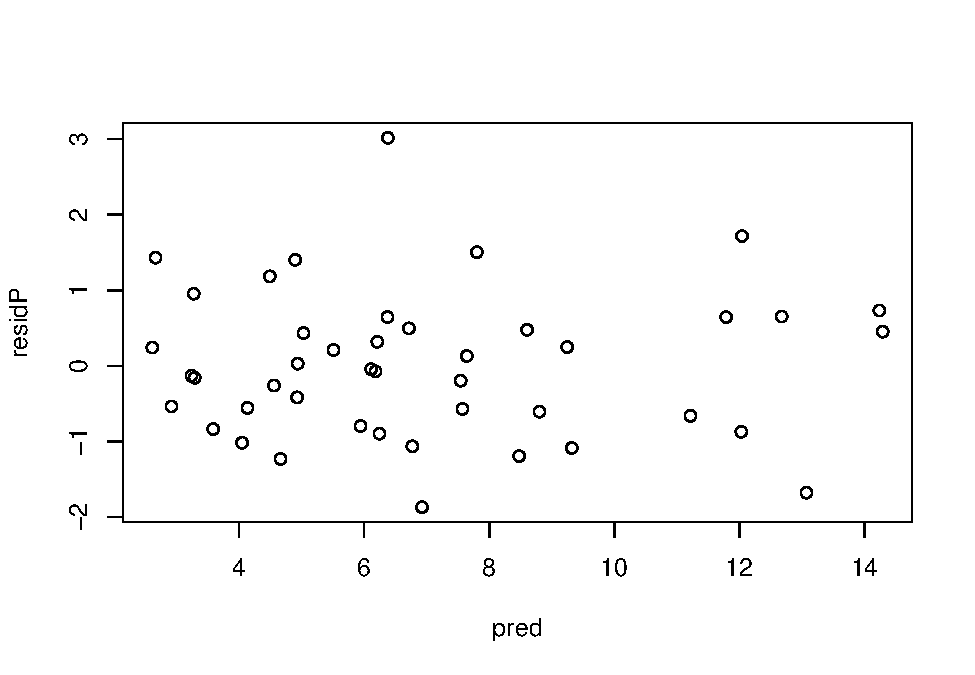
\includegraphics{_main_files/figure-latex/validacion glm poisson-1.pdf}

\begin{Shaded}
\begin{Highlighting}[]
\KeywordTok{plot}\NormalTok{(pred, residD)}
\end{Highlighting}
\end{Shaded}

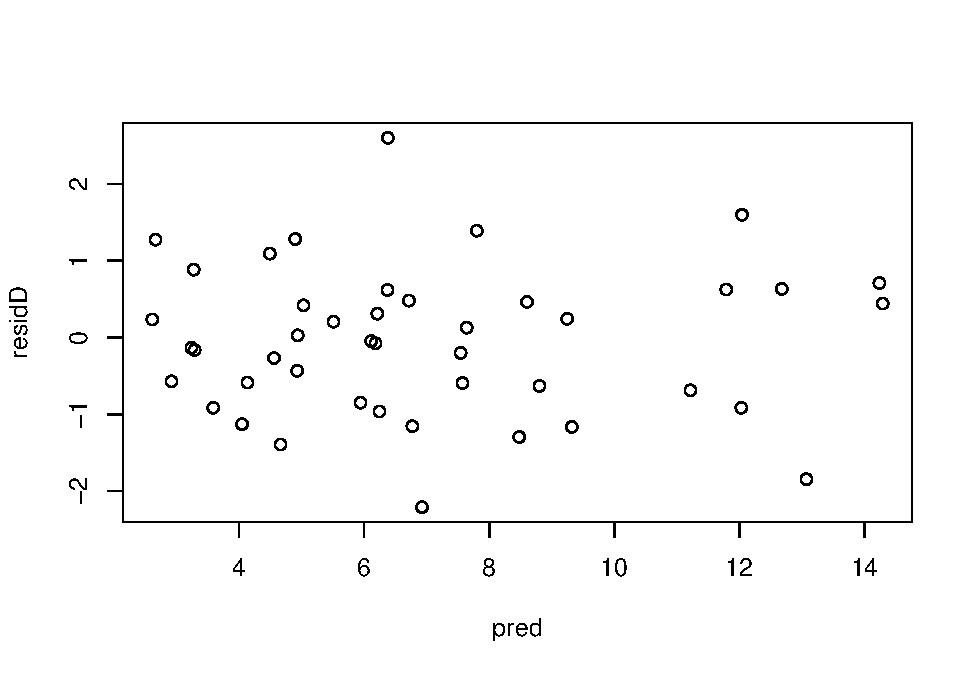
\includegraphics{_main_files/figure-latex/validacion glm poisson-2.pdf}

\begin{Shaded}
\begin{Highlighting}[]
\KeywordTok{plot}\NormalTok{(}\KeywordTok{simulateResiduals}\NormalTok{(}\DataTypeTok{fittedModel =}\NormalTok{ m.pois))}
\end{Highlighting}
\end{Shaded}

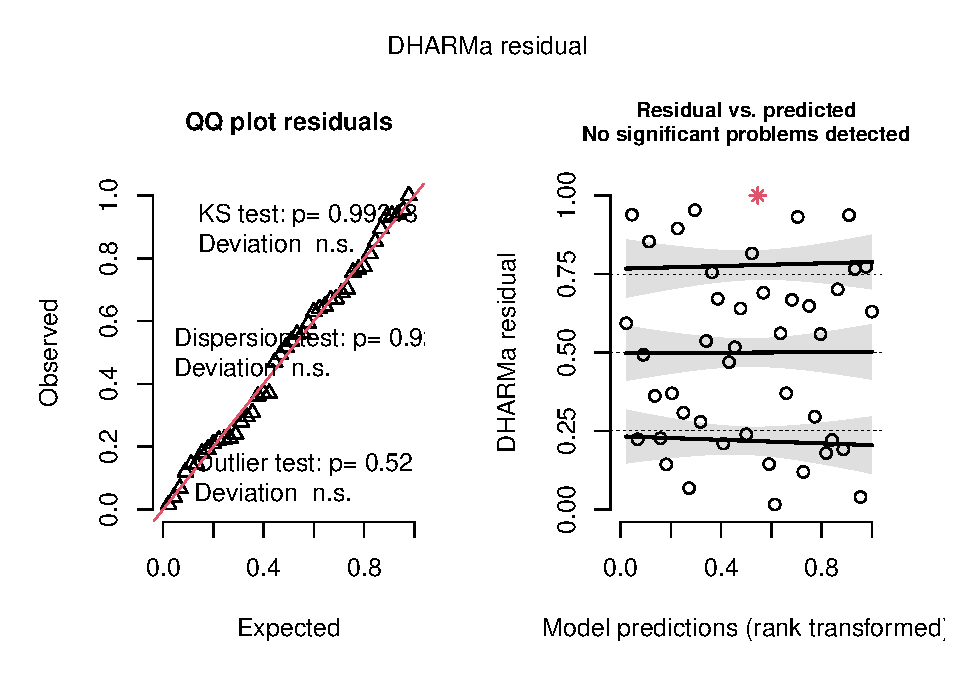
\includegraphics{_main_files/figure-latex/validacion glm poisson-3.pdf}

\hypertarget{bondad-del-ajuste-1}{%
\subsubsection{Bondad del ajuste}\label{bondad-del-ajuste-1}}

\begin{Shaded}
\begin{Highlighting}[]
\DecValTok{1} \OperatorTok{-}\StringTok{ }\NormalTok{(m.qpois}\OperatorTok{$}\NormalTok{dev}\OperatorTok{/}\NormalTok{m.qpois}\OperatorTok{$}\NormalTok{null) }\CommentTok{# Pseudo-R2}
\end{Highlighting}
\end{Shaded}

\begin{verbatim}
## [1] 0.6040372
\end{verbatim}

\hypertarget{ecuaciuxf3n-1}{%
\subsubsection{Ecuación}\label{ecuaciuxf3n-1}}

\begin{Shaded}
\begin{Highlighting}[]
\KeywordTok{library}\NormalTok{(equatiomatic)}
\KeywordTok{extract_eq}\NormalTok{(m.qpois, }\DataTypeTok{use_coefs =} \OtherTok{TRUE}\NormalTok{, }\DataTypeTok{fix_signs =} \OtherTok{TRUE}\NormalTok{)}
\end{Highlighting}
\end{Shaded}

\begin{equation}
\log ({ \widehat{E( \operatorname{Srich} )} })  = 11.94 - 0.24(\operatorname{Latitude}) + 0(\operatorname{Elevation}) + 0.64(\operatorname{Habitat}_{\operatorname{Forest}})
\end{equation}

\hypertarget{gruxe1fico-del-modelo-1}{%
\subsubsection{Gráfico del modelo}\label{gruxe1fico-del-modelo-1}}

\begin{Shaded}
\begin{Highlighting}[]
\KeywordTok{library}\NormalTok{(visreg)}
\KeywordTok{visreg}\NormalTok{(}\DataTypeTok{fit =}\NormalTok{ m.qpois, }\DataTypeTok{xvar =} \StringTok{"Latitude"}\NormalTok{, }\DataTypeTok{by =} \StringTok{"Habitat"}\NormalTok{, }\DataTypeTok{overlay =} \OtherTok{TRUE}\NormalTok{, }
       \DataTypeTok{scale =} \StringTok{"response"}\NormalTok{, }\DataTypeTok{xlab =} \StringTok{"Latitud"}\NormalTok{, }\DataTypeTok{ylab =} \StringTok{"Número de especies"}\NormalTok{,}
       \DataTypeTok{type =} \StringTok{"conditional"}\NormalTok{, }\DataTypeTok{cond =} \KeywordTok{list}\NormalTok{(}\DataTypeTok{Latitude =} \KeywordTok{mean}\NormalTok{(h}\OperatorTok{$}\NormalTok{Latitude), }\DataTypeTok{Elevation =} \KeywordTok{mean}\NormalTok{(h}\OperatorTok{$}\NormalTok{Elevation))) }
\NormalTok{bg <-}\StringTok{ }\NormalTok{h[h}\OperatorTok{$}\NormalTok{Habitat }\OperatorTok{==}\StringTok{ "Bog"}\NormalTok{, ] }
\NormalTok{ft <-}\StringTok{ }\NormalTok{h[h}\OperatorTok{$}\NormalTok{Habitat }\OperatorTok{==}\StringTok{ "Forest"}\NormalTok{, ] }
\KeywordTok{points}\NormalTok{(bg}\OperatorTok{$}\NormalTok{Latitude, bg}\OperatorTok{$}\NormalTok{Srich, }\DataTypeTok{pch=}\DecValTok{19}\NormalTok{, }\DataTypeTok{col =} \StringTok{"red"}\NormalTok{) }
\KeywordTok{points}\NormalTok{(ft}\OperatorTok{$}\NormalTok{Latitude, ft}\OperatorTok{$}\NormalTok{Srich, }\DataTypeTok{pch=}\DecValTok{19}\NormalTok{, }\DataTypeTok{col =} \StringTok{"blue"}\NormalTok{)}
\end{Highlighting}
\end{Shaded}

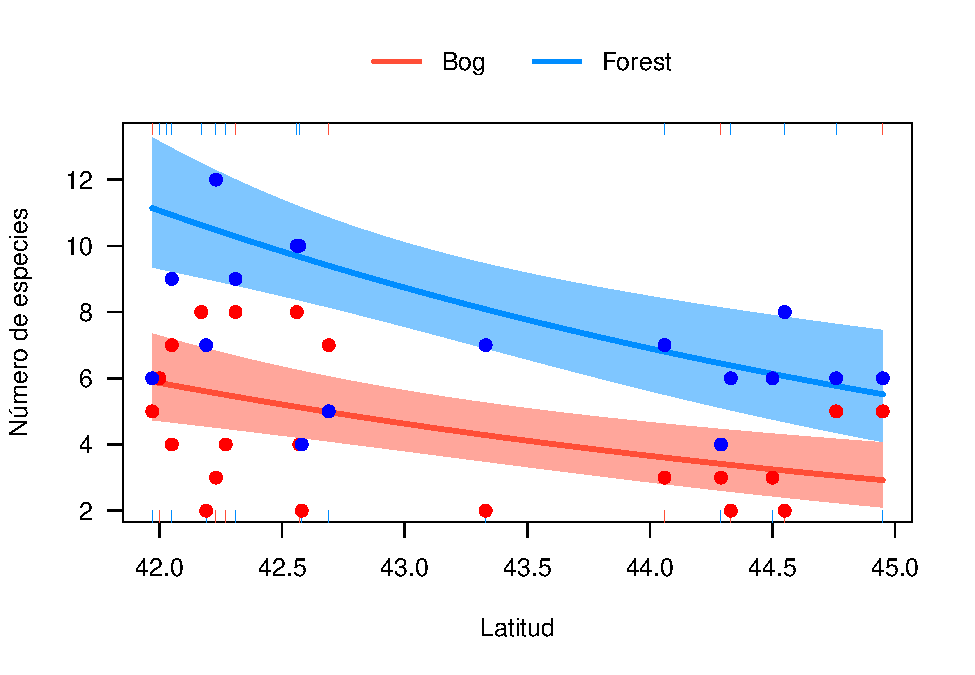
\includegraphics{_main_files/figure-latex/grafico glm poisson-1.pdf}

\hypertarget{glm-binomial-negativo}{%
\subsection{GLM binomial negativo}\label{glm-binomial-negativo}}

Leong et al.~(2014) estudiaron el efecto del paisaje (urbano, agrícola y natural) sobre el número de interacciones de polinizadores nativos en \(Centaurea solstitialis\) (Asteraceae). Se quiere evaluar si existen diferencias en el número de interacciones (\texttt{total}) entre los 3 tipos de ambientes (\texttt{type}) teniendo en cuenta la temperatura (\texttt{temp}) y la velocidad del viento (\texttt{wind}).

\begin{Shaded}
\begin{Highlighting}[]
\CommentTok{# Análisis exploratorio}
\NormalTok{pol <-}\StringTok{ }\KeywordTok{read.table}\NormalTok{(}\StringTok{"bees_data.txt"}\NormalTok{, }\DataTypeTok{header =}\NormalTok{ T) }
\KeywordTok{str}\NormalTok{(pol)}
\end{Highlighting}
\end{Shaded}

\begin{verbatim}
## 'data.frame':    36 obs. of  34 variables:
##  $ locality    : chr  "arabian" "arabian" "arabian" "bdm_f" ...
##  $ type        : chr  "a" "a" "a" "n" ...
##  $ lat         : num  37.9 37.9 37.9 38 38 ...
##  $ long        : num  -122 -122 -122 -122 -122 ...
##  $ water       : int  0 0 0 0 0 0 0 0 0 0 ...
##  $ urban       : int  18900 18900 18900 37800 37800 37800 4500 4500 4500 198000 ...
##  $ agr         : int  252000 252000 252000 0 0 0 16200 16200 16200 558000 ...
##  $ natural     : int  513900 513900 513900 747900 747900 747900 765000 765000 765000 32400 ...
##  $ bare        : int  1800 1800 1800 0 0 0 0 0 0 0 ...
##  $ bloom.cat   : int  3 3 3 3 3 3 4 4 4 4 ...
##  $ time        : chr  "am" "mid" "pm" "am" ...
##  $ wind        : num  2.7 1.35 0.8 2.3 3.75 3.7 2.4 2.15 2.5 0.85 ...
##  $ temp        : num  80.9 94.3 91.1 86.1 87.4 ...
##  $ hb          : int  70 44 24 34 24 27 40 29 14 88 ...
##  $ bumble      : int  0 0 0 1 0 4 0 0 0 0 ...
##  $ carpenter   : int  0 0 0 0 0 1 0 0 0 0 ...
##  $ hlb         : int  2 0 0 7 2 0 9 2 0 1 ...
##  $ svastra     : int  0 0 0 0 0 0 0 0 0 0 ...
##  $ agtex       : int  4 1 0 0 0 0 0 0 0 0 ...
##  $ ssb.med     : int  0 0 0 0 0 0 1 0 0 1 ...
##  $ ssb.small   : int  0 0 1 4 0 4 1 3 2 9 ...
##  $ sdb.round   : int  1 0 6 1 1 1 2 3 4 2 ...
##  $ sdb.shield  : int  3 2 2 0 2 0 0 0 0 0 ...
##  $ shbb.large  : int  0 0 0 0 0 0 0 0 0 2 ...
##  $ shbb.med    : int  0 1 0 4 0 0 8 5 5 2 ...
##  $ shbb.small  : int  1 3 0 0 0 0 1 1 1 0 ...
##  $ anthidium   : int  0 0 0 0 0 0 0 0 0 0 ...
##  $ cuckoo      : int  0 0 0 0 0 0 1 0 0 0 ...
##  $ total.native: int  11 7 9 17 5 10 23 14 12 17 ...
##  $ total       : int  81 51 33 51 29 37 63 43 26 105 ...
##  $ min         : int  90 90 90 90 90 90 90 90 90 90 ...
##  $ num.group   : int  6 5 4 6 4 5 8 6 5 7 ...
##  $ shannon     : num  0.597 0.575 0.817 1.096 0.642 ...
##  $ even        : num  0.333 0.357 0.59 0.612 0.463 ...
\end{verbatim}

\begin{Shaded}
\begin{Highlighting}[]
\NormalTok{pol}\OperatorTok{$}\NormalTok{habitat <-}\StringTok{ }\KeywordTok{factor}\NormalTok{(pol}\OperatorTok{$}\NormalTok{type, }\DataTypeTok{levels =} \KeywordTok{c}\NormalTok{(}\StringTok{"n"}\NormalTok{, }\StringTok{"a"}\NormalTok{, }\StringTok{"u"}\NormalTok{))}
\KeywordTok{pairs}\NormalTok{(pol[, }\KeywordTok{c}\NormalTok{(}\StringTok{"habitat"}\NormalTok{, }\StringTok{"temp"}\NormalTok{, }\StringTok{"wind"}\NormalTok{, }\StringTok{"total"}\NormalTok{)])}
\end{Highlighting}
\end{Shaded}

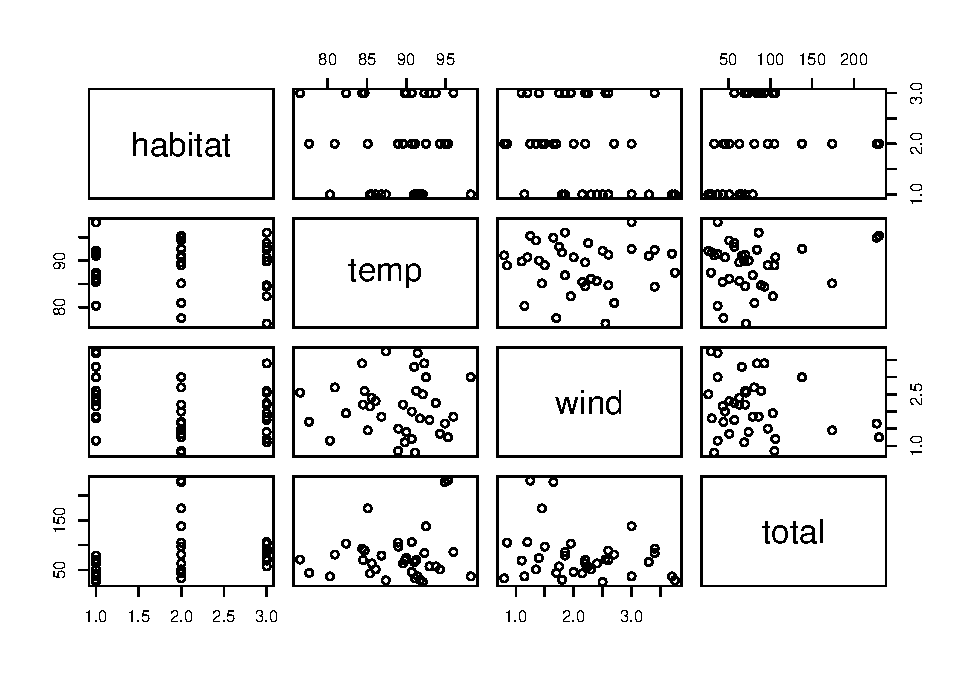
\includegraphics{_main_files/figure-latex/explo3-1.pdf}

\begin{Shaded}
\begin{Highlighting}[]
\KeywordTok{boxplot}\NormalTok{(pol}\OperatorTok{$}\NormalTok{total }\OperatorTok{~}\StringTok{ }\NormalTok{pol}\OperatorTok{$}\NormalTok{habitat)}
\end{Highlighting}
\end{Shaded}

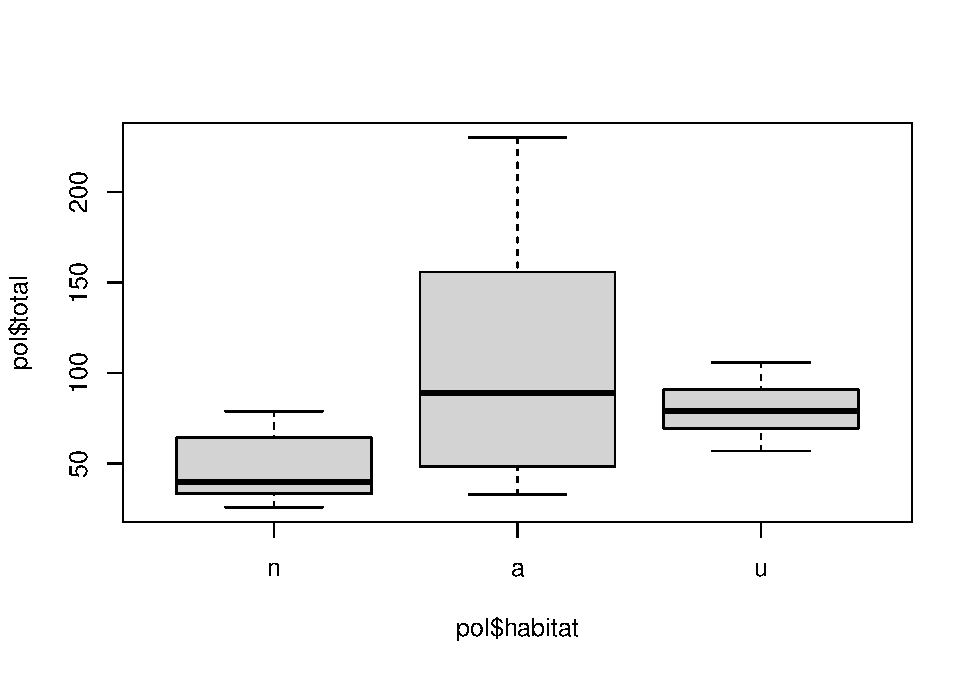
\includegraphics{_main_files/figure-latex/explo3-2.pdf}

\begin{Shaded}
\begin{Highlighting}[]
\KeywordTok{cor}\NormalTok{(pol}\OperatorTok{$}\NormalTok{temp, pol}\OperatorTok{$}\NormalTok{wind)}
\end{Highlighting}
\end{Shaded}

\begin{verbatim}
## [1] -0.02087349
\end{verbatim}

\begin{Shaded}
\begin{Highlighting}[]
\KeywordTok{hist}\NormalTok{(pol}\OperatorTok{$}\NormalTok{total, }\DataTypeTok{xlab =} \StringTok{"Número de interacciones"}\NormalTok{, }\DataTypeTok{ylab =} \StringTok{"Frecuencia relativa"}\NormalTok{, }\DataTypeTok{main =} \StringTok{""}\NormalTok{, }\DataTypeTok{freq =} \OtherTok{FALSE}\NormalTok{, }\DataTypeTok{ylim =} \KeywordTok{c}\NormalTok{(}\DecValTok{0}\NormalTok{, }\FloatTok{0.05}\NormalTok{))}

\CommentTok{# Ajuste de distribución a los datos}
\NormalTok{sim.pois <-}\StringTok{ }\KeywordTok{dpois}\NormalTok{(}\DataTypeTok{x =} \DecValTok{0}\OperatorTok{:}\KeywordTok{max}\NormalTok{(pol}\OperatorTok{$}\NormalTok{total), }\DataTypeTok{lambda =} \KeywordTok{mean}\NormalTok{(pol}\OperatorTok{$}\NormalTok{total))}
\KeywordTok{lines}\NormalTok{(}\DataTypeTok{x =} \DecValTok{0}\OperatorTok{:}\KeywordTok{max}\NormalTok{(pol}\OperatorTok{$}\NormalTok{total), }\DataTypeTok{y =}\NormalTok{ sim.pois, }\DataTypeTok{col =} \StringTok{"blue"}\NormalTok{, }\DataTypeTok{lwd =} \DecValTok{2}\NormalTok{, }\DataTypeTok{type =} \StringTok{"b"}\NormalTok{)}
\end{Highlighting}
\end{Shaded}

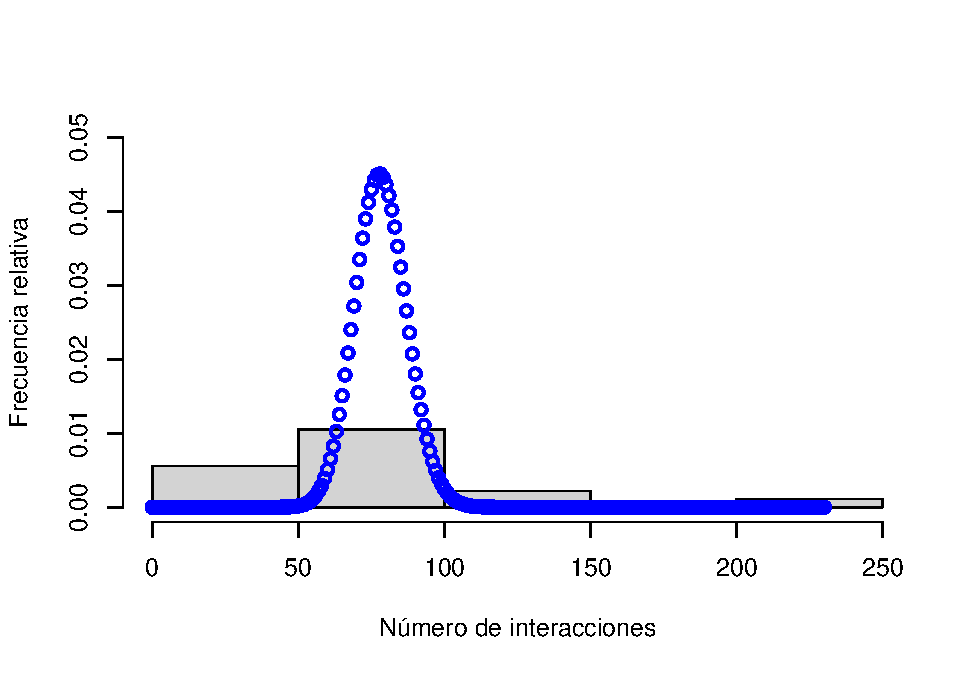
\includegraphics{_main_files/figure-latex/explo3-3.pdf}

\begin{Shaded}
\begin{Highlighting}[]
\KeywordTok{var}\NormalTok{(pol}\OperatorTok{$}\NormalTok{total)}\OperatorTok{/}\KeywordTok{mean}\NormalTok{(pol}\OperatorTok{$}\NormalTok{total)}
\end{Highlighting}
\end{Shaded}

\begin{verbatim}
## [1] 30.01128
\end{verbatim}

\hypertarget{chequear-sobredispersiuxf3n}{%
\subsubsection{Chequear sobredispersión}\label{chequear-sobredispersiuxf3n}}

\begin{Shaded}
\begin{Highlighting}[]
\NormalTok{mqpoi.pol <-}\StringTok{ }\KeywordTok{glm}\NormalTok{(total }\OperatorTok{~}\StringTok{ }\NormalTok{habitat }\OperatorTok{+}\StringTok{ }\NormalTok{temp }\OperatorTok{+}\StringTok{ }\NormalTok{wind, }\DataTypeTok{family =}\NormalTok{ quasipoisson, }\DataTypeTok{data =}\NormalTok{ pol) }
\KeywordTok{summary}\NormalTok{(mqpoi.pol)}
\end{Highlighting}
\end{Shaded}

\begin{verbatim}
## 
## Call:
## glm(formula = total ~ habitat + temp + wind, family = quasipoisson, 
##     data = pol)
## 
## Deviance Residuals: 
##     Min       1Q   Median       3Q      Max  
## -8.7048  -2.7630  -0.5307   2.2527   8.9461  
## 
## Coefficients:
##              Estimate Std. Error t value Pr(>|t|)   
## (Intercept)  2.244844   1.518268   1.479  0.14935   
## habitata     0.813256   0.238963   3.403  0.00186 **
## habitatu     0.535908   0.233539   2.295  0.02868 * 
## temp         0.018127   0.016226   1.117  0.27252   
## wind        -0.001247   0.116820  -0.011  0.99155   
## ---
## Signif. codes:  0 '***' 0.001 '**' 0.01 '*' 0.05 '.' 0.1 ' ' 1
## 
## (Dispersion parameter for quasipoisson family taken to be 18.37662)
## 
##     Null deviance: 876.87  on 35  degrees of freedom
## Residual deviance: 565.09  on 31  degrees of freedom
## AIC: NA
## 
## Number of Fisher Scoring iterations: 5
\end{verbatim}

\begin{Shaded}
\begin{Highlighting}[]
\KeywordTok{library}\NormalTok{(DHARMa)}
\NormalTok{mpoi.pol <-}\StringTok{ }\KeywordTok{glm}\NormalTok{(total }\OperatorTok{~}\StringTok{ }\NormalTok{habitat }\OperatorTok{+}\StringTok{ }\NormalTok{temp }\OperatorTok{+}\StringTok{ }\NormalTok{wind, }\DataTypeTok{family =}\NormalTok{ poisson, }\DataTypeTok{data =}\NormalTok{ pol)}
\KeywordTok{testDispersion}\NormalTok{(mpoi.pol)}
\end{Highlighting}
\end{Shaded}

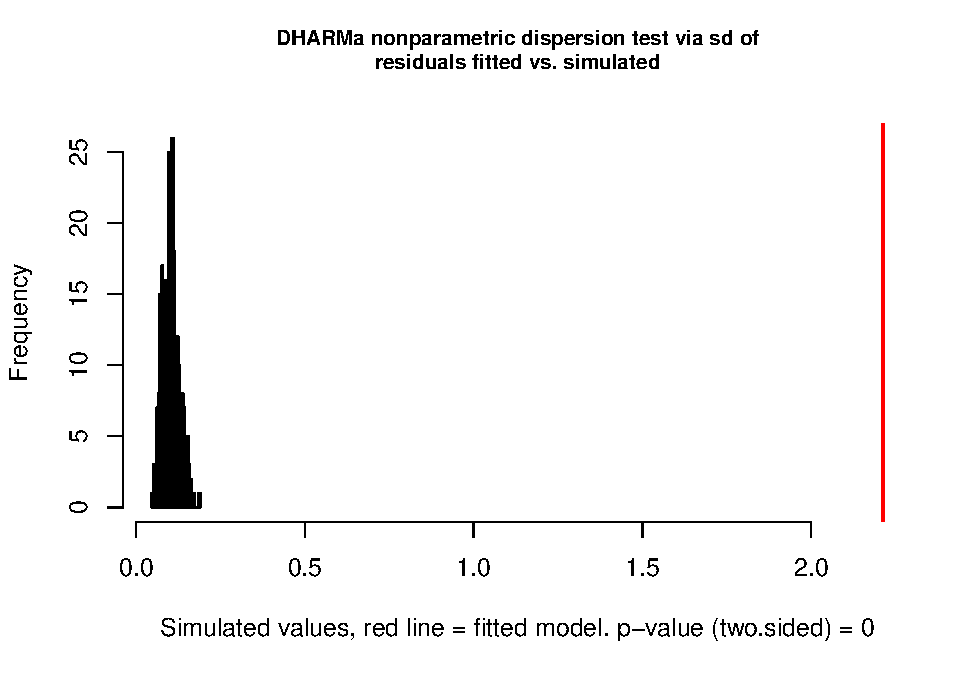
\includegraphics{_main_files/figure-latex/sobredispersion-1.pdf}

\begin{verbatim}
## 
##  DHARMa nonparametric dispersion test via sd of residuals fitted vs. simulated
## 
## data:  simulationOutput
## dispersion = 21.413, p-value < 2.2e-16
## alternative hypothesis: two.sided
\end{verbatim}

\hypertarget{validaciuxf3n-del-modelo-quasi-poisson}{%
\subsubsection{Validación del modelo quasi-Poisson}\label{validaciuxf3n-del-modelo-quasi-poisson}}

\begin{Shaded}
\begin{Highlighting}[]
\KeywordTok{plot}\NormalTok{(}\KeywordTok{simulateResiduals}\NormalTok{(}\DataTypeTok{fittedModel =}\NormalTok{ mpoi.pol))}
\end{Highlighting}
\end{Shaded}

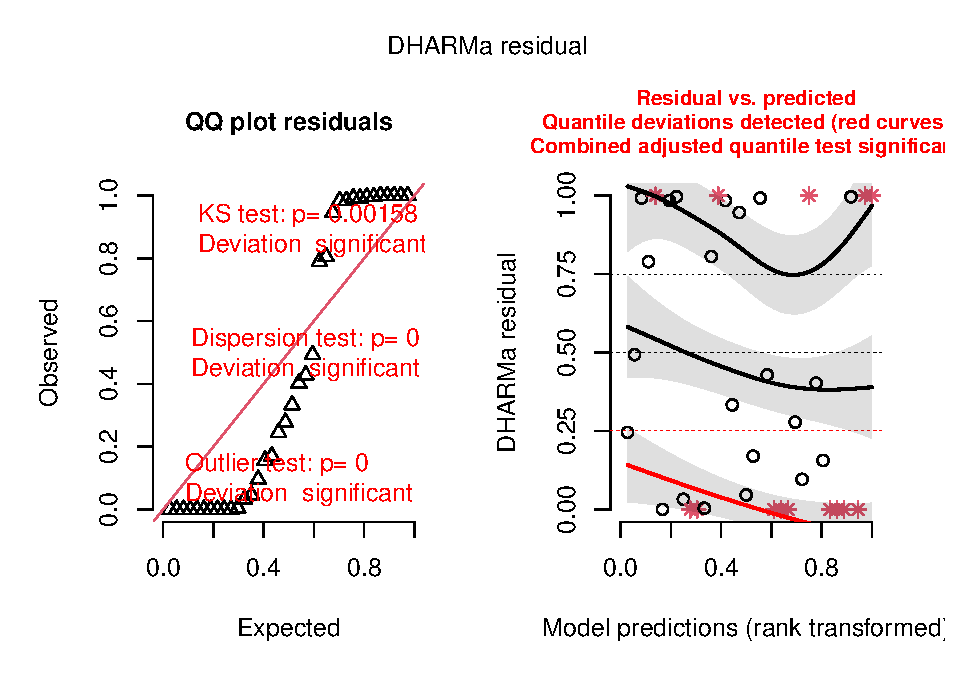
\includegraphics{_main_files/figure-latex/validacion glm quasipoisson-1.pdf}

\hypertarget{modelo-binomial-negativo}{%
\subsubsection{Modelo binomial negativo}\label{modelo-binomial-negativo}}

\begin{Shaded}
\begin{Highlighting}[]
\KeywordTok{library}\NormalTok{(MASS)}
\NormalTok{mbn.pol <-}\StringTok{ }\KeywordTok{glm.nb}\NormalTok{(total }\OperatorTok{~}\StringTok{ }\NormalTok{habitat }\OperatorTok{+}\StringTok{ }\NormalTok{temp }\OperatorTok{+}\StringTok{ }\NormalTok{wind, }\DataTypeTok{data =}\NormalTok{ pol) }
\KeywordTok{summary}\NormalTok{(mbn.pol)}
\end{Highlighting}
\end{Shaded}

\begin{verbatim}
## 
## Call:
## glm.nb(formula = total ~ habitat + temp + wind, data = pol, init.theta = 5.957692263, 
##     link = log)
## 
## Deviance Residuals: 
##     Min       1Q   Median       3Q      Max  
## -2.3561  -0.8982  -0.1773   0.5760   1.8680  
## 
## Coefficients:
##             Estimate Std. Error z value Pr(>|z|)    
## (Intercept)  2.82455    1.28889   2.191  0.02842 *  
## habitata     0.78487    0.19397   4.046  5.2e-05 ***
## habitatu     0.52773    0.18051   2.924  0.00346 ** 
## temp         0.01218    0.01406   0.866  0.38652    
## wind        -0.01878    0.10041  -0.187  0.85161    
## ---
## Signif. codes:  0 '***' 0.001 '**' 0.01 '*' 0.05 '.' 0.1 ' ' 1
## 
## (Dispersion parameter for Negative Binomial(5.9577) family taken to be 1)
## 
##     Null deviance: 58.860  on 35  degrees of freedom
## Residual deviance: 36.513  on 31  degrees of freedom
## AIC: 358.06
## 
## Number of Fisher Scoring iterations: 1
## 
## 
##               Theta:  5.96 
##           Std. Err.:  1.47 
## 
##  2 x log-likelihood:  -346.062
\end{verbatim}

\hypertarget{validaciuxf3n-del-modelo-binomial-negativo}{%
\subsubsection{Validación del modelo binomial negativo}\label{validaciuxf3n-del-modelo-binomial-negativo}}

\begin{Shaded}
\begin{Highlighting}[]
\KeywordTok{plot}\NormalTok{(}\KeywordTok{simulateResiduals}\NormalTok{(}\DataTypeTok{fittedModel =}\NormalTok{ mbn.pol))}
\end{Highlighting}
\end{Shaded}

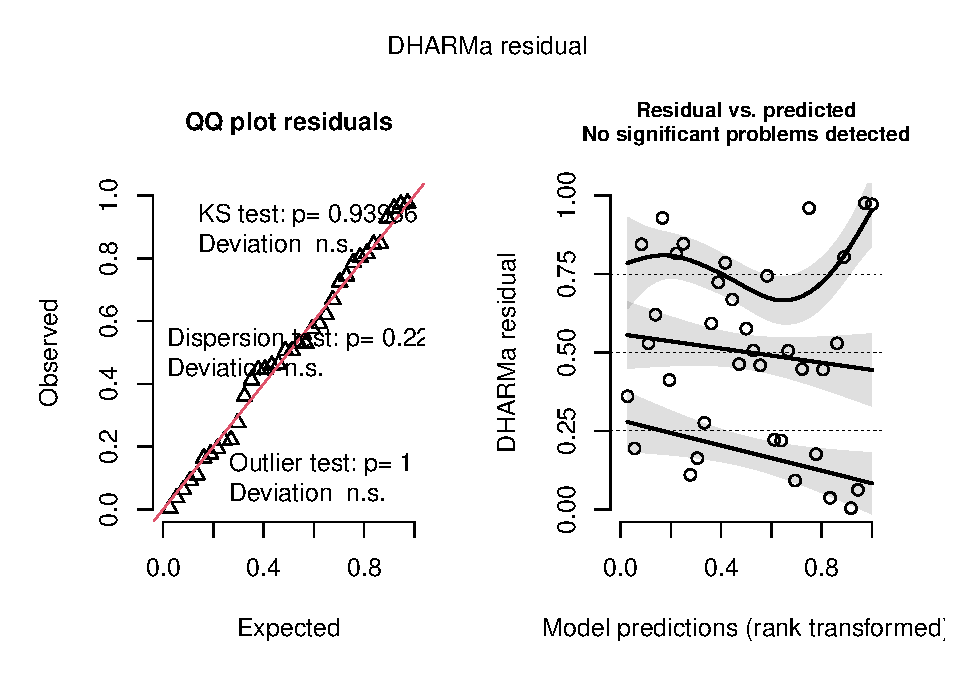
\includegraphics{_main_files/figure-latex/validacion glm BN-1.pdf}

\hypertarget{bondad-del-ajuste-2}{%
\subsubsection{Bondad del ajuste}\label{bondad-del-ajuste-2}}

\begin{Shaded}
\begin{Highlighting}[]
\DecValTok{1} \OperatorTok{-}\StringTok{ }\NormalTok{(mbn.pol}\OperatorTok{$}\NormalTok{dev}\OperatorTok{/}\NormalTok{mbn.pol}\OperatorTok{$}\NormalTok{null) }\CommentTok{# Pseudo-R2}
\end{Highlighting}
\end{Shaded}

\begin{verbatim}
## [1] 0.3796712
\end{verbatim}

\hypertarget{ecuaciuxf3n-2}{%
\subsubsection{Ecuación}\label{ecuaciuxf3n-2}}

\begin{Shaded}
\begin{Highlighting}[]
\KeywordTok{extract_eq}\NormalTok{(mbn.pol, }\DataTypeTok{use_coefs =} \OtherTok{TRUE}\NormalTok{, }\DataTypeTok{fix_signs =} \OtherTok{TRUE}\NormalTok{)}
\end{Highlighting}
\end{Shaded}

\begin{equation}
\log ({ \widehat{E( \operatorname{total} )} })  = 2.82 + 0.78(\operatorname{habitat}_{\operatorname{a}}) + 0.53(\operatorname{habitat}_{\operatorname{u}}) + 0.01(\operatorname{temp}) - 0.02(\operatorname{wind})
\end{equation}

\hypertarget{comparaciones-muxfaltiples}{%
\subsubsection{Comparaciones múltiples}\label{comparaciones-muxfaltiples}}

\begin{Shaded}
\begin{Highlighting}[]
\KeywordTok{library}\NormalTok{(multcomp) }
\end{Highlighting}
\end{Shaded}

\begin{verbatim}
## Loading required package: mvtnorm
\end{verbatim}

\begin{verbatim}
## Loading required package: TH.data
\end{verbatim}

\begin{verbatim}
## 
## Attaching package: 'TH.data'
\end{verbatim}

\begin{verbatim}
## The following object is masked from 'package:MASS':
## 
##     geyser
\end{verbatim}

\begin{Shaded}
\begin{Highlighting}[]
\NormalTok{comp <-}\StringTok{ }\KeywordTok{glht}\NormalTok{(mbn.pol, }\KeywordTok{mcp}\NormalTok{(}\DataTypeTok{habitat =} \StringTok{"Tukey"}\NormalTok{)) }
\KeywordTok{summary}\NormalTok{(comp) }
\end{Highlighting}
\end{Shaded}

\begin{verbatim}
## 
##   Simultaneous Tests for General Linear Hypotheses
## 
## Multiple Comparisons of Means: Tukey Contrasts
## 
## 
## Fit: glm.nb(formula = total ~ habitat + temp + wind, data = pol, init.theta = 5.957692263, 
##     link = log)
## 
## Linear Hypotheses:
##            Estimate Std. Error z value Pr(>|z|)    
## a - n == 0   0.7849     0.1940   4.046  < 0.001 ***
## u - n == 0   0.5277     0.1805   2.924  0.00964 ** 
## u - a == 0  -0.2571     0.1785  -1.441  0.31960    
## ---
## Signif. codes:  0 '***' 0.001 '**' 0.01 '*' 0.05 '.' 0.1 ' ' 1
## (Adjusted p values reported -- single-step method)
\end{verbatim}

\hypertarget{incluyendo-un-offset}{%
\subsubsection{Incluyendo un offset}\label{incluyendo-un-offset}}

\begin{Shaded}
\begin{Highlighting}[]
\NormalTok{mbn.pol.off <-}\StringTok{ }\KeywordTok{glm.nb}\NormalTok{(total }\OperatorTok{~}\StringTok{ }\NormalTok{habitat }\OperatorTok{+}\StringTok{ }\NormalTok{temp }\OperatorTok{+}\StringTok{ }\NormalTok{wind }\OperatorTok{+}\StringTok{ }\KeywordTok{offset}\NormalTok{(}\KeywordTok{log}\NormalTok{(min)), }\DataTypeTok{data =}\NormalTok{ pol)}
\KeywordTok{summary}\NormalTok{(mbn.pol.off)}
\end{Highlighting}
\end{Shaded}

\begin{verbatim}
## 
## Call:
## glm.nb(formula = total ~ habitat + temp + wind + offset(log(min)), 
##     data = pol, init.theta = 5.957692263, link = log)
## 
## Deviance Residuals: 
##     Min       1Q   Median       3Q      Max  
## -2.3561  -0.8982  -0.1773   0.5760   1.8680  
## 
## Coefficients:
##             Estimate Std. Error z value Pr(>|z|)    
## (Intercept) -1.67526    1.28889  -1.300  0.19368    
## habitata     0.78487    0.19397   4.046  5.2e-05 ***
## habitatu     0.52773    0.18051   2.924  0.00346 ** 
## temp         0.01218    0.01406   0.866  0.38652    
## wind        -0.01878    0.10041  -0.187  0.85161    
## ---
## Signif. codes:  0 '***' 0.001 '**' 0.01 '*' 0.05 '.' 0.1 ' ' 1
## 
## (Dispersion parameter for Negative Binomial(5.9577) family taken to be 1)
## 
##     Null deviance: 58.860  on 35  degrees of freedom
## Residual deviance: 36.513  on 31  degrees of freedom
## AIC: 358.06
## 
## Number of Fisher Scoring iterations: 1
## 
## 
##               Theta:  5.96 
##           Std. Err.:  1.47 
## 
##  2 x log-likelihood:  -346.062
\end{verbatim}

\hypertarget{gruxe1ficos-de-los-modelos}{%
\subsubsection{Gráficos de los modelos}\label{gruxe1ficos-de-los-modelos}}

\begin{Shaded}
\begin{Highlighting}[]
\KeywordTok{layout}\NormalTok{(}\KeywordTok{matrix}\NormalTok{(}\DecValTok{1}\OperatorTok{:}\DecValTok{2}\NormalTok{, }\DecValTok{1}\NormalTok{, }\DecValTok{2}\NormalTok{))}
\KeywordTok{visreg}\NormalTok{(}\DataTypeTok{fit =}\NormalTok{ mbn.pol, }\DataTypeTok{xvar =} \StringTok{"habitat"}\NormalTok{, }\DataTypeTok{scale =} \StringTok{"response"}\NormalTok{, }\DataTypeTok{cond =} \KeywordTok{list}\NormalTok{(}\DataTypeTok{temp =} \KeywordTok{mean}\NormalTok{(pol}\OperatorTok{$}\NormalTok{temp), }\DataTypeTok{wind =} \KeywordTok{mean}\NormalTok{(pol}\OperatorTok{$}\NormalTok{wind)), }\DataTypeTok{xlab =} \StringTok{"Habitat"}\NormalTok{, }\DataTypeTok{ylab =} \StringTok{"Numero de visitas"}\NormalTok{, }\DataTypeTok{main =} \StringTok{"GLM binomial negativo"}\NormalTok{)}
\KeywordTok{visreg}\NormalTok{(}\DataTypeTok{fit =}\NormalTok{ mbn.pol.off, }\DataTypeTok{xvar =} \StringTok{"habitat"}\NormalTok{, }\DataTypeTok{scale =} \StringTok{"response"}\NormalTok{, }\DataTypeTok{cond =} \KeywordTok{list}\NormalTok{(}\DataTypeTok{temp =} \KeywordTok{mean}\NormalTok{(pol}\OperatorTok{$}\NormalTok{temp), }\DataTypeTok{wind =} \KeywordTok{mean}\NormalTok{(pol}\OperatorTok{$}\NormalTok{wind), }\DataTypeTok{min =} \DecValTok{1}\NormalTok{), }\DataTypeTok{xlab =} \StringTok{"Habitat"}\NormalTok{, }\DataTypeTok{ylab =} \StringTok{"Tasa de visitas (ind/min)"}\NormalTok{, }\DataTypeTok{main =} \StringTok{"GLM binomial negativo con offset"}\NormalTok{)}
\end{Highlighting}
\end{Shaded}

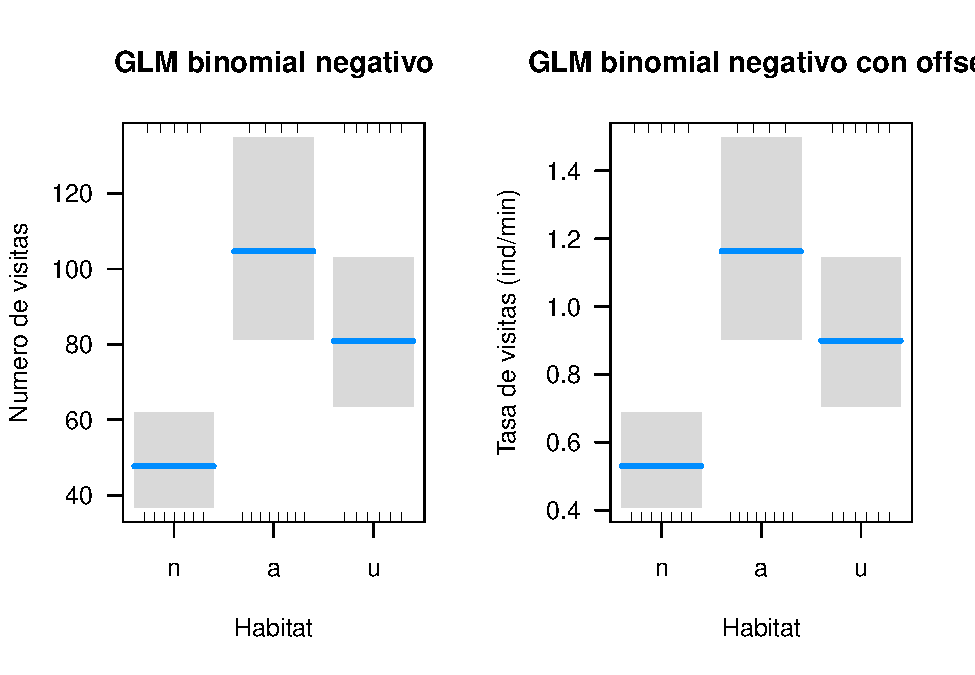
\includegraphics{_main_files/figure-latex/grafico glm BN-1.pdf}

\begin{Shaded}
\begin{Highlighting}[]
\KeywordTok{layout}\NormalTok{(}\DecValTok{1}\NormalTok{)}
\end{Highlighting}
\end{Shaded}

\hypertarget{modelo-lineal-general}{%
\section{Modelo lineal general}\label{modelo-lineal-general}}

Palacio et al.~(2014) estudiaron la selección natural mediada por aves frugívoras sobre rasgos de los frutos de \emph{Celtis tala} (\texttt{frutos\ Celtis\ 2013.txt}), incluyendo el diámetro (\texttt{diam}), peso (\texttt{peso}), concentración de azúcares (\texttt{az}), peso de pulpa (\texttt{pulpa}), peso de semilla (\texttt{sem}) y relación peso de pulpa/peso de semilla (\texttt{pulpa.sem}). Analizar qué factores explican el tamaño del fruto.

\begin{Shaded}
\begin{Highlighting}[]
\NormalTok{celtis <-}\StringTok{ }\KeywordTok{read.delim}\NormalTok{(}\StringTok{"frutos Celtis 2013.csv"}\NormalTok{, }\DataTypeTok{sep =} \StringTok{";"}\NormalTok{)}
\KeywordTok{str}\NormalTok{(celtis)}
\end{Highlighting}
\end{Shaded}

\begin{verbatim}
## 'data.frame':    617 obs. of  8 variables:
##  $ planta   : chr  "P1-10" "P1-10" "P1-10" "P1-10" ...
##  $ parche   : chr  "P1" "P1" "P1" "P1" ...
##  $ diam     : num  9.26 8.12 9.01 8.57 7.48 ...
##  $ peso     : num  0.414 0.291 0.387 0.339 0.222 0.307 0.318 0.35 0.259 0.294 ...
##  $ az       : num  18.5 21.5 18.5 23.5 16.5 ...
##  $ pulpa    : num  0.361 0.252 0.331 0.287 0.177 0.252 0.272 0.292 0.217 0.253 ...
##  $ sem      : num  0.0523 0.0393 0.0556 0.0519 0.0443 0.0555 0.0453 0.0581 0.0419 0.0417 ...
##  $ pulpa.sem: num  6.91 6.41 5.96 5.53 4 ...
\end{verbatim}

\begin{Shaded}
\begin{Highlighting}[]
\KeywordTok{pairs}\NormalTok{(celtis[, }\DecValTok{3}\OperatorTok{:}\DecValTok{7}\NormalTok{])}
\end{Highlighting}
\end{Shaded}

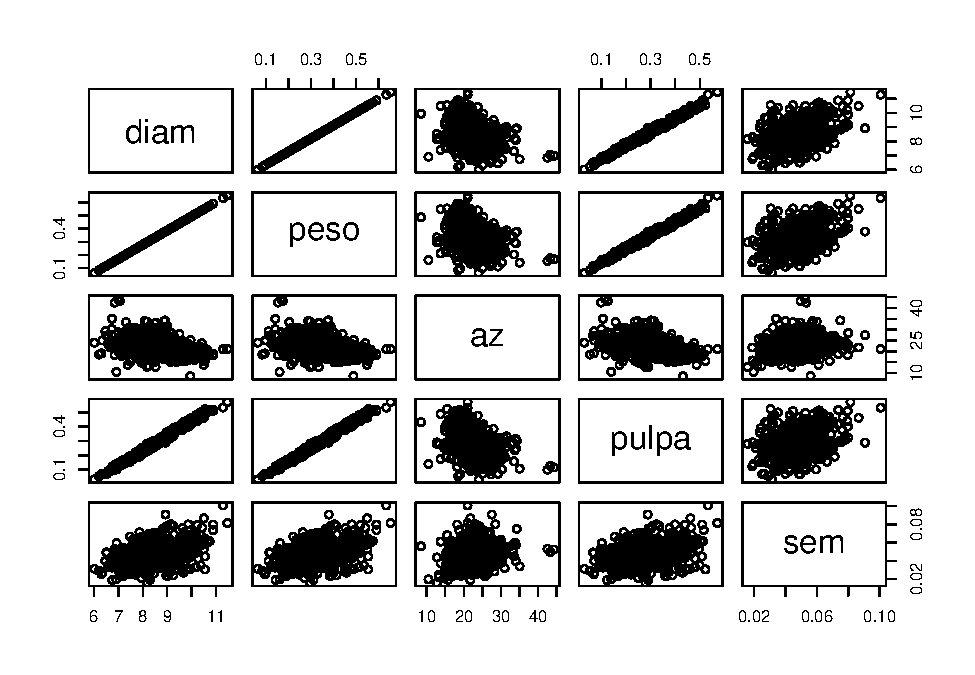
\includegraphics{_main_files/figure-latex/lm-1.pdf}

\begin{Shaded}
\begin{Highlighting}[]
\KeywordTok{round}\NormalTok{(}\KeywordTok{cor}\NormalTok{(celtis[, }\DecValTok{4}\OperatorTok{:}\DecValTok{7}\NormalTok{], }\DataTypeTok{use =} \StringTok{"complete.obs"}\NormalTok{), }\DecValTok{2}\NormalTok{)}
\end{Highlighting}
\end{Shaded}

\begin{verbatim}
##        peso    az pulpa  sem
## peso   1.00 -0.33  0.99 0.45
## az    -0.33  1.00 -0.37 0.20
## pulpa  0.99 -0.37  1.00 0.34
## sem    0.45  0.20  0.34 1.00
\end{verbatim}

\begin{Shaded}
\begin{Highlighting}[]
\KeywordTok{hist}\NormalTok{(celtis}\OperatorTok{$}\NormalTok{diam, }\DataTypeTok{xlab =} \StringTok{"Diametro (mm)"}\NormalTok{, }\DataTypeTok{ylab =} \StringTok{"Frecuencia"}\NormalTok{, }\DataTypeTok{main =} \StringTok{""}\NormalTok{)}
\end{Highlighting}
\end{Shaded}

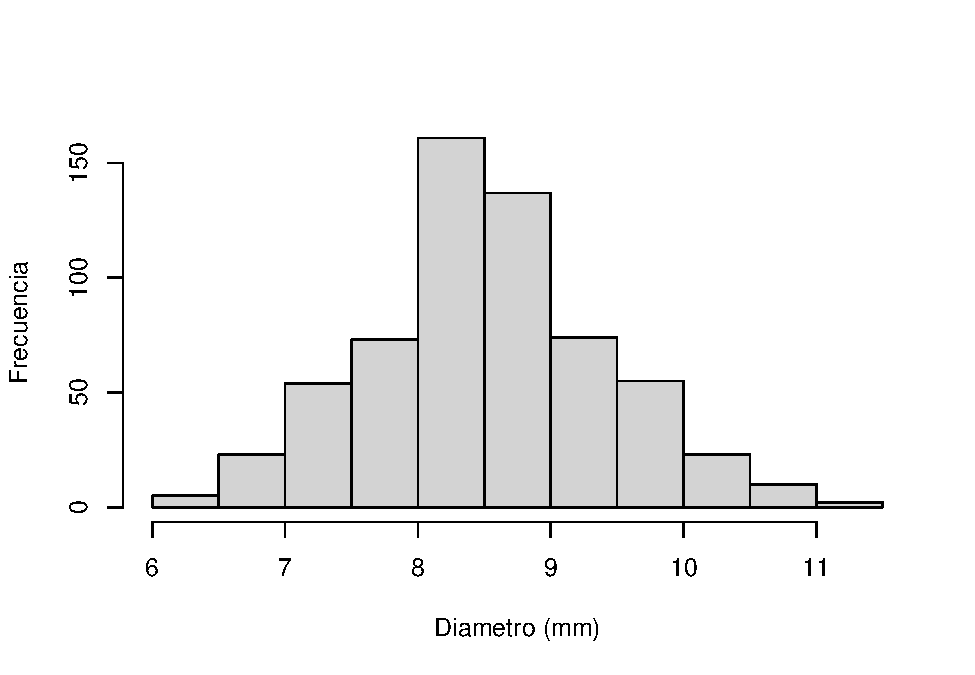
\includegraphics{_main_files/figure-latex/lm-2.pdf}

\begin{Shaded}
\begin{Highlighting}[]
\NormalTok{mlg <-}\StringTok{ }\KeywordTok{glm}\NormalTok{(diam }\OperatorTok{~}\StringTok{ }\NormalTok{az }\OperatorTok{+}\StringTok{ }\NormalTok{sem, }\DataTypeTok{family =}\NormalTok{ gaussian, }\DataTypeTok{data =}\NormalTok{ celtis)}
\KeywordTok{summary}\NormalTok{(mlg)}
\end{Highlighting}
\end{Shaded}

\begin{verbatim}
## 
## Call:
## glm(formula = diam ~ az + sem, family = gaussian, data = celtis)
## 
## Deviance Residuals: 
##      Min        1Q    Median        3Q       Max  
## -1.96247  -0.49375  -0.01025   0.46537   2.04017  
## 
## Coefficients:
##              Estimate Std. Error t value Pr(>|t|)    
## (Intercept)  8.750071   0.176681   49.52   <2e-16 ***
## az          -0.094204   0.006975  -13.51   <2e-16 ***
## sem         39.834317   2.400758   16.59   <2e-16 ***
## ---
## Signif. codes:  0 '***' 0.001 '**' 0.01 '*' 0.05 '.' 0.1 ' ' 1
## 
## (Dispersion parameter for gaussian family taken to be 0.4902039)
## 
##     Null deviance: 487.54  on 613  degrees of freedom
## Residual deviance: 299.51  on 611  degrees of freedom
##   (3 observations deleted due to missingness)
## AIC: 1309.7
## 
## Number of Fisher Scoring iterations: 2
\end{verbatim}

\hypertarget{glm-gamma}{%
\section{GLM Gamma}\label{glm-gamma}}

Allen et al.~(2015) analizaron el efecto de grandes carnívoros (\(Ursus americanus\) y \(Puma concolor\)) sobre la actividad de carroñeros. Registraron la duración media del evento de alimentación (\texttt{duration}) por carroñeros en sitios con cadáveres producto de pumas y sitios control donde se colocaron cadáveres colectados en la ruta (\texttt{trat}).

\begin{Shaded}
\begin{Highlighting}[]
\CommentTok{# Gráficos exploratorios }
\NormalTok{datos <-}\StringTok{ }\KeywordTok{read.table}\NormalTok{(}\StringTok{"puma.txt"}\NormalTok{, }\DataTypeTok{header =} \OtherTok{TRUE}\NormalTok{)}
\NormalTok{datos}\OperatorTok{$}\NormalTok{trat <-}\StringTok{ }\KeywordTok{as.factor}\NormalTok{(datos}\OperatorTok{$}\NormalTok{trat)}
\NormalTok{P <-}\StringTok{ }\KeywordTok{subset}\NormalTok{(datos, trat }\OperatorTok{==}\StringTok{ "Puma_Kill"}\NormalTok{) }
\NormalTok{C <-}\StringTok{ }\KeywordTok{subset}\NormalTok{(datos, trat }\OperatorTok{==}\StringTok{ "Control"}\NormalTok{) }
\KeywordTok{layout}\NormalTok{(}\KeywordTok{matrix}\NormalTok{(}\DecValTok{1}\OperatorTok{:}\DecValTok{2}\NormalTok{, }\DecValTok{1}\NormalTok{, }\DecValTok{2}\NormalTok{)) }
\KeywordTok{hist}\NormalTok{(P}\OperatorTok{$}\NormalTok{duration) }
\KeywordTok{hist}\NormalTok{(C}\OperatorTok{$}\NormalTok{duration) }
\end{Highlighting}
\end{Shaded}

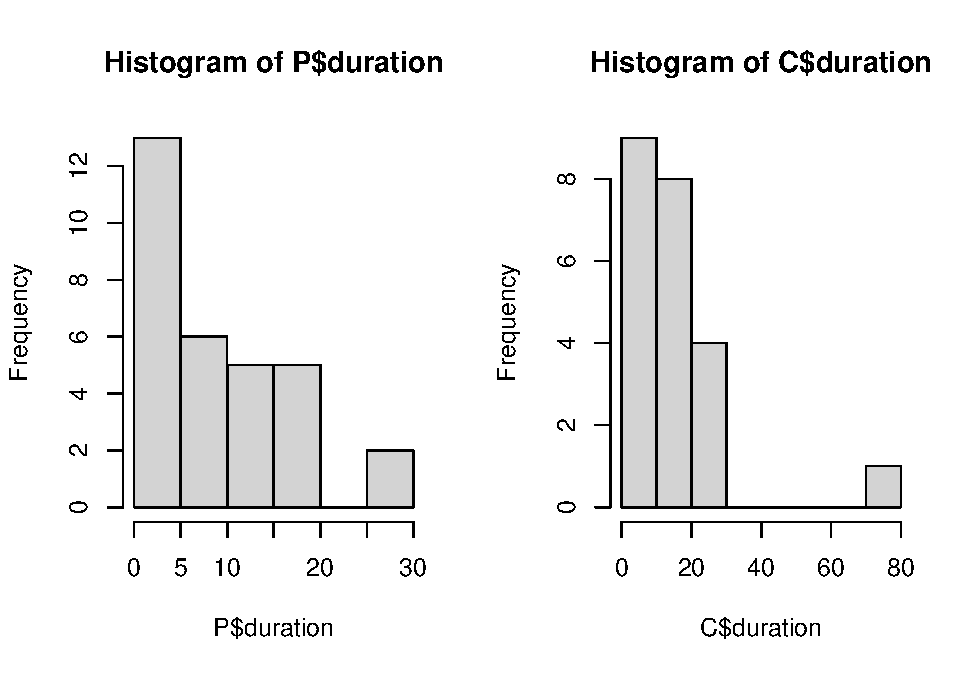
\includegraphics{_main_files/figure-latex/glm gamma-1.pdf}

\begin{Shaded}
\begin{Highlighting}[]
\KeywordTok{layout}\NormalTok{(}\DecValTok{1}\NormalTok{) }
\KeywordTok{boxplot}\NormalTok{(datos}\OperatorTok{$}\NormalTok{duration }\OperatorTok{~}\StringTok{ }\NormalTok{datos}\OperatorTok{$}\NormalTok{trat) }
\end{Highlighting}
\end{Shaded}

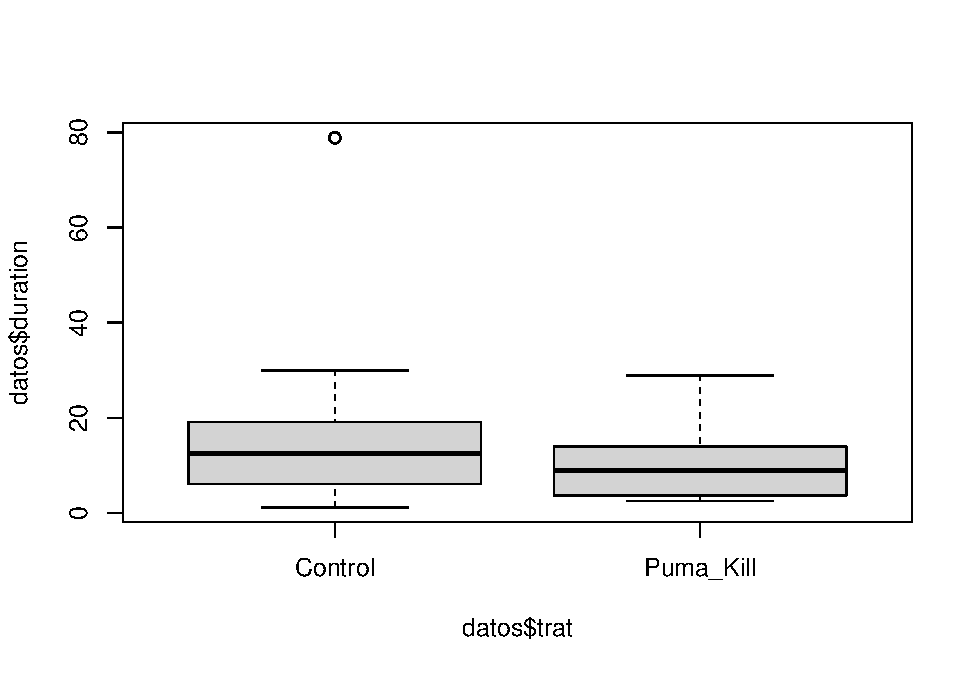
\includegraphics{_main_files/figure-latex/glm gamma-2.pdf}

\begin{Shaded}
\begin{Highlighting}[]
\CommentTok{# GLM Gamma }
\NormalTok{m.Gamma <-}\StringTok{ }\KeywordTok{glm}\NormalTok{(duration }\OperatorTok{~}\StringTok{ }\NormalTok{trat, }\DataTypeTok{family =}\NormalTok{ Gamma, }\DataTypeTok{data =}\NormalTok{ datos) }
\KeywordTok{summary}\NormalTok{(m.Gamma)}
\end{Highlighting}
\end{Shaded}

\begin{verbatim}
## 
## Call:
## glm(formula = duration ~ trat, family = Gamma, data = datos)
## 
## Deviance Residuals: 
##     Min       1Q   Median       3Q      Max  
## -1.7942  -0.8165  -0.1525   0.3143   2.2724  
## 
## Coefficients:
##               Estimate Std. Error t value Pr(>|t|)    
## (Intercept)    0.06639    0.01251   5.308 2.43e-06 ***
## tratPuma_Kill  0.03731    0.02067   1.805    0.077 .  
## ---
## Signif. codes:  0 '***' 0.001 '**' 0.01 '*' 0.05 '.' 0.1 ' ' 1
## 
## (Dispersion parameter for Gamma family taken to be 0.7808647)
## 
##     Null deviance: 35.695  on 52  degrees of freedom
## Residual deviance: 33.092  on 51  degrees of freedom
## AIC: 363.65
## 
## Number of Fisher Scoring iterations: 6
\end{verbatim}

\begin{Shaded}
\begin{Highlighting}[]
\CommentTok{# Comparaciones múltiples }
\KeywordTok{library}\NormalTok{(multcomp)}
\NormalTok{comp <-}\StringTok{ }\KeywordTok{glht}\NormalTok{(m.Gamma, }\KeywordTok{mcp}\NormalTok{(}\DataTypeTok{trat =} \StringTok{"Tukey"}\NormalTok{)) }
\KeywordTok{summary}\NormalTok{(comp)}
\end{Highlighting}
\end{Shaded}

\begin{verbatim}
## 
##   Simultaneous Tests for General Linear Hypotheses
## 
## Multiple Comparisons of Means: Tukey Contrasts
## 
## 
## Fit: glm(formula = duration ~ trat, family = Gamma, data = datos)
## 
## Linear Hypotheses:
##                          Estimate Std. Error z value Pr(>|z|)  
## Puma_Kill - Control == 0  0.03731    0.02067   1.805   0.0711 .
## ---
## Signif. codes:  0 '***' 0.001 '**' 0.01 '*' 0.05 '.' 0.1 ' ' 1
## (Adjusted p values reported -- single-step method)
\end{verbatim}

\hypertarget{actividades-1}{%
\section{Actividades}\label{actividades-1}}

\hypertarget{ejercicio-2.1}{%
\subsection{Ejercicio 2.1}\label{ejercicio-2.1}}

Identifique qué tipo de distribuciones de probabilidad utilizaría para las siguientes variables de respuesta. Justifique en cada caso.

\begin{enumerate}
\def\labelenumi{\alph{enumi}.}
\item
  Densidad de especies de plantas en parcelas de un bosque.
\item
  Probabilidad de detección de una especie de anfibio en charcas temporarias.
\item
  La tasa de crecimiento en pichones de una especie de ave.
\item
  El sexo en una especie de lagarto.
\end{enumerate}

\hypertarget{ejercicio-2.2}{%
\subsection{Ejercicio 2.2}\label{ejercicio-2.2}}

Se estimó la prevalencia del parásito \emph{Elaphostrongylus cervi} en ciervos colorados de granjas de España (\texttt{Tbdeer}). En cada granja (\texttt{Farm}) se muestreó un grupo de animales (\texttt{DeerSampledCervi}) y se registró si eran positivos para la enfermedad (\texttt{DeerPosCervi}). Además, se registraron variables de hábitat, como porcentaje de áreas abiertas (\texttt{OpenLand}), arbustos (\texttt{ScrubLand}) y plantaciones de pino (\texttt{PinePlantation}), densidad de plantas y árboles de \emph{Quercus} sp. (\texttt{QuercusPlants}, \texttt{QuercusTrees}). También se estimaron abundancias relativas de jabalí (\texttt{WildBoarIndex}) y ciervo colorado (\texttt{RedDeerIndex}), área del campo (\texttt{EstateSize}) y si el campo estaba cercado (1 = cercado, 0 = no cercado).

\begin{itemize}
\item
  Determine, cuáles de estas variables están involucradas en la prevalencia de la enfermedad.
\item
  Valide y grafique el modelo resultante.
\end{itemize}

\hypertarget{ejercicio-2.3}{%
\subsection{Ejercicio 2.3}\label{ejercicio-2.3}}

Simule un modelo lineal general (utilice la función \texttt{rnorm}) con dos variables (una con un efecto positivo y otra con un efecto negativo sobre la respuesta) y ajuste un modelo con las funciones \texttt{lm} y \texttt{glm}. Compare ambos modelos ¿Qué conclusión obtiene?

\hypertarget{ejercicio-2.4}{%
\subsubsection{Ejercicio 2.4}\label{ejercicio-2.4}}

Desarrolle un script para calcular el R\textsuperscript{2} de Tjur utilizando el GLM binomial de Solea.txt, donde:

\[R^{2}_{Tjur} = \frac{\sum \hat{p}(y = 1)}{n_1}\ + \frac{\sum \hat{p}(y = 0)}{n_0}\]

Corrobore el resultado con la función \texttt{r2\_tjur} del paquete \texttt{performance} ¿En qué situación hipotética el \(R^2\) vale 0?

\hypertarget{conteos-ii}{%
\section{Conteos II}\label{conteos-ii}}

\hypertarget{modelos-truncados-en-cero}{%
\subsection{Modelos truncados en cero}\label{modelos-truncados-en-cero}}

Santos et al.~(2011) estudiaron la probabilidad de persistencia de las carcasas de animales muertos en ruta (\texttt{Snakes.txt}). La variable respuesta es la cantidad de días que perduraban las carcasas sin ser removidas (\texttt{N\_days}). Las variables explicatorias son la longitud de cada especie (\texttt{Size\_cm}), la proporción de días con lluvia (\texttt{PDayRain}), las precipitaciones totales (\texttt{Tot\_Rain}), la temperatura diaria promedio (\texttt{Temp\_avg}), la identidad de la ruta que representa la intesidad del tráfico (\texttt{Road}; EN114 tiene alto tránsito, EN4 tiene tráfico medio, y EN370\_EN114\_4 tiene bajo tráfico), la ubicación en la ruta (\texttt{Road\_Loc}; L = asfalto, V = borde), la estación (\texttt{Season}), y la especie (\texttt{Species}).

\begin{Shaded}
\begin{Highlighting}[]
\CommentTok{# Analisis exploratorio}
\NormalTok{serp <-}\StringTok{ }\KeywordTok{read.table}\NormalTok{(}\StringTok{"Snakes.txt"}\NormalTok{, }\DataTypeTok{header =}\NormalTok{ T) }
\KeywordTok{str}\NormalTok{(serp)}
\end{Highlighting}
\end{Shaded}

\begin{verbatim}
## 'data.frame':    130 obs. of  11 variables:
##  $ ID      : int  2176 2448 2917 2927 2845 2849 2860 2760 2758 2764 ...
##  $ Road    : chr  "EN114" "EN114" "EN114" "EN114" ...
##  $ Month   : chr  "Jul" "Aug" "Oct" "Oct" ...
##  $ Season  : chr  "Summer" "Summer" "Autumn" "Autumn" ...
##  $ N_days  : int  4 1 4 2 1 1 2 1 2 2 ...
##  $ Species : chr  "Coluberhippocrepis" "Elaphescalaris" "Elaphescalaris" "Elaphescalaris" ...
##  $ Road_Loc: chr  "L" "L" "L" "L" ...
##  $ Size_cm : int  115 150 150 150 150 150 150 150 150 150 ...
##  $ PDayRain: num  0.75 0 1 1 0 0 0 0 0 0 ...
##  $ Tot_Rain: num  15 0 40.2 35.6 0 0 0 0 0 0 ...
##  $ Temp_avg: num  24.6 27.4 19.1 17.8 22.3 22.3 19.7 19.9 19.4 19.4 ...
\end{verbatim}

\begin{Shaded}
\begin{Highlighting}[]
\KeywordTok{plot}\NormalTok{(}\KeywordTok{table}\NormalTok{(serp}\OperatorTok{$}\NormalTok{N_days))}
\end{Highlighting}
\end{Shaded}

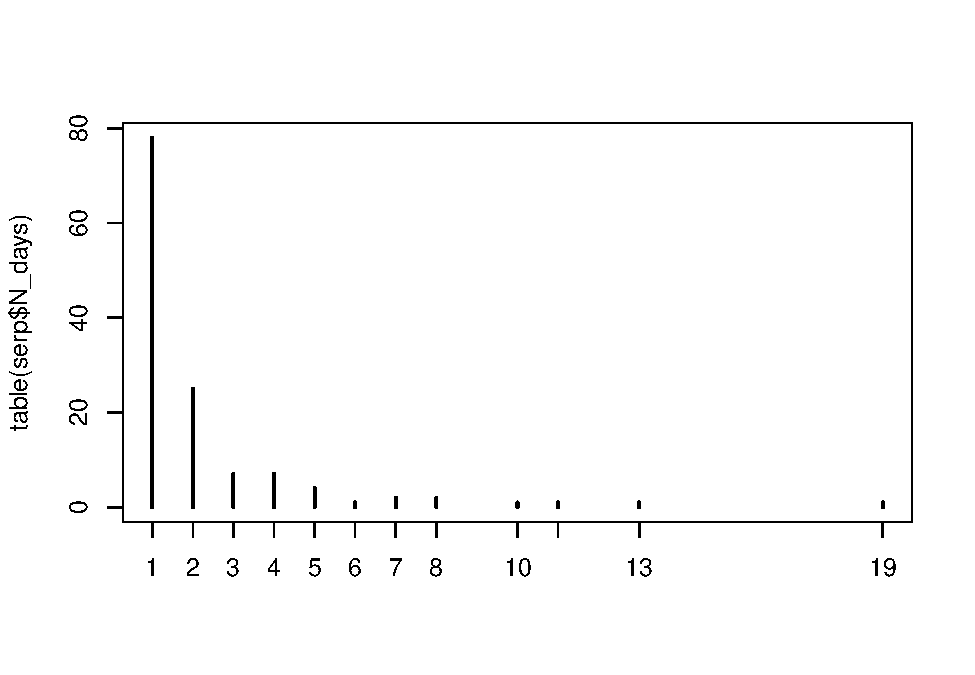
\includegraphics{_main_files/figure-latex/explo6-1.pdf}

\begin{Shaded}
\begin{Highlighting}[]
\KeywordTok{mean}\NormalTok{(serp}\OperatorTok{$}\NormalTok{N_days)}
\end{Highlighting}
\end{Shaded}

\begin{verbatim}
## [1] 2.2
\end{verbatim}

\begin{Shaded}
\begin{Highlighting}[]
\KeywordTok{pairs}\NormalTok{(serp[, }\KeywordTok{c}\NormalTok{(}\StringTok{"PDayRain"}\NormalTok{, }\StringTok{"Tot_Rain"}\NormalTok{, }\StringTok{"Temp_avg"}\NormalTok{)])}
\end{Highlighting}
\end{Shaded}

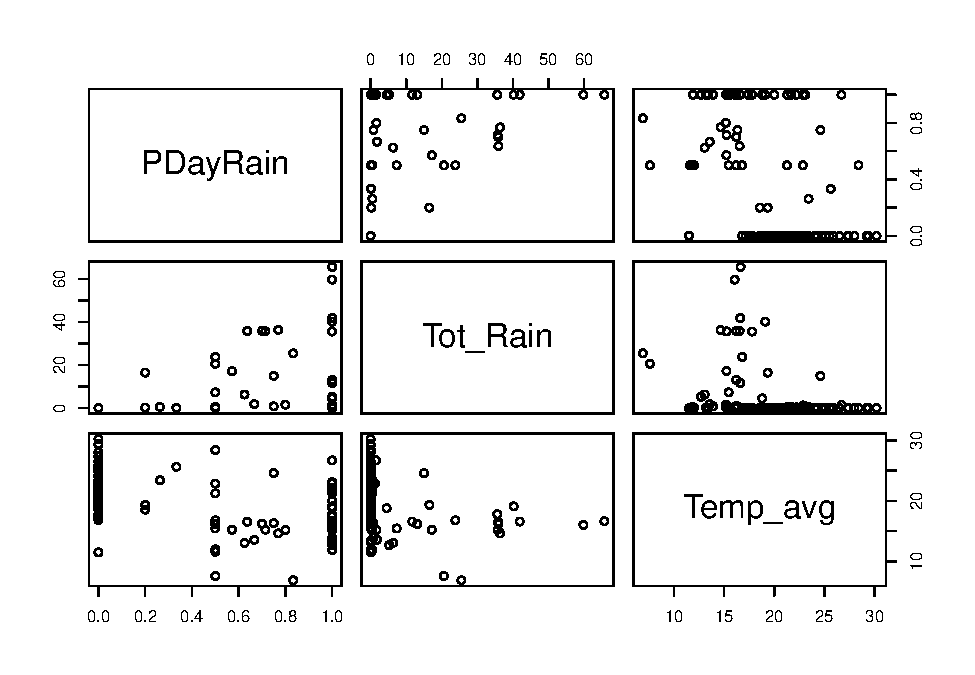
\includegraphics{_main_files/figure-latex/explo6-2.pdf}

\begin{Shaded}
\begin{Highlighting}[]
\KeywordTok{round}\NormalTok{(}\KeywordTok{cor}\NormalTok{(serp[, }\KeywordTok{c}\NormalTok{(}\StringTok{"PDayRain"}\NormalTok{, }\StringTok{"Tot_Rain"}\NormalTok{, }\StringTok{"Temp_avg"}\NormalTok{)]), }\DecValTok{2}\NormalTok{)}
\end{Highlighting}
\end{Shaded}

\begin{verbatim}
##          PDayRain Tot_Rain Temp_avg
## PDayRain     1.00     0.42     -0.5
## Tot_Rain     0.42     1.00     -0.3
## Temp_avg    -0.50    -0.30      1.0
\end{verbatim}

\begin{Shaded}
\begin{Highlighting}[]
\KeywordTok{boxplot}\NormalTok{(serp}\OperatorTok{$}\NormalTok{PDayRain }\OperatorTok{~}\StringTok{ }\NormalTok{serp}\OperatorTok{$}\NormalTok{Season)}
\end{Highlighting}
\end{Shaded}

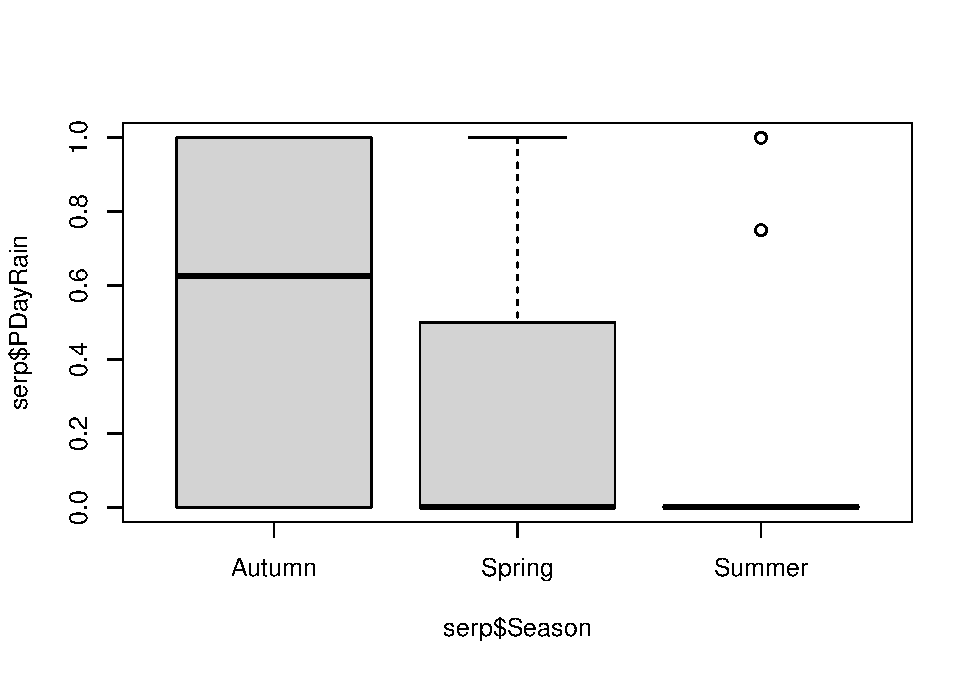
\includegraphics{_main_files/figure-latex/explo6-3.pdf}

\begin{Shaded}
\begin{Highlighting}[]
\KeywordTok{boxplot}\NormalTok{(serp}\OperatorTok{$}\NormalTok{Tot_Rain }\OperatorTok{~}\StringTok{ }\NormalTok{serp}\OperatorTok{$}\NormalTok{Season)}
\end{Highlighting}
\end{Shaded}

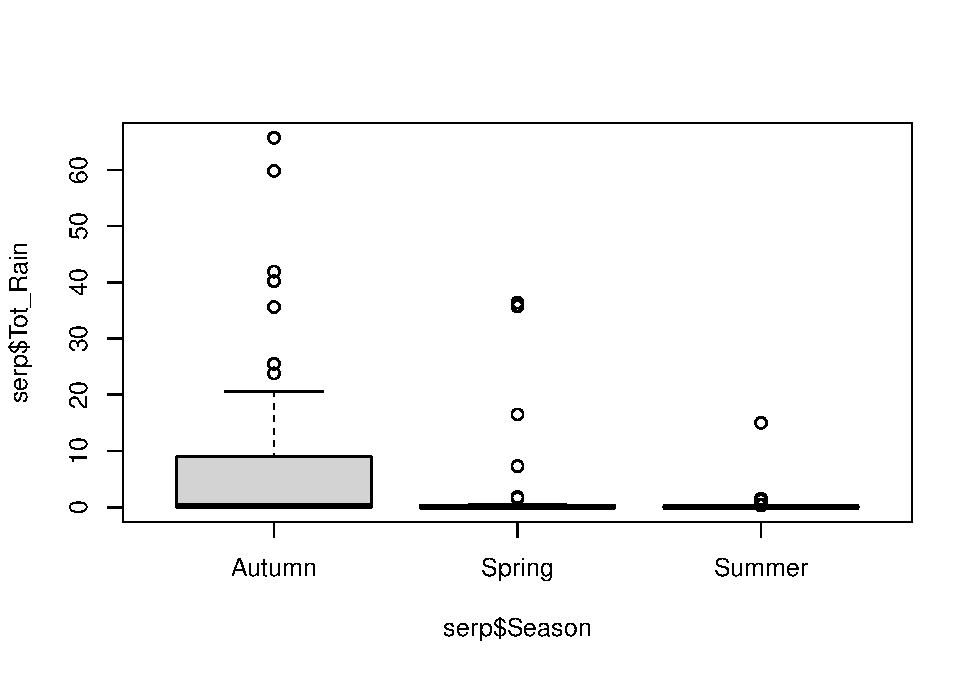
\includegraphics{_main_files/figure-latex/explo6-4.pdf}

\begin{Shaded}
\begin{Highlighting}[]
\KeywordTok{boxplot}\NormalTok{(serp}\OperatorTok{$}\NormalTok{Temp_avg }\OperatorTok{~}\StringTok{ }\NormalTok{serp}\OperatorTok{$}\NormalTok{Season)}
\end{Highlighting}
\end{Shaded}

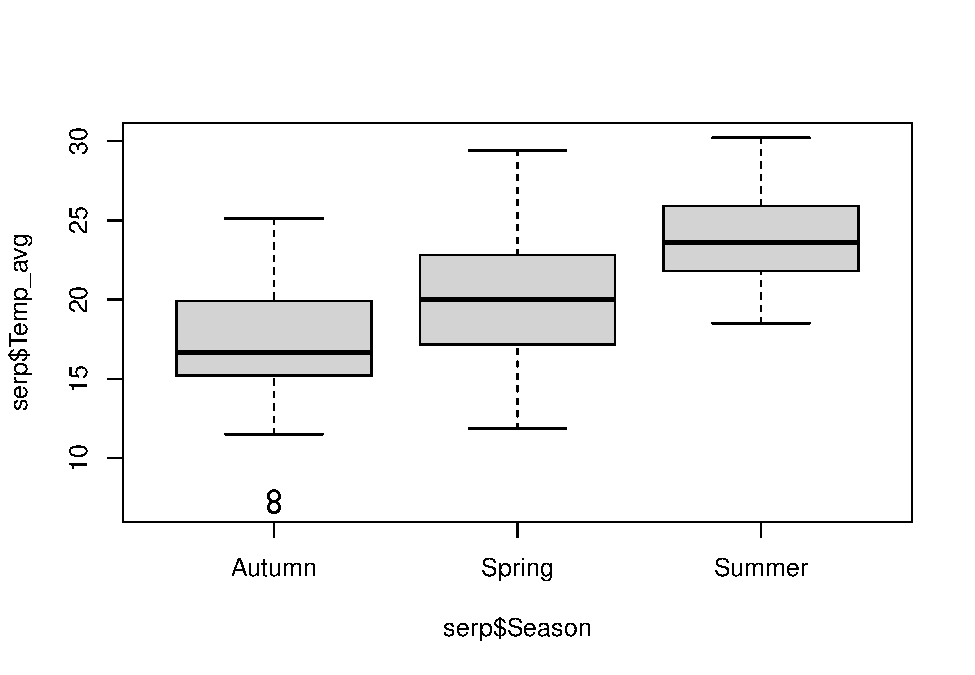
\includegraphics{_main_files/figure-latex/explo6-5.pdf}

\hypertarget{comparaciuxf3n-con-el-glm-poisson}{%
\subsubsection{Comparación con el GLM Poisson}\label{comparaciuxf3n-con-el-glm-poisson}}

\begin{Shaded}
\begin{Highlighting}[]
\NormalTok{m.pois <-}\StringTok{ }\KeywordTok{glm}\NormalTok{(N_days }\OperatorTok{~}\StringTok{ }\NormalTok{Size_cm }\OperatorTok{+}\StringTok{ }\NormalTok{PDayRain }\OperatorTok{+}\StringTok{ }\NormalTok{Tot_Rain }\OperatorTok{+}\StringTok{ }\NormalTok{Road }\OperatorTok{+}\StringTok{ }\NormalTok{Size_cm }\OperatorTok{+}\StringTok{ }\NormalTok{Road_Loc }\OperatorTok{+}\StringTok{ }\NormalTok{Size_cm}\OperatorTok{:}\NormalTok{PDayRain, }\DataTypeTok{family =}\NormalTok{ poisson, }\DataTypeTok{data =}\NormalTok{ serp)}
\KeywordTok{summary}\NormalTok{(m.pois)}
\end{Highlighting}
\end{Shaded}

\begin{verbatim}
## 
## Call:
## glm(formula = N_days ~ Size_cm + PDayRain + Tot_Rain + Road + 
##     Size_cm + Road_Loc + Size_cm:PDayRain, family = poisson, 
##     data = serp)
## 
## Deviance Residuals: 
##     Min       1Q   Median       3Q      Max  
## -2.0869  -0.7901  -0.4193   0.2448   5.9495  
## 
## Coefficients:
##                    Estimate Std. Error z value Pr(>|z|)    
## (Intercept)       -0.114527   0.463263  -0.247 0.804739    
## Size_cm            0.004782   0.002965   1.613 0.106848    
## PDayRain           0.957714   0.768545   1.246 0.212713    
## Tot_Rain           0.022763   0.003797   5.994 2.04e-09 ***
## RoadEN370_EN114_4 -0.146154   0.172785  -0.846 0.397626    
## RoadEN4           -0.352271   0.147973  -2.381 0.017282 *  
## Road_LocV          0.530610   0.158214   3.354 0.000797 ***
## Size_cm:PDayRain  -0.006869   0.005161  -1.331 0.183215    
## ---
## Signif. codes:  0 '***' 0.001 '**' 0.01 '*' 0.05 '.' 0.1 ' ' 1
## 
## (Dispersion parameter for poisson family taken to be 1)
## 
##     Null deviance: 226.38  on 129  degrees of freedom
## Residual deviance: 166.85  on 122  degrees of freedom
## AIC: 498.68
## 
## Number of Fisher Scoring iterations: 5
\end{verbatim}

\hypertarget{glm-poisson-truncado-en-cero}{%
\subsubsection{GLM Poisson truncado en cero}\label{glm-poisson-truncado-en-cero}}

\begin{Shaded}
\begin{Highlighting}[]
\KeywordTok{library}\NormalTok{(VGAM)}
\end{Highlighting}
\end{Shaded}

\begin{verbatim}
## Warning: package 'VGAM' was built under R version 4.0.5
\end{verbatim}

\begin{verbatim}
## Loading required package: stats4
\end{verbatim}

\begin{verbatim}
## Loading required package: splines
\end{verbatim}

\begin{verbatim}
## 
## Attaching package: 'VGAM'
\end{verbatim}

\begin{verbatim}
## The following object is masked from 'package:car':
## 
##     logit
\end{verbatim}

\begin{verbatim}
## The following objects are masked from 'package:psych':
## 
##     fisherz, logistic, logit
\end{verbatim}

\begin{Shaded}
\begin{Highlighting}[]
\NormalTok{m.pois.trun <-}\StringTok{ }\KeywordTok{vglm}\NormalTok{(N_days }\OperatorTok{~}\StringTok{ }\NormalTok{Size_cm }\OperatorTok{+}\StringTok{ }\NormalTok{PDayRain }\OperatorTok{+}\StringTok{ }\NormalTok{Tot_Rain }\OperatorTok{+}\StringTok{ }\NormalTok{Road }\OperatorTok{+}\StringTok{ }\NormalTok{Size_cm }\OperatorTok{+}\StringTok{ }\NormalTok{Road_Loc }\OperatorTok{+}\StringTok{ }\NormalTok{Size_cm}\OperatorTok{:}\NormalTok{PDayRain, }\DataTypeTok{family =}\NormalTok{ pospoisson, }\DataTypeTok{control =}  \KeywordTok{vglm.control}\NormalTok{(}\DataTypeTok{maxit =} \DecValTok{100}\NormalTok{), }\DataTypeTok{data =}\NormalTok{ serp)}
\KeywordTok{summary}\NormalTok{(m.pois.trun)}
\end{Highlighting}
\end{Shaded}

\begin{verbatim}
## 
## Call:
## vglm(formula = N_days ~ Size_cm + PDayRain + Tot_Rain + Road + 
##     Size_cm + Road_Loc + Size_cm:PDayRain, family = pospoisson, 
##     data = serp, control = vglm.control(maxit = 100))
## 
## Coefficients: 
##                    Estimate Std. Error z value Pr(>|z|)    
## (Intercept)       -1.214880   0.764099  -1.590  0.11185    
## Size_cm            0.009725   0.004830   2.014  0.04406 *  
## PDayRain           1.782494   1.097674   1.624  0.10440    
## Tot_Rain           0.028863   0.004270   6.760 1.38e-11 ***
## RoadEN370_EN114_4 -0.217333   0.225081  -0.966  0.33425    
## RoadEN4           -0.558705   0.181936  -3.071  0.00213 ** 
## Road_LocV          0.811896   0.200842   4.042 5.29e-05 ***
## Size_cm:PDayRain  -0.012131   0.007245  -1.674  0.09404 .  
## ---
## Signif. codes:  0 '***' 0.001 '**' 0.01 '*' 0.05 '.' 0.1 ' ' 1
## 
## Name of linear predictor: loglink(lambda) 
## 
## Log-likelihood: -211.1832 on 122 degrees of freedom
## 
## Number of Fisher scoring iterations: 5 
## 
## No Hauck-Donner effect found in any of the estimates
\end{verbatim}

\hypertarget{glm-binomial-negativo-truncado-en-cero}{%
\subsubsection{GLM binomial negativo truncado en cero}\label{glm-binomial-negativo-truncado-en-cero}}

\begin{Shaded}
\begin{Highlighting}[]
\NormalTok{m.nb.trun <-}\StringTok{ }\KeywordTok{vglm}\NormalTok{(N_days }\OperatorTok{~}\StringTok{ }\NormalTok{Size_cm }\OperatorTok{+}\StringTok{ }\NormalTok{PDayRain }\OperatorTok{+}\StringTok{ }\NormalTok{Tot_Rain }\OperatorTok{+}\StringTok{ }\NormalTok{Road }\OperatorTok{+}\StringTok{ }\NormalTok{Size_cm }\OperatorTok{+}\StringTok{ }\NormalTok{Road_Loc }\OperatorTok{+}\StringTok{ }\NormalTok{Size_cm}\OperatorTok{:}\NormalTok{PDayRain, }\DataTypeTok{family =}\NormalTok{ posnegbinomial, }\DataTypeTok{control =}  \KeywordTok{vglm.control}\NormalTok{(}\DataTypeTok{maxit =} \DecValTok{100}\NormalTok{), }\DataTypeTok{data =}\NormalTok{ serp)}
\end{Highlighting}
\end{Shaded}

\begin{verbatim}
## Warning in slot(family, "linkinv")(eta, extra = extra): estimates of 'size' are very
## small. Taking evasive action.
\end{verbatim}

\begin{verbatim}
## Warning in slot(family, "validparams")(eta, y = y, extra = extra): parameter 'size' has
## very large values relative to 'munb'; try fitting a positive-Poisson model instead.
\end{verbatim}

\begin{verbatim}
## Warning in eval(slot(family, "deriv")): solution near the boundary; either there is no
## need to fit a positive NBD or the distribution is centred on the value 1
\end{verbatim}

\begin{verbatim}
## Warning in slot(family, "validparams")(eta, y, extra = extra): parameter 'size' has very
## large values relative to 'munb'; try fitting a positive-Poisson model instead.
\end{verbatim}

\begin{verbatim}
## Warning in vglm.fitter(x = x, y = y, w = w, offset = offset, Xm2 = Xm2, : iterations
## terminated because half-step sizes are very small
\end{verbatim}

\begin{verbatim}
## Warning in vglm.fitter(x = x, y = y, w = w, offset = offset, Xm2 = Xm2, : some quantities
## such as z, residuals, SEs may be inaccurate due to convergence at a half-step
\end{verbatim}

\begin{Shaded}
\begin{Highlighting}[]
\KeywordTok{summary}\NormalTok{(m.nb.trun)}
\end{Highlighting}
\end{Shaded}

\begin{verbatim}
## Warning in eval(expr): solution near the boundary; either there is no need to fit a
## positive NBD or the distribution is centred on the value 1
\end{verbatim}

\begin{verbatim}
## Warning in eval(expr): solution near the boundary; either there is no need to fit a
## positive NBD or the distribution is centred on the value 1

## Warning in eval(expr): solution near the boundary; either there is no need to fit a
## positive NBD or the distribution is centred on the value 1

## Warning in eval(expr): solution near the boundary; either there is no need to fit a
## positive NBD or the distribution is centred on the value 1

## Warning in eval(expr): solution near the boundary; either there is no need to fit a
## positive NBD or the distribution is centred on the value 1

## Warning in eval(expr): solution near the boundary; either there is no need to fit a
## positive NBD or the distribution is centred on the value 1

## Warning in eval(expr): solution near the boundary; either there is no need to fit a
## positive NBD or the distribution is centred on the value 1

## Warning in eval(expr): solution near the boundary; either there is no need to fit a
## positive NBD or the distribution is centred on the value 1

## Warning in eval(expr): solution near the boundary; either there is no need to fit a
## positive NBD or the distribution is centred on the value 1

## Warning in eval(expr): solution near the boundary; either there is no need to fit a
## positive NBD or the distribution is centred on the value 1

## Warning in eval(expr): solution near the boundary; either there is no need to fit a
## positive NBD or the distribution is centred on the value 1

## Warning in eval(expr): solution near the boundary; either there is no need to fit a
## positive NBD or the distribution is centred on the value 1

## Warning in eval(expr): solution near the boundary; either there is no need to fit a
## positive NBD or the distribution is centred on the value 1

## Warning in eval(expr): solution near the boundary; either there is no need to fit a
## positive NBD or the distribution is centred on the value 1

## Warning in eval(expr): solution near the boundary; either there is no need to fit a
## positive NBD or the distribution is centred on the value 1

## Warning in eval(expr): solution near the boundary; either there is no need to fit a
## positive NBD or the distribution is centred on the value 1

## Warning in eval(expr): solution near the boundary; either there is no need to fit a
## positive NBD or the distribution is centred on the value 1

## Warning in eval(expr): solution near the boundary; either there is no need to fit a
## positive NBD or the distribution is centred on the value 1

## Warning in eval(expr): solution near the boundary; either there is no need to fit a
## positive NBD or the distribution is centred on the value 1
\end{verbatim}

\begin{verbatim}
## 
## Call:
## vglm(formula = N_days ~ Size_cm + PDayRain + Tot_Rain + Road + 
##     Size_cm + Road_Loc + Size_cm:PDayRain, family = posnegbinomial, 
##     data = serp, control = vglm.control(maxit = 100))
## 
## Coefficients: 
##                     Estimate Std. Error  z value Pr(>|z|)    
## (Intercept):1     -18.650956   9.622924       NA       NA    
## (Intercept):2     -19.201942   0.087878 -218.508   <2e-16 ***
## Size_cm             0.006975   0.062006    0.112    0.910    
## PDayRain            1.196235  18.692101    0.064    0.949    
## Tot_Rain            0.067164   0.117128    0.573    0.566    
## RoadEN370_EN114_4  -0.276550   4.059935   -0.068    0.946    
## RoadEN4            -0.558499   3.643634   -0.153    0.878    
## Road_LocV           1.072722   3.817984    0.281    0.779    
## Size_cm:PDayRain   -0.009605   0.126436   -0.076    0.939    
## ---
## Signif. codes:  0 '***' 0.001 '**' 0.01 '*' 0.05 '.' 0.1 ' ' 1
## 
## Names of linear predictors: loglink(munb), loglink(size)
## 
## Log-likelihood: -186.7285 on 251 degrees of freedom
## 
## Number of Fisher scoring iterations: 3 
## 
## Warning: Hauck-Donner effect detected in the following estimate(s):
## '(Intercept):1'
\end{verbatim}

\hypertarget{comparaciuxf3n-de-coeficientes-entre-modelos}{%
\subsubsection{Comparación de coeficientes entre modelos}\label{comparaciuxf3n-de-coeficientes-entre-modelos}}

\begin{Shaded}
\begin{Highlighting}[]
\KeywordTok{data.frame}\NormalTok{(}\DataTypeTok{coef.Poisson =} \KeywordTok{summary}\NormalTok{(m.pois)}\OperatorTok{$}\NormalTok{coeff[, }\DecValTok{1}\NormalTok{], }
           \DataTypeTok{coef.Poisson.truncado =} \KeywordTok{summary}\NormalTok{(m.pois.trun)}\OperatorTok{@}\NormalTok{coef3[, }\DecValTok{1}\NormalTok{])}
\end{Highlighting}
\end{Shaded}

\begin{verbatim}
##                   coef.Poisson coef.Poisson.truncado
## (Intercept)       -0.114527460          -1.214879652
## Size_cm            0.004781715           0.009724801
## PDayRain           0.957714141           1.782494406
## Tot_Rain           0.022763117           0.028863331
## RoadEN370_EN114_4 -0.146153654          -0.217333044
## RoadEN4           -0.352270790          -0.558704924
## Road_LocV          0.530609962           0.811896312
## Size_cm:PDayRain  -0.006868709          -0.012131485
\end{verbatim}

\hypertarget{modelos-inflados-en-ceros}{%
\subsection{Modelos inflados en ceros}\label{modelos-inflados-en-ceros}}

Hemmingsen et al.~(2005) analizaron las infecciones por \emph{Trypanosoma} en bacalaos (\emph{Gadus morhua}) durante cruceros anuales en la costa norte de Noruega (\texttt{ParasiteCod.txt}). La variable respuesta es la prevalencia de parásitos (\texttt{Prevalence}). Posibles variables explicatorias son el año (\texttt{Year}), el área (\texttt{Area}) y la profundidad de captura (\texttt{Depth}).

\begin{Shaded}
\begin{Highlighting}[]
\CommentTok{# Análisis exploratorio}
\NormalTok{parasitos <-}\StringTok{ }\KeywordTok{read.table}\NormalTok{(}\StringTok{"ParasiteCod.txt"}\NormalTok{, }\DataTypeTok{header =}\NormalTok{ T) }
\KeywordTok{str}\NormalTok{(parasitos)}
\end{Highlighting}
\end{Shaded}

\begin{verbatim}
## 'data.frame':    1254 obs. of  11 variables:
##  $ Sample    : int  1 2 3 4 5 6 7 8 9 10 ...
##  $ Intensity : int  0 0 0 0 0 0 0 0 0 0 ...
##  $ Prevalence: int  0 0 0 0 0 0 0 0 0 0 ...
##  $ Year      : int  1999 1999 1999 1999 1999 1999 1999 1999 1999 1999 ...
##  $ Depth     : int  220 220 220 220 220 220 220 194 194 194 ...
##  $ Weight    : int  148 144 146 138 40 68 52 3848 2576 1972 ...
##  $ Length    : int  26 26 27 26 17 20 19 77 67 60 ...
##  $ Sex       : int  0 0 0 0 0 0 0 0 0 0 ...
##  $ Stage     : int  0 0 0 0 0 0 0 0 0 0 ...
##  $ Age       : int  0 0 0 0 0 0 0 0 0 0 ...
##  $ Area      : int  2 2 2 2 2 2 2 3 3 3 ...
\end{verbatim}

\begin{Shaded}
\begin{Highlighting}[]
\KeywordTok{plot}\NormalTok{(}\KeywordTok{table}\NormalTok{(parasitos}\OperatorTok{$}\NormalTok{Intensity))}
\end{Highlighting}
\end{Shaded}

\includegraphics{_main_files/figure-latex/explo7-1.pdf}

\begin{Shaded}
\begin{Highlighting}[]
\KeywordTok{table}\NormalTok{(parasitos}\OperatorTok{$}\NormalTok{Intensity)[}\DecValTok{1}\NormalTok{] }\CommentTok{# Número de ceros observados}
\end{Highlighting}
\end{Shaded}

\begin{verbatim}
##   0 
## 654
\end{verbatim}

\begin{Shaded}
\begin{Highlighting}[]
\CommentTok{# Ajuste de distribución a los datos}
\NormalTok{xIntensity <-}\StringTok{ }\KeywordTok{mean}\NormalTok{(parasitos}\OperatorTok{$}\NormalTok{Intensity, }\DataTypeTok{na.rm =} \OtherTok{TRUE}\NormalTok{)}
\NormalTok{sim.pois <-}\StringTok{ }\KeywordTok{dpois}\NormalTok{(}\DataTypeTok{x =} \DecValTok{0}\OperatorTok{:}\KeywordTok{max}\NormalTok{(parasitos}\OperatorTok{$}\NormalTok{Intensity, }\DataTypeTok{na.rm =} \OtherTok{TRUE}\NormalTok{), }\DataTypeTok{lambda =}\NormalTok{ xIntensity)}
\NormalTok{ndatos <-}\StringTok{ }\KeywordTok{length}\NormalTok{(}\KeywordTok{na.omit}\NormalTok{(parasitos}\OperatorTok{$}\NormalTok{Intensity))}
\NormalTok{random.sample.pois <-}\StringTok{ }\KeywordTok{rpois}\NormalTok{(}\DataTypeTok{n =}\NormalTok{ ndatos, }\DataTypeTok{lambda =}\NormalTok{ xIntensity)}
\KeywordTok{plot}\NormalTok{(}\KeywordTok{table}\NormalTok{(random.sample.pois))}
\end{Highlighting}
\end{Shaded}

\includegraphics{_main_files/figure-latex/explo7-2.pdf}

\begin{Shaded}
\begin{Highlighting}[]
\KeywordTok{dpois}\NormalTok{(}\DataTypeTok{x =} \DecValTok{0}\NormalTok{, }\DataTypeTok{lambda =}\NormalTok{ xIntensity) }\CommentTok{# Probabilidad de observar un cero}
\end{Highlighting}
\end{Shaded}

\begin{verbatim}
## [1] 0.002064314
\end{verbatim}

\begin{Shaded}
\begin{Highlighting}[]
\KeywordTok{table}\NormalTok{(random.sample.pois) }\CommentTok{# Numero de ceros esperados}
\end{Highlighting}
\end{Shaded}

\begin{verbatim}
## random.sample.pois
##   1   2   3   4   5   6   7   8   9  10  11  12  13 
##  17  56 109 153 187 171 170 122  96  54  37  20   5
\end{verbatim}

\hypertarget{modelos-de-dos-partes-o-valla-zap-y-zanb}{%
\subsubsection{Modelos de dos partes o ``valla'' (ZAP y ZANB)}\label{modelos-de-dos-partes-o-valla-zap-y-zanb}}

\begin{Shaded}
\begin{Highlighting}[]
\CommentTok{# La primera parte de la formula contiene las covariables para el proceso de conteo, la segunda parte contiene las covariables para la probabilidad de los falsos ceros.}
\KeywordTok{library}\NormalTok{(pscl)}
\end{Highlighting}
\end{Shaded}

\begin{verbatim}
## Warning: package 'pscl' was built under R version 4.0.5
\end{verbatim}

\begin{verbatim}
## Classes and Methods for R developed in the
## Political Science Computational Laboratory
## Department of Political Science
## Stanford University
## Simon Jackman
## hurdle and zeroinfl functions by Achim Zeileis
\end{verbatim}

\begin{Shaded}
\begin{Highlighting}[]
\NormalTok{ZAP <-}\StringTok{ }\KeywordTok{hurdle}\NormalTok{(Intensity }\OperatorTok{~}\StringTok{ }\NormalTok{Depth }\OperatorTok{|}\StringTok{ }\NormalTok{Length }\OperatorTok{+}\StringTok{ }\NormalTok{Depth, }\DataTypeTok{dist =} \StringTok{"poisson"}\NormalTok{, }
\DataTypeTok{link =} \StringTok{"logit"}\NormalTok{, }\DataTypeTok{data =}\NormalTok{ parasitos)}
\KeywordTok{summary}\NormalTok{(ZAP)}
\end{Highlighting}
\end{Shaded}

\begin{verbatim}
## 
## Call:
## hurdle(formula = Intensity ~ Depth | Length + Depth, data = parasitos, dist = "poisson", 
##     link = "logit")
## 
## Pearson residuals:
##     Min      1Q  Median      3Q     Max 
## -1.3420 -0.8995 -0.6450 -0.2622 32.6701 
## 
## Count model coefficients (truncated poisson with log link):
##              Estimate Std. Error z value Pr(>|z|)    
## (Intercept) 1.7740079  0.0412390   43.02   <2e-16 ***
## Depth       0.0041351  0.0001857   22.27   <2e-16 ***
## Zero hurdle model coefficients (binomial with logit link):
##               Estimate Std. Error z value Pr(>|z|)    
## (Intercept) -1.6523797  0.2870146  -5.757 8.56e-09 ***
## Length       0.0039426  0.0042165   0.935     0.35    
## Depth        0.0070509  0.0008584   8.214  < 2e-16 ***
## ---
## Signif. codes:  0 '***' 0.001 '**' 0.01 '*' 0.05 '.' 0.1 ' ' 1 
## 
## Number of iterations in BFGS optimization: 10 
## Log-likelihood: -8542 on 5 Df
\end{verbatim}

\begin{Shaded}
\begin{Highlighting}[]
\NormalTok{ZANB <-}\StringTok{ }\KeywordTok{hurdle}\NormalTok{(Intensity }\OperatorTok{~}\StringTok{ }\NormalTok{Depth }\OperatorTok{|}\StringTok{ }\NormalTok{Length }\OperatorTok{+}\StringTok{ }\NormalTok{Depth, }\DataTypeTok{dist =} \StringTok{"negbin"}\NormalTok{, }
\DataTypeTok{link =} \StringTok{"logit"}\NormalTok{, }\DataTypeTok{data =}\NormalTok{ parasitos)}
\KeywordTok{summary}\NormalTok{(ZANB)}
\end{Highlighting}
\end{Shaded}

\begin{verbatim}
## 
## Call:
## hurdle(formula = Intensity ~ Depth | Length + Depth, data = parasitos, dist = "negbin", 
##     link = "logit")
## 
## Pearson residuals:
##     Min      1Q  Median      3Q     Max 
## -0.4350 -0.3729 -0.3281 -0.1126 16.3175 
## 
## Count model coefficients (truncated negbin with log link):
##              Estimate Std. Error z value Pr(>|z|)    
## (Intercept) -0.415345   0.844211  -0.492 0.622725    
## Depth        0.006271   0.001537   4.080 4.51e-05 ***
## Log(theta)  -3.019216   0.867902  -3.479 0.000504 ***
## Zero hurdle model coefficients (binomial with logit link):
##               Estimate Std. Error z value Pr(>|z|)    
## (Intercept) -1.6523797  0.2870146  -5.757 8.56e-09 ***
## Length       0.0039426  0.0042165   0.935     0.35    
## Depth        0.0070509  0.0008584   8.214  < 2e-16 ***
## ---
## Signif. codes:  0 '***' 0.001 '**' 0.01 '*' 0.05 '.' 0.1 ' ' 1 
## 
## Theta: count = 0.0488
## Number of iterations in BFGS optimization: 16 
## Log-likelihood: -2559 on 6 Df
\end{verbatim}

\hypertarget{comparaciuxf3n-de-zap-y-zanb}{%
\subsubsection{Comparación de ZAP y ZANB}\label{comparaciuxf3n-de-zap-y-zanb}}

\begin{Shaded}
\begin{Highlighting}[]
\KeywordTok{library}\NormalTok{(lmtest)}
\end{Highlighting}
\end{Shaded}

\begin{verbatim}
## Loading required package: zoo
\end{verbatim}

\begin{verbatim}
## 
## Attaching package: 'zoo'
\end{verbatim}

\begin{verbatim}
## The following objects are masked from 'package:base':
## 
##     as.Date, as.Date.numeric
\end{verbatim}

\begin{verbatim}
## 
## Attaching package: 'lmtest'
\end{verbatim}

\begin{verbatim}
## The following object is masked from 'package:VGAM':
## 
##     lrtest
\end{verbatim}

\begin{Shaded}
\begin{Highlighting}[]
\KeywordTok{lrtest}\NormalTok{(ZAP, ZANB) }\CommentTok{# Test de razón de verosimilitud}
\end{Highlighting}
\end{Shaded}

\begin{verbatim}
## Likelihood ratio test
## 
## Model 1: Intensity ~ Depth | Length + Depth
## Model 2: Intensity ~ Depth | Length + Depth
##   #Df  LogLik Df Chisq Pr(>Chisq)    
## 1   5 -8542.3                        
## 2   6 -2559.4  1 11966  < 2.2e-16 ***
## ---
## Signif. codes:  0 '***' 0.001 '**' 0.01 '*' 0.05 '.' 0.1 ' ' 1
\end{verbatim}

\begin{Shaded}
\begin{Highlighting}[]
\KeywordTok{AIC}\NormalTok{(ZAP, ZANB)}
\end{Highlighting}
\end{Shaded}

\begin{verbatim}
##      df      AIC
## ZAP   5 17094.58
## ZANB  6  5130.85
\end{verbatim}

\hypertarget{validaciuxf3n}{%
\subsubsection{Validación}\label{validaciuxf3n}}

\begin{Shaded}
\begin{Highlighting}[]
\NormalTok{resid <-}\StringTok{ }\KeywordTok{residuals}\NormalTok{(ZANB, }\DataTypeTok{type =} \StringTok{"pearson"}\NormalTok{)}
\KeywordTok{plot}\NormalTok{(resid, }\KeywordTok{predict}\NormalTok{(ZANB), }\DataTypeTok{xlab =} \StringTok{"Residuos"}\NormalTok{, }\DataTypeTok{ylab =} \StringTok{"Predichos"}\NormalTok{)}
\end{Highlighting}
\end{Shaded}

\includegraphics{_main_files/figure-latex/validacion ZANB-1.pdf}

\hypertarget{interpretaciuxf3n-y-gruxe1ficos-del-modelo}{%
\subsubsection{Interpretación y gráficos del modelo}\label{interpretaciuxf3n-y-gruxe1ficos-del-modelo}}

\begin{Shaded}
\begin{Highlighting}[]
\CommentTok{# Proceso de falsos ceros}
\NormalTok{Depth <-}\StringTok{ }\KeywordTok{seq}\NormalTok{(}\KeywordTok{min}\NormalTok{(parasitos}\OperatorTok{$}\NormalTok{Depth), }\KeywordTok{max}\NormalTok{(parasitos}\OperatorTok{$}\NormalTok{Depth), }\DataTypeTok{length =} \DecValTok{500}\NormalTok{)}
\NormalTok{Length <-}\StringTok{ }\KeywordTok{mean}\NormalTok{(parasitos}\OperatorTok{$}\NormalTok{Length, }\DataTypeTok{na.rm =} \OtherTok{TRUE}\NormalTok{)}
\NormalTok{zero.model.coef <-}\StringTok{ }\NormalTok{ZANB}\OperatorTok{$}\NormalTok{coefficients}\OperatorTok{$}\NormalTok{zero }\CommentTok{# Coeficientes}
\NormalTok{u <-}\StringTok{ }\NormalTok{zero.model.coef[}\DecValTok{1}\NormalTok{] }\OperatorTok{+}\StringTok{ }\NormalTok{Length}\OperatorTok{*}\NormalTok{zero.model.coef[}\DecValTok{2}\NormalTok{] }\OperatorTok{+}\StringTok{ }\NormalTok{Depth}\OperatorTok{*}\NormalTok{zero.model.coef[}\DecValTok{3}\NormalTok{]}
\NormalTok{zero.model.pred <-}\StringTok{ }\KeywordTok{exp}\NormalTok{(u)}\OperatorTok{/}\NormalTok{(}\DecValTok{1} \OperatorTok{+}\StringTok{ }\KeywordTok{exp}\NormalTok{(u)) }\CommentTok{# Predicciones}
\NormalTok{parasitos}\OperatorTok{$}\NormalTok{ceros <-}\StringTok{ }\KeywordTok{ifelse}\NormalTok{(parasitos}\OperatorTok{$}\NormalTok{Intensity }\OperatorTok{==}\StringTok{ }\DecValTok{0}\NormalTok{, }\DecValTok{0}\NormalTok{, }\DecValTok{1}\NormalTok{) }\CommentTok{# Ceros vs no ceros}
\KeywordTok{plot}\NormalTok{(parasitos}\OperatorTok{$}\NormalTok{Depth, parasitos}\OperatorTok{$}\NormalTok{ceros, }\DataTypeTok{pch =} \DecValTok{19}\NormalTok{, }\DataTypeTok{xlab =} \StringTok{"Profundidad"}\NormalTok{, }\DataTypeTok{ylab =} \StringTok{"Probabilidad de obtener un cero"}\NormalTok{)}
\KeywordTok{lines}\NormalTok{(Depth, zero.model.pred, }\DataTypeTok{col =} \StringTok{"blue"}\NormalTok{, }\DataTypeTok{lwd =} \FloatTok{2.5}\NormalTok{, }\DataTypeTok{main =} \StringTok{"ZANB"}\NormalTok{)}
\end{Highlighting}
\end{Shaded}

\includegraphics{_main_files/figure-latex/graficos ZANB-1.pdf}

\begin{Shaded}
\begin{Highlighting}[]
\CommentTok{# Proceso de conteo}
\NormalTok{count.model.coef <-}\StringTok{ }\NormalTok{ZANB}\OperatorTok{$}\NormalTok{coefficients}\OperatorTok{$}\NormalTok{count }\CommentTok{# Coeficientes}
\NormalTok{u <-}\StringTok{ }\NormalTok{count.model.coef[}\DecValTok{1}\NormalTok{] }\OperatorTok{+}\StringTok{ }\NormalTok{Depth}\OperatorTok{*}\NormalTok{count.model.coef[}\DecValTok{2}\NormalTok{]}
\NormalTok{count.model.pred <-}\StringTok{ }\KeywordTok{exp}\NormalTok{(u) }\CommentTok{# Predicciones}
\KeywordTok{plot}\NormalTok{(parasitos}\OperatorTok{$}\NormalTok{Depth, parasitos}\OperatorTok{$}\NormalTok{Intensity, }\DataTypeTok{pch =} \DecValTok{19}\NormalTok{, }\DataTypeTok{xlab =} \StringTok{"Profundidad"}\NormalTok{, }\DataTypeTok{ylab =} \StringTok{"Prevalencia"}\NormalTok{)}
\KeywordTok{lines}\NormalTok{(Depth, count.model.pred, }\DataTypeTok{col =} \StringTok{"blue"}\NormalTok{, }\DataTypeTok{lwd =} \DecValTok{2}\NormalTok{)}
\end{Highlighting}
\end{Shaded}

\includegraphics{_main_files/figure-latex/graficos ZANB-2.pdf}

\hypertarget{glms-de-mezcla-zip-y-zinb}{%
\subsubsection{GLMs de mezcla (ZIP y ZINB)}\label{glms-de-mezcla-zip-y-zinb}}

\begin{Shaded}
\begin{Highlighting}[]
\KeywordTok{library}\NormalTok{(pscl)}
\CommentTok{# La primera parte de la fórmula contiene las covariables para el proceso de conteo, la segunda parte contiene las covariables para la probabilidad de los falsos ceros.}
\NormalTok{ZIP <-}\StringTok{ }\KeywordTok{zeroinfl}\NormalTok{(Intensity }\OperatorTok{~}\StringTok{ }\NormalTok{Depth }\OperatorTok{|}\StringTok{ }\NormalTok{Length }\OperatorTok{+}\StringTok{ }\NormalTok{Depth, }\DataTypeTok{dist =} \StringTok{"poisson"}\NormalTok{, }
\DataTypeTok{link =} \StringTok{"logit"}\NormalTok{, }\DataTypeTok{data =}\NormalTok{ parasitos)}
\KeywordTok{summary}\NormalTok{(ZIP)}
\end{Highlighting}
\end{Shaded}

\begin{verbatim}
## 
## Call:
## zeroinfl(formula = Intensity ~ Depth | Length + Depth, data = parasitos, dist = "poisson", 
##     link = "logit")
## 
## Pearson residuals:
##     Min      1Q  Median      3Q     Max 
## -1.3420 -0.8995 -0.6450 -0.2622 32.6703 
## 
## Count model coefficients (poisson with log link):
##              Estimate Std. Error z value Pr(>|z|)    
## (Intercept) 1.7740079  0.0412533   43.00   <2e-16 ***
## Depth       0.0041351  0.0001857   22.27   <2e-16 ***
## 
## Zero-inflation model coefficients (binomial with logit link):
##               Estimate Std. Error z value Pr(>|z|)    
## (Intercept)  1.6523797  0.2870373   5.757 8.58e-09 ***
## Length      -0.0039426  0.0042167  -0.935     0.35    
## Depth       -0.0070509  0.0008585  -8.213  < 2e-16 ***
## ---
## Signif. codes:  0 '***' 0.001 '**' 0.01 '*' 0.05 '.' 0.1 ' ' 1 
## 
## Number of iterations in BFGS optimization: 1 
## Log-likelihood: -8542 on 5 Df
\end{verbatim}

\begin{Shaded}
\begin{Highlighting}[]
\NormalTok{ZINB <-}\StringTok{ }\KeywordTok{zeroinfl}\NormalTok{(Intensity }\OperatorTok{~}\StringTok{ }\NormalTok{Depth }\OperatorTok{|}\StringTok{ }\NormalTok{Length }\OperatorTok{+}\StringTok{ }\NormalTok{Depth, }\DataTypeTok{dist =} \StringTok{"negbin"}\NormalTok{, }
\DataTypeTok{link =} \StringTok{"logit"}\NormalTok{, }\DataTypeTok{data =}\NormalTok{ parasitos)}
\KeywordTok{summary}\NormalTok{(ZINB)}
\end{Highlighting}
\end{Shaded}

\begin{verbatim}
## 
## Call:
## zeroinfl(formula = Intensity ~ Depth | Length + Depth, data = parasitos, dist = "negbin", 
##     link = "logit")
## 
## Pearson residuals:
##      Min       1Q   Median       3Q      Max 
## -0.45165 -0.44692 -0.33559 -0.07448 15.18154 
## 
## Count model coefficients (negbin with log link):
##              Estimate Std. Error z value Pr(>|z|)    
## (Intercept)  0.868040   0.252504   3.438 0.000587 ***
## Depth        0.005512   0.001216   4.534  5.8e-06 ***
## Log(theta)  -1.572514   0.058398 -26.927  < 2e-16 ***
## 
## Zero-inflation model coefficients (binomial with logit link):
##             Estimate Std. Error z value Pr(>|z|)    
## (Intercept)  6.25506    1.36666   4.577 4.72e-06 ***
## Length       0.03373    0.02168   1.556     0.12    
## Depth       -0.08659    0.01519  -5.699 1.21e-08 ***
## ---
## Signif. codes:  0 '***' 0.001 '**' 0.01 '*' 0.05 '.' 0.1 ' ' 1 
## 
## Theta = 0.2075 
## Number of iterations in BFGS optimization: 26 
## Log-likelihood: -2537 on 6 Df
\end{verbatim}

\hypertarget{comparacion-de-zip-y-zinb}{%
\subsubsection{Comparacion de ZIP y ZINB}\label{comparacion-de-zip-y-zinb}}

\begin{Shaded}
\begin{Highlighting}[]
\KeywordTok{library}\NormalTok{(lmtest)}
\KeywordTok{lrtest}\NormalTok{(ZIP, ZINB) }\CommentTok{# Test de razón de verosimilitud}
\end{Highlighting}
\end{Shaded}

\begin{verbatim}
## Likelihood ratio test
## 
## Model 1: Intensity ~ Depth | Length + Depth
## Model 2: Intensity ~ Depth | Length + Depth
##   #Df  LogLik Df Chisq Pr(>Chisq)    
## 1   5 -8542.3                        
## 2   6 -2537.5  1 12010  < 2.2e-16 ***
## ---
## Signif. codes:  0 '***' 0.001 '**' 0.01 '*' 0.05 '.' 0.1 ' ' 1
\end{verbatim}

\hypertarget{validaciuxf3n-1}{%
\subsubsection{Validación}\label{validaciuxf3n-1}}

\begin{Shaded}
\begin{Highlighting}[]
\NormalTok{resid <-}\StringTok{ }\KeywordTok{residuals}\NormalTok{(ZINB, }\DataTypeTok{type =} \StringTok{"pearson"}\NormalTok{)}
\KeywordTok{plot}\NormalTok{(resid, }\KeywordTok{predict}\NormalTok{(ZINB), }\DataTypeTok{xlab =} \StringTok{"Residuos"}\NormalTok{, }\DataTypeTok{ylab =} \StringTok{"Predichos"}\NormalTok{)}
\end{Highlighting}
\end{Shaded}

\includegraphics{_main_files/figure-latex/validacion ZINB-1.pdf}

\begin{Shaded}
\begin{Highlighting}[]
\KeywordTok{AIC}\NormalTok{(ZIP, ZINB)}
\end{Highlighting}
\end{Shaded}

\begin{verbatim}
##      df       AIC
## ZIP   5 17094.549
## ZINB  6  5086.954
\end{verbatim}

\hypertarget{interpretaciuxf3n-y-gruxe1ficos-del-modelo-1}{%
\subsection{Interpretación y gráficos del modelo}\label{interpretaciuxf3n-y-gruxe1ficos-del-modelo-1}}

\begin{Shaded}
\begin{Highlighting}[]
\CommentTok{# Proceso de falsos ceros}
\NormalTok{Depth <-}\StringTok{ }\KeywordTok{seq}\NormalTok{(}\KeywordTok{min}\NormalTok{(parasitos}\OperatorTok{$}\NormalTok{Depth), }\KeywordTok{max}\NormalTok{(parasitos}\OperatorTok{$}\NormalTok{Depth), }\DataTypeTok{length =} \DecValTok{500}\NormalTok{)}
\NormalTok{Length <-}\StringTok{ }\KeywordTok{mean}\NormalTok{(parasitos}\OperatorTok{$}\NormalTok{Length, }\DataTypeTok{na.rm =} \OtherTok{TRUE}\NormalTok{)}
\NormalTok{zero.model.coef <-}\StringTok{ }\NormalTok{ZINB}\OperatorTok{$}\NormalTok{coefficients}\OperatorTok{$}\NormalTok{zero }\CommentTok{# Coeficientes}
\NormalTok{u <-}\StringTok{ }\NormalTok{zero.model.coef[}\DecValTok{1}\NormalTok{] }\OperatorTok{+}\StringTok{ }\NormalTok{Length}\OperatorTok{*}\NormalTok{zero.model.coef[}\DecValTok{2}\NormalTok{] }\OperatorTok{+}\StringTok{ }\NormalTok{Depth}\OperatorTok{*}\NormalTok{zero.model.coef[}\DecValTok{3}\NormalTok{]}
\NormalTok{zero.model.pred <-}\StringTok{ }\KeywordTok{exp}\NormalTok{(u)}\OperatorTok{/}\NormalTok{(}\DecValTok{1} \OperatorTok{+}\StringTok{ }\KeywordTok{exp}\NormalTok{(u)) }\CommentTok{# Predicciones}
\KeywordTok{plot}\NormalTok{(Depth, zero.model.pred, }\DataTypeTok{col =} \StringTok{"blue"}\NormalTok{, }\DataTypeTok{type =} \StringTok{"l"}\NormalTok{, }\DataTypeTok{lwd =} \DecValTok{3}\NormalTok{, }\DataTypeTok{xlab =} \StringTok{"Profundidad"}\NormalTok{, }\DataTypeTok{ylab =} \StringTok{"Probabilidad de falso cero"}\NormalTok{)}
\end{Highlighting}
\end{Shaded}

\includegraphics{_main_files/figure-latex/graficos ZINB-1.pdf}

\begin{Shaded}
\begin{Highlighting}[]
\CommentTok{# Proceso de conteo}
\NormalTok{count.model.coef <-}\StringTok{ }\NormalTok{ZINB}\OperatorTok{$}\NormalTok{coefficients}\OperatorTok{$}\NormalTok{count }\CommentTok{# Coeficientes}
\NormalTok{u <-}\StringTok{ }\NormalTok{count.model.coef[}\DecValTok{1}\NormalTok{] }\OperatorTok{+}\StringTok{ }\NormalTok{Depth}\OperatorTok{*}\NormalTok{count.model.coef[}\DecValTok{2}\NormalTok{]}
\NormalTok{count.model.pred <-}\StringTok{ }\KeywordTok{exp}\NormalTok{(u) }\CommentTok{# Predicciones}
\KeywordTok{plot}\NormalTok{(Depth, count.model.pred, }\DataTypeTok{col =} \StringTok{"blue"}\NormalTok{, }\DataTypeTok{type =} \StringTok{"l"}\NormalTok{, }\DataTypeTok{lwd =} \DecValTok{3}\NormalTok{, }\DataTypeTok{xlab =} \StringTok{"Profundidad"}\NormalTok{, }\DataTypeTok{ylab =} \StringTok{"Numero de parasitos"}\NormalTok{)}
\end{Highlighting}
\end{Shaded}

\includegraphics{_main_files/figure-latex/graficos ZINB-2.pdf}

\hypertarget{inferencia-multimodelo}{%
\section{Inferencia multimodelo}\label{inferencia-multimodelo}}

Cabral et al.~(2007) estudiaron la distribución de platijas (\emph{Solea solea}) en el estuario Tagus, Portugal (\texttt{Solea.txt}). Se desea saber qué factores del agua y sustrato están relacionados con la presencia esta especie.

\begin{Shaded}
\begin{Highlighting}[]
\CommentTok{# Análisis exploratorio}
\NormalTok{datos <-}\StringTok{ }\KeywordTok{read.table}\NormalTok{(}\StringTok{"Solea.txt"}\NormalTok{, }\DataTypeTok{header =} \OtherTok{TRUE}\NormalTok{)}
\KeywordTok{str}\NormalTok{(datos)}
\end{Highlighting}
\end{Shaded}

\begin{verbatim}
## 'data.frame':    65 obs. of  13 variables:
##  $ Sample       : int  1 2 3 4 5 6 7 8 9 10 ...
##  $ season       : int  1 1 1 1 1 1 1 1 1 1 ...
##  $ month        : int  5 5 5 5 5 5 5 5 5 5 ...
##  $ Area         : int  2 2 2 4 4 4 3 3 3 1 ...
##  $ depth        : num  3 2.6 2.6 2.1 3.2 3.5 1.6 1.7 1.8 4.5 ...
##  $ temperature  : int  20 18 19 20 20 20 19 17 19 21 ...
##  $ salinity     : int  30 29 30 29 30 32 29 28 29 12 ...
##  $ transparency : int  15 15 15 15 15 7 15 10 10 35 ...
##  $ gravel       : num  3.74 1.94 2.88 11.06 9.87 ...
##  $ large_sand   : num  13.15 4.99 8.98 11.96 28.6 ...
##  $ med_fine_sand: num  11.93 5.43 16.85 21.95 19.49 ...
##  $ mud          : num  71.2 87.6 71.3 55 42 ...
##  $ Solea_solea  : int  0 0 1 0 0 0 1 1 0 1 ...
\end{verbatim}

\begin{Shaded}
\begin{Highlighting}[]
\KeywordTok{round}\NormalTok{(}\KeywordTok{cor}\NormalTok{(datos[, }\DecValTok{4}\OperatorTok{:}\DecValTok{12}\NormalTok{]), }\DecValTok{2}\NormalTok{)}
\end{Highlighting}
\end{Shaded}

\begin{verbatim}
##                Area depth temperature salinity transparency gravel large_sand
## Area           1.00 -0.55       -0.18     0.76        -0.56   0.44      -0.44
## depth         -0.55  1.00        0.14    -0.66         0.57  -0.24       0.31
## temperature   -0.18  0.14        1.00    -0.35         0.54  -0.16       0.12
## salinity       0.76 -0.66       -0.35     1.00        -0.66   0.38      -0.54
## transparency  -0.56  0.57        0.54    -0.66         1.00  -0.25       0.37
## gravel         0.44 -0.24       -0.16     0.38        -0.25   1.00       0.01
## large_sand    -0.44  0.31        0.12    -0.54         0.37   0.01       1.00
## med_fine_sand -0.69  0.67        0.25    -0.80         0.69  -0.32       0.56
## mud            0.49 -0.47       -0.16     0.63        -0.52  -0.19      -0.87
##               med_fine_sand   mud
## Area                  -0.69  0.49
## depth                  0.67 -0.47
## temperature            0.25 -0.16
## salinity              -0.80  0.63
## transparency           0.69 -0.52
## gravel                -0.32 -0.19
## large_sand             0.56 -0.87
## med_fine_sand          1.00 -0.78
## mud                   -0.78  1.00
\end{verbatim}

\hypertarget{modelos-candidatos}{%
\subsubsection{Modelos candidatos}\label{modelos-candidatos}}

\begin{Shaded}
\begin{Highlighting}[]
\CommentTok{# modelo nulo}
\NormalTok{m1 <-}\StringTok{ }\KeywordTok{glm}\NormalTok{(Solea_solea }\OperatorTok{~}\StringTok{ }\DecValTok{1}\NormalTok{, }\DataTypeTok{family =}\NormalTok{ binomial, }\DataTypeTok{data =}\NormalTok{ datos)}
\CommentTok{# modelo de temperatura}
\NormalTok{m2 <-}\StringTok{ }\KeywordTok{glm}\NormalTok{(Solea_solea }\OperatorTok{~}\StringTok{ }\NormalTok{temperature, }\DataTypeTok{family =}\NormalTok{ binomial, }\DataTypeTok{data =}\NormalTok{ datos)}
\CommentTok{# modelo de salinidad}
\NormalTok{m3 <-}\StringTok{ }\KeywordTok{glm}\NormalTok{(Solea_solea }\OperatorTok{~}\StringTok{ }\NormalTok{salinity, }\DataTypeTok{family =}\NormalTok{ binomial, }\DataTypeTok{data =}\NormalTok{ datos)}
\CommentTok{# modelo de transparencia}
\NormalTok{m4 <-}\StringTok{ }\KeywordTok{glm}\NormalTok{(Solea_solea }\OperatorTok{~}\StringTok{ }\NormalTok{transparency, }\DataTypeTok{family =}\NormalTok{ binomial, }\DataTypeTok{data =}\NormalTok{ datos)}
\CommentTok{# modelo de profundidad}
\NormalTok{m5 <-}\StringTok{ }\KeywordTok{glm}\NormalTok{(Solea_solea }\OperatorTok{~}\StringTok{ }\NormalTok{depth, }\DataTypeTok{family =}\NormalTok{ binomial, }\DataTypeTok{data =}\NormalTok{ datos)}
\CommentTok{# modelo caracteristicas del agua}
\NormalTok{m6 <-}\StringTok{ }\KeywordTok{glm}\NormalTok{(Solea_solea }\OperatorTok{~}\StringTok{ }\NormalTok{temperature }\OperatorTok{+}\StringTok{ }\NormalTok{salinity }\OperatorTok{+}\StringTok{ }\NormalTok{transparency, }\DataTypeTok{family =}\NormalTok{ binomial, }\DataTypeTok{data =}\NormalTok{ datos)}
\CommentTok{# Modelo ubicacion en el espacio}
\NormalTok{m7 <-}\StringTok{ }\KeywordTok{glm}\NormalTok{(Solea_solea }\OperatorTok{~}\StringTok{ }\NormalTok{Area }\OperatorTok{+}\StringTok{ }\NormalTok{depth }\OperatorTok{+}\StringTok{ }\NormalTok{Area}\OperatorTok{:}\NormalTok{depth, }\DataTypeTok{family =}\NormalTok{ binomial, }\DataTypeTok{data =}\NormalTok{ datos)}
\CommentTok{# Modelo de caracteristicas del sutrato}
\NormalTok{m8 <-}\StringTok{ }\KeywordTok{glm}\NormalTok{(Solea_solea }\OperatorTok{~}\StringTok{ }\NormalTok{gravel }\OperatorTok{+}\StringTok{ }\NormalTok{large_sand }\OperatorTok{+}\StringTok{ }\NormalTok{med_fine_sand, }\DataTypeTok{family =}\NormalTok{ binomial, }\DataTypeTok{data =}\NormalTok{ datos)}
\CommentTok{# Modelo de caracteristicas del sustrato grueso}
\NormalTok{m9 <-}\StringTok{ }\KeywordTok{glm}\NormalTok{(Solea_solea }\OperatorTok{~}\StringTok{ }\NormalTok{gravel }\OperatorTok{+}\StringTok{ }\NormalTok{large_sand, }\DataTypeTok{family =}\NormalTok{ binomial, }\DataTypeTok{data =}\NormalTok{ datos)}
\CommentTok{# Modelo de caracteristicas del sustrato fino}
\NormalTok{m10 <-}\StringTok{ }\KeywordTok{glm}\NormalTok{(Solea_solea }\OperatorTok{~}\StringTok{ }\NormalTok{med_fine_sand, }\DataTypeTok{family =}\NormalTok{ binomial, }\DataTypeTok{data =}\NormalTok{ datos)}
\CommentTok{# Modelo de profundidad y sustrato}
\NormalTok{m11 <-}\StringTok{ }\KeywordTok{glm}\NormalTok{(Solea_solea }\OperatorTok{~}\StringTok{ }\NormalTok{depth }\OperatorTok{+}\StringTok{ }\NormalTok{gravel }\OperatorTok{+}\StringTok{ }\NormalTok{large_sand }\OperatorTok{+}\StringTok{ }\NormalTok{med_fine_sand, }\DataTypeTok{family =}\NormalTok{ binomial, }\DataTypeTok{data =}\NormalTok{ datos)}
\end{Highlighting}
\end{Shaded}

\hypertarget{selecciuxf3n-de-modelos}{%
\subsection{Selección de modelos}\label{selecciuxf3n-de-modelos}}

\begin{Shaded}
\begin{Highlighting}[]
\KeywordTok{library}\NormalTok{(MuMIn)}
\end{Highlighting}
\end{Shaded}

\begin{verbatim}
## 
## Attaching package: 'MuMIn'
\end{verbatim}

\begin{verbatim}
## The following object is masked from 'package:VGAM':
## 
##     AICc
\end{verbatim}

\begin{Shaded}
\begin{Highlighting}[]
\NormalTok{modelos <-}\StringTok{ }\KeywordTok{list}\NormalTok{(m1, m2, m3, m4, m5, m6, m7, m8, m9, m10, m11)}
\NormalTok{ranking.modelos <-}\StringTok{ }\KeywordTok{model.sel}\NormalTok{(modelos, }\DataTypeTok{rank =} \StringTok{"AICc"}\NormalTok{)}
\NormalTok{ranking.modelos}
\end{Highlighting}
\end{Shaded}

\begin{verbatim}
## Model selection table 
##      (Int)     tmp     sln       trn    dpt    Are Are:dpt       grv lrg_snd med_fin_snd
## 7  -1.4470                           1.0730 0.5759 -0.6021                              
## 3   2.6610         -0.1299                                                              
## 6   5.2220 -0.1005 -0.1427 -0.001162                                                    
## 5  -2.3250                           0.6152                                             
## 10 -1.5180                                                                      0.052640
## 11 -3.0370                           0.5575                 0.008671 0.04312   -0.001628
## 4  -1.5410                  0.043430                                                    
## 8  -1.9980                                                  0.011060 0.03151    0.041010
## 9  -1.3880                                                 -0.014340 0.05502            
## 1  -0.4055                                                                              
## 2  -2.6330  0.1006                                                                      
##             family df  logLik AICc delta weight
## 7  binomial(logit)  4 -31.977 72.6  0.00  0.474
## 3  binomial(logit)  2 -34.280 72.8  0.13  0.444
## 6  binomial(logit)  4 -33.987 76.6  4.02  0.064
## 5  binomial(logit)  2 -38.071 80.3  7.72  0.010
## 10 binomial(logit)  2 -39.388 83.0 10.35  0.003
## 11 binomial(logit)  5 -36.156 83.3 10.71  0.002
## 4  binomial(logit)  2 -40.002 84.2 11.58  0.001
## 8  binomial(logit)  4 -38.381 85.4 12.81  0.001
## 9  binomial(logit)  3 -39.864 86.1 13.50  0.001
## 1  binomial(logit)  1 -43.746 89.6 16.93  0.000
## 2  binomial(logit)  2 -43.316 90.8 18.20  0.000
## Models ranked by AICc(x)
\end{verbatim}

\begin{Shaded}
\begin{Highlighting}[]
\KeywordTok{plot}\NormalTok{(}\DecValTok{1}\OperatorTok{:}\KeywordTok{length}\NormalTok{(modelos), ranking.modelos}\OperatorTok{$}\NormalTok{delta, }\DataTypeTok{pch =} \DecValTok{19}\NormalTok{, }\DataTypeTok{xlab =} \StringTok{"Modelo"}\NormalTok{, }\DataTypeTok{ylab =} \KeywordTok{expression}\NormalTok{(Delta }\OperatorTok{~}\StringTok{ "AICc"}\NormalTok{))}
\KeywordTok{abline}\NormalTok{(}\DataTypeTok{a =} \DecValTok{2}\NormalTok{, }\DataTypeTok{b =} \DecValTok{0}\NormalTok{, }\DataTypeTok{lty =} \DecValTok{2}\NormalTok{)}
\end{Highlighting}
\end{Shaded}

\includegraphics{_main_files/figure-latex/seleccion modelos-1.pdf}

\hypertarget{promediado-de-modelos}{%
\subsection{Promediado de modelos}\label{promediado-de-modelos}}

\begin{Shaded}
\begin{Highlighting}[]
\NormalTok{modelo.promedio <-}\StringTok{ }\KeywordTok{model.avg}\NormalTok{(ranking.modelos, }\DataTypeTok{subset =}\NormalTok{ delta }\OperatorTok{<}\StringTok{ }\DecValTok{2}\NormalTok{)}
\KeywordTok{summary}\NormalTok{(modelo.promedio)}
\end{Highlighting}
\end{Shaded}

\begin{verbatim}
## 
## Call:
## model.avg(object = ranking.modelos, subset = delta < 2)
## 
## Component model call: 
## glm(formula = <2 unique values>, family = binomial, data = datos)
## 
## Component models: 
##     df logLik  AICc delta weight
## 234  4 -31.98 72.62  0.00   0.52
## 1    2 -34.28 72.75  0.13   0.48
## 
## Term codes: 
##   salinity      depth       Area Area:depth 
##          1          2          3          4 
## 
## Model-averaged coefficients:  
## (full average) 
##             Estimate Std. Error Adjusted SE z value Pr(>|z|)
## (Intercept)  0.53879    2.60505     2.62506   0.205    0.837
## Area         0.29744    0.75111     0.76410   0.389    0.697
## depth        0.55409    0.68398     0.68935   0.804    0.422
## Area:depth  -0.31101    0.41353     0.41749   0.745    0.456
## salinity    -0.06278    0.06929     0.06946   0.904    0.366
##  
## (conditional average) 
##             Estimate Std. Error Adjusted SE z value Pr(>|z|)    
## (Intercept)  0.53879    2.60505     2.62506   0.205 0.837378    
## Area         0.57586    0.96536     0.98489   0.585 0.558752    
## depth        1.07273    0.59108     0.60304   1.779 0.075260 .  
## Area:depth  -0.60213    0.39469     0.40268   1.495 0.134837    
## salinity    -0.12985    0.03494     0.03562   3.645 0.000267 ***
## ---
## Signif. codes:  0 '***' 0.001 '**' 0.01 '*' 0.05 '.' 0.1 ' ' 1
\end{verbatim}

\begin{Shaded}
\begin{Highlighting}[]
\KeywordTok{importance}\NormalTok{(modelo.promedio)}
\end{Highlighting}
\end{Shaded}

\begin{verbatim}
##                      depth Area Area:depth salinity
## Sum of weights:      0.52  0.52 0.52       0.48    
## N containing models:    1     1    1          1
\end{verbatim}

\hypertarget{gruxe1fico-del-modelo-promedio}{%
\subsection{Gráfico del modelo promedio}\label{gruxe1fico-del-modelo-promedio}}

\begin{Shaded}
\begin{Highlighting}[]
\NormalTok{model.coeff <-}\StringTok{ }\KeywordTok{data.frame}\NormalTok{(}\DataTypeTok{estimate =}\NormalTok{ modelo.promedio}\OperatorTok{$}\NormalTok{coefficients[}\DecValTok{1}\NormalTok{,])}
\NormalTok{CI <-}\StringTok{ }\KeywordTok{as.data.frame}\NormalTok{(}\KeywordTok{confint}\NormalTok{(modelo.promedio, }\DataTypeTok{full =} \OtherTok{TRUE}\NormalTok{))}
\NormalTok{model.coeff}\OperatorTok{$}\NormalTok{CI.min <-}\StringTok{ }\NormalTok{CI}\OperatorTok{$}\StringTok{`}\DataTypeTok{2.5 %}\StringTok{`}
\NormalTok{model.coeff}\OperatorTok{$}\NormalTok{CI.max <-}\StringTok{ }\NormalTok{CI}\OperatorTok{$}\StringTok{`}\DataTypeTok{97.5 %}\StringTok{`}
\NormalTok{model.coeff}\OperatorTok{$}\NormalTok{coef <-}\StringTok{ }\KeywordTok{rownames}\NormalTok{(model.coeff)}

\KeywordTok{ggplot}\NormalTok{(}\DataTypeTok{data =}\NormalTok{ model.coeff[}\DecValTok{2}\OperatorTok{:}\DecValTok{5}\NormalTok{, ], }\KeywordTok{aes}\NormalTok{(}\DataTypeTok{x =}\NormalTok{ coef, }\DataTypeTok{y =}\NormalTok{ estimate)) }\OperatorTok{+}\StringTok{ }
\StringTok{  }\KeywordTok{theme_classic}\NormalTok{(}\DataTypeTok{base_size =} \DecValTok{20}\NormalTok{) }\OperatorTok{+}
\StringTok{  }\KeywordTok{geom_pointrange}\NormalTok{(}\KeywordTok{aes}\NormalTok{(}\DataTypeTok{ymin =}\NormalTok{ CI.min, }\DataTypeTok{ymax =}\NormalTok{ CI.max), }\DataTypeTok{size =} \DecValTok{1}\NormalTok{, }\DataTypeTok{color =} \StringTok{"coral"}\NormalTok{) }\OperatorTok{+}
\StringTok{  }\KeywordTok{xlab}\NormalTok{(}\StringTok{"Predictor"}\NormalTok{) }\OperatorTok{+}\StringTok{ }\KeywordTok{ylab}\NormalTok{(}\StringTok{"Estimado"}\NormalTok{) }\OperatorTok{+}
\StringTok{        }\KeywordTok{geom_hline}\NormalTok{(}\DataTypeTok{yintercept =} \DecValTok{0}\NormalTok{, }\DataTypeTok{linetype =} \StringTok{"dashed"}\NormalTok{, }\DataTypeTok{color =} \StringTok{"gray"}\NormalTok{)}
\end{Highlighting}
\end{Shaded}

\includegraphics{_main_files/figure-latex/unnamed-chunk-1-1.pdf}

\hypertarget{actividades-2}{%
\section{Actividades}\label{actividades-2}}

\hypertarget{ejercicio-3.1}{%
\subsection{Ejercicio 3.1}\label{ejercicio-3.1}}

Los datos del archivo \texttt{gala.xls} corresponden a un estudio donde se relevó la diversidad de especies de tortugas de las Islas Galápagos. De cada isla se obtuvo la riqueza de especies (\texttt{Species}), el área (\texttt{Area}), la altitud (\texttt{Elevation}), la distancia a la isla más cercana (\texttt{Nearest}), la distancia a la isla Santa Cruz (\texttt{Scruz}) y el área de la isla más cercana (\texttt{Adjacent}).

\begin{itemize}
\item
  Construya un modelo adecuado que relacione el número de especies endémicas (\texttt{Endemics}) con las variables medidas y analice su poder explicativo.
\item
  Realice uno o más gráficos que representen el modelo ajustado.
\item
  Debido a disponibilidad presupuestaria, sólo se podrán concentrar esfuerzos de conservación en islas con un alto número de especies endémicas (\textgreater80). ¿A partir de qué valor de elevación el modelo predice más de 25 especies endémicas? Para esto considere valores constantes en el resto de las covariables incluidas en su modelo.
\end{itemize}

\hypertarget{ejercicio-3.2}{%
\subsection{Ejercicio 3.2}\label{ejercicio-3.2}}

Radim et al.~(2015) analizaron la ocurrencia de muérdagos (\emph{Loranthus europaeus}) en robles de República Checa, teniendo en cuenta el área basal (\texttt{basal\_area}), el número de tallos (\texttt{Number\_of\_stems}), el área basal promedio de los tallos (\texttt{mean\_stem\_basal\_area}), la competencia con árboles infectados basada en el índice de Hegyi (\texttt{CI\_stem}) y el rango de los multicaules en ciertas direcciones (\texttt{Xrange}, \texttt{Yrange} y \texttt{RangeAvg}) (\url{https://doi.org/10.1371/journal.pone.0127055}). El conjunto de datos corresponde al archivo \texttt{Matula\_mistletoes\_csv}.

\begin{itemize}
\item
  Encontrar un modelo que mejor explique la probabilidad de infección por muérdagos (\texttt{infected}) en robles.
\item
  Construya una o más tablas que muestren los resultados principales.
\item
  Realice uno o más gráficos que represente el modelo ajustado.
\end{itemize}

\hypertarget{ejercicio-3.3}{%
\subsection{Ejercicio 3.3}\label{ejercicio-3.3}}

Tomando como base el conjunto de datos \texttt{parasitos.txt} y el modelo ZAP (de dos partes o ``valla'') ajustado, ajuste un modelo ZAP con los mismos predictores pero de forma manual. Para esto, considere utilizar dos GLMs por separado: uno para la probabilidad de obtener un cero, y otro para la distribución de los conteos. Compare los resultados con el modelo obtenido con la función \texttt{hurdle} (paquete \texttt{pscl}).

\hypertarget{ejercicio-3.4}{%
\subsection{Ejercicio 3.4}\label{ejercicio-3.4}}

Raventos et al.~(2019) evaluaron la respuesta de rasgos de historia de vida a diferentes variables ambientales (mediante técnicas reconstructivas de otolitos) en varias especies de peces (\url{https://doi.org/10.1111/1365-2656.13435}). Para esto, se estimaron caracteres de historia de vida, incluyendo la duración larval pelágica (\texttt{PLD}), la tasa de crecimiento (\texttt{Pre-settlement\_growth}), el tamaño de asentamiento (\texttt{Size\_of\_settlement}) y la fecha de puesta (\texttt{Hatching\_day\_date}). El conjunto de datos se encuentra en el archivo \texttt{Raventos\_etal\_2021\_JAE\_data.txt}.

\begin{itemize}
\item
  Analice qué factores determinan la respuesta de las tasas de crecimiento de dos especies considerando la temperatura de la superficie del agua (\texttt{SST}), la clorofila A mensual promedio en mg/m (\texttt{ChLA}) y la estación (\texttt{Season}).
\item
  Compare los predictores de los modelos de cada especie ¿Cuál es más importante para cada una y en qué magnitud?
\end{itemize}

\hypertarget{modelos-no-lineales}{%
\chapter{Modelos no lineales}\label{modelos-no-lineales}}

\hypertarget{regresiuxf3n-no-paramuxe9trica}{%
\section{Regresión no paramétrica}\label{regresiuxf3n-no-paramuxe9trica}}

Se tomaron medidas del peso seco (\texttt{peso.seco}) y del largo (\texttt{largo}) de una especie de almeja (\texttt{almejas.txt}). Analizar la relación entre el largo y el peso seco.

\begin{Shaded}
\begin{Highlighting}[]
\NormalTok{almejas <-}\StringTok{ }\KeywordTok{read.table}\NormalTok{(}\StringTok{"C:/RD/almejas.txt"}\NormalTok{, }\DataTypeTok{header =} \OtherTok{TRUE}\NormalTok{)}
\KeywordTok{str}\NormalTok{(almejas)}
\end{Highlighting}
\end{Shaded}

\begin{verbatim}
## 'data.frame':    398 obs. of  3 variables:
##  $ mes      : int  11 11 11 11 11 11 11 11 11 11 ...
##  $ largo    : num  28.4 16.6 13.7 17.4 11.8 ...
##  $ peso.seco: num  0.248 0.052 0.028 0.07 0.022 0.187 0.361 0.05 0.087 0.128 ...
\end{verbatim}

\begin{Shaded}
\begin{Highlighting}[]
\CommentTok{# opción 1}
\KeywordTok{plot}\NormalTok{(almejas}\OperatorTok{$}\NormalTok{largo, almejas}\OperatorTok{$}\NormalTok{peso.seco, }\DataTypeTok{pch =} \DecValTok{19}\NormalTok{, }\DataTypeTok{xlab =} \StringTok{"Largo"}\NormalTok{, }\DataTypeTok{ylab =} \StringTok{"Peso"}\NormalTok{)}
\NormalTok{loess.model <-}\StringTok{ }\KeywordTok{loess}\NormalTok{(peso.seco }\OperatorTok{~}\StringTok{ }\NormalTok{largo, }\DataTypeTok{data =}\NormalTok{ almejas)}
\NormalTok{largo <-}\StringTok{ }\KeywordTok{seq}\NormalTok{(}\KeywordTok{min}\NormalTok{(almejas}\OperatorTok{$}\NormalTok{largo), }\KeywordTok{max}\NormalTok{(almejas}\OperatorTok{$}\NormalTok{largo), }\DataTypeTok{length =} \DecValTok{500}\NormalTok{)}
\NormalTok{predPeso <-}\StringTok{ }\KeywordTok{predict}\NormalTok{(loess.model, }\DataTypeTok{newdata =} \KeywordTok{data.frame}\NormalTok{(largo))}
\KeywordTok{lines}\NormalTok{(largo, predPeso, }\DataTypeTok{col =} \StringTok{"blue"}\NormalTok{, }\DataTypeTok{lwd =} \DecValTok{2}\NormalTok{)}
\end{Highlighting}
\end{Shaded}

\includegraphics{_main_files/figure-latex/loess-1.pdf}

\begin{Shaded}
\begin{Highlighting}[]
\CommentTok{# opción 2}
\KeywordTok{library}\NormalTok{(car)}
\KeywordTok{scatterplot}\NormalTok{(peso.seco }\OperatorTok{~}\StringTok{ }\NormalTok{largo, }\DataTypeTok{data =}\NormalTok{ almejas, }\DataTypeTok{regLine =} \OtherTok{FALSE}\NormalTok{, }\DataTypeTok{smooth =} \OtherTok{TRUE}\NormalTok{)}
\end{Highlighting}
\end{Shaded}

\includegraphics{_main_files/figure-latex/loess-2.pdf}

\hypertarget{regresiuxf3n-polinuxf3mica}{%
\section{Regresión polinómica}\label{regresiuxf3n-polinuxf3mica}}

\begin{Shaded}
\begin{Highlighting}[]
\CommentTok{# Simulamos dos variables}
\KeywordTok{set.seed}\NormalTok{(}\DecValTok{99}\NormalTok{)}
\NormalTok{x <-}\StringTok{ }\KeywordTok{rnorm}\NormalTok{(}\DecValTok{500}\NormalTok{, }\DataTypeTok{mean =} \DecValTok{0}\NormalTok{, }\DataTypeTok{sd =} \DecValTok{1}\NormalTok{)}
\NormalTok{y <-}\StringTok{ }\DecValTok{2} \OperatorTok{-}\StringTok{ }\NormalTok{x }\OperatorTok{+}\StringTok{ }\FloatTok{0.2}\OperatorTok{*}\NormalTok{x}\OperatorTok{^}\DecValTok{2} \OperatorTok{+}\StringTok{ }\NormalTok{x}\OperatorTok{^}\DecValTok{3} \OperatorTok{+}\StringTok{ }\KeywordTok{rnorm}\NormalTok{(}\DecValTok{500}\NormalTok{, }\DecValTok{0}\NormalTok{, }\DecValTok{2}\NormalTok{)}
\KeywordTok{plot}\NormalTok{(x, y)}
\end{Highlighting}
\end{Shaded}

\includegraphics{_main_files/figure-latex/reg polinomica-1.pdf}

\begin{Shaded}
\begin{Highlighting}[]
\CommentTok{# Ajuste del modelo}
\NormalTok{reg.pol <-}\StringTok{ }\KeywordTok{lm}\NormalTok{(y }\OperatorTok{~}\StringTok{ }\NormalTok{x }\OperatorTok{+}\StringTok{ }\KeywordTok{I}\NormalTok{(x}\OperatorTok{^}\DecValTok{2}\NormalTok{) }\OperatorTok{+}\StringTok{ }\KeywordTok{I}\NormalTok{(x}\OperatorTok{^}\DecValTok{3}\NormalTok{))}
\KeywordTok{anova}\NormalTok{(reg.pol)}
\end{Highlighting}
\end{Shaded}

\begin{verbatim}
## Analysis of Variance Table
## 
## Response: y
##            Df  Sum Sq Mean Sq F value    Pr(>F)    
## x           1 2270.96 2270.96  544.00 < 2.2e-16 ***
## I(x^2)      1   86.04   86.04   20.61 7.076e-06 ***
## I(x^3)      1 2123.63 2123.63  508.70 < 2.2e-16 ***
## Residuals 496 2070.59    4.17                      
## ---
## Signif. codes:  0 '***' 0.001 '**' 0.01 '*' 0.05 '.' 0.1 ' ' 1
\end{verbatim}

\begin{Shaded}
\begin{Highlighting}[]
\KeywordTok{summary}\NormalTok{(reg.pol)}
\end{Highlighting}
\end{Shaded}

\begin{verbatim}
## 
## Call:
## lm(formula = y ~ x + I(x^2) + I(x^3))
## 
## Residuals:
##     Min      1Q  Median      3Q     Max 
## -6.3763 -1.3071 -0.1047  1.5228  6.9486 
## 
## Coefficients:
##             Estimate Std. Error t value Pr(>|t|)    
## (Intercept)  2.08920    0.11498  18.171  < 2e-16 ***
## x           -0.67260    0.15063  -4.465 9.91e-06 ***
## I(x^2)       0.12711    0.06716   1.893    0.059 .  
## I(x^3)       0.93229    0.04134  22.554  < 2e-16 ***
## ---
## Signif. codes:  0 '***' 0.001 '**' 0.01 '*' 0.05 '.' 0.1 ' ' 1
## 
## Residual standard error: 2.043 on 496 degrees of freedom
## Multiple R-squared:  0.6839, Adjusted R-squared:  0.682 
## F-statistic: 357.8 on 3 and 496 DF,  p-value: < 2.2e-16
\end{verbatim}

\hypertarget{funciones-a-trozos}{%
\section{Funciones a trozos}\label{funciones-a-trozos}}

\begin{Shaded}
\begin{Highlighting}[]
\NormalTok{x.categorica <-}\StringTok{ }\KeywordTok{cut}\NormalTok{(x, }\DataTypeTok{breaks =} \DecValTok{10}\NormalTok{) }\CommentTok{# Dividimos la variable en 10 intervalos}
\NormalTok{fun.trozos <-}\StringTok{ }\KeywordTok{lm}\NormalTok{(y }\OperatorTok{~}\StringTok{ }\NormalTok{x.categorica)}
\KeywordTok{summary}\NormalTok{(fun.trozos)}
\end{Highlighting}
\end{Shaded}

\begin{verbatim}
## 
## Call:
## lm(formula = y ~ x.categorica)
## 
## Residuals:
##     Min      1Q  Median      3Q     Max 
## -7.1982 -1.3038 -0.1617  1.4424 10.5097 
## 
## Coefficients:
##                             Estimate Std. Error t value Pr(>|t|)    
## (Intercept)                 -16.1963     0.9759  -16.60   <2e-16 ***
## x.categorica(-2.49,-1.93]    10.9342     1.1770    9.29   <2e-16 ***
## x.categorica(-1.93,-1.37]    15.8749     1.0567   15.02   <2e-16 ***
## x.categorica(-1.37,-0.809]   17.6050     1.0112   17.41   <2e-16 ***
## x.categorica(-0.809,-0.247]  18.3686     0.9987   18.39   <2e-16 ***
## x.categorica(-0.247,0.314]   18.7227     0.9993   18.73   <2e-16 ***
## x.categorica(0.314,0.876]    18.1608     1.0046   18.08   <2e-16 ***
## x.categorica(0.876,1.44]     18.8814     1.0193   18.52   <2e-16 ***
## x.categorica(1.44,2]         21.3350     1.0656   20.02   <2e-16 ***
## x.categorica(2,2.57]         28.9138     1.1484   25.18   <2e-16 ***
## ---
## Signif. codes:  0 '***' 0.001 '**' 0.01 '*' 0.05 '.' 0.1 ' ' 1
## 
## Residual standard error: 2.182 on 490 degrees of freedom
## Multiple R-squared:  0.6438, Adjusted R-squared:  0.6373 
## F-statistic: 98.41 on 9 and 490 DF,  p-value: < 2.2e-16
\end{verbatim}

\begin{Shaded}
\begin{Highlighting}[]
\NormalTok{pred <-}\StringTok{ }\KeywordTok{predict}\NormalTok{(fun.trozos)}
\NormalTok{df <-}\StringTok{ }\KeywordTok{data.frame}\NormalTok{(x, x.categorica, y, pred)}

\CommentTok{# Sin líneas verticales}
\KeywordTok{library}\NormalTok{(ggplot2)}
\KeywordTok{ggplot}\NormalTok{(}\DataTypeTok{data =}\NormalTok{ df, }\KeywordTok{aes}\NormalTok{(x, pred, }\DataTypeTok{group =}\NormalTok{ x.categorica)) }\OperatorTok{+}\StringTok{ }
\StringTok{  }\KeywordTok{geom_line}\NormalTok{(}\DataTypeTok{col =} \StringTok{"blue"}\NormalTok{, }\DataTypeTok{size =} \DecValTok{1}\NormalTok{) }\OperatorTok{+}
\StringTok{  }\KeywordTok{geom_point}\NormalTok{(}\DataTypeTok{data =}\NormalTok{ df, }\KeywordTok{aes}\NormalTok{(x, y))}
\end{Highlighting}
\end{Shaded}

\includegraphics{_main_files/figure-latex/funciones a trozos-1.pdf}

\begin{Shaded}
\begin{Highlighting}[]
\CommentTok{# Con líneas verticales}
\KeywordTok{ggplot}\NormalTok{(}\DataTypeTok{data =}\NormalTok{ df, }\KeywordTok{aes}\NormalTok{(x, pred)) }\OperatorTok{+}\StringTok{ }
\StringTok{  }\KeywordTok{geom_step}\NormalTok{(}\DataTypeTok{col =} \StringTok{"blue"}\NormalTok{, }\DataTypeTok{size =} \DecValTok{1}\NormalTok{) }\OperatorTok{+}
\StringTok{  }\KeywordTok{geom_point}\NormalTok{(}\DataTypeTok{data =}\NormalTok{ df, }\KeywordTok{aes}\NormalTok{(x, y))}
\end{Highlighting}
\end{Shaded}

\includegraphics{_main_files/figure-latex/funciones a trozos-2.pdf}

\hypertarget{splines-de-regresiuxf3n}{%
\section{Splines de regresión}\label{splines-de-regresiuxf3n}}

\hypertarget{polinomios-a-trozos}{%
\subsection{Polinomios a trozos}\label{polinomios-a-trozos}}

\begin{Shaded}
\begin{Highlighting}[]
\CommentTok{# Ejemplo de un polinomio cúbico con 1 nodo}
\NormalTok{data.split <-}\StringTok{ }\KeywordTok{data.frame}\NormalTok{(x, y, }\DataTypeTok{x2cat =} \KeywordTok{cut}\NormalTok{(x, }\DataTypeTok{breaks =} \DecValTok{2}\NormalTok{))}
\NormalTok{pol.cat1 <-}\StringTok{ }\KeywordTok{lm}\NormalTok{(y }\OperatorTok{~}\StringTok{ }\NormalTok{x }\OperatorTok{+}\StringTok{ }\KeywordTok{I}\NormalTok{(x}\OperatorTok{^}\DecValTok{2}\NormalTok{) }\OperatorTok{+}\StringTok{ }\KeywordTok{I}\NormalTok{(x}\OperatorTok{^}\DecValTok{3}\NormalTok{), }\DataTypeTok{data =} \KeywordTok{subset}\NormalTok{(data.split, x2cat }\OperatorTok{==}\StringTok{ "(-3.06,-0.247]"}\NormalTok{))}
\NormalTok{pol.cat2 <-}\StringTok{ }\KeywordTok{lm}\NormalTok{(y }\OperatorTok{~}\StringTok{ }\NormalTok{x }\OperatorTok{+}\StringTok{ }\KeywordTok{I}\NormalTok{(x}\OperatorTok{^}\DecValTok{2}\NormalTok{) }\OperatorTok{+}\StringTok{ }\KeywordTok{I}\NormalTok{(x}\OperatorTok{^}\DecValTok{3}\NormalTok{), }\DataTypeTok{data =} \KeywordTok{subset}\NormalTok{(data.split, x2cat }\OperatorTok{==}\StringTok{ "(-0.247,2.57]"}\NormalTok{))}
\NormalTok{pred.polcat1 <-}\StringTok{ }\KeywordTok{predict}\NormalTok{(pol.cat1)}
\NormalTok{pred.polcat2 <-}\StringTok{ }\KeywordTok{predict}\NormalTok{(pol.cat2)}
\NormalTok{df1 <-}\StringTok{ }\KeywordTok{data.frame}\NormalTok{(}\KeywordTok{subset}\NormalTok{(data.split, x2cat }\OperatorTok{==}\StringTok{ "(-3.06,-0.247]"}\NormalTok{), }\DataTypeTok{pred =}\NormalTok{ pred.polcat1)}
\NormalTok{df2 <-}\StringTok{ }\KeywordTok{data.frame}\NormalTok{(}\KeywordTok{subset}\NormalTok{(data.split, x2cat }\OperatorTok{==}\StringTok{ "(-0.247,2.57]"}\NormalTok{), }\DataTypeTok{pred =}\NormalTok{ pred.polcat2)}

\KeywordTok{ggplot}\NormalTok{() }\OperatorTok{+}\StringTok{ }
\StringTok{  }\KeywordTok{geom_line}\NormalTok{(}\DataTypeTok{data =}\NormalTok{ df1, }\KeywordTok{aes}\NormalTok{(x, pred), }\DataTypeTok{col =} \StringTok{"blue"}\NormalTok{, }\DataTypeTok{size =} \DecValTok{2}\NormalTok{) }\OperatorTok{+}
\StringTok{  }\KeywordTok{geom_line}\NormalTok{(}\DataTypeTok{data =}\NormalTok{ df2, }\KeywordTok{aes}\NormalTok{(x, pred), }\DataTypeTok{col =} \StringTok{"red"}\NormalTok{, }\DataTypeTok{size =} \DecValTok{2}\NormalTok{) }\OperatorTok{+}
\StringTok{  }\KeywordTok{geom_point}\NormalTok{(}\DataTypeTok{data =}\NormalTok{ data.split, }\KeywordTok{aes}\NormalTok{(x, y)) }\OperatorTok{+}
\StringTok{  }\KeywordTok{geom_vline}\NormalTok{(}\DataTypeTok{xintercept =} \FloatTok{-0.247}\NormalTok{, }\DataTypeTok{linetype =} \StringTok{"dashed"}\NormalTok{)}
\end{Highlighting}
\end{Shaded}

\includegraphics{_main_files/figure-latex/polinomios a trozos-1.pdf}

\begin{Shaded}
\begin{Highlighting}[]
\CommentTok{# Comparación entre la regresión polinómica y splines de regresión}
\KeywordTok{library}\NormalTok{(splines)}
\NormalTok{reg.pol <-}\StringTok{ }\KeywordTok{lm}\NormalTok{(y }\OperatorTok{~}\StringTok{ }\KeywordTok{poly}\NormalTok{(x, }\DataTypeTok{degree =} \DecValTok{10}\NormalTok{))}
\KeywordTok{plot}\NormalTok{(x, y, }\DataTypeTok{col =} \StringTok{"grey"}\NormalTok{, }\DataTypeTok{ylim =} \KeywordTok{c}\NormalTok{(}\OperatorTok{-}\DecValTok{25}\NormalTok{, }\DecValTok{30}\NormalTok{))}

\NormalTok{nodos <-}\StringTok{ }\KeywordTok{seq}\NormalTok{(}\OperatorTok{-}\DecValTok{3}\NormalTok{, }\FloatTok{2.5}\NormalTok{, }\DataTypeTok{length =} \DecValTok{10}\NormalTok{) }\CommentTok{# Ubicación de los nodos}
\NormalTok{spline.cub <-}\StringTok{ }\KeywordTok{lm}\NormalTok{(y }\OperatorTok{~}\StringTok{ }\KeywordTok{bs}\NormalTok{(x, }\DataTypeTok{degree =} \DecValTok{3}\NormalTok{, }\DataTypeTok{knots =}\NormalTok{ nodos)) }\CommentTok{# Spline cúbico}
\NormalTok{spline.nat <-}\StringTok{ }\KeywordTok{lm}\NormalTok{(y }\OperatorTok{~}\StringTok{ }\KeywordTok{ns}\NormalTok{(x, }\DataTypeTok{knots =}\NormalTok{ nodos)) }\CommentTok{# Spline natural}

\CommentTok{# Gráficos de los modelos}
\NormalTok{x.new <-}\StringTok{ }\KeywordTok{seq}\NormalTok{(}\KeywordTok{min}\NormalTok{(x), }\KeywordTok{max}\NormalTok{(x), }\DataTypeTok{length =} \DecValTok{500}\NormalTok{)}
\NormalTok{predP <-}\StringTok{ }\KeywordTok{predict}\NormalTok{(reg.pol, }\DataTypeTok{newdata =} \KeywordTok{data.frame}\NormalTok{(}\DataTypeTok{x =}\NormalTok{ x.new)) }\CommentTok{# regresión polinómica}
\NormalTok{predC <-}\StringTok{ }\KeywordTok{predict}\NormalTok{(spline.cub, }\DataTypeTok{newdata =} \KeywordTok{data.frame}\NormalTok{(}\DataTypeTok{x =}\NormalTok{ x.new)) }\CommentTok{# spline cúbico}
\NormalTok{predN <-}\StringTok{ }\KeywordTok{predict}\NormalTok{(spline.nat, }\DataTypeTok{newdata =} \KeywordTok{data.frame}\NormalTok{(}\DataTypeTok{x =}\NormalTok{ x.new)) }\CommentTok{# spline natural}
\KeywordTok{lines}\NormalTok{(x.new, predC, }\DataTypeTok{col =} \StringTok{"darkgreen"}\NormalTok{, }\DataTypeTok{lwd =} \DecValTok{3}\NormalTok{)}
\KeywordTok{lines}\NormalTok{(x.new, predP, }\DataTypeTok{col =} \StringTok{"red"}\NormalTok{, }\DataTypeTok{lwd =} \DecValTok{3}\NormalTok{)}
\KeywordTok{lines}\NormalTok{(x.new, predN, }\DataTypeTok{col =} \StringTok{"blue"}\NormalTok{, }\DataTypeTok{lwd =} \DecValTok{3}\NormalTok{)}
\KeywordTok{abline}\NormalTok{(}\DataTypeTok{v =}\NormalTok{ nodos, }\DataTypeTok{lty =} \DecValTok{2}\NormalTok{, }\DataTypeTok{col =} \StringTok{"darkgreen"}\NormalTok{)}
\KeywordTok{legend}\NormalTok{(}\StringTok{"topleft"}\NormalTok{, }\DataTypeTok{legend =} \KeywordTok{c}\NormalTok{(}\StringTok{"Reg polinomica"}\NormalTok{, }\StringTok{"Spline C"}\NormalTok{, }\StringTok{"Spline N"}\NormalTok{), }\DataTypeTok{col =} \KeywordTok{c}\NormalTok{(}\StringTok{"darkgreen"}\NormalTok{, }\StringTok{"red"}\NormalTok{, }\StringTok{"blue"}\NormalTok{), }\DataTypeTok{cex =} \FloatTok{0.8}\NormalTok{, }\DataTypeTok{lty =} \DecValTok{1}\NormalTok{)}
\end{Highlighting}
\end{Shaded}

\includegraphics{_main_files/figure-latex/polinomios a trozos-2.pdf}
\#\# Splines de suavizado

\begin{Shaded}
\begin{Highlighting}[]
\NormalTok{splines.suav <-}\StringTok{ }\KeywordTok{smooth.spline}\NormalTok{(x, y, }\DataTypeTok{nknots =} \DecValTok{10}\NormalTok{)}
\NormalTok{splines.suav.cv <-}\StringTok{ }\KeywordTok{smooth.spline}\NormalTok{(x, y, }\DataTypeTok{cv =} \OtherTok{TRUE}\NormalTok{) }\CommentTok{# lambda óptimo}
\NormalTok{splines.suav.cv}\OperatorTok{$}\NormalTok{df}
\end{Highlighting}
\end{Shaded}

\begin{verbatim}
## [1] 9.741308
\end{verbatim}

\begin{Shaded}
\begin{Highlighting}[]
\NormalTok{predS <-}\StringTok{ }\NormalTok{splines.suav}\OperatorTok{$}\NormalTok{y}
\NormalTok{predS.cv <-}\StringTok{ }\NormalTok{splines.suav.cv}\OperatorTok{$}\NormalTok{y}

\KeywordTok{layout}\NormalTok{(}\KeywordTok{matrix}\NormalTok{(}\DecValTok{1}\OperatorTok{:}\DecValTok{2}\NormalTok{, }\DataTypeTok{nrow =} \DecValTok{1}\NormalTok{, }\DataTypeTok{ncol =} \DecValTok{2}\NormalTok{))}
\KeywordTok{plot}\NormalTok{(x, y, }\DataTypeTok{col =} \StringTok{"grey"}\NormalTok{, }\DataTypeTok{ylim =} \KeywordTok{c}\NormalTok{(}\OperatorTok{-}\DecValTok{25}\NormalTok{, }\DecValTok{30}\NormalTok{))}
\KeywordTok{lines}\NormalTok{(x.new, predC, }\DataTypeTok{col =} \StringTok{"red"}\NormalTok{, }\DataTypeTok{lwd =} \DecValTok{3}\NormalTok{) }\CommentTok{# spline cúbico}
\KeywordTok{lines}\NormalTok{(x.new, predN, }\DataTypeTok{col =} \StringTok{"blue"}\NormalTok{, }\DataTypeTok{lwd =} \DecValTok{3}\NormalTok{) }\CommentTok{# spline natural}
\KeywordTok{legend}\NormalTok{(}\StringTok{"topleft"}\NormalTok{, }\DataTypeTok{legend =} \KeywordTok{c}\NormalTok{(}\StringTok{"Spline C"}\NormalTok{, }\StringTok{"Spline N"}\NormalTok{), }\DataTypeTok{col =} \KeywordTok{c}\NormalTok{(}\StringTok{"red"}\NormalTok{, }\StringTok{"blue"}\NormalTok{), }\DataTypeTok{cex =} \FloatTok{0.8}\NormalTok{, }\DataTypeTok{lty =} \DecValTok{1}\NormalTok{, }\DataTypeTok{bty =} \StringTok{"n"}\NormalTok{)}

\KeywordTok{plot}\NormalTok{(x, y, }\DataTypeTok{col =} \StringTok{"grey"}\NormalTok{, }\DataTypeTok{ylim =} \KeywordTok{c}\NormalTok{(}\OperatorTok{-}\DecValTok{25}\NormalTok{, }\DecValTok{30}\NormalTok{))}
\KeywordTok{lines}\NormalTok{(}\KeywordTok{sort}\NormalTok{(x), predS, }\DataTypeTok{col =} \StringTok{"red"}\NormalTok{, }\DataTypeTok{lwd =} \DecValTok{3}\NormalTok{) }\CommentTok{# spline de suavizado}
\KeywordTok{lines}\NormalTok{(}\KeywordTok{sort}\NormalTok{(x), predS.cv, }\DataTypeTok{col =} \StringTok{"darkorchid"}\NormalTok{, }\DataTypeTok{lwd =} \DecValTok{3}\NormalTok{)}
\KeywordTok{legend}\NormalTok{(}\StringTok{"topleft"}\NormalTok{, }\DataTypeTok{legend =} \KeywordTok{c}\NormalTok{(}\StringTok{"Spline C k = 10"}\NormalTok{, }\StringTok{"Spline C optimo"}\NormalTok{), }\DataTypeTok{col =} \KeywordTok{c}\NormalTok{(}\StringTok{"red"}\NormalTok{, }\StringTok{"blue"}\NormalTok{), }\DataTypeTok{cex =} \FloatTok{0.8}\NormalTok{, }\DataTypeTok{lty =} \DecValTok{1}\NormalTok{, }\DataTypeTok{bty =} \StringTok{"n"}\NormalTok{)}
\end{Highlighting}
\end{Shaded}

\includegraphics{_main_files/figure-latex/splines de suavizado-1.pdf}

\begin{Shaded}
\begin{Highlighting}[]
\KeywordTok{layout}\NormalTok{(}\DecValTok{1}\NormalTok{)}
\end{Highlighting}
\end{Shaded}

\hypertarget{modelos-aditivos-generalizados}{%
\section{Modelos aditivos generalizados}\label{modelos-aditivos-generalizados}}

Gillibrand et al.~(2007) analizaron la bioluminiscencia pelágica (\texttt{Sources}) a lo largo de un gradiente de profundidad (\texttt{SampleDepth}) en el NE del Océano Atlántico (\texttt{ISIT.txt}).

\begin{Shaded}
\begin{Highlighting}[]
\KeywordTok{library}\NormalTok{(lattice)}
\KeywordTok{library}\NormalTok{(ggplot2)}
\KeywordTok{library}\NormalTok{(mgcv)}
\end{Highlighting}
\end{Shaded}

\begin{verbatim}
## Loading required package: nlme
\end{verbatim}

\begin{verbatim}
## 
## Attaching package: 'nlme'
\end{verbatim}

\begin{verbatim}
## The following object is masked from 'package:lme4':
## 
##     lmList
\end{verbatim}

\begin{verbatim}
## This is mgcv 1.8-31. For overview type 'help("mgcv-package")'.
\end{verbatim}

\begin{verbatim}
## 
## Attaching package: 'mgcv'
\end{verbatim}

\begin{verbatim}
## The following object is masked from 'package:VGAM':
## 
##     s
\end{verbatim}

\begin{Shaded}
\begin{Highlighting}[]
\KeywordTok{library}\NormalTok{(gratia)}
\end{Highlighting}
\end{Shaded}

\begin{verbatim}
## Warning: package 'gratia' was built under R version 4.0.5
\end{verbatim}

\begin{Shaded}
\begin{Highlighting}[]
\NormalTok{biolum <-}\StringTok{ }\KeywordTok{read.table}\NormalTok{(}\StringTok{"C:/RD/ISIT.txt"}\NormalTok{, }\DataTypeTok{header =} \OtherTok{TRUE}\NormalTok{)}
\KeywordTok{str}\NormalTok{(biolum)}
\end{Highlighting}
\end{Shaded}

\begin{verbatim}
## 'data.frame':    789 obs. of  14 variables:
##  $ SampleDepth  : num  517 582 547 614 1068 ...
##  $ Sources      : num  28.7 27.9 23.4 18.3 12.4 ...
##  $ Station      : int  1 1 1 1 1 1 1 1 1 1 ...
##  $ Time         : int  3 3 3 3 3 3 3 3 3 3 ...
##  $ Latitude     : num  50.2 50.2 50.2 50.2 50.2 ...
##  $ Longitude    : num  -14.5 -14.5 -14.5 -14.5 -14.5 ...
##  $ Xkm          : num  -34.1 -34.1 -34.1 -34.1 -34.1 ...
##  $ Ykm          : num  16.8 16.8 16.8 16.8 16.8 ...
##  $ Month        : int  4 4 4 4 4 4 4 4 4 4 ...
##  $ Year         : int  2001 2001 2001 2001 2001 2001 2001 2001 2001 2001 ...
##  $ BottomDepth  : int  3939 3939 3939 3939 3939 3939 3939 3939 3939 3939 ...
##  $ Season       : int  1 1 1 1 1 1 1 1 1 1 ...
##  $ Discovery    : int  252 252 252 252 252 252 252 252 252 252 ...
##  $ RelativeDepth: num  3422 3357 3392 3325 2871 ...
\end{verbatim}

\begin{Shaded}
\begin{Highlighting}[]
\NormalTok{biolum}\OperatorTok{$}\NormalTok{Month <-}\StringTok{ }\KeywordTok{as.factor}\NormalTok{(biolum}\OperatorTok{$}\NormalTok{Month)}
\KeywordTok{xyplot}\NormalTok{(Sources }\OperatorTok{~}\StringTok{ }\NormalTok{SampleDepth}\OperatorTok{|}\NormalTok{Month, }\DataTypeTok{data =}\NormalTok{ biolum)}
\end{Highlighting}
\end{Shaded}

\includegraphics{_main_files/figure-latex/GAMs-1.pdf}

\begin{Shaded}
\begin{Highlighting}[]
\CommentTok{# GAM con spline natural}
\NormalTok{gam1 <-}\StringTok{ }\KeywordTok{lm}\NormalTok{(Sources }\OperatorTok{~}\StringTok{ }\KeywordTok{ns}\NormalTok{(SampleDepth, }\DataTypeTok{df =} \DecValTok{5}\NormalTok{) }\OperatorTok{+}\StringTok{ }\NormalTok{Month, }\DataTypeTok{data =}\NormalTok{ biolum)}
\CommentTok{# GAM con spline de suavizado (5 nodos)}
\NormalTok{gam2 <-}\StringTok{ }\KeywordTok{gam}\NormalTok{(Sources }\OperatorTok{~}\StringTok{ }\KeywordTok{s}\NormalTok{(SampleDepth, }\DataTypeTok{k =} \DecValTok{5}\NormalTok{, }\DataTypeTok{bs =} \StringTok{"cr"}\NormalTok{) }\OperatorTok{+}\StringTok{ }\NormalTok{Month, }\DataTypeTok{method =} \StringTok{"REML"}\NormalTok{, }\DataTypeTok{data =}\NormalTok{ biolum)}
\CommentTok{# GAM con spline de suavizado (validación cruzada)}
\NormalTok{gam3 <-}\StringTok{ }\KeywordTok{gam}\NormalTok{(Sources }\OperatorTok{~}\StringTok{ }\KeywordTok{s}\NormalTok{(SampleDepth, }\DataTypeTok{bs =} \StringTok{"cr"}\NormalTok{) }\OperatorTok{+}\StringTok{ }\NormalTok{Month, }\DataTypeTok{method =} \StringTok{"REML"}\NormalTok{, }\DataTypeTok{data =}\NormalTok{ biolum)}
\KeywordTok{summary}\NormalTok{(gam1)}
\end{Highlighting}
\end{Shaded}

\begin{verbatim}
## 
## Call:
## lm(formula = Sources ~ ns(SampleDepth, df = 5) + Month, data = biolum)
## 
## Residuals:
##     Min      1Q  Median      3Q     Max 
## -22.611  -3.938  -1.187   2.773  53.871 
## 
## Coefficients:
##                          Estimate Std. Error t value Pr(>|t|)    
## (Intercept)               27.6560     1.1940  23.162  < 2e-16 ***
## ns(SampleDepth, df = 5)1  -8.2891     1.3547  -6.119 1.49e-09 ***
## ns(SampleDepth, df = 5)2 -33.3891     1.6318 -20.462  < 2e-16 ***
## ns(SampleDepth, df = 5)3 -19.1238     1.5363 -12.448  < 2e-16 ***
## ns(SampleDepth, df = 5)4 -47.0388     2.8279 -16.634  < 2e-16 ***
## ns(SampleDepth, df = 5)5 -27.4261     1.8643 -14.711  < 2e-16 ***
## Month4                    -0.6579     0.8180  -0.804    0.421    
## Month8                     5.4249     0.6470   8.385 2.37e-16 ***
## Month10                    6.3520     0.7025   9.042  < 2e-16 ***
## ---
## Signif. codes:  0 '***' 0.001 '**' 0.01 '*' 0.05 '.' 0.1 ' ' 1
## 
## Residual standard error: 6.842 on 780 degrees of freedom
## Multiple R-squared:  0.663,  Adjusted R-squared:  0.6595 
## F-statistic: 191.8 on 8 and 780 DF,  p-value: < 2.2e-16
\end{verbatim}

\begin{Shaded}
\begin{Highlighting}[]
\KeywordTok{summary}\NormalTok{(gam2)}
\end{Highlighting}
\end{Shaded}

\begin{verbatim}
## 
## Family: gaussian 
## Link function: identity 
## 
## Formula:
## Sources ~ s(SampleDepth, k = 5, bs = "cr") + Month
## 
## Parametric coefficients:
##             Estimate Std. Error t value Pr(>|t|)    
## (Intercept)   7.1165     0.5068  14.043   <2e-16 ***
## Month4        0.8195     0.8403   0.975     0.33    
## Month8        5.7935     0.6787   8.536   <2e-16 ***
## Month10       6.6598     0.7378   9.026   <2e-16 ***
## ---
## Signif. codes:  0 '***' 0.001 '**' 0.01 '*' 0.05 '.' 0.1 ' ' 1
## 
## Approximate significance of smooth terms:
##                 edf Ref.df     F p-value    
## s(SampleDepth) 3.51  3.855 309.3  <2e-16 ***
## ---
## Signif. codes:  0 '***' 0.001 '**' 0.01 '*' 0.05 '.' 0.1 ' ' 1
## 
## R-sq.(adj) =  0.623   Deviance explained = 62.6%
## -REML = 2676.1  Scale est. = 51.787    n = 789
\end{verbatim}

\begin{Shaded}
\begin{Highlighting}[]
\KeywordTok{summary}\NormalTok{(gam3)}
\end{Highlighting}
\end{Shaded}

\begin{verbatim}
## 
## Family: gaussian 
## Link function: identity 
## 
## Formula:
## Sources ~ s(SampleDepth, bs = "cr") + Month
## 
## Parametric coefficients:
##             Estimate Std. Error t value Pr(>|t|)    
## (Intercept)   7.4895     0.4611  16.243   <2e-16 ***
## Month4       -0.6242     0.7879  -0.792    0.428    
## Month8        5.4546     0.6157   8.859   <2e-16 ***
## Month10       6.5317     0.6695   9.755   <2e-16 ***
## ---
## Signif. codes:  0 '***' 0.001 '**' 0.01 '*' 0.05 '.' 0.1 ' ' 1
## 
## Approximate significance of smooth terms:
##                  edf Ref.df     F p-value    
## s(SampleDepth) 8.562  8.933 182.3  <2e-16 ***
## ---
## Signif. codes:  0 '***' 0.001 '**' 0.01 '*' 0.05 '.' 0.1 ' ' 1
## 
## R-sq.(adj) =  0.692   Deviance explained = 69.6%
## -REML = 2611.8  Scale est. = 42.399    n = 789
\end{verbatim}

\begin{Shaded}
\begin{Highlighting}[]
\CommentTok{# Gráficos del modelo}
\NormalTok{SampleDepth <-}\StringTok{ }\KeywordTok{seq}\NormalTok{(}\KeywordTok{min}\NormalTok{(biolum}\OperatorTok{$}\NormalTok{SampleDepth), }\KeywordTok{max}\NormalTok{(biolum}\OperatorTok{$}\NormalTok{SampleDepth), }\DataTypeTok{length =} \DecValTok{100}\NormalTok{)}
\NormalTok{Month <-}\StringTok{ }\KeywordTok{as.factor}\NormalTok{(}\KeywordTok{unique}\NormalTok{(biolum}\OperatorTok{$}\NormalTok{Month))}
\NormalTok{newdata <-}\StringTok{ }\KeywordTok{expand.grid}\NormalTok{(}\DataTypeTok{SampleDepth =}\NormalTok{ SampleDepth, }\DataTypeTok{Month =}\NormalTok{ Month)}
\NormalTok{newdata}\OperatorTok{$}\NormalTok{pred_gam1 <-}\StringTok{ }\KeywordTok{predict}\NormalTok{(gam1, }\DataTypeTok{newdata =}\NormalTok{ newdata)}
\NormalTok{newdata}\OperatorTok{$}\NormalTok{pred_gam2 <-}\StringTok{ }\KeywordTok{predict}\NormalTok{(gam2, }\DataTypeTok{newdata =}\NormalTok{ newdata)}
\NormalTok{newdata}\OperatorTok{$}\NormalTok{pred_gam3 <-}\StringTok{ }\KeywordTok{predict}\NormalTok{(gam3, }\DataTypeTok{newdata =}\NormalTok{ newdata)}

\KeywordTok{ggplot}\NormalTok{() }\OperatorTok{+}\StringTok{ }\KeywordTok{geom_point}\NormalTok{(}\DataTypeTok{data =}\NormalTok{ biolum, }\KeywordTok{aes}\NormalTok{(}\DataTypeTok{x =}\NormalTok{ SampleDepth, }\DataTypeTok{y =}\NormalTok{ Sources, }\DataTypeTok{color =}\NormalTok{ Month)) }\OperatorTok{+}\StringTok{ }\KeywordTok{facet_wrap}\NormalTok{(}\OperatorTok{~}\NormalTok{Month) }\OperatorTok{+}\StringTok{ }
\StringTok{  }\KeywordTok{geom_line}\NormalTok{(}\DataTypeTok{data =}\NormalTok{ newdata, }\KeywordTok{aes}\NormalTok{(}\DataTypeTok{x =}\NormalTok{ SampleDepth, }\DataTypeTok{y =}\NormalTok{ pred_gam1), }\DataTypeTok{color =} \StringTok{"black"}\NormalTok{) }\OperatorTok{+}
\StringTok{  }\KeywordTok{geom_line}\NormalTok{(}\DataTypeTok{data =}\NormalTok{ newdata, }\KeywordTok{aes}\NormalTok{(}\DataTypeTok{x =}\NormalTok{ SampleDepth, }\DataTypeTok{y =}\NormalTok{ pred_gam2), }\DataTypeTok{color =} \StringTok{"blue"}\NormalTok{)}
\end{Highlighting}
\end{Shaded}

\includegraphics{_main_files/figure-latex/GAMs-2.pdf}

\begin{Shaded}
\begin{Highlighting}[]
\KeywordTok{ggplot}\NormalTok{() }\OperatorTok{+}\StringTok{ }\KeywordTok{geom_point}\NormalTok{(}\DataTypeTok{data =}\NormalTok{ biolum, }\KeywordTok{aes}\NormalTok{(}\DataTypeTok{x =}\NormalTok{ SampleDepth, }\DataTypeTok{y =}\NormalTok{ Sources, }\DataTypeTok{color =}\NormalTok{ Month)) }\OperatorTok{+}\StringTok{ }\KeywordTok{facet_wrap}\NormalTok{(}\OperatorTok{~}\NormalTok{Month) }\OperatorTok{+}\StringTok{ }
\StringTok{  }\KeywordTok{geom_line}\NormalTok{(}\DataTypeTok{data =}\NormalTok{ newdata, }\KeywordTok{aes}\NormalTok{(}\DataTypeTok{x =}\NormalTok{ SampleDepth, }\DataTypeTok{y =}\NormalTok{ pred_gam3), }\DataTypeTok{color =} \StringTok{"coral"}\NormalTok{)}
\end{Highlighting}
\end{Shaded}

\includegraphics{_main_files/figure-latex/GAMs-3.pdf}

\begin{Shaded}
\begin{Highlighting}[]
\KeywordTok{draw}\NormalTok{(gam2)}
\end{Highlighting}
\end{Shaded}

\includegraphics{_main_files/figure-latex/GAMs-4.pdf}

\begin{Shaded}
\begin{Highlighting}[]
\KeywordTok{draw}\NormalTok{(gam3)}
\end{Highlighting}
\end{Shaded}

\includegraphics{_main_files/figure-latex/GAMs-5.pdf}

\hypertarget{gam-con-otras-distribuciones-e-interacciones}{%
\subsection{GAM con otras distribuciones e interacciones}\label{gam-con-otras-distribuciones-e-interacciones}}

\begin{Shaded}
\begin{Highlighting}[]
\NormalTok{biolum}\OperatorTok{$}\NormalTok{Sources_}\FloatTok{0.1}\NormalTok{ <-}\StringTok{ }\NormalTok{biolum}\OperatorTok{$}\NormalTok{Sources }\OperatorTok{+}\StringTok{ }\FloatTok{0.1}
\CommentTok{# Modelo sin interacción}
\NormalTok{gam4 <-}\StringTok{ }\KeywordTok{gam}\NormalTok{(Sources_}\FloatTok{0.1} \OperatorTok{~}\StringTok{ }\KeywordTok{s}\NormalTok{(SampleDepth, }\DataTypeTok{bs =} \StringTok{"cr"}\NormalTok{) }\OperatorTok{+}\StringTok{ }\NormalTok{Month, }\DataTypeTok{family =}\NormalTok{ Gamma, }\DataTypeTok{method =} \StringTok{"REML"}\NormalTok{, }\DataTypeTok{data =}\NormalTok{ biolum)}
\KeywordTok{summary}\NormalTok{(gam4)}
\end{Highlighting}
\end{Shaded}

\begin{verbatim}
## 
## Family: Gamma 
## Link function: inverse 
## 
## Formula:
## Sources_0.1 ~ s(SampleDepth, bs = "cr") + Month
## 
## Parametric coefficients:
##              Estimate Std. Error t value Pr(>|t|)    
## (Intercept)  0.436845   0.014114  30.951  < 2e-16 ***
## Month4       0.006954   0.006530   1.065    0.287    
## Month8      -0.032625   0.004367  -7.471 2.14e-13 ***
## Month10     -0.029611   0.004283  -6.913 9.90e-12 ***
## ---
## Signif. codes:  0 '***' 0.001 '**' 0.01 '*' 0.05 '.' 0.1 ' ' 1
## 
## Approximate significance of smooth terms:
##                  edf Ref.df     F p-value    
## s(SampleDepth) 7.175  7.952 134.8  <2e-16 ***
## ---
## Signif. codes:  0 '***' 0.001 '**' 0.01 '*' 0.05 '.' 0.1 ' ' 1
## 
## R-sq.(adj) =  0.594   Deviance explained = 81.6%
## -REML = 1942.5  Scale est. = 0.31488   n = 789
\end{verbatim}

\begin{Shaded}
\begin{Highlighting}[]
\NormalTok{SampleDepth <-}\StringTok{ }\KeywordTok{seq}\NormalTok{(}\KeywordTok{min}\NormalTok{(biolum}\OperatorTok{$}\NormalTok{SampleDepth), }\DecValTok{4000}\NormalTok{, }\DataTypeTok{length =} \DecValTok{100}\NormalTok{)}
\NormalTok{newdata <-}\StringTok{ }\KeywordTok{expand.grid}\NormalTok{(}\DataTypeTok{SampleDepth =}\NormalTok{ SampleDepth, }\DataTypeTok{Month =}\NormalTok{ Month)}
\NormalTok{newdata}\OperatorTok{$}\NormalTok{pred_gam4 <-}\StringTok{ }\KeywordTok{predict}\NormalTok{(gam4, }\DataTypeTok{newdata =}\NormalTok{ newdata, }\DataTypeTok{type =} \StringTok{"response"}\NormalTok{)}

\KeywordTok{ggplot}\NormalTok{() }\OperatorTok{+}\StringTok{ }\KeywordTok{geom_point}\NormalTok{(}\DataTypeTok{data =}\NormalTok{ biolum, }\KeywordTok{aes}\NormalTok{(}\DataTypeTok{x =}\NormalTok{ SampleDepth, }\DataTypeTok{y =}\NormalTok{ Sources, }\DataTypeTok{color =}\NormalTok{ Month)) }\OperatorTok{+}\StringTok{ }\KeywordTok{facet_wrap}\NormalTok{(}\OperatorTok{~}\NormalTok{Month) }\OperatorTok{+}\StringTok{ }
\StringTok{  }\KeywordTok{geom_line}\NormalTok{(}\DataTypeTok{data =}\NormalTok{ newdata, }\KeywordTok{aes}\NormalTok{(}\DataTypeTok{x =}\NormalTok{ SampleDepth, }\DataTypeTok{y =}\NormalTok{ pred_gam4), }\DataTypeTok{color =} \StringTok{"black"}\NormalTok{)}
\end{Highlighting}
\end{Shaded}

\includegraphics{_main_files/figure-latex/GAM Gamma-1.pdf}

\begin{Shaded}
\begin{Highlighting}[]
\KeywordTok{draw}\NormalTok{(gam4)}
\end{Highlighting}
\end{Shaded}

\includegraphics{_main_files/figure-latex/GAM Gamma-2.pdf}

\begin{Shaded}
\begin{Highlighting}[]
\CommentTok{# Modelo con interacción (variable continua y categórica)}
\NormalTok{gam5 <-}\StringTok{ }\KeywordTok{gam}\NormalTok{(Sources_}\FloatTok{0.1} \OperatorTok{~}\StringTok{ }\KeywordTok{s}\NormalTok{(SampleDepth) }\OperatorTok{+}\StringTok{ }\KeywordTok{s}\NormalTok{(SampleDepth, }\DataTypeTok{by =}\NormalTok{ Month, }\DataTypeTok{bs =} \StringTok{"cr"}\NormalTok{), }\DataTypeTok{family =}\NormalTok{ Gamma, }\DataTypeTok{method =} \StringTok{"REML"}\NormalTok{, }\DataTypeTok{data =}\NormalTok{ biolum)}

\NormalTok{SampleDepth <-}\StringTok{ }\KeywordTok{seq}\NormalTok{(}\KeywordTok{min}\NormalTok{(biolum}\OperatorTok{$}\NormalTok{SampleDepth), }\DecValTok{4000}\NormalTok{, }\DataTypeTok{length =} \DecValTok{100}\NormalTok{)}
\NormalTok{newdata <-}\StringTok{ }\KeywordTok{expand.grid}\NormalTok{(}\DataTypeTok{SampleDepth =}\NormalTok{ SampleDepth, }\DataTypeTok{Month =}\NormalTok{ Month)}
\NormalTok{newdata}\OperatorTok{$}\NormalTok{pred_gam5 <-}\StringTok{ }\KeywordTok{predict}\NormalTok{(gam5, }\DataTypeTok{newdata =}\NormalTok{ newdata, }\DataTypeTok{type =} \StringTok{"response"}\NormalTok{)}

\KeywordTok{ggplot}\NormalTok{() }\OperatorTok{+}\StringTok{ }\KeywordTok{geom_point}\NormalTok{(}\DataTypeTok{data =}\NormalTok{ biolum, }\KeywordTok{aes}\NormalTok{(}\DataTypeTok{x =}\NormalTok{ SampleDepth, }\DataTypeTok{y =}\NormalTok{ Sources, }\DataTypeTok{color =}\NormalTok{ Month)) }\OperatorTok{+}\StringTok{ }\KeywordTok{facet_wrap}\NormalTok{(}\OperatorTok{~}\NormalTok{Month) }\OperatorTok{+}\StringTok{ }
\StringTok{  }\KeywordTok{geom_line}\NormalTok{(}\DataTypeTok{data =}\NormalTok{ newdata, }\KeywordTok{aes}\NormalTok{(}\DataTypeTok{x =}\NormalTok{ SampleDepth, }\DataTypeTok{y =}\NormalTok{ pred_gam5), }\DataTypeTok{color =} \StringTok{"black"}\NormalTok{)}
\end{Highlighting}
\end{Shaded}

\includegraphics{_main_files/figure-latex/GAM Gamma-3.pdf}

\begin{Shaded}
\begin{Highlighting}[]
\CommentTok{# Modelo con interacción (2 variables continuas y una categórica)}
\NormalTok{gam6 <-}\StringTok{ }\KeywordTok{gam}\NormalTok{(Sources_}\FloatTok{0.1} \OperatorTok{~}\StringTok{ }\KeywordTok{s}\NormalTok{(SampleDepth) }\OperatorTok{+}\StringTok{ }\KeywordTok{s}\NormalTok{(BottomDepth) }\OperatorTok{+}\StringTok{ }\KeywordTok{s}\NormalTok{(SampleDepth, }\DataTypeTok{by =}\NormalTok{ Month, }\DataTypeTok{bs =} \StringTok{"cr"}\NormalTok{) }\OperatorTok{+}\StringTok{ }\KeywordTok{s}\NormalTok{(BottomDepth, }\DataTypeTok{by =}\NormalTok{ Month), }\DataTypeTok{family =}\NormalTok{ Gamma, }\DataTypeTok{method =} \StringTok{"REML"}\NormalTok{, }\DataTypeTok{data =}\NormalTok{ biolum)}
\KeywordTok{vis.gam}\NormalTok{(gam6, }\DataTypeTok{view =} \KeywordTok{c}\NormalTok{(}\StringTok{"SampleDepth"}\NormalTok{, }\StringTok{"BottomDepth"}\NormalTok{), }\DataTypeTok{theta =} \DecValTok{40}\NormalTok{, }\DataTypeTok{n.grid =} \DecValTok{500}\NormalTok{, }\DataTypeTok{border =} \OtherTok{NA}\NormalTok{)}
\end{Highlighting}
\end{Shaded}

\includegraphics{_main_files/figure-latex/GAM Gamma-4.pdf}

\hypertarget{comparaciuxf3n-de-modelos}{%
\subsection{Comparación de modelos}\label{comparaciuxf3n-de-modelos}}

\begin{Shaded}
\begin{Highlighting}[]
\KeywordTok{anova}\NormalTok{(gam4, gam5, }\DataTypeTok{test =} \StringTok{"F"}\NormalTok{)}
\end{Highlighting}
\end{Shaded}

\begin{verbatim}
## Analysis of Deviance Table
## 
## Model 1: Sources_0.1 ~ s(SampleDepth, bs = "cr") + Month
## Model 2: Sources_0.1 ~ s(SampleDepth) + s(SampleDepth, by = Month, bs = "cr")
##   Resid. Df Resid. Dev     Df Deviance      F    Pr(>F)    
## 1    776.82     235.36                                     
## 2    757.48     153.06 19.342   82.293 21.586 < 2.2e-16 ***
## ---
## Signif. codes:  0 '***' 0.001 '**' 0.01 '*' 0.05 '.' 0.1 ' ' 1
\end{verbatim}

\begin{Shaded}
\begin{Highlighting}[]
\KeywordTok{AIC}\NormalTok{(gam4, gam5)}
\end{Highlighting}
\end{Shaded}

\begin{verbatim}
##            df      AIC
## gam4 12.40166 3835.591
## gam5 30.20737 3518.103
\end{verbatim}

\hypertarget{validaciuxf3n-2}{%
\subsection{Validación}\label{validaciuxf3n-2}}

\begin{Shaded}
\begin{Highlighting}[]
\KeywordTok{gam.check}\NormalTok{(gam5)}
\end{Highlighting}
\end{Shaded}

\includegraphics{_main_files/figure-latex/diagnosticos-1.pdf} \includegraphics{_main_files/figure-latex/diagnosticos-2.pdf} \includegraphics{_main_files/figure-latex/diagnosticos-3.pdf} \includegraphics{_main_files/figure-latex/diagnosticos-4.pdf}

\begin{verbatim}
## 
## Method: REML   Optimizer: outer newton
## full convergence after 18 iterations.
## Gradient range [-0.000865356,0.002459346]
## (score 1810.495 & scale 0.1970945).
## Hessian positive definite, eigenvalue range [0.0008651971,416.9648].
## Model rank =  45 / 46 
## 
## Basis dimension (k) checking results. Low p-value (k-index<1) may
## indicate that k is too low, especially if edf is close to k'.
## 
##                          k'  edf k-index p-value
## s(SampleDepth)         9.00 6.61    1.01    0.82
## s(SampleDepth):Month3  9.00 7.59    1.01    0.80
## s(SampleDepth):Month4  9.00 7.61    1.01    0.82
## s(SampleDepth):Month8  9.00 1.01    1.01    0.80
## s(SampleDepth):Month10 9.00 3.07    1.01    0.81
\end{verbatim}

\begin{Shaded}
\begin{Highlighting}[]
\KeywordTok{appraise}\NormalTok{(gam5, }\DataTypeTok{method =} \StringTok{"simulate"}\NormalTok{)}
\end{Highlighting}
\end{Shaded}

\includegraphics{_main_files/figure-latex/diagnosticos-5.pdf}

\hypertarget{modelo-con-variables-continuas-efectos-principales-interacciones}{%
\subsection{Modelo con variables continuas (efectos principales + interacciones)}\label{modelo-con-variables-continuas-efectos-principales-interacciones}}

Palacio et al.~(2017) estudiaron el consumo de frutos por aves en \emph{Psychotria carthagenensis} en un bosque secundario pedemontano de las Yungas (\texttt{Psychotria\_El\_Corte\_2012.txt}). Se ajustó un GAM del número de infrutescencias (\texttt{n.infrut}) en función de las coordenadas (\texttt{x} = longitud, \texttt{y} = latitud).

\begin{Shaded}
\begin{Highlighting}[]
\KeywordTok{library}\NormalTok{(gratia)}
\KeywordTok{library}\NormalTok{(fields)}
\end{Highlighting}
\end{Shaded}

\begin{verbatim}
## Loading required package: spam
\end{verbatim}

\begin{verbatim}
## Loading required package: dotCall64
\end{verbatim}

\begin{verbatim}
## Loading required package: grid
\end{verbatim}

\begin{verbatim}
## Spam version 2.5-1 (2019-12-12) is loaded.
## Type 'help( Spam)' or 'demo( spam)' for a short introduction 
## and overview of this package.
## Help for individual functions is also obtained by adding the
## suffix '.spam' to the function name, e.g. 'help( chol.spam)'.
\end{verbatim}

\begin{verbatim}
## 
## Attaching package: 'spam'
\end{verbatim}

\begin{verbatim}
## The following object is masked from 'package:stats4':
## 
##     mle
\end{verbatim}

\begin{verbatim}
## The following object is masked from 'package:performance':
## 
##     display
\end{verbatim}

\begin{verbatim}
## The following object is masked from 'package:Matrix':
## 
##     det
\end{verbatim}

\begin{verbatim}
## The following objects are masked from 'package:base':
## 
##     backsolve, forwardsolve
\end{verbatim}

\begin{verbatim}
## Loading required package: maps
\end{verbatim}

\begin{verbatim}
## See https://github.com/NCAR/Fields for
##  an extensive vignette, other supplements and source code
\end{verbatim}

\begin{verbatim}
## 
## Attaching package: 'fields'
\end{verbatim}

\begin{verbatim}
## The following object is masked from 'package:psych':
## 
##     describe
\end{verbatim}

\begin{verbatim}
## The following object is masked from 'package:Hmisc':
## 
##     describe
\end{verbatim}

\begin{Shaded}
\begin{Highlighting}[]
\NormalTok{psycho <-}\StringTok{ }\KeywordTok{read.table}\NormalTok{(}\StringTok{"C:/RD/Psychotria_El_Corte_2012.txt"}\NormalTok{, }\DataTypeTok{header =} \OtherTok{TRUE}\NormalTok{)}
\KeywordTok{str}\NormalTok{(psycho)}
\end{Highlighting}
\end{Shaded}

\begin{verbatim}
## 'data.frame':    72 obs. of  14 variables:
##  $ planta     : chr  "A2-1" "A2-2" "A2-3" "A2-4" ...
##  $ celda      : chr  "A2" "A2" "A2" "A2" ...
##  $ y          : num  7036536 7036536 7036535 7036537 7036561 ...
##  $ x          : num  3566229 3566237 3566217 3566202 3566108 ...
##  $ n.infrut   : int  7 7 8 7 12 3 12 4 9 10 ...
##  $ copa       : num  1.18 1.47 1.29 1.26 1.79 1.17 1.63 0.85 1.26 1.26 ...
##  $ vecino     : num  0.58 0.31 0.52 0.6 0.66 0.98 1.5 0.2 0.65 0.71 ...
##  $ x.diam     : num  7.37 7.53 7.14 7.33 6.95 ...
##  $ x.peso     : num  0.27 0.29 0.248 0.275 0.204 0.134 0.27 0.184 0.29 0.227 ...
##  $ x.az       : num  9.85 12.4 10.45 11.05 11.1 ...
##  $ x.pulpa    : num  0.237 0.245 0.213 0.245 0.177 0.11 0.227 0.157 0.249 0.198 ...
##  $ x.sem      : num  0.033 0.044 0.035 0.03 0.027 0.029 0.042 0.027 0.041 0.029 ...
##  $ p.a.visitas: int  0 0 0 0 0 0 0 0 0 0 ...
##  $ frut.cons  : int  0 0 0 0 0 0 0 0 0 0 ...
\end{verbatim}

\begin{Shaded}
\begin{Highlighting}[]
\KeywordTok{hist}\NormalTok{(psycho}\OperatorTok{$}\NormalTok{n.infrut, }\DataTypeTok{xlab =} \StringTok{"Numero de infrutescencias"}\NormalTok{, }\DataTypeTok{ylab =} \StringTok{"Frecuencia"}\NormalTok{)}
\end{Highlighting}
\end{Shaded}

\includegraphics{_main_files/figure-latex/2 vars gam-1.pdf}

\begin{Shaded}
\begin{Highlighting}[]
\NormalTok{gam6 <-}\StringTok{ }\KeywordTok{gam}\NormalTok{(n.infrut }\OperatorTok{~}\StringTok{ }\KeywordTok{s}\NormalTok{(x, y), }\DataTypeTok{family =}\NormalTok{ nb, }\DataTypeTok{method =} \StringTok{"REML"}\NormalTok{, }\DataTypeTok{data =}\NormalTok{ psycho)}
\KeywordTok{summary}\NormalTok{(gam6)}
\end{Highlighting}
\end{Shaded}

\begin{verbatim}
## 
## Family: Negative Binomial(3.575) 
## Link function: log 
## 
## Formula:
## n.infrut ~ s(x, y)
## 
## Parametric coefficients:
##             Estimate Std. Error z value Pr(>|z|)    
## (Intercept)  2.70250    0.06996   38.63   <2e-16 ***
## ---
## Signif. codes:  0 '***' 0.001 '**' 0.01 '*' 0.05 '.' 0.1 ' ' 1
## 
## Approximate significance of smooth terms:
##          edf Ref.df Chi.sq  p-value    
## s(x,y) 10.75   14.2  42.44 0.000121 ***
## ---
## Signif. codes:  0 '***' 0.001 '**' 0.01 '*' 0.05 '.' 0.1 ' ' 1
## 
## R-sq.(adj) =  0.277   Deviance explained = 48.5%
## -REML = 263.61  Scale est. = 1         n = 72
\end{verbatim}

\begin{Shaded}
\begin{Highlighting}[]
\NormalTok{gam7 <-}\StringTok{ }\KeywordTok{gam}\NormalTok{(n.infrut }\OperatorTok{~}\StringTok{ }\KeywordTok{te}\NormalTok{(x, y), }\DataTypeTok{family =}\NormalTok{ nb, }\DataTypeTok{method =} \StringTok{"REML"}\NormalTok{, }\DataTypeTok{data =}\NormalTok{ psycho) }
\KeywordTok{summary}\NormalTok{(gam7)}
\end{Highlighting}
\end{Shaded}

\begin{verbatim}
## 
## Family: Negative Binomial(2.828) 
## Link function: log 
## 
## Formula:
## n.infrut ~ te(x, y)
## 
## Parametric coefficients:
##             Estimate Std. Error z value Pr(>|z|)    
## (Intercept)  2.74392    0.07664    35.8   <2e-16 ***
## ---
## Signif. codes:  0 '***' 0.001 '**' 0.01 '*' 0.05 '.' 0.1 ' ' 1
## 
## Approximate significance of smooth terms:
##           edf Ref.df Chi.sq p-value   
## te(x,y) 6.132  7.822  24.71  0.0014 **
## ---
## Signif. codes:  0 '***' 0.001 '**' 0.01 '*' 0.05 '.' 0.1 ' ' 1
## 
## R-sq.(adj) =  0.151   Deviance explained = 31.5%
## -REML = 260.36  Scale est. = 1         n = 72
\end{verbatim}

\begin{Shaded}
\begin{Highlighting}[]
\NormalTok{gam8 <-}\StringTok{ }\KeywordTok{Tps}\NormalTok{(}\DataTypeTok{x =} \KeywordTok{data.frame}\NormalTok{(}\DataTypeTok{Latitud =}\NormalTok{ psycho}\OperatorTok{$}\NormalTok{x, }\DataTypeTok{Longitud =}\NormalTok{ psycho}\OperatorTok{$}\NormalTok{y), }\DataTypeTok{Y =}\NormalTok{ psycho}\OperatorTok{$}\NormalTok{n.infrut)}

\CommentTok{# Superficies de respuesta}
\KeywordTok{draw}\NormalTok{(gam6)}
\end{Highlighting}
\end{Shaded}

\includegraphics{_main_files/figure-latex/2 vars gam-2.pdf}

\begin{Shaded}
\begin{Highlighting}[]
\KeywordTok{draw}\NormalTok{(gam7)}
\end{Highlighting}
\end{Shaded}

\includegraphics{_main_files/figure-latex/2 vars gam-3.pdf}

\begin{Shaded}
\begin{Highlighting}[]
\KeywordTok{vis.gam}\NormalTok{(gam6, }\DataTypeTok{color =} \StringTok{"terrain"}\NormalTok{, }\DataTypeTok{type =} \StringTok{"response"}\NormalTok{, }\DataTypeTok{plot.type =} \StringTok{"persp"}\NormalTok{, }\DataTypeTok{theta =} \DecValTok{40}\NormalTok{)}
\end{Highlighting}
\end{Shaded}

\includegraphics{_main_files/figure-latex/2 vars gam-4.pdf}

\begin{Shaded}
\begin{Highlighting}[]
\KeywordTok{surface}\NormalTok{(gam8)}
\end{Highlighting}
\end{Shaded}

\includegraphics{_main_files/figure-latex/2 vars gam-5.pdf}

\hypertarget{actividades-3}{%
\section{Actividades}\label{actividades-3}}

\hypertarget{ejercicio-4.1}{%
\subsection{Ejercicio 4.1}\label{ejercicio-4.1}}

Aluja et al.~(2012) estudiaron los factores que determinan la dinámica poblacional de especies de moscas de la fruta (Tephritidae) durante 11 años en Veracruz, México (\texttt{Aluja\_et\_al\_Tephritidae.txt}). Las variables utilizadas son el (log) número de capturas diarias (\texttt{FTD}) y el sesgo sexual de captura (\texttt{SBC}) de distintas especies del género \emph{Anastrepha} y los índices de oscilación del Atlántico Norte (\texttt{NAOI}) y Sur (\texttt{SOI}).

\begin{itemize}
\item
  Grafique el tiempo vs las capturas para una de las especies de moscas y ajuste tres modelos LOESS (uno utilizando los argumentos por defecto, y otros dos variando la magnitud del ancho de ventana).
\item
  Ajuste un GAM que relacione las capturas de la misma especie como función suave del tiempo y realice un gráfico de este modelo ¿Qué conclusión obtiene al compararlo con el LOESS?
\item
  Identifique qué variables se relacionan con las capturas (considere también la posibilidad de incluir interacciones). Revise si el número de nodos es adecuado para el modelo ajustado (función \texttt{gam.check}).
\item
  Construya una tabla que represente los resultados principales.
\item
  Grafique el modelo como considere más conveniente para mostrar los resultados.
\item
  ¿Qué conclusiones obtiene en términos biológicos? ¿Considera que este modelo cumple con los supuestos de un GAM?
\end{itemize}

\hypertarget{ejercicio-4.2}{%
\subsection{Ejercicio 4.2}\label{ejercicio-4.2}}

Palacio et al.~(2017) estudiaron la selección mediada por aves sobre rasgos de los frutos en \emph{Psychotria carthagenensis} en un bosque secundario pedemontano de las Yungas (\texttt{Psychotria\_El\_Corte\_2012.txt}).

\begin{itemize}
\item
  Grafique la relación entre el número de frutos consumidos (\texttt{frut.cons}) y el número de infrutescencias (\texttt{n.infrut}).
\item
  Ajuste un polinomio de grado \emph{n} (que considere adecuado) y una función paso para capturar la relación entre ambas variables. Grafique ambos modelos.
\item
  Ajuste un GAM para dicha relación y realice un gráfico del modelo.
\item
  ¿Qué interpreta en términos biológicos?
\item
  Si tuviera que elegir entre los tres modelos ¿Cuál utilizaría y por qué?
\end{itemize}

\hypertarget{ejercicio-4.3}{%
\subsection{Ejercicio 4.3}\label{ejercicio-4.3}}

Wingfield et al.~(2017) estudiaron la dinámica espaciotemporal de \emph{Phocoena phocoena} (Pinnipedia, Mammalia) en Maryland, Estados Unidos (\url{https://doi.org/10.5061/dryad.25256}). Se quiere establecer en que época del año es más frecuente detectarla. Para esto se realizaron muestreos durante 18 meses y se recolectó información sobre presencia-ausencia (\texttt{DPH\_Porp}), hora (\texttt{Hour\_EST}), día (\texttt{Day\_EST}), mes (\texttt{Month\_EST}) y año (\texttt{Year}).

\begin{itemize}
\item
  Utilice un modelo que describa la dinámica temporal anual de detecciones de la especie.
\item
  Grafique el modelo como considere más conveniente para mostrar los resultados, e interprete en términos biológicos.
\item
  Construya y grafique otro modelo que tenga en cuenta la proporción de detecciones por día en lugar de la presencia-ausencia.
\end{itemize}

\hypertarget{modelos-mixtos}{%
\chapter{Modelos mixtos}\label{modelos-mixtos}}

\hypertarget{dependencia-temporal}{%
\section{Dependencia temporal}\label{dependencia-temporal}}

\begin{Shaded}
\begin{Highlighting}[]
\KeywordTok{set.seed}\NormalTok{(}\DecValTok{101}\NormalTok{)}
\NormalTok{tiempo <-}\StringTok{ }\KeywordTok{seq}\NormalTok{(}\DecValTok{1}\NormalTok{, }\DecValTok{20}\NormalTok{, }\DataTypeTok{length =} \DecValTok{30}\NormalTok{)}
\NormalTok{a <-}\StringTok{ }\DecValTok{20}
\NormalTok{b <-}\StringTok{ }\DecValTok{5}
\NormalTok{c <-}\StringTok{ }\FloatTok{0.3}
\NormalTok{peso <-}\StringTok{ }\NormalTok{a }\OperatorTok{-}\StringTok{ }\NormalTok{(a }\OperatorTok{-}\StringTok{ }\NormalTok{b)}\OperatorTok{*}\KeywordTok{exp}\NormalTok{(}\OperatorTok{-}\NormalTok{c}\OperatorTok{*}\NormalTok{tiempo) }\OperatorTok{+}\StringTok{ }\KeywordTok{rnorm}\NormalTok{(}\DataTypeTok{n =} \DecValTok{30}\NormalTok{, }\DataTypeTok{mean =} \DecValTok{0}\NormalTok{, }\DataTypeTok{sd =} \FloatTok{0.5}\NormalTok{)}
\KeywordTok{plot}\NormalTok{(tiempo, peso)}
\end{Highlighting}
\end{Shaded}

\includegraphics{_main_files/figure-latex/crecimiento-1.pdf}

\begin{Shaded}
\begin{Highlighting}[]
\CommentTok{# Gráfico de residuos}
\NormalTok{m.crec <-}\StringTok{ }\KeywordTok{lm}\NormalTok{(}\KeywordTok{log}\NormalTok{(peso) }\OperatorTok{~}\StringTok{ }\KeywordTok{log}\NormalTok{(tiempo))}
\KeywordTok{plot}\NormalTok{(}\KeywordTok{log}\NormalTok{(tiempo), }\KeywordTok{log}\NormalTok{(peso))}
\KeywordTok{abline}\NormalTok{(m.crec, }\DataTypeTok{lwd =} \DecValTok{2}\NormalTok{, }\DataTypeTok{col =} \StringTok{"blue"}\NormalTok{)}
\end{Highlighting}
\end{Shaded}

\includegraphics{_main_files/figure-latex/crecimiento-2.pdf}

\begin{Shaded}
\begin{Highlighting}[]
\KeywordTok{plot}\NormalTok{(}\KeywordTok{log}\NormalTok{(tiempo), }\KeywordTok{resid}\NormalTok{(m.crec), }\DataTypeTok{xlab =} \StringTok{"log(tiempo)"}\NormalTok{, }\DataTypeTok{ylab =} \StringTok{"Residuos"}\NormalTok{)}
\end{Highlighting}
\end{Shaded}

\includegraphics{_main_files/figure-latex/crecimiento-3.pdf}

\begin{Shaded}
\begin{Highlighting}[]
\CommentTok{# Función de autocorrelación}
\KeywordTok{plot}\NormalTok{(}\KeywordTok{acf}\NormalTok{(peso))}
\end{Highlighting}
\end{Shaded}

\includegraphics{_main_files/figure-latex/crecimiento-4.pdf}

\hypertarget{dependencia-espacial}{%
\section{Dependencia espacial}\label{dependencia-espacial}}

Ubicación (coordenadas) y concentración de metales pesados en el río Mosa (Europa).

\begin{Shaded}
\begin{Highlighting}[]
\KeywordTok{library}\NormalTok{(sp)}
\KeywordTok{library}\NormalTok{(gstat)}
\end{Highlighting}
\end{Shaded}

\begin{verbatim}
## Warning: package 'gstat' was built under R version 4.0.5
\end{verbatim}

\begin{Shaded}
\begin{Highlighting}[]
\KeywordTok{library}\NormalTok{(ggplot2)}
\KeywordTok{data}\NormalTok{(meuse)}
\KeywordTok{coordinates}\NormalTok{(meuse) =}\StringTok{ }\ErrorTok{~}\NormalTok{x}\OperatorTok{+}\NormalTok{y}
\KeywordTok{bubble}\NormalTok{(meuse, }\StringTok{"zinc"}\NormalTok{, }\DataTypeTok{col =} \StringTok{"#00ff0088"}\NormalTok{, }\DataTypeTok{main =} \StringTok{"zinc concentrations (ppm)"}\NormalTok{)}
\end{Highlighting}
\end{Shaded}

\includegraphics{_main_files/figure-latex/meuse data-1.pdf}

\begin{Shaded}
\begin{Highlighting}[]
\NormalTok{m.espacial <-}\StringTok{ }\KeywordTok{lm}\NormalTok{(zinc }\OperatorTok{~}\StringTok{ }\NormalTok{x }\OperatorTok{+}\StringTok{ }\NormalTok{y, }\DataTypeTok{data =}\NormalTok{ meuse)}
\KeywordTok{plot}\NormalTok{(meuse}\OperatorTok{$}\NormalTok{x, }\KeywordTok{resid}\NormalTok{(m.espacial))}
\KeywordTok{abline}\NormalTok{(}\DataTypeTok{a =} \DecValTok{0}\NormalTok{, }\DataTypeTok{b =} \DecValTok{0}\NormalTok{, }\DataTypeTok{lty =} \DecValTok{2}\NormalTok{)}
\end{Highlighting}
\end{Shaded}

\includegraphics{_main_files/figure-latex/meuse data-2.pdf}

\begin{Shaded}
\begin{Highlighting}[]
\KeywordTok{plot}\NormalTok{(meuse}\OperatorTok{$}\NormalTok{y, }\KeywordTok{resid}\NormalTok{(m.espacial))}
\KeywordTok{abline}\NormalTok{(}\DataTypeTok{a =} \DecValTok{0}\NormalTok{, }\DataTypeTok{b =} \DecValTok{0}\NormalTok{, }\DataTypeTok{lty =} \DecValTok{2}\NormalTok{)}
\end{Highlighting}
\end{Shaded}

\includegraphics{_main_files/figure-latex/meuse data-3.pdf}

\begin{Shaded}
\begin{Highlighting}[]
\KeywordTok{data}\NormalTok{(meuse)}
\NormalTok{meuse}\OperatorTok{$}\NormalTok{residuos <-}\StringTok{ }\KeywordTok{resid}\NormalTok{(m.espacial)}
\KeywordTok{ggplot}\NormalTok{(meuse, }\KeywordTok{aes}\NormalTok{(}\DataTypeTok{x =}\NormalTok{ x, }\DataTypeTok{y =}\NormalTok{ y, }\DataTypeTok{col =}\NormalTok{ residuos)) }\OperatorTok{+}
\StringTok{  }\KeywordTok{geom_point}\NormalTok{(}\DataTypeTok{size =} \DecValTok{4}\NormalTok{) }\OperatorTok{+}
\StringTok{  }\KeywordTok{scale_color_gradient}\NormalTok{(}\DataTypeTok{low =} \StringTok{"yellow"}\NormalTok{, }\DataTypeTok{high =} \StringTok{"red"}\NormalTok{)}
\end{Highlighting}
\end{Shaded}

\includegraphics{_main_files/figure-latex/meuse data-4.pdf}

\begin{Shaded}
\begin{Highlighting}[]
\CommentTok{# Semivariograma}
\KeywordTok{coordinates}\NormalTok{(meuse) =}\StringTok{ }\ErrorTok{~}\NormalTok{x}\OperatorTok{+}\NormalTok{y}
\NormalTok{zinc.variog <-}\StringTok{ }\KeywordTok{variogram}\NormalTok{(zinc }\OperatorTok{~}\StringTok{ }\DecValTok{1}\NormalTok{, meuse)}
\KeywordTok{plot}\NormalTok{(zinc.variog)}
\end{Highlighting}
\end{Shaded}

\includegraphics{_main_files/figure-latex/meuse data-5.pdf}

\hypertarget{introducciuxf3n-a-los-modelos-mixtos}{%
\section{Introducción a los modelos mixtos}\label{introducciuxf3n-a-los-modelos-mixtos}}

A partir de 8 plantas, se contaron el número de flores en 3 inflorescencias por planta y se midió la longitud de los pedicelos. Analizar la relación entre la longitud del pedicelo y el número de flores/inflorescencia.

\begin{Shaded}
\begin{Highlighting}[]
\NormalTok{id <-}\StringTok{ }\KeywordTok{factor}\NormalTok{(}\KeywordTok{sort}\NormalTok{(}\KeywordTok{rep}\NormalTok{(}\DecValTok{1}\OperatorTok{:}\DecValTok{8}\NormalTok{, }\DecValTok{3}\NormalTok{)))}
\NormalTok{long.pedicelo <-}\StringTok{ }\KeywordTok{c}\NormalTok{(}\DecValTok{1}\NormalTok{, }\FloatTok{1.3}\NormalTok{, }\FloatTok{1.4}\NormalTok{, }\DecValTok{2}\NormalTok{, }\FloatTok{2.2}\NormalTok{, }\FloatTok{2.1}\NormalTok{, }\FloatTok{2.9}\NormalTok{, }\DecValTok{3}\NormalTok{, }\FloatTok{2.8}\NormalTok{, }\FloatTok{3.5}\NormalTok{, }\FloatTok{3.4}\NormalTok{, }\FloatTok{3.7}\NormalTok{,}
                   \FloatTok{4.5}\NormalTok{, }\FloatTok{4.7}\NormalTok{, }\FloatTok{4.7}\NormalTok{, }\FloatTok{5.5}\NormalTok{, }\FloatTok{5.7}\NormalTok{, }\DecValTok{6}\NormalTok{, }\FloatTok{7.2}\NormalTok{, }\FloatTok{7.3}\NormalTok{, }\FloatTok{7.5}\NormalTok{, }\FloatTok{8.4}\NormalTok{, }\FloatTok{8.8}\NormalTok{, }\FloatTok{8.6}\NormalTok{)}
\NormalTok{nflores <-}\StringTok{ }\KeywordTok{c}\NormalTok{(}\DecValTok{2}\NormalTok{, }\DecValTok{2}\NormalTok{, }\DecValTok{3}\NormalTok{, }\DecValTok{4}\NormalTok{, }\DecValTok{5}\NormalTok{, }\DecValTok{4}\NormalTok{, }\DecValTok{5}\NormalTok{, }\DecValTok{6}\NormalTok{, }\DecValTok{7}\NormalTok{, }\DecValTok{8}\NormalTok{, }\DecValTok{7}\NormalTok{, }\DecValTok{10}\NormalTok{, }\DecValTok{10}\NormalTok{, }\DecValTok{12}\NormalTok{, }\DecValTok{11}\NormalTok{, }\DecValTok{11}\NormalTok{, }\DecValTok{13}\NormalTok{, }\DecValTok{12}\NormalTok{,}
             \DecValTok{13}\NormalTok{, }\DecValTok{11}\NormalTok{, }\DecValTok{14}\NormalTok{, }\DecValTok{14}\NormalTok{, }\DecValTok{17}\NormalTok{, }\DecValTok{15}\NormalTok{)}
\NormalTok{plantas <-}\StringTok{ }\KeywordTok{data.frame}\NormalTok{(id, long.pedicelo, nflores)}
\NormalTok{plantas}
\end{Highlighting}
\end{Shaded}

\begin{verbatim}
##    id long.pedicelo nflores
## 1   1           1.0       2
## 2   1           1.3       2
## 3   1           1.4       3
## 4   2           2.0       4
## 5   2           2.2       5
## 6   2           2.1       4
## 7   3           2.9       5
## 8   3           3.0       6
## 9   3           2.8       7
## 10  4           3.5       8
## 11  4           3.4       7
## 12  4           3.7      10
## 13  5           4.5      10
## 14  5           4.7      12
## 15  5           4.7      11
## 16  6           5.5      11
## 17  6           5.7      13
## 18  6           6.0      12
## 19  7           7.2      13
## 20  7           7.3      11
## 21  7           7.5      14
## 22  8           8.4      14
## 23  8           8.8      17
## 24  8           8.6      15
\end{verbatim}

\begin{Shaded}
\begin{Highlighting}[]
\KeywordTok{plot}\NormalTok{(plantas}\OperatorTok{$}\NormalTok{long.pedicelo, plantas}\OperatorTok{$}\NormalTok{nflores, }\DataTypeTok{pch =} \DecValTok{19}\NormalTok{, }\DataTypeTok{cex =} \DecValTok{2}\NormalTok{, }
     \DataTypeTok{xlab =} \StringTok{"Longitud del pedicelo"}\NormalTok{, }\DataTypeTok{ylab =} \StringTok{"Número de flores"}\NormalTok{)}
\end{Highlighting}
\end{Shaded}

\includegraphics{_main_files/figure-latex/mixtos-1.pdf}

\begin{Shaded}
\begin{Highlighting}[]
\CommentTok{# Opción 1: asumimos que las observaciones son independientes}
\NormalTok{m1 <-}\StringTok{ }\KeywordTok{lm}\NormalTok{(nflores }\OperatorTok{~}\StringTok{ }\NormalTok{long.pedicelo, }\DataTypeTok{data =}\NormalTok{ plantas)}
\KeywordTok{summary}\NormalTok{(m1)}
\end{Highlighting}
\end{Shaded}

\begin{verbatim}
## 
## Call:
## lm(formula = nflores ~ long.pedicelo, data = plantas)
## 
## Residuals:
##     Min      1Q  Median      3Q     Max 
## -2.7697 -0.9116 -0.1089  0.7718  2.6725 
## 
## Coefficients:
##               Estimate Std. Error t value Pr(>|t|)    
## (Intercept)     1.2973     0.5926   2.189   0.0395 *  
## long.pedicelo   1.7085     0.1159  14.739 6.99e-13 ***
## ---
## Signif. codes:  0 '***' 0.001 '**' 0.01 '*' 0.05 '.' 0.1 ' ' 1
## 
## Residual standard error: 1.368 on 22 degrees of freedom
## Multiple R-squared:  0.908,  Adjusted R-squared:  0.9039 
## F-statistic: 217.2 on 1 and 22 DF,  p-value: 6.986e-13
\end{verbatim}

\begin{Shaded}
\begin{Highlighting}[]
\CommentTok{# Opción 2: una media por unidad}
\NormalTok{xlong.pedicelo <-}\StringTok{ }\KeywordTok{tapply}\NormalTok{(long.pedicelo, id, mean)}
\NormalTok{xnflores <-}\StringTok{ }\KeywordTok{tapply}\NormalTok{(nflores, id, mean)}
\KeywordTok{plot}\NormalTok{(xlong.pedicelo, xnflores, }\DataTypeTok{pch =} \DecValTok{19}\NormalTok{, }\DataTypeTok{cex =} \DecValTok{2}\NormalTok{)}
\end{Highlighting}
\end{Shaded}

\includegraphics{_main_files/figure-latex/mixtos-2.pdf}

\begin{Shaded}
\begin{Highlighting}[]
\NormalTok{m2 <-}\StringTok{ }\KeywordTok{lm}\NormalTok{(xnflores }\OperatorTok{~}\StringTok{ }\NormalTok{xlong.pedicelo)}
\KeywordTok{summary}\NormalTok{(m2)}
\end{Highlighting}
\end{Shaded}

\begin{verbatim}
## 
## Call:
## lm(formula = xnflores ~ xlong.pedicelo)
## 
## Residuals:
##     Min      1Q  Median      3Q     Max 
## -1.1378 -0.7432 -0.4178  0.9354  1.7874 
## 
## Coefficients:
##                Estimate Std. Error t value Pr(>|t|)    
## (Intercept)      1.3328     0.8834   1.509    0.182    
## xlong.pedicelo   1.7007     0.1729   9.837 6.36e-05 ***
## ---
## Signif. codes:  0 '***' 0.001 '**' 0.01 '*' 0.05 '.' 0.1 ' ' 1
## 
## Residual standard error: 1.176 on 6 degrees of freedom
## Multiple R-squared:  0.9416, Adjusted R-squared:  0.9319 
## F-statistic: 96.78 on 1 and 6 DF,  p-value: 6.359e-05
\end{verbatim}

\begin{Shaded}
\begin{Highlighting}[]
\CommentTok{# Opción 3: incluir el efecto de la unidad}
\NormalTok{m3 <-}\StringTok{ }\KeywordTok{lm}\NormalTok{(nflores }\OperatorTok{~}\StringTok{ }\NormalTok{long.pedicelo }\OperatorTok{+}\StringTok{ }\NormalTok{id, }\DataTypeTok{data =}\NormalTok{ plantas)}
\KeywordTok{summary}\NormalTok{(m3)}
\end{Highlighting}
\end{Shaded}

\begin{verbatim}
## 
## Call:
## lm(formula = nflores ~ long.pedicelo + id, data = plantas)
## 
## Residuals:
##     Min      1Q  Median      3Q     Max 
## -1.5294 -0.4657 -0.1177  0.6667  1.4118 
## 
## Coefficients:
##               Estimate Std. Error t value Pr(>|t|)  
## (Intercept)     -2.745      1.832  -1.498   0.1548  
## long.pedicelo    4.118      1.417   2.907   0.0108 *
## id2             -1.569      1.454  -1.079   0.2977  
## id3             -3.196      2.486  -1.286   0.2181  
## id4             -3.471      3.350  -1.036   0.3166  
## id5             -5.333      4.879  -1.093   0.2916  
## id6             -8.863      6.422  -1.380   0.1878  
## id7            -14.784      8.677  -1.704   0.1090  
## id8            -17.333     10.465  -1.656   0.1184  
## ---
## Signif. codes:  0 '***' 0.001 '**' 0.01 '*' 0.05 '.' 0.1 ' ' 1
## 
## Residual standard error: 0.9538 on 15 degrees of freedom
## Multiple R-squared:  0.9695, Adjusted R-squared:  0.9533 
## F-statistic: 59.68 on 8 and 15 DF,  p-value: 5.532e-10
\end{verbatim}

\begin{Shaded}
\begin{Highlighting}[]
\CommentTok{# Opción 4: modelo mixto de intercepto aleatorio}
\KeywordTok{library}\NormalTok{(lme4)}
\KeywordTok{library}\NormalTok{(lmerTest)}
\NormalTok{m4 <-}\StringTok{ }\KeywordTok{lmer}\NormalTok{(nflores }\OperatorTok{~}\StringTok{ }\NormalTok{long.pedicelo }\OperatorTok{+}\StringTok{ }\NormalTok{(}\DecValTok{1}\OperatorTok{|}\NormalTok{id), }\DataTypeTok{data =}\NormalTok{ plantas)}
\KeywordTok{summary}\NormalTok{(m4)}
\end{Highlighting}
\end{Shaded}

\begin{verbatim}
## Linear mixed model fit by REML. t-tests use Satterthwaite's method ['lmerModLmerTest']
## Formula: nflores ~ long.pedicelo + (1 | id)
##    Data: plantas
## 
## REML criterion at convergence: 79.4
## 
## Scaled residuals: 
##     Min      1Q  Median      3Q     Max 
## -1.8940 -0.4662 -0.1966  0.4627  1.6150 
## 
## Random effects:
##  Groups   Name        Variance Std.Dev.
##  id       (Intercept) 1.050    1.025   
##  Residual             1.015    1.007   
## Number of obs: 24, groups:  id, 8
## 
## Fixed effects:
##               Estimate Std. Error     df t value Pr(>|t|)    
## (Intercept)     1.1887     0.8804 6.0833    1.35    0.225    
## long.pedicelo   1.7326     0.1720 6.1198   10.07 4.91e-05 ***
## ---
## Signif. codes:  0 '***' 0.001 '**' 0.01 '*' 0.05 '.' 0.1 ' ' 1
## 
## Correlation of Fixed Effects:
##             (Intr)
## long.pedicl -0.881
\end{verbatim}

\begin{Shaded}
\begin{Highlighting}[]
\KeywordTok{ranef}\NormalTok{(m4) }
\end{Highlighting}
\end{Shaded}

\begin{verbatim}
## $id
##   (Intercept)
## 1  -0.7505424
## 2  -0.3735793
## 3  -0.1613717
## 4   0.7734991
## 5   1.3489226
## 6   0.6637327
## 7  -0.9288334
## 8  -0.5718278
## 
## with conditional variances for "id"
\end{verbatim}

\begin{Shaded}
\begin{Highlighting}[]
\KeywordTok{rand}\NormalTok{(m4) }\CommentTok{# Significancia de efectos aleatorios}
\end{Highlighting}
\end{Shaded}

\begin{verbatim}
## ANOVA-like table for random-effects: Single term deletions
## 
## Model:
## nflores ~ long.pedicelo + (1 | id)
##          npar  logLik    AIC    LRT Df Pr(>Chisq)  
## <none>      4 -39.679 87.357                       
## (1 | id)    3 -42.174 90.349 4.9912  1    0.02548 *
## ---
## Signif. codes:  0 '***' 0.001 '**' 0.01 '*' 0.05 '.' 0.1 ' ' 1
\end{verbatim}

\begin{Shaded}
\begin{Highlighting}[]
\NormalTok{long.pedicelo.new <-}\StringTok{ }\KeywordTok{seq}\NormalTok{(}\KeywordTok{min}\NormalTok{(plantas}\OperatorTok{$}\NormalTok{long.pedicelo), }\KeywordTok{max}\NormalTok{(plantas}\OperatorTok{$}\NormalTok{long.pedicelo), }\DataTypeTok{length =} \DecValTok{100}\NormalTok{)}
\NormalTok{newdata <-}\StringTok{ }\KeywordTok{expand.grid}\NormalTok{(long.pedicelo.new, plantas}\OperatorTok{$}\NormalTok{id)}
\KeywordTok{colnames}\NormalTok{(newdata) <-}\StringTok{ }\KeywordTok{c}\NormalTok{(}\StringTok{"long.pedicelo"}\NormalTok{, }\StringTok{"id"}\NormalTok{)}
\NormalTok{newdata}\OperatorTok{$}\NormalTok{predy.fixed <-}\StringTok{ }\KeywordTok{predict}\NormalTok{(m4, }\DataTypeTok{newdata =}\NormalTok{ newdata, }\DataTypeTok{re.form =} \OtherTok{NA}\NormalTok{)}
\NormalTok{newdata}\OperatorTok{$}\NormalTok{predy.rand <-}\StringTok{ }\KeywordTok{predict}\NormalTok{(m4, }\DataTypeTok{newdata =}\NormalTok{ newdata, }\DataTypeTok{re.form =} \OtherTok{NULL}\NormalTok{)}

\KeywordTok{ggplot}\NormalTok{(}\DataTypeTok{data =}\NormalTok{ plantas, }\KeywordTok{aes}\NormalTok{(}\DataTypeTok{x =}\NormalTok{ long.pedicelo, }\DataTypeTok{y =}\NormalTok{ nflores, }\DataTypeTok{col =}\NormalTok{ id)) }\OperatorTok{+}
\StringTok{  }\KeywordTok{geom_point}\NormalTok{(}\DataTypeTok{size =} \DecValTok{2}\NormalTok{) }\OperatorTok{+}\StringTok{ }
\StringTok{  }\KeywordTok{geom_line}\NormalTok{(}\DataTypeTok{data =}\NormalTok{ newdata, }\KeywordTok{aes}\NormalTok{(}\DataTypeTok{x =}\NormalTok{ long.pedicelo, }\DataTypeTok{y =}\NormalTok{ predy.rand)) }\OperatorTok{+}
\StringTok{  }\KeywordTok{geom_line}\NormalTok{(}\DataTypeTok{data =}\NormalTok{ newdata, }\KeywordTok{aes}\NormalTok{(}\DataTypeTok{x =}\NormalTok{ long.pedicelo, }\DataTypeTok{y =}\NormalTok{ predy.fixed), }\DataTypeTok{col =} \StringTok{"black"}\NormalTok{, }\DataTypeTok{size =} \DecValTok{2}\NormalTok{) }\OperatorTok{+}\StringTok{ }\KeywordTok{ggtitle}\NormalTok{(}\StringTok{"Modelo de intercepto aleatorio"}\NormalTok{) }\OperatorTok{+}
\StringTok{  }\KeywordTok{xlab}\NormalTok{(}\StringTok{"Longitud del pedicelo"}\NormalTok{) }\OperatorTok{+}\StringTok{ }\KeywordTok{ylab}\NormalTok{(}\StringTok{"Numero de flores"}\NormalTok{) }\OperatorTok{+}
\StringTok{  }\KeywordTok{theme_bw}\NormalTok{()}
\end{Highlighting}
\end{Shaded}

\includegraphics{_main_files/figure-latex/mixtos-3.pdf}

\begin{Shaded}
\begin{Highlighting}[]
\CommentTok{# Opción 5: modelo mixto de intercepto y pendiente aleatorios}
\NormalTok{m5 <-}\StringTok{ }\KeywordTok{lmer}\NormalTok{(nflores }\OperatorTok{~}\StringTok{ }\NormalTok{long.pedicelo }\OperatorTok{+}\StringTok{ }\NormalTok{(long.pedicelo}\OperatorTok{|}\NormalTok{id), }\DataTypeTok{data =}\NormalTok{ plantas)}
\end{Highlighting}
\end{Shaded}

\begin{verbatim}
## boundary (singular) fit: see ?isSingular
\end{verbatim}

\begin{Shaded}
\begin{Highlighting}[]
\KeywordTok{summary}\NormalTok{(m5)}
\end{Highlighting}
\end{Shaded}

\begin{verbatim}
## Linear mixed model fit by REML. t-tests use Satterthwaite's method ['lmerModLmerTest']
## Formula: nflores ~ long.pedicelo + (long.pedicelo | id)
##    Data: plantas
## 
## REML criterion at convergence: 77.1
## 
## Scaled residuals: 
##     Min      1Q  Median      3Q     Max 
## -1.8626 -0.5465 -0.1193  0.5507  1.6903 
## 
## Random effects:
##  Groups   Name          Variance Std.Dev. Corr 
##  id       (Intercept)   0.8215   0.9064        
##           long.pedicelo 0.1895   0.4353   -1.00
##  Residual               0.9006   0.9490        
## Number of obs: 24, groups:  id, 8
## 
## Fixed effects:
##               Estimate Std. Error      df t value Pr(>|t|)    
## (Intercept)    0.03828    0.66573 5.38487   0.057 0.956222    
## long.pedicelo  2.08596    0.21792 4.77122   9.572 0.000271 ***
## ---
## Signif. codes:  0 '***' 0.001 '**' 0.01 '*' 0.05 '.' 0.1 ' ' 1
## 
## Correlation of Fixed Effects:
##             (Intr)
## long.pedicl -0.889
## convergence code: 0
## boundary (singular) fit: see ?isSingular
\end{verbatim}

\begin{Shaded}
\begin{Highlighting}[]
\KeywordTok{ranef}\NormalTok{(m5)}
\end{Highlighting}
\end{Shaded}

\begin{verbatim}
## $id
##   (Intercept) long.pedicelo
## 1 -0.20606623   0.098969626
## 2 -0.02342207   0.011249167
## 3  0.10951121  -0.052596116
## 4 -0.82313657   0.395336576
## 5 -0.86260770   0.414293794
## 6  0.00184916  -0.000888116
## 7  0.99686885  -0.478776830
## 8  0.80700335  -0.387588101
## 
## with conditional variances for "id"
\end{verbatim}

\begin{Shaded}
\begin{Highlighting}[]
\KeywordTok{rand}\NormalTok{(m5)}
\end{Highlighting}
\end{Shaded}

\begin{verbatim}
## ANOVA-like table for random-effects: Single term deletions
## 
## Model:
## nflores ~ long.pedicelo + (long.pedicelo | id)
##                                       npar  logLik    AIC   LRT Df Pr(>Chisq)
## <none>                                   6 -38.527 89.054                    
## long.pedicelo in (long.pedicelo | id)    4 -39.679 87.357 2.303  2     0.3162
\end{verbatim}

\begin{Shaded}
\begin{Highlighting}[]
\NormalTok{newdata}\OperatorTok{$}\NormalTok{predy.fixed <-}\StringTok{ }\KeywordTok{predict}\NormalTok{(m5, }\DataTypeTok{newdata =}\NormalTok{ newdata, }\DataTypeTok{re.form =} \OtherTok{NA}\NormalTok{)}
\NormalTok{newdata}\OperatorTok{$}\NormalTok{predy.rand <-}\StringTok{ }\KeywordTok{predict}\NormalTok{(m5, }\DataTypeTok{newdata =}\NormalTok{ newdata, }\DataTypeTok{re.form =} \OtherTok{NULL}\NormalTok{)}
\KeywordTok{ggplot}\NormalTok{(}\DataTypeTok{data =}\NormalTok{ plantas, }\KeywordTok{aes}\NormalTok{(}\DataTypeTok{x =}\NormalTok{ long.pedicelo, }\DataTypeTok{y =}\NormalTok{ nflores, }\DataTypeTok{col =}\NormalTok{ id)) }\OperatorTok{+}
\StringTok{  }\KeywordTok{geom_point}\NormalTok{(}\DataTypeTok{size =} \DecValTok{2}\NormalTok{) }\OperatorTok{+}\StringTok{ }
\StringTok{  }\KeywordTok{ggtitle}\NormalTok{(}\StringTok{"Modelo de intercepto y pendiente aleatorios"}\NormalTok{) }\OperatorTok{+}
\StringTok{  }\KeywordTok{geom_line}\NormalTok{(}\DataTypeTok{data =}\NormalTok{ newdata, }\KeywordTok{aes}\NormalTok{(}\DataTypeTok{x =}\NormalTok{ long.pedicelo, }\DataTypeTok{y =}\NormalTok{ predy.rand)) }\OperatorTok{+}
\StringTok{  }\KeywordTok{geom_line}\NormalTok{(}\DataTypeTok{data =}\NormalTok{ newdata, }\KeywordTok{aes}\NormalTok{(}\DataTypeTok{x =}\NormalTok{ long.pedicelo, }\DataTypeTok{y =}\NormalTok{ predy.fixed), }\DataTypeTok{col =} \StringTok{"black"}\NormalTok{, }\DataTypeTok{size =} \DecValTok{2}\NormalTok{) }\OperatorTok{+}
\StringTok{  }\KeywordTok{xlab}\NormalTok{(}\StringTok{"Longitud del pedicelo"}\NormalTok{) }\OperatorTok{+}\StringTok{ }\KeywordTok{ylab}\NormalTok{(}\StringTok{"Numero de flores"}\NormalTok{) }\OperatorTok{+}
\StringTok{  }\KeywordTok{theme_bw}\NormalTok{()}
\end{Highlighting}
\end{Shaded}

\includegraphics{_main_files/figure-latex/mixtos-4.pdf}

\hypertarget{un-caso-especial}{%
\section{Un caso especial}\label{un-caso-especial}}

\begin{Shaded}
\begin{Highlighting}[]
\KeywordTok{library}\NormalTok{(data.table)}
\end{Highlighting}
\end{Shaded}

\begin{verbatim}
## data.table 1.13.0 using 2 threads (see ?getDTthreads).  Latest news: r-datatable.com
\end{verbatim}

\begin{Shaded}
\begin{Highlighting}[]
\KeywordTok{library}\NormalTok{(nlme)}
\NormalTok{url <-}\StringTok{ "https://raw.githubusercontent.com/hauselin/rtutorialsite/master/data/simpsonsParadox.csv"}
\NormalTok{df <-}\StringTok{ }\KeywordTok{fread}\NormalTok{(url)}
\KeywordTok{head}\NormalTok{(df)}
\end{Highlighting}
\end{Shaded}

\begin{verbatim}
##          iq  grades class
## 1:  94.5128 67.9295     a
## 2:  95.4359 82.5449     a
## 3:  97.7949 69.0833     a
## 4:  98.1026 83.3141     a
## 5:  96.5641 99.0833     a
## 6: 101.5897 89.8526     a
\end{verbatim}

\begin{Shaded}
\begin{Highlighting}[]
\KeywordTok{plot}\NormalTok{(df}\OperatorTok{$}\NormalTok{grades, df}\OperatorTok{$}\NormalTok{iq)}
\end{Highlighting}
\end{Shaded}

\includegraphics{_main_files/figure-latex/simpson-1.pdf}

\begin{Shaded}
\begin{Highlighting}[]
\NormalTok{model.class <-}\StringTok{ }\KeywordTok{lme}\NormalTok{(iq }\OperatorTok{~}\StringTok{ }\NormalTok{grades, }\DataTypeTok{random =} \OperatorTok{~}\DecValTok{1}\OperatorTok{|}\NormalTok{class, }\DataTypeTok{data =}\NormalTok{ df)}
\NormalTok{predy.fixed <-}\StringTok{ }\KeywordTok{predict}\NormalTok{(model.class, }\DataTypeTok{level =} \DecValTok{0}\NormalTok{)}
 
\KeywordTok{ggplot}\NormalTok{(df, }\KeywordTok{aes}\NormalTok{(grades, iq, }\DataTypeTok{col =}\NormalTok{ class)) }\OperatorTok{+}\StringTok{ }\KeywordTok{geom_point}\NormalTok{(}\DataTypeTok{size =} \FloatTok{2.5}\NormalTok{) }\OperatorTok{+}
\KeywordTok{ggtitle}\NormalTok{(}\StringTok{"Paradoja de Simpson"}\NormalTok{) }\OperatorTok{+}
\KeywordTok{geom_smooth}\NormalTok{(}\DataTypeTok{method =} \StringTok{"lm"}\NormalTok{, }\DataTypeTok{se =} \OtherTok{FALSE}\NormalTok{) }\OperatorTok{+}
\KeywordTok{geom_line}\NormalTok{(}\DataTypeTok{data =} \KeywordTok{data.frame}\NormalTok{(}\DataTypeTok{x =}\NormalTok{ df}\OperatorTok{$}\NormalTok{grades, }\DataTypeTok{y =}\NormalTok{ predy.fixed), }\KeywordTok{aes}\NormalTok{(x, y), }\DataTypeTok{col =} \StringTok{"black"}\NormalTok{, }\DataTypeTok{size =} \DecValTok{3}\NormalTok{) }\OperatorTok{+}
\KeywordTok{theme_bw}\NormalTok{()}
\end{Highlighting}
\end{Shaded}

\begin{verbatim}
## `geom_smooth()` using formula 'y ~ x'
\end{verbatim}

\includegraphics{_main_files/figure-latex/simpson-2.pdf}

\hypertarget{modelos-lineales-generalizados-mixtos}{%
\section{Modelos lineales generalizados mixtos}\label{modelos-lineales-generalizados-mixtos}}

Palacio et al.~(2014) estudiaron la selección natural mediada por aves frugívoras sobre rasgos de los frutos de \emph{Celtis tala} (\texttt{frutos\ Celtis\ 2013.txt}), incluyendo el diametro (\texttt{diam}), peso (\texttt{peso}), concentración de azúcares (\texttt{az}), peso de pulpa (\texttt{pulpa}), peso de semilla (\texttt{sem}) y relación peso de pulpa/peso de semilla (\texttt{pulpa.sem}). Para esto se midieron 4-10 frutos por árbol en 24 árboles y 4 parches de bosque.

\hypertarget{diseuxf1o-anidado}{%
\subsubsection{Diseño anidado}\label{diseuxf1o-anidado}}

\begin{Shaded}
\begin{Highlighting}[]
\KeywordTok{library}\NormalTok{(glmmTMB)}
\end{Highlighting}
\end{Shaded}

\begin{verbatim}
## Warning: package 'glmmTMB' was built under R version 4.0.3
\end{verbatim}

\begin{verbatim}
## 
## Attaching package: 'glmmTMB'
\end{verbatim}

\begin{verbatim}
## The following object is masked from 'package:VGAM':
## 
##     betabinomial
\end{verbatim}

\begin{Shaded}
\begin{Highlighting}[]
\KeywordTok{library}\NormalTok{(lme4)}
\KeywordTok{library}\NormalTok{(MuMIn)}
\KeywordTok{library}\NormalTok{(sjPlot)}
\end{Highlighting}
\end{Shaded}

\begin{verbatim}
## Learn more about sjPlot with 'browseVignettes("sjPlot")'.
\end{verbatim}

\begin{Shaded}
\begin{Highlighting}[]
\KeywordTok{library}\NormalTok{(equatiomatic)}
\NormalTok{celtis <-}\StringTok{ }\KeywordTok{read.delim}\NormalTok{(}\StringTok{"frutos Celtis 2013.csv"}\NormalTok{, }\DataTypeTok{sep =} \StringTok{";"}\NormalTok{)}
\KeywordTok{table}\NormalTok{(celtis}\OperatorTok{$}\NormalTok{planta)}
\end{Highlighting}
\end{Shaded}

\begin{verbatim}
## 
##  D1-145  D1-146  D1-147  D1-148   P1-10   P1-11   P1-12   P1-13    P1-2 P1-5(1) P1-5(2) 
##      26      23      19      16      29      30      30      14      27      27      30 
##    P1-7    P1-8    P1-9  P2-150  P2-151  P2-152  P2-153  P2-154  P2-155    P3-1    P3-2 
##      28      13      30      27      28      30      31      30      30       9      30 
##    P3-6    P3-7 
##      30      30
\end{verbatim}

\begin{Shaded}
\begin{Highlighting}[]
\KeywordTok{table}\NormalTok{(celtis}\OperatorTok{$}\NormalTok{planta, celtis}\OperatorTok{$}\NormalTok{parche) }\CommentTok{# Es un diseño anidado?}
\end{Highlighting}
\end{Shaded}

\begin{verbatim}
##          
##           D1 P1 P2 P3
##   D1-145  26  0  0  0
##   D1-146  23  0  0  0
##   D1-147  19  0  0  0
##   D1-148  16  0  0  0
##   P1-10    0 29  0  0
##   P1-11    0 30  0  0
##   P1-12    0 30  0  0
##   P1-13    0 14  0  0
##   P1-2     0 27  0  0
##   P1-5(1)  0 27  0  0
##   P1-5(2)  0 30  0  0
##   P1-7     0 28  0  0
##   P1-8     0 13  0  0
##   P1-9     0 30  0  0
##   P2-150   0  0 27  0
##   P2-151   0  0 28  0
##   P2-152   0  0 30  0
##   P2-153   0  0 31  0
##   P2-154   0  0 30  0
##   P2-155   0  0 30  0
##   P3-1     0  0  0  9
##   P3-2     0  0  0 30
##   P3-6     0  0  0 30
##   P3-7     0  0  0 30
\end{verbatim}

\begin{Shaded}
\begin{Highlighting}[]
\NormalTok{lmm.m0 <-}\StringTok{ }\KeywordTok{lm}\NormalTok{(sem }\OperatorTok{~}\StringTok{ }\NormalTok{diam, }\DataTypeTok{data =}\NormalTok{ celtis)}
\NormalTok{lmm.m1 <-}\StringTok{ }\KeywordTok{glmmTMB}\NormalTok{(sem }\OperatorTok{~}\StringTok{ }\NormalTok{diam }\OperatorTok{+}\StringTok{ }\NormalTok{(}\DecValTok{1}\OperatorTok{|}\NormalTok{planta), }\DataTypeTok{family =}\NormalTok{ gaussian, }\DataTypeTok{data =}\NormalTok{ celtis)}
\NormalTok{lmm.m2 <-}\StringTok{ }\KeywordTok{glmmTMB}\NormalTok{(sem }\OperatorTok{~}\StringTok{ }\NormalTok{diam }\OperatorTok{+}\StringTok{ }\NormalTok{(}\DecValTok{1}\OperatorTok{|}\NormalTok{parche}\OperatorTok{/}\NormalTok{planta), }\DataTypeTok{family =}\NormalTok{ gaussian, }\DataTypeTok{data =}\NormalTok{ celtis)}

\CommentTok{# Comparación de modelos}
\KeywordTok{AIC}\NormalTok{(lmm.m0, lmm.m1, lmm.m2)}
\end{Highlighting}
\end{Shaded}

\begin{verbatim}
##        df       AIC
## lmm.m0  3 -3832.245
## lmm.m1  4 -4215.268
## lmm.m2  5 -4214.188
\end{verbatim}

\begin{Shaded}
\begin{Highlighting}[]
\KeywordTok{r.squaredGLMM}\NormalTok{(lmm.m1)}
\end{Highlighting}
\end{Shaded}

\begin{verbatim}
## Warning: 'r.squaredGLMM' now calculates a revised statistic. See the help page.
\end{verbatim}

\begin{verbatim}
##            R2m       R2c
## [1,] 0.3126432 0.6709598
\end{verbatim}

\begin{Shaded}
\begin{Highlighting}[]
\KeywordTok{summary}\NormalTok{(lmm.m1)}
\end{Highlighting}
\end{Shaded}

\begin{verbatim}
##  Family: gaussian  ( identity )
## Formula:          sem ~ diam + (1 | planta)
## Data: celtis
## 
##      AIC      BIC   logLik deviance df.resid 
##  -4215.3  -4197.6   2111.6  -4223.3      612 
## 
## Random effects:
## 
## Conditional model:
##  Groups   Name        Variance  Std.Dev.
##  planta   (Intercept) 5.899e-05 0.00768 
##  Residual             5.417e-05 0.00736 
## Number of obs: 616, groups:  planta, 24
## 
## Dispersion estimate for gaussian family (sigma^2): 5.42e-05 
## 
## Conditional model:
##               Estimate Std. Error z value Pr(>|z|)    
## (Intercept) -0.0210216  0.0043376  -4.846 1.26e-06 ***
## diam         0.0080182  0.0004735  16.935  < 2e-16 ***
## ---
## Signif. codes:  0 '***' 0.001 '**' 0.01 '*' 0.05 '.' 0.1 ' ' 1
\end{verbatim}

\begin{Shaded}
\begin{Highlighting}[]
\CommentTok{# Gráfico}
\NormalTok{diam.new <-}\StringTok{ }\KeywordTok{seq}\NormalTok{(}\KeywordTok{min}\NormalTok{(celtis}\OperatorTok{$}\NormalTok{diam, }\DataTypeTok{na.rm =} \OtherTok{TRUE}\NormalTok{), }\KeywordTok{max}\NormalTok{(celtis}\OperatorTok{$}\NormalTok{diam, }\DataTypeTok{na.rm =} \OtherTok{TRUE}\NormalTok{), }\DataTypeTok{length =} \DecValTok{5}\NormalTok{)}
\NormalTok{newdata <-}\StringTok{ }\KeywordTok{expand.grid}\NormalTok{(diam.new, celtis}\OperatorTok{$}\NormalTok{planta, }\DataTypeTok{stringsAsFactors =} \OtherTok{TRUE}\NormalTok{)}
\KeywordTok{colnames}\NormalTok{(newdata) <-}\StringTok{ }\KeywordTok{c}\NormalTok{(}\StringTok{"diam"}\NormalTok{, }\StringTok{"planta"}\NormalTok{)}
\NormalTok{newdata}\OperatorTok{$}\NormalTok{parche <-}\StringTok{ }\KeywordTok{substr}\NormalTok{(newdata}\OperatorTok{$}\NormalTok{planta, }\DecValTok{1}\NormalTok{, }\DecValTok{2}\NormalTok{)}

\NormalTok{newdata}\OperatorTok{$}\NormalTok{predy.fixed <-}\StringTok{ }\KeywordTok{predict}\NormalTok{(lmm.m2, }\DataTypeTok{newdata =}\NormalTok{ newdata, }\DataTypeTok{re.form =} \OtherTok{NA}\NormalTok{) }\CommentTok{# poblacional}
\NormalTok{newdata}\OperatorTok{$}\NormalTok{predy.rand1 <-}\StringTok{ }\KeywordTok{predict}\NormalTok{(lmm.m2, }\DataTypeTok{newdata =}\NormalTok{ newdata, }\DataTypeTok{re.form =} \OtherTok{NULL}\NormalTok{) }\CommentTok{# planta}
\NormalTok{rand2 <-}\StringTok{ }\KeywordTok{ranef}\NormalTok{(lmm.m2)}\OperatorTok{$}\NormalTok{cond}\OperatorTok{$}\NormalTok{parche}
\NormalTok{rand2.parche <-}\StringTok{ }\NormalTok{rand2[}\KeywordTok{match}\NormalTok{(newdata}\OperatorTok{$}\NormalTok{parche, }\KeywordTok{rownames}\NormalTok{(rand2)), }\DecValTok{1}\NormalTok{]}
\NormalTok{a <-}\StringTok{ }\KeywordTok{fixef}\NormalTok{(lmm.m2)}\OperatorTok{$}\NormalTok{cond[}\DecValTok{1}\NormalTok{]}
\NormalTok{b <-}\StringTok{ }\KeywordTok{fixef}\NormalTok{(lmm.m2)}\OperatorTok{$}\NormalTok{cond[}\DecValTok{2}\NormalTok{]}
\NormalTok{newdata}\OperatorTok{$}\NormalTok{predy.rand2 <-}\StringTok{ }\NormalTok{a }\OperatorTok{+}\StringTok{ }\NormalTok{b}\OperatorTok{*}\NormalTok{newdata}\OperatorTok{$}\NormalTok{diam }\OperatorTok{+}\StringTok{ }\NormalTok{rand2.parche}

\CommentTok{# Efecto planta}
\KeywordTok{ggplot}\NormalTok{(}\DataTypeTok{data =}\NormalTok{ celtis, }\KeywordTok{aes}\NormalTok{(}\DataTypeTok{x =}\NormalTok{ diam, }\DataTypeTok{y =}\NormalTok{ sem, }\DataTypeTok{col =}\NormalTok{ planta)) }\OperatorTok{+}
\StringTok{  }\KeywordTok{geom_point}\NormalTok{(}\DataTypeTok{size =} \DecValTok{2}\NormalTok{) }\OperatorTok{+}\StringTok{ }
\StringTok{  }\KeywordTok{ggtitle}\NormalTok{(}\StringTok{"Modelo con factores aleatorios anidados"}\NormalTok{) }\OperatorTok{+}
\StringTok{  }\KeywordTok{geom_line}\NormalTok{(}\DataTypeTok{data =}\NormalTok{ newdata, }\KeywordTok{aes}\NormalTok{(}\DataTypeTok{x =}\NormalTok{ diam, }\DataTypeTok{y =}\NormalTok{ predy.rand1)) }\OperatorTok{+}
\StringTok{  }\KeywordTok{geom_line}\NormalTok{(}\DataTypeTok{data =}\NormalTok{ newdata, }\KeywordTok{aes}\NormalTok{(}\DataTypeTok{x =}\NormalTok{ diam, }\DataTypeTok{y =}\NormalTok{ predy.fixed), }\DataTypeTok{col =} \StringTok{"black"}\NormalTok{, }\DataTypeTok{size =} \DecValTok{2}\NormalTok{) }\OperatorTok{+}
\StringTok{  }\KeywordTok{xlab}\NormalTok{(}\StringTok{"Diametro del fruto (mm)"}\NormalTok{) }\OperatorTok{+}\StringTok{ }\KeywordTok{ylab}\NormalTok{(}\StringTok{"Masa de semilla (g)"}\NormalTok{)}
\end{Highlighting}
\end{Shaded}

\begin{verbatim}
## Warning: Removed 1 rows containing missing values (geom_point).
\end{verbatim}

\includegraphics{_main_files/figure-latex/glmm-1.pdf}

\begin{Shaded}
\begin{Highlighting}[]
\CommentTok{# Efecto parche}
\KeywordTok{ggplot}\NormalTok{(}\DataTypeTok{data =}\NormalTok{ celtis, }\KeywordTok{aes}\NormalTok{(}\DataTypeTok{x =}\NormalTok{ diam, }\DataTypeTok{y =}\NormalTok{ sem, }\DataTypeTok{col =}\NormalTok{ parche)) }\OperatorTok{+}
\StringTok{  }\KeywordTok{geom_point}\NormalTok{(}\DataTypeTok{size =} \DecValTok{2}\NormalTok{) }\OperatorTok{+}\StringTok{ }
\StringTok{  }\KeywordTok{ggtitle}\NormalTok{(}\StringTok{"Modelo con factores aleatorios anidados"}\NormalTok{) }\OperatorTok{+}
\StringTok{  }\KeywordTok{geom_line}\NormalTok{(}\DataTypeTok{data =}\NormalTok{ newdata, }\KeywordTok{aes}\NormalTok{(}\DataTypeTok{x =}\NormalTok{ diam, }\DataTypeTok{y =}\NormalTok{ predy.rand2, }\DataTypeTok{col =}\NormalTok{ parche)) }\OperatorTok{+}
\StringTok{  }\KeywordTok{geom_line}\NormalTok{(}\DataTypeTok{data =}\NormalTok{ newdata, }\KeywordTok{aes}\NormalTok{(}\DataTypeTok{x =}\NormalTok{ diam, }\DataTypeTok{y =}\NormalTok{ predy.fixed), }\DataTypeTok{col =} \StringTok{"black"}\NormalTok{, }\DataTypeTok{size =} \DecValTok{2}\NormalTok{) }\OperatorTok{+}
\StringTok{  }\KeywordTok{xlab}\NormalTok{(}\StringTok{"Diametro del fruto (mm)"}\NormalTok{) }\OperatorTok{+}\StringTok{ }\KeywordTok{ylab}\NormalTok{(}\StringTok{"Masa de semilla (g)"}\NormalTok{)}
\end{Highlighting}
\end{Shaded}

\begin{verbatim}
## Warning: Removed 1 rows containing missing values (geom_point).
\end{verbatim}

\includegraphics{_main_files/figure-latex/glmm-2.pdf}

\begin{Shaded}
\begin{Highlighting}[]
\CommentTok{# Tabla resumen}
\KeywordTok{tab_model}\NormalTok{(lmm.m2)}
\end{Highlighting}
\end{Shaded}

~

sem

Predictors

Estimates

CI

p

(Intercept)

-0.02

-0.03~--~-0.01

\textless0.001

diam

0.01

0.01~--~0.01

\textless0.001

Random Effects

σ2

0.00

τ00 planta:parche

0.00

τ00 parche

0.00

N planta

24

N parche

4

Observations

616

Marginal R2 / Conditional R2

0.489 / NA

\begin{Shaded}
\begin{Highlighting}[]
\CommentTok{# Ecuaciones del modelo}
\NormalTok{lmm.m1 <-}\StringTok{ }\KeywordTok{lmer}\NormalTok{(sem }\OperatorTok{~}\StringTok{ }\NormalTok{diam }\OperatorTok{+}\StringTok{ }\NormalTok{(}\DecValTok{1}\OperatorTok{|}\NormalTok{planta), }\DataTypeTok{data =}\NormalTok{ celtis)}
\NormalTok{lmm.m2 <-}\StringTok{ }\KeywordTok{lmer}\NormalTok{(sem }\OperatorTok{~}\StringTok{ }\NormalTok{diam }\OperatorTok{+}\StringTok{ }\NormalTok{(}\DecValTok{1}\OperatorTok{|}\NormalTok{parche}\OperatorTok{/}\NormalTok{planta), }\DataTypeTok{data =}\NormalTok{ celtis)}
\KeywordTok{extract_eq}\NormalTok{(lmm.m1)}
\end{Highlighting}
\end{Shaded}

\begin{verbatim}
## Registered S3 method overwritten by 'broom.mixed':
##   method      from 
##   tidy.gamlss broom
\end{verbatim}

\begin{equation}
\begin{aligned}
  \operatorname{sem}_{i}  &\sim N \left(\alpha_{j[i]} + \beta_{1}(\operatorname{diam}), \sigma^2 \right) \\
    \alpha_{j}  &\sim N \left(\mu_{\alpha_{j}}, \sigma^2_{\alpha_{j}} \right)
    \text{, for planta j = 1,} \dots \text{,J}
\end{aligned}
\end{equation}

\begin{Shaded}
\begin{Highlighting}[]
\KeywordTok{extract_eq}\NormalTok{(lmm.m2)}
\end{Highlighting}
\end{Shaded}

\begin{equation}
\begin{aligned}
  \operatorname{sem}_{i}  &\sim N \left(\alpha_{j[i],k[i]} + \beta_{1}(\operatorname{diam}), \sigma^2 \right) \\
    \alpha_{j}  &\sim N \left(\mu_{\alpha_{j}}, \sigma^2_{\alpha_{j}} \right)
    \text{, for planta:parche j = 1,} \dots \text{,J} \\
    \alpha_{k}  &\sim N \left(\mu_{\alpha_{k}}, \sigma^2_{\alpha_{k}} \right)
    \text{, for parche k = 1,} \dots \text{,K}
\end{aligned}
\end{equation}

\hypertarget{diseuxf1o-cruzado}{%
\subsubsection{Diseño cruzado}\label{diseuxf1o-cruzado}}

\begin{Shaded}
\begin{Highlighting}[]
\KeywordTok{data}\NormalTok{(Penicillin)}
\KeywordTok{str}\NormalTok{(Penicillin)}
\end{Highlighting}
\end{Shaded}

\begin{verbatim}
## 'data.frame':    144 obs. of  3 variables:
##  $ diameter: num  27 23 26 23 23 21 27 23 26 23 ...
##  $ plate   : Factor w/ 24 levels "a","b","c","d",..: 1 1 1 1 1 1 2 2 2 2 ...
##  $ sample  : Factor w/ 6 levels "A","B","C","D",..: 1 2 3 4 5 6 1 2 3 4 ...
\end{verbatim}

\begin{Shaded}
\begin{Highlighting}[]
\KeywordTok{summary}\NormalTok{(Penicillin)}
\end{Highlighting}
\end{Shaded}

\begin{verbatim}
##     diameter         plate     sample
##  Min.   :18.00   a      :  6   A:24  
##  1st Qu.:22.00   b      :  6   B:24  
##  Median :23.00   c      :  6   C:24  
##  Mean   :22.97   d      :  6   D:24  
##  3rd Qu.:24.00   e      :  6   E:24  
##  Max.   :27.00   f      :  6   F:24  
##                  (Other):108
\end{verbatim}

\begin{Shaded}
\begin{Highlighting}[]
\KeywordTok{table}\NormalTok{(Penicillin}\OperatorTok{$}\NormalTok{plate, Penicillin}\OperatorTok{$}\NormalTok{sample) }\CommentTok{# Es un diseño cruzado?}
\end{Highlighting}
\end{Shaded}

\begin{verbatim}
##    
##     A B C D E F
##   a 1 1 1 1 1 1
##   b 1 1 1 1 1 1
##   c 1 1 1 1 1 1
##   d 1 1 1 1 1 1
##   e 1 1 1 1 1 1
##   f 1 1 1 1 1 1
##   g 1 1 1 1 1 1
##   h 1 1 1 1 1 1
##   i 1 1 1 1 1 1
##   j 1 1 1 1 1 1
##   k 1 1 1 1 1 1
##   l 1 1 1 1 1 1
##   m 1 1 1 1 1 1
##   n 1 1 1 1 1 1
##   o 1 1 1 1 1 1
##   p 1 1 1 1 1 1
##   q 1 1 1 1 1 1
##   r 1 1 1 1 1 1
##   s 1 1 1 1 1 1
##   t 1 1 1 1 1 1
##   u 1 1 1 1 1 1
##   v 1 1 1 1 1 1
##   w 1 1 1 1 1 1
##   x 1 1 1 1 1 1
\end{verbatim}

\begin{Shaded}
\begin{Highlighting}[]
\NormalTok{lmm.pen <-}\StringTok{ }\KeywordTok{lmer}\NormalTok{(diameter }\OperatorTok{~}\StringTok{ }\DecValTok{1} \OperatorTok{+}\StringTok{ }\NormalTok{(}\DecValTok{1}\OperatorTok{|}\NormalTok{plate) }\OperatorTok{+}\StringTok{ }\NormalTok{(}\DecValTok{1}\OperatorTok{|}\NormalTok{sample), }\DataTypeTok{data =}\NormalTok{ Penicillin)}
\KeywordTok{summary}\NormalTok{(lmm.pen)}
\end{Highlighting}
\end{Shaded}

\begin{verbatim}
## Linear mixed model fit by REML. t-tests use Satterthwaite's method ['lmerModLmerTest']
## Formula: diameter ~ 1 + (1 | plate) + (1 | sample)
##    Data: Penicillin
## 
## REML criterion at convergence: 330.9
## 
## Scaled residuals: 
##      Min       1Q   Median       3Q      Max 
## -2.07923 -0.67140  0.06292  0.58377  2.97959 
## 
## Random effects:
##  Groups   Name        Variance Std.Dev.
##  plate    (Intercept) 0.7169   0.8467  
##  sample   (Intercept) 3.7311   1.9316  
##  Residual             0.3024   0.5499  
## Number of obs: 144, groups:  plate, 24; sample, 6
## 
## Fixed effects:
##             Estimate Std. Error      df t value Pr(>|t|)    
## (Intercept)  22.9722     0.8086  5.4866   28.41 3.62e-07 ***
## ---
## Signif. codes:  0 '***' 0.001 '**' 0.01 '*' 0.05 '.' 0.1 ' ' 1
\end{verbatim}

\begin{Shaded}
\begin{Highlighting}[]
\CommentTok{# Tabla resumen}
\KeywordTok{tab_model}\NormalTok{(lmm.pen)}
\end{Highlighting}
\end{Shaded}

~

diameter

Predictors

Estimates

CI

p

(Intercept)

22.97

21.37~--~24.57

\textless0.001

Random Effects

σ2

0.30

τ00 plate

0.72

τ00 sample

3.73

ICC

0.94

N plate

24

N sample

6

Observations

144

Marginal R2 / Conditional R2

0.000 / 0.936

\begin{Shaded}
\begin{Highlighting}[]
\CommentTok{# Gráfico de efectos aleatorios}
\KeywordTok{plot_model}\NormalTok{(lmm.pen, }\DataTypeTok{type =} \StringTok{"re"}\NormalTok{)}
\end{Highlighting}
\end{Shaded}

\begin{verbatim}
## [[1]]
\end{verbatim}

\includegraphics{_main_files/figure-latex/cruzado-1.pdf}

\begin{verbatim}
## 
## [[2]]
\end{verbatim}

\includegraphics{_main_files/figure-latex/cruzado-2.pdf}

\hypertarget{modelos-mixtos-con-estructura-espacial}{%
\section{Modelos mixtos con estructura espacial}\label{modelos-mixtos-con-estructura-espacial}}

Palacio et al.~(2017) estudiaron el consumo de frutos por aves en \(Psychotria carthagenensis\) en un bosque secundario pedemontano de las Yungas (\texttt{Psychotria\_El\_Corte\_2012.txt}). Se quiere analizar si el peso del fruto (\texttt{x.peso}) se relaciona con el número de infrutescencias (\texttt{n.infrut}).

\begin{Shaded}
\begin{Highlighting}[]
\KeywordTok{library}\NormalTok{(glmmTMB)}
\NormalTok{psycho <-}\StringTok{ }\KeywordTok{read.table}\NormalTok{(}\StringTok{"Psychotria_El_Corte_2012.txt"}\NormalTok{, }\DataTypeTok{header =} \OtherTok{TRUE}\NormalTok{)}
\KeywordTok{hist}\NormalTok{(psycho}\OperatorTok{$}\NormalTok{x.diam, }\DataTypeTok{xlab =} \StringTok{"Diámetro promedio del fruto"}\NormalTok{, }\DataTypeTok{ylab =} \StringTok{"Frecuencia"}\NormalTok{)}
\end{Highlighting}
\end{Shaded}

\includegraphics{_main_files/figure-latex/glmm espacial-1.pdf}

\begin{Shaded}
\begin{Highlighting}[]
\KeywordTok{plot}\NormalTok{(psycho}\OperatorTok{$}\NormalTok{x, psycho}\OperatorTok{$}\NormalTok{y, }\DataTypeTok{pch =} \DecValTok{19}\NormalTok{)}
\end{Highlighting}
\end{Shaded}

\includegraphics{_main_files/figure-latex/glmm espacial-2.pdf}

\begin{Shaded}
\begin{Highlighting}[]
\NormalTok{psycho}\OperatorTok{$}\NormalTok{pos <-}\StringTok{ }\KeywordTok{numFactor}\NormalTok{(psycho}\OperatorTok{$}\NormalTok{x, psycho}\OperatorTok{$}\NormalTok{y)}
\NormalTok{psycho}\OperatorTok{$}\NormalTok{group <-}\StringTok{ }\KeywordTok{factor}\NormalTok{(}\KeywordTok{rep}\NormalTok{(}\DecValTok{1}\NormalTok{, }\KeywordTok{nrow}\NormalTok{(psycho)))}
\NormalTok{lm.no_espacial <-}\StringTok{ }\KeywordTok{lm}\NormalTok{(x.diam }\OperatorTok{~}\StringTok{ }\NormalTok{n.infrut, }\DataTypeTok{data =}\NormalTok{ psycho)}

\NormalTok{glmm.espacial <-}\StringTok{ }\KeywordTok{glmmTMB}\NormalTok{(x.diam }\OperatorTok{~}\StringTok{ }\NormalTok{n.infrut }\OperatorTok{+}\StringTok{ }\KeywordTok{exp}\NormalTok{(pos }\OperatorTok{+}\StringTok{ }\DecValTok{0}\OperatorTok{|}\NormalTok{group), }\DataTypeTok{family =}\NormalTok{ gaussian, }\DataTypeTok{data =}\NormalTok{ psycho)}
\KeywordTok{summary}\NormalTok{(glmm.espacial)}
\end{Highlighting}
\end{Shaded}

\begin{verbatim}
##  Family: gaussian  ( identity )
## Formula:          x.diam ~ n.infrut + exp(pos + 0 | group)
## Data: psycho
## 
##      AIC      BIC   logLik deviance df.resid 
##    171.8    183.2    -80.9    161.8       67 
## 
## Random effects:
## 
## Conditional model:
##  Groups   Name                         Variance Std.Dev. Corr                         
##  group    pos(3566146.557,7036311.599) 0.4442   0.6665                                
##           pos(3566158.168,7036313.385) 0.4442   0.6665   0.83                         
##           pos(3566086.945,7036321.145) 0.4442   0.6665   0.39 0.33                    
##           pos(3566078.659,7036321.188) 0.4442   0.6665   0.35 0.29 0.88               
##           pos(3566083.65,7036324.855)  0.4442   0.6665   0.37 0.31 0.93 0.91          
##           pos(3566154.94,7036330.023)  0.4442   0.6665   0.73 0.77 0.35 0.31 0.33     
##           pos(3566176.494,7036331.757) 0.4442   0.6665   0.57 0.67 0.25 0.22 0.24 0.72
##           pos(3566082.032,7036332.251) 0.4442   0.6665   0.35 0.30 0.83 0.84 0.89 0.33
##           pos(3566140.074,7036339.335) 0.4442   0.6665   0.64 0.61 0.42 0.37 0.41 0.76
##           pos(3566186.495,7036342.785) 0.4442   0.6665   0.46 0.53 0.21 0.18 0.20 0.59
##           pos(3566171.58,7036342.863)  0.4442   0.6665   0.54 0.61 0.26 0.23 0.25 0.72
##           pos(3566176.562,7036344.684) 0.4442   0.6665   0.50 0.57 0.24 0.21 0.23 0.67
##           pos(3566178.238,7036348.369) 0.4442   0.6665   0.47 0.54 0.23 0.20 0.22 0.63
##                                                                                      
##                                                                                      
##                                                                                      
##                                                                                      
##                                                                                      
##                                                                                      
##                                                                                      
##                                                                                      
##  0.23                                                                                
##  0.56 0.41                                                                           
##  0.80 0.20 0.49                                                                      
##  0.83 0.25 0.61 0.79                                                                 
##  0.82 0.23 0.57 0.86 0.92                                                            
##  0.77 0.22 0.55 0.86 0.88 0.94                                                       
##                                                                                      
##                                                                                      
##                                                                                      
##                                                                                      
##                                                                                      
##                                                                                      
##                                                                                      
##                                                                                      
##                                                                                      
##                                                                                      
##                                                                                      
##                                                                                      
##                                                                                      
##                                                                                      
##                                                                                      
##                                                                                      
##                                                                                      
##                                                                                      
##                                                                                      
##                                                                                      
##                                                                                      
##                                                                                      
##                                                                                      
##                                                                                      
##                                                                                      
##                                                                                      
##                                                                                      
##                                                                                      
##                                                                        
##                                                                        
##                                                                        
##                                                                        
##                                                                        
##                                                                        
##                                                                        
##                                                                        
##                                                                        
##                                                                        
##                                                                        
##                                                                        
##                                                                        
##                                                                        
##  [ reached getOption("max.print") -- omitted 60 rows ]
## Number of obs: 72, groups:  group, 1
## 
## Dispersion estimate for gaussian family (sigma^2): 0.363 
## 
## Conditional model:
##             Estimate Std. Error z value Pr(>|z|)    
## (Intercept) 7.085923   0.344658  20.559   <2e-16 ***
## n.infrut    0.005973   0.005773   1.035    0.301    
## ---
## Signif. codes:  0 '***' 0.001 '**' 0.01 '*' 0.05 '.' 0.1 ' ' 1
\end{verbatim}

\begin{Shaded}
\begin{Highlighting}[]
\KeywordTok{AIC}\NormalTok{(lm.no_espacial, glmm.espacial)}
\end{Highlighting}
\end{Shaded}

\begin{verbatim}
##                df      AIC
## lm.no_espacial  3 204.1418
## glmm.espacial   5 171.8000
\end{verbatim}

\hypertarget{modelos-mixtos-con-filogenia}{%
\section{Modelos mixtos con filogenia}\label{modelos-mixtos-con-filogenia}}

Lislevand \& Thomas (2006) estudiaron la evolución del tamaño del huevo en aves playeras (\texttt{data(shorebirds)}). En particular, nos interesa analizar la relación entre la masa del huevo (\texttt{Egg.mass}) y la masa corporal de la hembra (\texttt{F.Mass}).

\begin{Shaded}
\begin{Highlighting}[]
\KeywordTok{library}\NormalTok{(caper)}
\end{Highlighting}
\end{Shaded}

\begin{verbatim}
## Loading required package: ape
\end{verbatim}

\begin{verbatim}
## 
## Attaching package: 'ape'
\end{verbatim}

\begin{verbatim}
## The following object is masked from 'package:Hmisc':
## 
##     zoom
\end{verbatim}

\begin{verbatim}
## Registered S3 method overwritten by 'caper':
##   method    from 
##   nobs.pgls MuMIn
\end{verbatim}

\begin{Shaded}
\begin{Highlighting}[]
\KeywordTok{data}\NormalTok{(shorebird)}
\KeywordTok{plot}\NormalTok{(shorebird.tree)}
\end{Highlighting}
\end{Shaded}

\includegraphics{_main_files/figure-latex/filo glmm-1.pdf}

\begin{Shaded}
\begin{Highlighting}[]
\NormalTok{shorebird <-}\StringTok{ }\KeywordTok{comparative.data}\NormalTok{(}\DataTypeTok{phy =}\NormalTok{ shorebird.tree, }\DataTypeTok{data =}\NormalTok{ shorebird.data, }\DataTypeTok{names.col =}\NormalTok{ Species, }\DataTypeTok{vcv =} \OtherTok{TRUE}\NormalTok{)}
\KeywordTok{hist}\NormalTok{(shorebird.data}\OperatorTok{$}\NormalTok{Egg.Mass)}
\end{Highlighting}
\end{Shaded}

\includegraphics{_main_files/figure-latex/filo glmm-2.pdf}

\begin{Shaded}
\begin{Highlighting}[]
\KeywordTok{plot}\NormalTok{(shorebird.data}\OperatorTok{$}\NormalTok{F.Mass, shorebird.data}\OperatorTok{$}\NormalTok{Egg.Mass)}
\end{Highlighting}
\end{Shaded}

\includegraphics{_main_files/figure-latex/filo glmm-3.pdf}

\begin{Shaded}
\begin{Highlighting}[]
\NormalTok{normal.phyloglmm <-}\StringTok{ }\KeywordTok{pgls}\NormalTok{(}\KeywordTok{log}\NormalTok{(Egg.Mass) }\OperatorTok{~}\StringTok{ }\NormalTok{F.Mass, }\DataTypeTok{data =}\NormalTok{ shorebird)}
\KeywordTok{summary}\NormalTok{(normal.phyloglmm)}
\end{Highlighting}
\end{Shaded}

\begin{verbatim}
## 
## Call:
## pgls(formula = log(Egg.Mass) ~ F.Mass, data = shorebird)
## 
## Residuals:
##       Min        1Q    Median        3Q       Max 
## -0.194516 -0.046257 -0.005145  0.027299  0.166274 
## 
## Branch length transformations:
## 
## kappa  [Fix]  : 1.000
## lambda [Fix]  : 1.000
## delta  [Fix]  : 1.000
## 
## Coefficients:
##               Estimate Std. Error t value  Pr(>|t|)    
## (Intercept) 2.40680667 0.28666687  8.3958 3.775e-12 ***
## F.Mass      0.00229913 0.00029862  7.6991 7.095e-11 ***
## ---
## Signif. codes:  0 '***' 0.001 '**' 0.01 '*' 0.05 '.' 0.1 ' ' 1
## 
## Residual standard error: 0.06234 on 69 degrees of freedom
## Multiple R-squared: 0.4621,  Adjusted R-squared: 0.4543 
## F-statistic: 59.28 on 1 and 69 DF,  p-value: 7.095e-11
\end{verbatim}

\begin{Shaded}
\begin{Highlighting}[]
\NormalTok{normal.glm <-}\StringTok{ }\KeywordTok{glm}\NormalTok{(}\KeywordTok{log}\NormalTok{(Egg.Mass) }\OperatorTok{~}\StringTok{ }\NormalTok{F.Mass, }\DataTypeTok{data =}\NormalTok{ shorebird.data)}
\KeywordTok{summary}\NormalTok{(normal.glm)}
\end{Highlighting}
\end{Shaded}

\begin{verbatim}
## 
## Call:
## glm(formula = log(Egg.Mass) ~ F.Mass, data = shorebird.data)
## 
## Deviance Residuals: 
##      Min        1Q    Median        3Q       Max  
## -0.89508  -0.25844   0.03603   0.29072   0.68572  
## 
## Coefficients:
##              Estimate Std. Error t value Pr(>|t|)    
## (Intercept) 2.3015653  0.0604762   38.06   <2e-16 ***
## F.Mass      0.0028587  0.0002132   13.41   <2e-16 ***
## ---
## Signif. codes:  0 '***' 0.001 '**' 0.01 '*' 0.05 '.' 0.1 ' ' 1
## 
## (Dispersion parameter for gaussian family taken to be 0.1339951)
## 
##     Null deviance: 33.3279  on 70  degrees of freedom
## Residual deviance:  9.2457  on 69  degrees of freedom
## AIC: 62.754
## 
## Number of Fisher Scoring iterations: 2
\end{verbatim}

\begin{Shaded}
\begin{Highlighting}[]
\KeywordTok{AIC}\NormalTok{(normal.phyloglmm, normal.glm)}
\end{Highlighting}
\end{Shaded}

\begin{verbatim}
##                  df      AIC
## normal.phyloglmm  2 20.61397
## normal.glm        3 62.75396
\end{verbatim}

\begin{Shaded}
\begin{Highlighting}[]
\KeywordTok{library}\NormalTok{(phylolm)}
\end{Highlighting}
\end{Shaded}

\begin{verbatim}
## Registered S3 methods overwritten by 'phylolm':
##   method         from 
##   logLik.phylolm MuMIn
##   nobs.phylolm   MuMIn
\end{verbatim}

\begin{Shaded}
\begin{Highlighting}[]
\NormalTok{shorebird.data}\OperatorTok{$}\NormalTok{Egg.Mass.binary <-}\StringTok{ }\KeywordTok{ifelse}\NormalTok{(shorebird.data}\OperatorTok{$}\NormalTok{Egg.Mass }\OperatorTok{>}\StringTok{ }\DecValTok{30}\NormalTok{, }\DecValTok{1}\NormalTok{, }\DecValTok{0}\NormalTok{)}
\KeywordTok{plot}\NormalTok{(shorebird.data}\OperatorTok{$}\NormalTok{F.Mass, shorebird.data}\OperatorTok{$}\NormalTok{Egg.Mass.binary)}
\end{Highlighting}
\end{Shaded}

\includegraphics{_main_files/figure-latex/filo glmm-4.pdf}

\begin{Shaded}
\begin{Highlighting}[]
\NormalTok{binomial.glm <-}\StringTok{ }\KeywordTok{phyloglm}\NormalTok{(Egg.Mass.binary }\OperatorTok{~}\StringTok{ }\NormalTok{F.Mass, }\DataTypeTok{phy =}\NormalTok{ shorebird.tree, }\DataTypeTok{data =}\NormalTok{ shorebird.data, }\DataTypeTok{method =} \StringTok{"logistic_MPLE"}\NormalTok{, }\DataTypeTok{boot =} \DecValTok{100}\NormalTok{, }\DataTypeTok{btol =} \DecValTok{30}\NormalTok{)}
\end{Highlighting}
\end{Shaded}

\begin{verbatim}
## Warning in phyloglm(Egg.Mass.binary ~ F.Mass, phy = shorebird.tree, data = shorebird.data, : the boundary of the linear predictor has been reached during the optimization procedure.
## You can increase this bound by increasing 'btol'.
\end{verbatim}

\begin{Shaded}
\begin{Highlighting}[]
\KeywordTok{summary}\NormalTok{(binomial.glm)}
\end{Highlighting}
\end{Shaded}

\begin{verbatim}
## 
## Call:
## phyloglm(formula = Egg.Mass.binary ~ F.Mass, data = shorebird.data, 
##     phy = shorebird.tree, method = "logistic_MPLE", btol = 30, 
##     boot = 100)
##        AIC     logLik Pen.logLik 
##     27.484    -10.742     -5.899 
## 
## Method: logistic_MPLE
## Mean tip height: 81.872
## Parameter estimate(s):
## alpha: 0.01221473 
##       bootstrap mean: 0.01221439 (on log scale, then back transformed)
##       so possible downward bias.
##       bootstrap 95% CI: (0.012214,0.01221667)
## 
## Coefficients:
##               Estimate     StdErr    z.value lowerbootCI upperbootCI  p.value   
## (Intercept) -7.3788576  2.4647338 -2.9937747  -7.3788804     -7.3788 0.002755 **
## F.Mass       0.0284749  0.0089727  3.1735091   0.0249895      0.0373 0.001506 **
## ---
## Signif. codes:  0 '***' 0.001 '**' 0.01 '*' 0.05 '.' 0.1 ' ' 1
## 
## Note: Wald-type p-values for coefficients, conditional on alpha=0.01221473
##       Parametric bootstrap results based on 100 fitted replicates
\end{verbatim}

\hypertarget{modelos-aditivos-generalizados-mixtos}{%
\section{Modelos aditivos generalizados mixtos}\label{modelos-aditivos-generalizados-mixtos}}

Gillibrand et al.~(2007) analizaron la bioluminiscencia pelágica (\texttt{Sources}) a lo largo de un gradiente de profundidad (\texttt{SampleDepth}) en el NE del Océano Atlántico (\texttt{ISIT.txt}).

\begin{Shaded}
\begin{Highlighting}[]
\KeywordTok{library}\NormalTok{(ggplot2)}
\KeywordTok{library}\NormalTok{(mgcv)}
\KeywordTok{library}\NormalTok{(itsadug)}
\end{Highlighting}
\end{Shaded}

\begin{verbatim}
## Warning: package 'itsadug' was built under R version 4.0.3
\end{verbatim}

\begin{verbatim}
## Loading required package: plotfunctions
\end{verbatim}

\begin{verbatim}
## Warning: package 'plotfunctions' was built under R version 4.0.3
\end{verbatim}

\begin{verbatim}
## 
## Attaching package: 'plotfunctions'
\end{verbatim}

\begin{verbatim}
## The following object is masked from 'package:psych':
## 
##     alpha
\end{verbatim}

\begin{verbatim}
## The following object is masked from 'package:ggplot2':
## 
##     alpha
\end{verbatim}

\begin{verbatim}
## Loaded package itsadug 2.4 (see 'help("itsadug")' ).
\end{verbatim}

\begin{Shaded}
\begin{Highlighting}[]
\NormalTok{biolum <-}\StringTok{ }\KeywordTok{read.table}\NormalTok{(}\StringTok{"ISIT.txt"}\NormalTok{, }\DataTypeTok{header =} \OtherTok{TRUE}\NormalTok{)}
\NormalTok{biolum}\OperatorTok{$}\NormalTok{Station <-}\StringTok{ }\KeywordTok{as.factor}\NormalTok{(biolum}\OperatorTok{$}\NormalTok{Station)}
\NormalTok{biolum}\OperatorTok{$}\NormalTok{Year <-}\StringTok{ }\KeywordTok{as.factor}\NormalTok{(biolum}\OperatorTok{$}\NormalTok{Year)}
\KeywordTok{ggplot}\NormalTok{(}\DataTypeTok{data =}\NormalTok{ biolum, }\KeywordTok{aes}\NormalTok{(}\DataTypeTok{x =}\NormalTok{ SampleDepth, }\DataTypeTok{y =}\NormalTok{ Sources)) }\OperatorTok{+}
\StringTok{  }\KeywordTok{geom_point}\NormalTok{() }\OperatorTok{+}\StringTok{ }\KeywordTok{facet_wrap}\NormalTok{(}\OperatorTok{~}\NormalTok{Station) }\OperatorTok{+}
\StringTok{  }\KeywordTok{theme_bw}\NormalTok{()}
\end{Highlighting}
\end{Shaded}

\includegraphics{_main_files/figure-latex/explo-1.pdf}

\begin{Shaded}
\begin{Highlighting}[]
\KeywordTok{ggplot}\NormalTok{(}\DataTypeTok{data =}\NormalTok{ biolum, }\KeywordTok{aes}\NormalTok{(}\DataTypeTok{x =}\NormalTok{ SampleDepth, }\DataTypeTok{y =}\NormalTok{ Sources)) }\OperatorTok{+}
\StringTok{  }\KeywordTok{geom_point}\NormalTok{() }\OperatorTok{+}\StringTok{ }\KeywordTok{facet_wrap}\NormalTok{(}\OperatorTok{~}\NormalTok{Year) }\OperatorTok{+}
\StringTok{  }\KeywordTok{theme_bw}\NormalTok{()}
\end{Highlighting}
\end{Shaded}

\includegraphics{_main_files/figure-latex/explo-2.pdf}

\hypertarget{ajuste-de-modelos}{%
\subsection{Ajuste de modelos}\label{ajuste-de-modelos}}

\begin{Shaded}
\begin{Highlighting}[]
\CommentTok{# Sin efectos aleatorios}
\NormalTok{gam0 <-}\StringTok{ }\KeywordTok{gam}\NormalTok{(Sources }\OperatorTok{~}\StringTok{ }\NormalTok{Year }\OperatorTok{+}\StringTok{ }\KeywordTok{s}\NormalTok{(SampleDepth) }\OperatorTok{+}\StringTok{ }\KeywordTok{s}\NormalTok{(SampleDepth, }\DataTypeTok{by =}\NormalTok{ Year), }\DataTypeTok{family =}\NormalTok{ gaussian, }\DataTypeTok{data =}\NormalTok{ biolum)}
\KeywordTok{layout}\NormalTok{(}\KeywordTok{matrix}\NormalTok{(}\DecValTok{1}\OperatorTok{:}\DecValTok{3}\NormalTok{, }\DecValTok{1}\NormalTok{, }\DecValTok{3}\NormalTok{))}
\KeywordTok{plot}\NormalTok{(gam0)}
\end{Highlighting}
\end{Shaded}

\includegraphics{_main_files/figure-latex/gamms-1.pdf}

\begin{Shaded}
\begin{Highlighting}[]
\KeywordTok{layout}\NormalTok{(}\DecValTok{1}\NormalTok{)}

\CommentTok{# Intercepto aleatorio}
\NormalTok{gamm1 <-}\StringTok{ }\KeywordTok{gam}\NormalTok{(Sources }\OperatorTok{~}\StringTok{ }\NormalTok{Year }\OperatorTok{+}\StringTok{ }\KeywordTok{s}\NormalTok{(SampleDepth) }\OperatorTok{+}\StringTok{ }\KeywordTok{s}\NormalTok{(Station, }\DataTypeTok{bs =} \StringTok{"re"}\NormalTok{), }\DataTypeTok{family =}\NormalTok{ gaussian, }\DataTypeTok{data =}\NormalTok{ biolum)}

\CommentTok{# Intercepto + pendiente aleatorios}
\NormalTok{gamm2 <-}\StringTok{ }\KeywordTok{gam}\NormalTok{(Sources }\OperatorTok{~}\StringTok{ }\NormalTok{Year }\OperatorTok{+}\StringTok{  }\KeywordTok{s}\NormalTok{(SampleDepth) }\OperatorTok{+}
\StringTok{               }\KeywordTok{s}\NormalTok{(Station, }\DataTypeTok{bs =} \StringTok{"re"}\NormalTok{) }\OperatorTok{+}\StringTok{ }\CommentTok{# Intercepto aleatorio}
\StringTok{               }\KeywordTok{s}\NormalTok{(SampleDepth, Station, }\DataTypeTok{bs =} \StringTok{"re"}\NormalTok{), }\CommentTok{# Pendiente aleatoria}
             \DataTypeTok{family =}\NormalTok{ gaussian, }\DataTypeTok{data =}\NormalTok{ biolum)}

\CommentTok{# Intercepto + "smooth" aleatorios}
\NormalTok{gamm3 <-}\StringTok{ }\KeywordTok{gam}\NormalTok{(Sources }\OperatorTok{~}\StringTok{ }\NormalTok{Year }\OperatorTok{+}\StringTok{ }\KeywordTok{s}\NormalTok{(SampleDepth, Station, }\DataTypeTok{bs =} \StringTok{"fs"}\NormalTok{, }\DataTypeTok{m =} \DecValTok{1}\NormalTok{, }\DataTypeTok{k =} \DecValTok{5}\NormalTok{), }\CommentTok{# Smooth aleatorio}
             \DataTypeTok{family =}\NormalTok{ gaussian, }\DataTypeTok{data =}\NormalTok{ biolum)}

\CommentTok{# Comparación de estructuras de efectos aleatorios}
\KeywordTok{AIC}\NormalTok{(gam0, gamm1, gamm2, gamm3)}
\end{Highlighting}
\end{Shaded}

\begin{verbatim}
##             df      AIC
## gam0  17.64724 5289.443
## gamm1 27.86427 5084.019
## gamm2 42.97891 4914.160
## gamm3 85.79929 4453.383
\end{verbatim}

\begin{Shaded}
\begin{Highlighting}[]
\KeywordTok{summary}\NormalTok{(gamm2)}
\end{Highlighting}
\end{Shaded}

\begin{verbatim}
## 
## Family: gaussian 
## Link function: identity 
## 
## Formula:
## Sources ~ Year + s(SampleDepth) + s(Station, bs = "re") + s(SampleDepth, 
##     Station, bs = "re")
## 
## Parametric coefficients:
##             Estimate Std. Error t value Pr(>|t|)    
## (Intercept)   8.7423     1.4018   6.236 7.49e-10 ***
## Year2002      2.3588     0.8287   2.846  0.00454 ** 
## ---
## Signif. codes:  0 '***' 0.001 '**' 0.01 '*' 0.05 '.' 0.1 ' ' 1
## 
## Approximate significance of smooth terms:
##                           edf Ref.df         F  p-value    
## s(SampleDepth)          8.857  8.992 5.304e+01  < 2e-16 ***
## s(Station)             17.250 17.000 3.501e+03 4.61e-14 ***
## s(SampleDepth,Station) 14.122 18.000 5.927e+10  < 2e-16 ***
## ---
## Signif. codes:  0 '***' 0.001 '**' 0.01 '*' 0.05 '.' 0.1 ' ' 1
## 
## Rank: 47/49
## R-sq.(adj) =  0.796   Deviance explained = 80.6%
## GCV = 29.692  Scale est. = 28.112    n = 789
\end{verbatim}

\begin{Shaded}
\begin{Highlighting}[]
\KeywordTok{layout}\NormalTok{(}\KeywordTok{matrix}\NormalTok{(}\DecValTok{1}\OperatorTok{:}\DecValTok{2}\NormalTok{, }\DecValTok{1}\NormalTok{, }\DecValTok{2}\NormalTok{))}
\KeywordTok{check_resid}\NormalTok{(gamm2, }\DataTypeTok{split_pred =} \StringTok{"Station"}\NormalTok{, }\DataTypeTok{select =} \DecValTok{1}\OperatorTok{:}\DecValTok{2}\NormalTok{)}
\end{Highlighting}
\end{Shaded}

\includegraphics{_main_files/figure-latex/gamms-2.pdf}

\begin{Shaded}
\begin{Highlighting}[]
\KeywordTok{layout}\NormalTok{(}\DecValTok{1}\NormalTok{)}
\KeywordTok{acf_resid}\NormalTok{(gamm2, }\DataTypeTok{split_pred =} \StringTok{"Station"}\NormalTok{)}
\end{Highlighting}
\end{Shaded}

\includegraphics{_main_files/figure-latex/gamms-3.pdf}

\begin{Shaded}
\begin{Highlighting}[]
\KeywordTok{gamtabs}\NormalTok{(gamm2, }\DataTypeTok{type =} \StringTok{"HTML"}\NormalTok{)}
\end{Highlighting}
\end{Shaded}

\begin{verbatim}
## <!-- html table generated in R 4.0.2 by xtable 1.8-4 package -->
## <!-- Wed Apr 27 13:02:19 2022 -->
## <table border=1>
## <caption align="bottom">   </caption>
##   <tr> <td> A. parametric coefficients </td> <td align="right"> Estimate </td> <td align="right"> Std. Error </td> <td align="right"> t-value </td> <td align="right"> p-value </td> </tr>
##   <tr> <td> (Intercept) </td> <td align="right"> 8.7423 </td> <td align="right"> 1.4018 </td> <td align="right"> 6.2365 </td> <td align="right"> &lt; 0.0001 </td> </tr>
##   <tr> <td> Year2002 </td> <td align="right"> 2.3588 </td> <td align="right"> 0.8287 </td> <td align="right"> 2.8465 </td> <td align="right"> 0.0045 </td> </tr>
##    <tr> <td> B. smooth terms </td> <td align="right"> edf </td> <td align="right"> Ref.df </td> <td align="right"> F-value </td> <td align="right"> p-value </td> </tr>
##   <tr> <td> s(SampleDepth) </td> <td align="right"> 8.8572 </td> <td align="right"> 8.9925 </td> <td align="right"> 53.0434 </td> <td align="right"> &lt; 0.0001 </td> </tr>
##   <tr> <td> s(Station) </td> <td align="right"> 17.2500 </td> <td align="right"> 17.0000 </td> <td align="right"> 3500.5747 </td> <td align="right"> &lt; 0.0001 </td> </tr>
##   <tr> <td> s(SampleDepth,Station) </td> <td align="right"> 14.1217 </td> <td align="right"> 18.0000 </td> <td align="right"> 59270236649.6354 </td> <td align="right"> &lt; 0.0001 </td> </tr>
##    <a name=tab.gam></a>
## </table>
\end{verbatim}

\hypertarget{gruxe1ficos}{%
\subsection{Gráficos}\label{gruxe1ficos}}

\begin{Shaded}
\begin{Highlighting}[]
\CommentTok{# Efectos fijos}
\KeywordTok{plot_smooth}\NormalTok{(gamm2, }\DataTypeTok{view =} \StringTok{"SampleDepth"}\NormalTok{, }\DataTypeTok{plot_all =} \StringTok{"Year"}\NormalTok{, }\DataTypeTok{rm.ranef =} \OtherTok{TRUE}\NormalTok{)}
\end{Highlighting}
\end{Shaded}

\begin{verbatim}
## Summary:
##  * Year : factor; set to the value(s): 2001, 2002. 
##  * SampleDepth : numeric predictor; with 30 values ranging from 501.000000 to 4866.000000. 
##  * Station : factor; set to the value(s): 14. (Might be canceled as random effect, check below.) 
##  * NOTE : The following random effects columns are canceled: s(Station),s(SampleDepth,Station)
## 
\end{verbatim}

\includegraphics{_main_files/figure-latex/graficos gamms-1.pdf}

\begin{Shaded}
\begin{Highlighting}[]
\KeywordTok{plot_parametric}\NormalTok{(gamm2, }\DataTypeTok{pred =} \KeywordTok{list}\NormalTok{(}\DataTypeTok{Year =} \KeywordTok{c}\NormalTok{(}\StringTok{"2001"}\NormalTok{, }\StringTok{"2002"}\NormalTok{)), }\DataTypeTok{rm.ranef =} \OtherTok{TRUE}\NormalTok{)}
\end{Highlighting}
\end{Shaded}

\begin{verbatim}
## Summary:
##  * Year : factor; set to the value(s): 2001, 2002. 
##  * SampleDepth : numeric predictor; set to the value(s): 1969.5. 
##  * Station : factor; set to the value(s): 14. (Might be canceled as random effect, check below.) 
##  * NOTE : The following random effects columns are canceled: s(Station),s(SampleDepth,Station)
## 
\end{verbatim}

\includegraphics{_main_files/figure-latex/graficos gamms-2.pdf}

\begin{Shaded}
\begin{Highlighting}[]
\CommentTok{# Efectos aleatorios}
\KeywordTok{plot_smooth}\NormalTok{(gamm2, }\DataTypeTok{view =} \StringTok{"SampleDepth"}\NormalTok{, }\DataTypeTok{cond =} \KeywordTok{list}\NormalTok{(}\DataTypeTok{Year =} \StringTok{"2001"}\NormalTok{, }\DataTypeTok{Station =} \StringTok{"3"}\NormalTok{), }\DataTypeTok{col =} \StringTok{"red"}\NormalTok{, }\DataTypeTok{ylim =} \KeywordTok{c}\NormalTok{(}\OperatorTok{-}\DecValTok{10}\NormalTok{, }\DecValTok{50}\NormalTok{))}
\end{Highlighting}
\end{Shaded}

\begin{verbatim}
## Summary:
##  * Year : factor; set to the value(s): 2001. 
##  * SampleDepth : numeric predictor; with 30 values ranging from 501.000000 to 4866.000000. 
##  * Station : factor; set to the value(s): 3. (Might be canceled as random effect, check below.) 
##  * NOTE : The following random effects columns are canceled: s(Station),s(SampleDepth,Station)
## 
\end{verbatim}

\begin{Shaded}
\begin{Highlighting}[]
\KeywordTok{plot_smooth}\NormalTok{(gamm1, }\DataTypeTok{view =} \StringTok{"SampleDepth"}\NormalTok{, }\DataTypeTok{cond =} \KeywordTok{list}\NormalTok{(}\DataTypeTok{Year =} \StringTok{"2001"}\NormalTok{, }\DataTypeTok{Station =} \StringTok{"16"}\NormalTok{), }\DataTypeTok{col =} \StringTok{"blue"}\NormalTok{, }\DataTypeTok{add =} \OtherTok{TRUE}\NormalTok{) }\CommentTok{# Agregar estación 16}
\end{Highlighting}
\end{Shaded}

\includegraphics{_main_files/figure-latex/graficos gamms-3.pdf}

\begin{verbatim}
## Summary:
##  * Year : factor; set to the value(s): 2001. 
##  * SampleDepth : numeric predictor; with 30 values ranging from 501.000000 to 4866.000000. 
##  * Station : factor; set to the value(s): 16. (Might be canceled as random effect, check below.) 
##  * NOTE : The following random effects columns are canceled: s(Station)
## 
\end{verbatim}

\hypertarget{autocorrelaciuxf3n-temporal}{%
\subsection{Autocorrelación temporal}\label{autocorrelaciuxf3n-temporal}}

Aluja et al.~(2012) estudiaron los factores que determinan la dinámica poblacional de especies de moscas de la fruta (Tephritidae) durante 11 años en Veracruz, México (\texttt{Aluja\_et\_al\_Tephritidae.txt}). Las variables utilizadas son el (log) número de capturas diarias (\texttt{FTD}) y el sesgo sexual de captura (\texttt{SBC}) de distintas especies del género \emph{Anastrepha} y los índices de oscilación del Atlántico Norte (\texttt{NAOI}) y Sur (\texttt{SOI}).

\begin{Shaded}
\begin{Highlighting}[]
\KeywordTok{library}\NormalTok{(visreg)}
\NormalTok{moscas <-}\StringTok{ }\KeywordTok{read.table}\NormalTok{(}\StringTok{"Aluja_et_al_Tephritidae.txt"}\NormalTok{, }\DataTypeTok{header =} \OtherTok{TRUE}\NormalTok{)}
\KeywordTok{str}\NormalTok{(moscas)}
\end{Highlighting}
\end{Shaded}

\begin{verbatim}
## 'data.frame':    132 obs. of  13 variables:
##  $ Date            : chr  "January_1994" "February_1994" "March_1994" "April_1994" ...
##  $ FTD_A_ludens    : num  0.1075 0.1637 0 0.4464 0.0222 ...
##  $ SBC_A_ludens    : num  0.554 0.377 NA 0.563 0.225 0.25 0.448 NA 0.25 0.333 ...
##  $ FTD_A_obliqua   : num  0.067 0.0692 0.1304 0.1406 1.0201 ...
##  $ SBC_A_obliqua   : num  0.688 0.639 0.417 0.328 0.273 0.358 0.334 0.556 1 NA ...
##  $ FTD_A_serpentina: num  0.0022 0.0201 0.25 0.9643 2.971 ...
##  $ SBC_A_serpentina: num  1 0.048 0.269 0.267 0.285 0.333 0.503 0.45 NA NA ...
##  $ AP.MZ           : num  69 125.4 21.2 73.5 70.8 ...
##  $ MAT.MZ          : num  15.3 17.4 18.4 22 24.7 ...
##  $ AP.JC           : num  173.3 4.2 8.6 43 112.5 ...
##  $ MAT.JC          : num  15.1 17.1 17.6 20.8 22.8 ...
##  $ SOI             : num  -0.5 -0.1 -2.2 -2.9 -1.7 -1.5 -2.9 -3 -3 -2.6 ...
##  $ NAOI            : num  1 0.5 1.3 1.1 -0.6 1.5 1.3 0.4 -1.3 -1 ...
\end{verbatim}

\begin{Shaded}
\begin{Highlighting}[]
\NormalTok{moscas}\OperatorTok{$}\NormalTok{t <-}\StringTok{ }\DecValTok{1}\OperatorTok{:}\KeywordTok{nrow}\NormalTok{(moscas)}
\KeywordTok{plot}\NormalTok{(moscas}\OperatorTok{$}\NormalTok{t, moscas}\OperatorTok{$}\NormalTok{FTD_A_ludens)}
\end{Highlighting}
\end{Shaded}

\includegraphics{_main_files/figure-latex/arima-1.pdf}

\begin{Shaded}
\begin{Highlighting}[]
\NormalTok{gam1 <-}\StringTok{ }\KeywordTok{gam}\NormalTok{(FTD_A_ludens }\OperatorTok{~}\StringTok{ }\KeywordTok{s}\NormalTok{(t, }\DataTypeTok{k =} \DecValTok{60}\NormalTok{), }\DataTypeTok{family =}\NormalTok{ gaussian, }\DataTypeTok{data =}\NormalTok{ moscas)}
\KeywordTok{summary}\NormalTok{(gam1)}
\end{Highlighting}
\end{Shaded}

\begin{verbatim}
## 
## Family: gaussian 
## Link function: identity 
## 
## Formula:
## FTD_A_ludens ~ s(t, k = 60)
## 
## Parametric coefficients:
##             Estimate Std. Error t value Pr(>|t|)    
## (Intercept)  0.22251    0.02345   9.488 2.41e-15 ***
## ---
## Signif. codes:  0 '***' 0.001 '**' 0.01 '*' 0.05 '.' 0.1 ' ' 1
## 
## Approximate significance of smooth terms:
##        edf Ref.df     F  p-value    
## s(t) 37.69  45.25 3.938 8.95e-11 ***
## ---
## Signif. codes:  0 '***' 0.001 '**' 0.01 '*' 0.05 '.' 0.1 ' ' 1
## 
## R-sq.(adj) =  0.556   Deviance explained = 68.4%
## GCV = 0.1027  Scale est. = 0.072604  n = 132
\end{verbatim}

\begin{Shaded}
\begin{Highlighting}[]
\KeywordTok{gam.check}\NormalTok{(gam1)}
\end{Highlighting}
\end{Shaded}

\includegraphics{_main_files/figure-latex/arima-2.pdf} \includegraphics{_main_files/figure-latex/arima-3.pdf} \includegraphics{_main_files/figure-latex/arima-4.pdf} \includegraphics{_main_files/figure-latex/arima-5.pdf}

\begin{verbatim}
## 
## Method: GCV   Optimizer: magic
## Smoothing parameter selection converged after 5 iterations.
## The RMS GCV score gradient at convergence was 4.207139e-08 .
## The Hessian was positive definite.
## Model rank =  60 / 60 
## 
## Basis dimension (k) checking results. Low p-value (k-index<1) may
## indicate that k is too low, especially if edf is close to k'.
## 
##        k'  edf k-index p-value
## s(t) 59.0 37.7    1.34       1
\end{verbatim}

\begin{Shaded}
\begin{Highlighting}[]
\KeywordTok{visreg}\NormalTok{(}\DataTypeTok{fit =}\NormalTok{ gam1, }\DataTypeTok{xvar =} \StringTok{"t"}\NormalTok{)}
\end{Highlighting}
\end{Shaded}

\includegraphics{_main_files/figure-latex/arima-6.pdf}

\begin{Shaded}
\begin{Highlighting}[]
\KeywordTok{acf}\NormalTok{(}\KeywordTok{resid}\NormalTok{(gam1))}
\end{Highlighting}
\end{Shaded}

\includegraphics{_main_files/figure-latex/arima-7.pdf}

\begin{Shaded}
\begin{Highlighting}[]
\NormalTok{gamm.ar1 <-}\StringTok{ }\KeywordTok{gamm}\NormalTok{(FTD_A_ludens }\OperatorTok{~}\StringTok{ }\KeywordTok{s}\NormalTok{(t, }\DataTypeTok{k =} \DecValTok{60}\NormalTok{), }\DataTypeTok{family =}\NormalTok{ gaussian, }\DataTypeTok{correlation =} \KeywordTok{corAR1}\NormalTok{(}\DataTypeTok{form =} \OperatorTok{~}\StringTok{ }\NormalTok{t), }\DataTypeTok{data =}\NormalTok{ moscas)}
\KeywordTok{summary}\NormalTok{(gamm.ar1}\OperatorTok{$}\NormalTok{gam)}
\end{Highlighting}
\end{Shaded}

\begin{verbatim}
## 
## Family: gaussian 
## Link function: identity 
## 
## Formula:
## FTD_A_ludens ~ s(t, k = 60)
## 
## Parametric coefficients:
##             Estimate Std. Error t value Pr(>|t|)    
## (Intercept)  0.22017    0.05896   3.734 0.000281 ***
## ---
## Signif. codes:  0 '***' 0.001 '**' 0.01 '*' 0.05 '.' 0.1 ' ' 1
## 
## Approximate significance of smooth terms:
##      edf Ref.df     F p-value
## s(t)   1      1 0.029   0.865
## 
## R-sq.(adj) =  -0.00687   
##   Scale est. = 0.16172   n = 132
\end{verbatim}

\begin{Shaded}
\begin{Highlighting}[]
\KeywordTok{plot}\NormalTok{(gamm.ar1}\OperatorTok{$}\NormalTok{gam)}
\end{Highlighting}
\end{Shaded}

\includegraphics{_main_files/figure-latex/arima-8.pdf}

\begin{Shaded}
\begin{Highlighting}[]
\KeywordTok{AIC}\NormalTok{(gam1, gamm.ar1}\OperatorTok{$}\NormalTok{lme)}
\end{Highlighting}
\end{Shaded}

\begin{verbatim}
##                    df       AIC
## gam1         39.68512  61.98908
## gamm.ar1$lme  5.00000 109.58570
\end{verbatim}

\hypertarget{actividades-4}{%
\section{Actividades}\label{actividades-4}}

\hypertarget{ejercicio-5.1}{%
\subsubsection{Ejercicio 5.1}\label{ejercicio-5.1}}

Las siguientes variables corresponden a de datos de actividad fotosintética bajo dos concentraciones de nutrientes aplicados a las mismas 10 plantas (la planta 1 se encuentra primera en ambos vectores, la planta 2 se encuentra segunda y así sucesivamente):

fotosint\_N1 \textless- c(1.42, 1.4, 1.44, 1.44, 1.42, 1.46, 1.49, 1.5, 1.42, 1.48)
fotosint\_N2 \textless- c(1.38, 1.36, 1.47, 1.39, 1.43, 1.41, 1.43, 1.45, 1.36, 1.46)

\begin{itemize}
\item
  En base al diseño experimental, identifique posibles efectos fijos y aleatorios. Justifique.
\item
  Considere un modelo adecuado para relacionar el efecto de los tratamientos sobre la actividad fotosintética.
\item
  Realice un gráfico que muestre los efectos aleatorios, e interprete la varianza del efecto aleatorio y la residual.
\item
  Utilice un test de \emph{t} pareado para analizar este conjunto de datos. Compare los parámetros de los efectos fijos estimados de ambos análisis ¿Qué puede concluir?
\item
  Grafique los individuos vs la tasa fotosintética y distinga cada tratamiento con un color diferente. Conceptualmente y teniendo en cuenta este gráfico, así como el de efectos aleatorios ¿Qué piensa que pasaría si ajustara un modelo mixto de intercepto y pendiente aleatorios a este conjunto de datos? Compruebelo.
\end{itemize}

\hypertarget{ejercicio-5.2}{%
\subsubsection{Ejercicio 5.2}\label{ejercicio-5.2}}

Palacio et al.~(2014) realizaron conteos de 44 especies de aves a lo largo de un año en 10 puntos de muestreos (\texttt{id}) localizados en un bosque de ligustro y arbustales circundantes (\texttt{habitat.type}). El set de datos corresponde a \texttt{abundancia\_aves.txt}.

\begin{itemize}
\item
  Analice los factores que se relacionan con la abundancia total de individuos y con las siguientes dos especies: Tordo músico (\texttt{agebad}) y Benteveo (\texttt{pitsul}).
\item
  Identifique los efectos fijos y aleatorios incluidos en cada modelo.
\item
  Según el problema de estudio y el modelo especificado ¿A qué tipo de diseño corresponde?
\item
  En base a los resultados obtenidos ¿Tiene sentido incluir efectos aleatorios? Justifique.
\item
  ¿Puede hipotetizar algo sobre la distribuciones de probabilidad utilizada para cada especie y para la abundancia total?
\end{itemize}

\hypertarget{ejercicio-5.3}{%
\subsubsection{Ejercicio 5.3}\label{ejercicio-5.3}}

La base de datos \texttt{ChickWeight} (paquete \texttt{datasets}) contiene información sobre el peso (\texttt{weight}) de un grupo de pollos (\texttt{Chick}) versus el tiempo (\texttt{Time}) bajo diferentes dietas (\texttt{Diet}).

\begin{itemize}
\item
  Grafique la relación peso vs tiempo para cada individuo y dieta.
\item
  Considere un modelo adecuado en base a la exploración de datos realizada para relacionar el crecimiento bajo distintas dietas.
\item
  Muestre uno o más gráficos que represente el modelo ajustado.
\end{itemize}

\hypertarget{ejercicio-5.4}{%
\subsection{Ejercicio 5.4}\label{ejercicio-5.4}}

Johnson \& Manoukis (2021) analizaron la relación entre el número de capturas de la Broca del Café (\emph{Hypothenemus hampei}, Curculionidae) y distintas variables climáticas en cafetales de Hawai (\url{https://journals.plos.org/plosone/article?id=10.1371/journal.pone.0257861}). El archivo corresponde a \texttt{Weather\_CBB\_flight.xls}. Los metadatos están en el archivo \texttt{README\_JohnsonManoukisPLoSONE2021.xls}.

\begin{itemize}
\tightlist
\item
  Ajuste un modelo que relacione el número de capturas con variables climáticas. Para esto, construya un modelo saturado y compare primero diferentes estructuras de efectos aleatorios. Luego, realice una selección de modelos considerando diferentes efectos fijos.
\end{itemize}

\hypertarget{ejercicio-5.5}{%
\subsection{Ejercicio 5.5}\label{ejercicio-5.5}}

Price et al.~(2015) realizaron conteos de salamandras (\texttt{count}) en cursos de agua en 23 sitios (\texttt{site}) muestreados 4 veces cada uno (\texttt{sample}). En cada curso tomaron las siguientes variables (estandarizadas): minería (\texttt{mined}), cobertura (\texttt{cover}), días desde la última precipitación (\texttt{DOP}), temperatura del agua (\texttt{Wtemp}) y día del año (\texttt{DOY}).

La base de datos está disponible en el objeto \texttt{Salamander} del paquete \texttt{glmmTMB}.

\begin{itemize}
\tightlist
\item
  En base a hipótesis biológicas, construya un modelo que explique la abundancia de salamandras en sitios minados y no minados.
\end{itemize}

\end{document}
